%%This is the KMD un-official thesis template (Engineering Format for English Writer).

\documentclass[12pt]{report}
\usepackage{kmd-emthesis}
\usepackage{graphicx}
\usepackage{subfigure}
\usepackage{tabularx}
\usepackage{longtable}
\usepackage{multirow}
\usepackage{url}
\usepackage{fancybox}
\usepackage{amssymb}
\usepackage{moreverb}
\usepackage{afterpage}
\usepackage{cite}
%\usepackage{harvard-oikos}
\usepackage{ccaption} % caption
\usepackage{fn2end} %footnotes script
\usepackage{fn2end_config} %footnotes edit script
\usepackage{indentfirst}
\usepackage{float}
\usepackage{listings}
\usepackage{amsmath}
\lstset{
  basicstyle=\small\ttfamily,
  columns=flexible,
  breaklines=true
}
\usepackage{booktabs}
%%%%%%%%%%%%%%%%%%%%%%%%%%%%

\makeatother

% Page Style Settings
\pagestyle{final}       % Final Draft
%\pagestyle{draft}      % Drafts

% Language Settings
\lang{English} % English

% Student ID number
\studentnumber{71744696}

% Choosing Masters Thesis or Report
\doctitle{\bachelorsreport}

% What Degree to obtain
\major{\envandinfo}

% Title (in LaTeX)
\etitle{Modeling Head-Bobbing in Pigeon Locomotion using Reinforcement Learning}

% Title (in plain text)
%   No need to set if the same as  (in LaTeX)
\eptitle{Practice of Design Thinking Workshop to Develop ``Media Innovator'' Leading Creative Society}


%Author's Name (in LaTeX)
\eauthor{Mioto Takahashi}

% Author's Name (in plain text)
%   No need to set if the same as in (in LaTeX)
% \epauthor{Mioto Takahashi}


% Academic Year
\syear{2022}
%\heiseiyear{24}
%\smonth{2}
%\sday{7}


% Advisors
\ecomembers{Professor Tatsuya Hagino}{(Supervisor)}
           {Professor Takashi Hattori}{(Co-Supervisor)}
           {}{}
           {}{}
\eaddcomembers{}{}

% 5 or 6 Keywords (in LaTeX)
\ekeywords{Reinforcement Learning, Biomimetic, Pigeon, Locomotion}

% 5 or 6 Keywords (in plain text)
% \epkeywords{Design Thinking, Creative Society, Workshop, Innovation, Education}

%Choose one submission category from [Design, Science / Engineering, Social Science / Humanities, Action Research]
\ecategory{Science / Engineering}
%Choose one submission category from [Design, Science / Engineering, Social Science / Humanities, Action Research] (in plain text)
% \ecategory{Science / Engineering}


%%%%%%%%%%%%%%%%%%%%%%%%%%Abstract%%%%%%%%%%%%%%%%%%%%%%%%%%%%%%%%%
\eabstract{

Lorem ipsum dolor sit amet, consectetur adipiscing elit. In efficitur porta augue, at interdum nunc lobortis at. Morbi feugiat facilisis justo, vitae maximus dolor. Cras convallis at elit in porta. Fusce lobortis tortor nibh, quis imperdiet arcu luctus quis. Mauris imperdiet urna eu mauris aliquet, vitae tincidunt orci dapibus. Vestibulum convallis elit ut velit accumsan cursus. Pellentesque lacus lacus, blandit eu felis vitae, pellentesque dignissim est.
}
%%%%%%%%%%%%%%%%%%%%%%%%% Document starts here %%%%%%%%%%%%%%%%%%%%%%%%%%%%


\begin{document}
  \titlepage
  \comemberspage
  \firstabstract
  %\secondabstract

  % Table of Contents
  \toc
  \newpage
  \listoffigures
  %\listoftables


  \newpage
  \pagenumbering{arabic}
  % Chapters
  \chapter{Background: Reinforcement Learning} \label{ch:background}
% \section{Reinforcement Learning}
% rl feedback loop and reward system
  Reinforcement learning is a type of control system that attempts to execute tasks described by manually set cost functions by minimizing them using optimization algorithms or learning algorithms. In the case of deep reinforcement learning, the controller is modeled using deep neural networks and the cost function is minimized using gradient descent algorithms.

  Reinforcement learning divides control systems into an agent and an environment. The agent acts the controller of the system that inspects its environment's state and sends output signals, or actions, that affect the environment. This mutual interactions creates a feedback loop between the two modules.

  In the context of a pigeon tasked to move forward, the pigeon's brain and its nervous system connected to each limb act as the agent, and its surroundings, such as the ground and arbitrary objects on it, act as the environment. The environment outputs a state, such as the global position of the pigeon, which is used as the input for the agent. Using the provided state, the agent calculates and outputs an action, such as the torque of each joint in the pigeon's body. The action alters the state of the environment, and the environment outputs a new state and a reward. The reward describes how well the pigeon was able to execute its task, such as the current position of the pigeon relative to its previous timestep. The agent is updated to output sequences of actions that maximizes the cumulative reward, or return. The return can be interpreted as the inverted or negated cost function.

% using reward as a cost function / constraint / task def
  Deep reinforcement learning algorithms can train deep neural network controllers to maximize cumulative sums of arbitrarily-defined reward functions, as long as they are achievable within the given environment. Therefore, in application to biology, we can encode constraints and definitions of tasks, such as behaviors produced by biological organisms, into reward functions, train control systems to follow such constraints and tasks, and generate behaviors accordingly, while abiding by the laws of physics.

% drl examples
  Notable deep reinforcement learning algorithms include proximal policy optimization (PPO) \cite{schulman2017proximal} and soft actor critic (SAC) \cite{haarnoja2018soft}.
  PPO is used as baseline for many reinforcement learning experiments such as building agents to play games, particularly Pommerman \cite{gao2019skynet}, controlling automated vehicles \cite{guan2020centralized}, and controlling unmanned aircrafts \cite{bohn2019deep}.
  On the other hand, SAC has been shown to perform better than PPO in benchmark tests and has been applied to biology-inspired robotics, particularly quadrupedal robotic control \cite{haarnoja2018softappli}.

  \section{Preliminary Research}
\subsection{Modeling biological phenomena}
% Robotics and Animals paper
  % Discusses pros and limitations of robotics as biological modeling
  % Algorithmic model vs Robotic model
    % Algorithmic models inferior to robotic models
    % Where can we use algorithmic models
    % Connect to this pigeon research
  % Learning model uses
    % Examples
    % Tie into current research
  % Incremental models
    % Method to tackle discrepancies between complexity of biological phenomena and its model
    % Tie into current research

\subsection{Head-Bobbing in Pigeons}
% Head-bobbing = Head stabilization
  % The "head-bob" behavior in pigeons consists of stabilizing the location and orientation of the head and altering them periodically. Such are dubbed as the hold phase and the thrust phase, respectively \cite{frost_1978}.
% Head stabilization used for stabilizing vision
  % Mainly 2 hypothesis regarding the functionalities of such behavior have been proposed \cite{frost_1978} \cite{davies_1988}.
  Both hypothesis suggest that the hold phase is utilized for stabilizing vision.
% Introduce 2 Hypothesis
% How each of the 2 hypothesis diverge
  % What this explains
  % What the shortcomings are
% Side note: 2 more hypothesis mentioned in the two papers that we are probably going to ignore

  \chapter{Approach}
Our research purpose is to verify whether preliminary hypotheses regarding the functionalities of head-bobbing, particularly visual stabilization and motion parallax, are sufficient to cause such behavior. We would like to examine whether there are possibilities of other causes or functionalities that may contribute to generating such particular movements.

% def of pigeon model
\section{Definition of the Pigeon Model}
  We define a simplified 2-dimensional model of pigeons based on incremental modeling. The pigeon model consists of 3 joints connecting one body representing the head, 2 bodies representing the neck, and one body representing the torso. The model's physics, mainly the collision and gravity, is simulated in a 2 dimensional physics engine. The torso's orientation and y-position is fixed while its x-position is incremented by a constant value. This represents forward locomotion at a constant speed.

  Additionally, we build control systems for the model using deep reinforcement learning. By using deep reinforcement learning, we can train the controller to maximize reward functions that represent hypotheses or manually-defined trajectories for the bodies in the model to follow.

\section{Baseline: Manually-Defined Head Trajectory}
  As the baseline for the model's control system, we attempt to recreate the head-bob movement by setting a target position for the head's position to match every timestep. The target position is first defined at a set location in front of the pigeon model $T$ relative to the position of its torso. The target then acts as a static position in the global coordinate for the head to follow. If the distance between the target position and the torso's position goes below a set threshold value, the target is repositioned at the same location $T$ relative to the torso's position.

\section{Hypothesis Testing}
  For verifying the preliminary hypotheses we compare the behaviors of the pigeon model produced by the baseline control system to those generated by the control system that represents preliminary hypotheses.

  %% description below should assume that we already know the angle of objects within retina
  Preliminary hypotheses for the functionalities of head-bobbing behavior can be depicted using two reward functions, each representing head stabilization ${r_{head\_stabilize}}$ and motion parallax ${r_{motion\_parallax}}$.

  The reward function that represents the hypothesis is described as below.
  \begin{equation}
    {r_{fifty\_fifty}}_t = {r_{head\_stabilize}}_t + {r_{motion\_parallax}}_t
  \end{equation}
  where $r_t$ is the reward at timestep $t$.

  % Hold phase: Head stabilization
  \subsection{Head Stabilization}
    Davies' hypothesis indicate that static objects should be stabilized into one location in the retina for the pigeon to easily determine the moving objects' velocities during the hold phase. In application, the pigeon's head should move in a trajectory that minimizes retinal velocities of objects.

    We define the reward function for head stabilization as,
    \begin{equation}
      {r_{head\_stabilize}}_t = - \sum_i^n |\dot {\theta_i}_t|
    \end{equation}
    where $n$ is the number of objects in the environment and $\dot \theta$ is the angular velocity of each object.

  % Thrust phase: Maximizing motion parallax
  \subsection{Motion Parallax}
    Frost and Davies's hypotheses indicate that differences in distances between objects from the pigeon's retina can be emphasized by inducing motion parallax.
    The sum of angular velocities of objects relative to each other should be maximized.

    We define the reward function for motion parallax as follows.
    \begin{equation}
      {r_{motion\_parallax}}_t = \sum_i^n \sum_{j \ne i}^n |\dot {\theta_i}_t - \dot {\theta_j}_t|
    \end{equation}


\section{Notable Questions}
  Given our approach, we can see that combining the reward functions for head stabilization and motion parallax result in a tradeoff between having to lock the position of the head in one place and having to move the head around. Therefore, it is of our belief that two more questions need to be addressed:

  \begin{itemize}
    \item Can hold and thrust phases emerge if given such tradeoff?
    \begin{description}
      \item
    \end{description}

    \item How would optimization algorithms solve this tradeoff?
    \begin{description}
      \item
    \end{description}
  \end{itemize}

  \chapter{Experiments} \label{ch:experiments}
We compare the trajectories of the bodies in the baseline control systems to those generated by control systems that represent preliminary hypotheses. By examining the similarities and differences between the trajectories, we can verify whether the preliminary hypotheses are sufficient for producing the head-bobbing behaviors seen in pigeons.

\section{Dimensions of the Pigeon Model}
  Our pigeon model's dimensions and orientations are set at static values for all experiments, as shown in Figure \ref{fig:pigeon_dimension}.
    \begin{figure}[H]
        \centering
        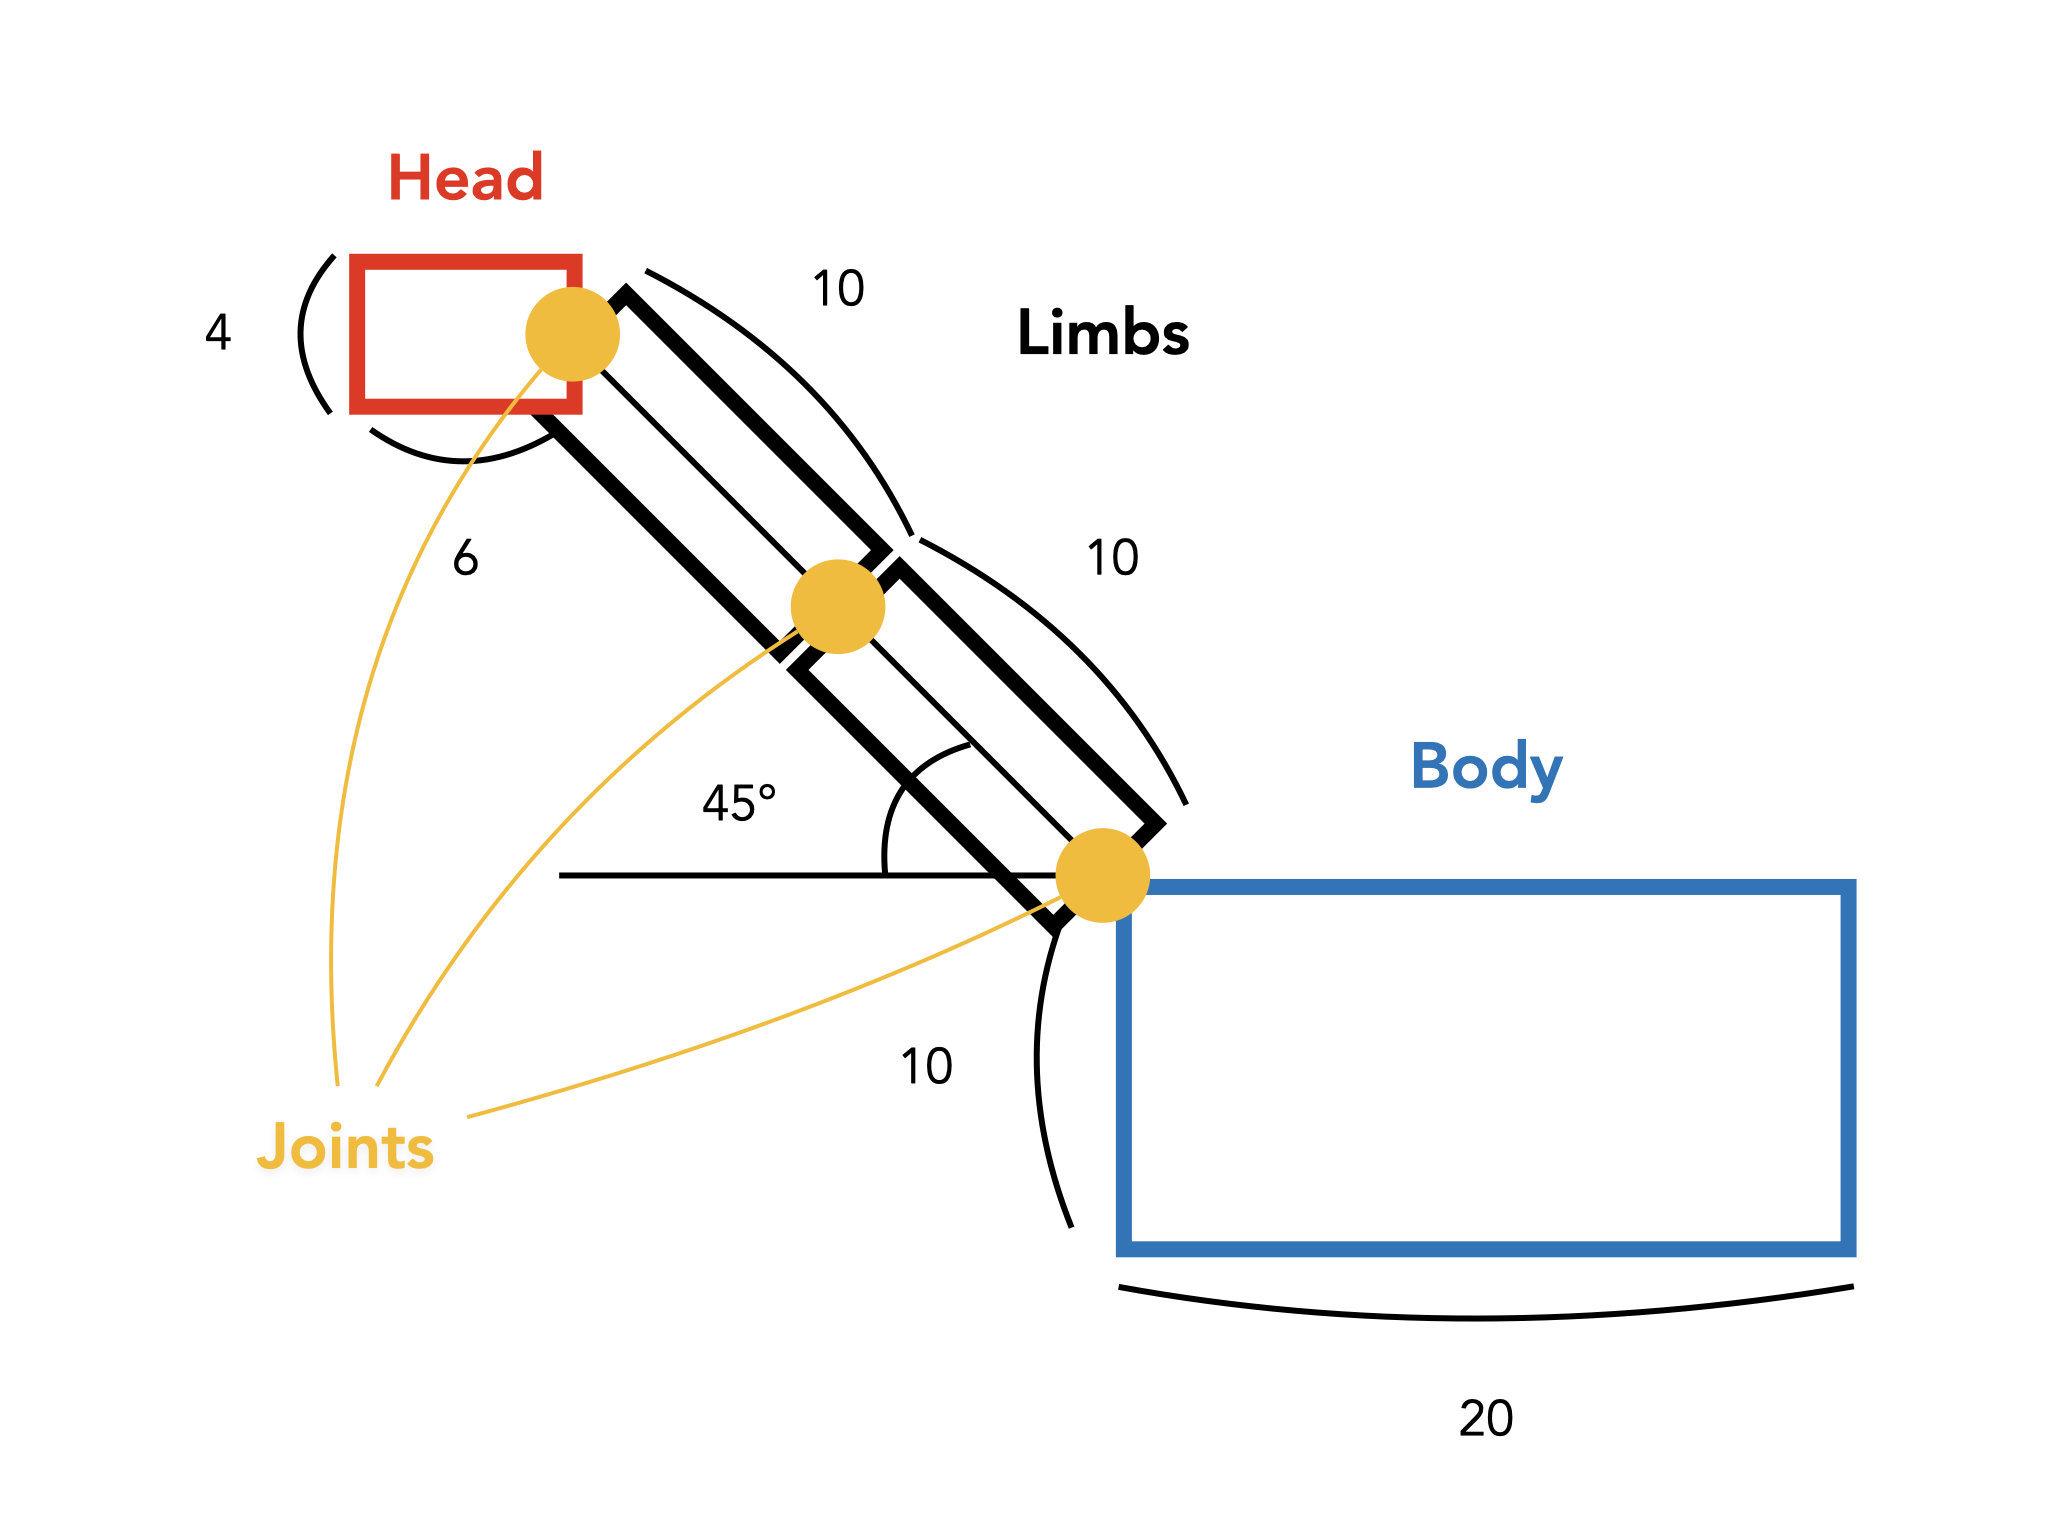
\includegraphics[width=1\textwidth]{figures/pigeon_diagram/pigeon_diagram_001.png}
        \caption{Diagram of the pigeon model}
        \label{fig:pigeon_dimension}
    \end{figure}
  Additionally, the pigeon's head relative to the body is facing the negative direction relative to the x-axis.
  The widths and heights of each limb, head, and body are $(10, 4)$, $(6, 4)$, $(20, 10)$ respectively.
  The initial angles of each limb are oriented at 45 degrees relative to the x-axis, and both the head and the body are oriented parallel to the x axis.
  The body's initial position is at the origin, and is set to move at a constant speed in the negative direction along the x-axis.

\section{Experiment Environments}
% details on all 5 params and reward function differences
  We trained a total of 5 reinforcement learning agents to control the pigeon model: 1 agent for the case where the model is given the baseline task given an unmoving body, 2 agents for cases where the model is given the same task with the body speed of 1, 2 agents for cases where the model is tasked to move its joints to maximize the reward function $r_{fifty\_fifty}$, as defined in Chapter \ref{ch:approach}, under the body speed of 0 and 1 respectively.

  % head target trajectory tracking
    Several additional variables are defined for the pigeon to execute the baseline task as shown in Figure \ref{fig:pigeon_target}.
      \begin{figure}[H]
          \centering
          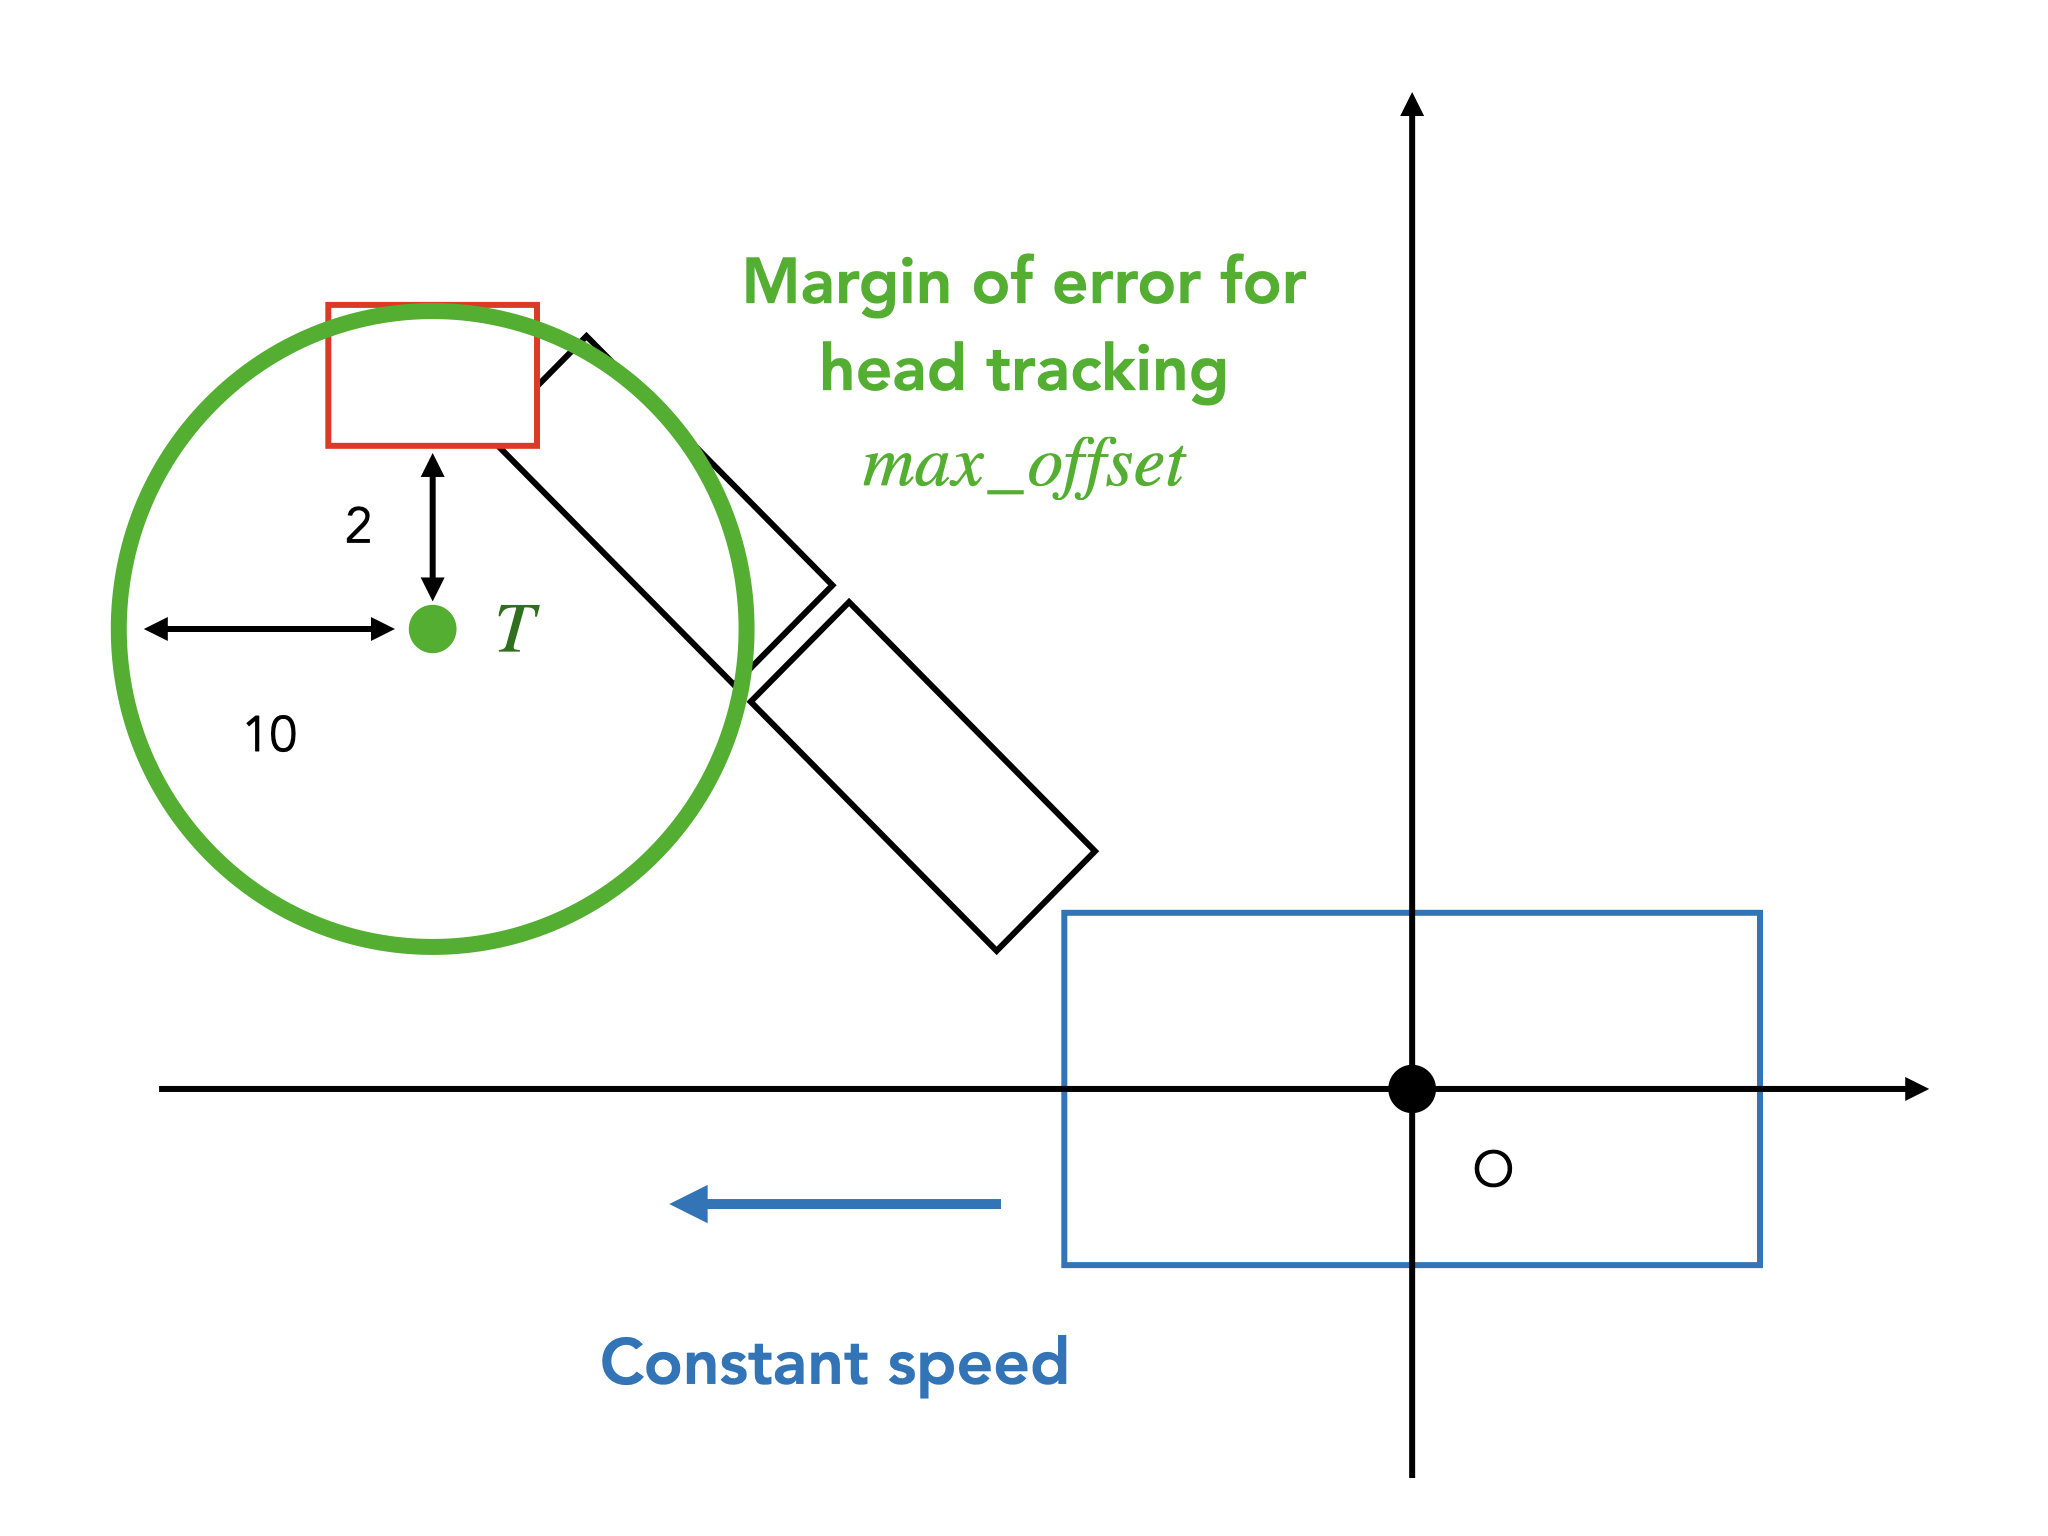
\includegraphics[width=1\textwidth]{figures/pigeon_diagram/pigeon_diagram_002.png}
          \label{fig:pigeon_target}
          \caption{Head trajectory tracking}
      \end{figure}
    $T$ is set at $(0, -2)$ relative to the initial position of the head.
    We set the threshold value for the distance between the target position and the torso's position to 10. As mentioned in Chapter \ref{ch:approach} when the the said distance is below the threshold value, $T$ is reset to be the same position relative to the body as its initial position.
    We set a value $max\_offset$ that represents the margin of error between $T$ and the position of the head.

    % speed = 0
      % _head_stable_manual_reposition_strict_angle
        For the case with an unmoving body, we define a function that generates positive rewards only for timesteps where the distance between the head and $T$ is within $max\_offset = 0.5$. Each reward is bounded within $[0, 1]$ and scaled based on the level of alignment to the x-axis.
          \begin{equation}
              {r_{head\_stable\_manual\_reposition\_strict\_angle}}_t =
              \begin{cases}
                  1 - \frac {\alpha_t} \pi & \text{if $\alpha_t < \frac \pi 6$} \\
                  0 & \text{otherwise}
              \end{cases}
          \end{equation}
        where $\alpha_t$ is the angle of the head at timestep $t$.

    % speed = 1
      % _head_stable_manual_reposition
        For the speed of 1, unlike the case with the unmoving body, $max\_offset = 1$.
        Additionally, alongside $r_{head\_stable\_manual\_reposition\_strict\_angle}$, we define a looser reward function that generates positive rewards as long as the head is within the set margin of error around the target location.
        It is expected that this function would serve as an alternate less strict to the former reward function that produce similar behaviors.
        \begin{equation}
          \begin{aligned}
            {r_{head\_stable\_manual\_reposition}}_t = {r_{head\_stable\_manual\_reposition\_strict\_angle}}_t + \\
              \begin{cases}
                  1 - \frac {\delta_t} {max\_offset} & \text{$\delta_t < max\_offset$} \\
                  0 & \text{otherwise}
              \end{cases}
          \end{aligned}
        \end{equation}
        where $\delta_t$ is the distance between the head and $T$ at timestep $t$.

  % _fifty_fifty
    Preliminary hypotheses regarding retinal stabilization and motion parallax are depicted as the reward function $r_{fifty\_fifty}$. The reward function is used to train agents that represent behaviors derived from such hypotheses under the conditions of both speeds 0 and 1. For both cases, $max\_offset = 1$.
    % external objects
      3 points and their positions are defined to represent 1 static and 2 dynamic objects placed on the surrounding environment of the pigeon.
      The static object's position is $(-30.0, 30.0)$, and the 2 dynamic objects' positions are $(-30.0, 60.0)$, $(-60.0, 30.0)$. The former dynamic object moves at speed 1 in the positive direction along the x-axis, while the latter moves at the same speed in the negative direction along the x-axis.

We constructed OpenAI Gym \cite{brockman2016openai} environments \lstinline|PigeonEnv3Joints| and \lstinline|PigeonRetinalEnv| for conducting reinforcement learning based on the baseline and preliminary hypotheses, respectively.
  Details regarding the environments' code are in Appendix \ref{append:1}.

\section{Reinforcement Learning}
We used SAC to conduct batch training on each deep neural network agent for 3000 epochs. Each deep neural network has one hidden layer containing 256 neurons. Details regarding more rigorous hyperparameter settings are in Appendix \ref{append:2}.

% why we didn't use PPO
  PPO, despite being used often as baseline for many reinforcement learning experiments as we have stated beforehand, was not used for training any of the 5 aforementioned controllers.
  When we attempted to train deep neural network controllers for pigeon models with static bodies using PPO and SAC with $r_{head\_stable\_manual\_reposition}$, we found that the agent trained on SAC had a more stable learning curve and a faster convergence rate than the agent trained on PPO.
  Therefore, we determined that it would be more reliable to use SAC to obtain the desired results.

  \chapter{Results}

% pre-figure explanation
  We rendered the resulting behaviors produced by controllers trained on aforementioned reward functions and environments into images or frames.
  Combining the frames generated for each of the 1000 timesteps and setting as 60 frames per second resulted in 33.35 second videos.
  The time-lapses presented in Figures \ref{fig:manual_trajectory_body_speed_0}, \ref{fig:manual_trajectory_strict_body_speed_1}, \ref{fig:manual_trajectory_not_strict_body_speed_1}, \ref{fig:fifty_fifty_body_speed_0}, and \ref{fig:fifty_fifty_body_speed_1} were created by sampling every $300$ frames within the last 30 seconds of the video.
  The frames' sequential order is from the top left to the bottom right.
  The camera is locked to follow the pigeon's body.
  % 60/5 * [10] = 300


  \begin{figure}[H]
      \centering
      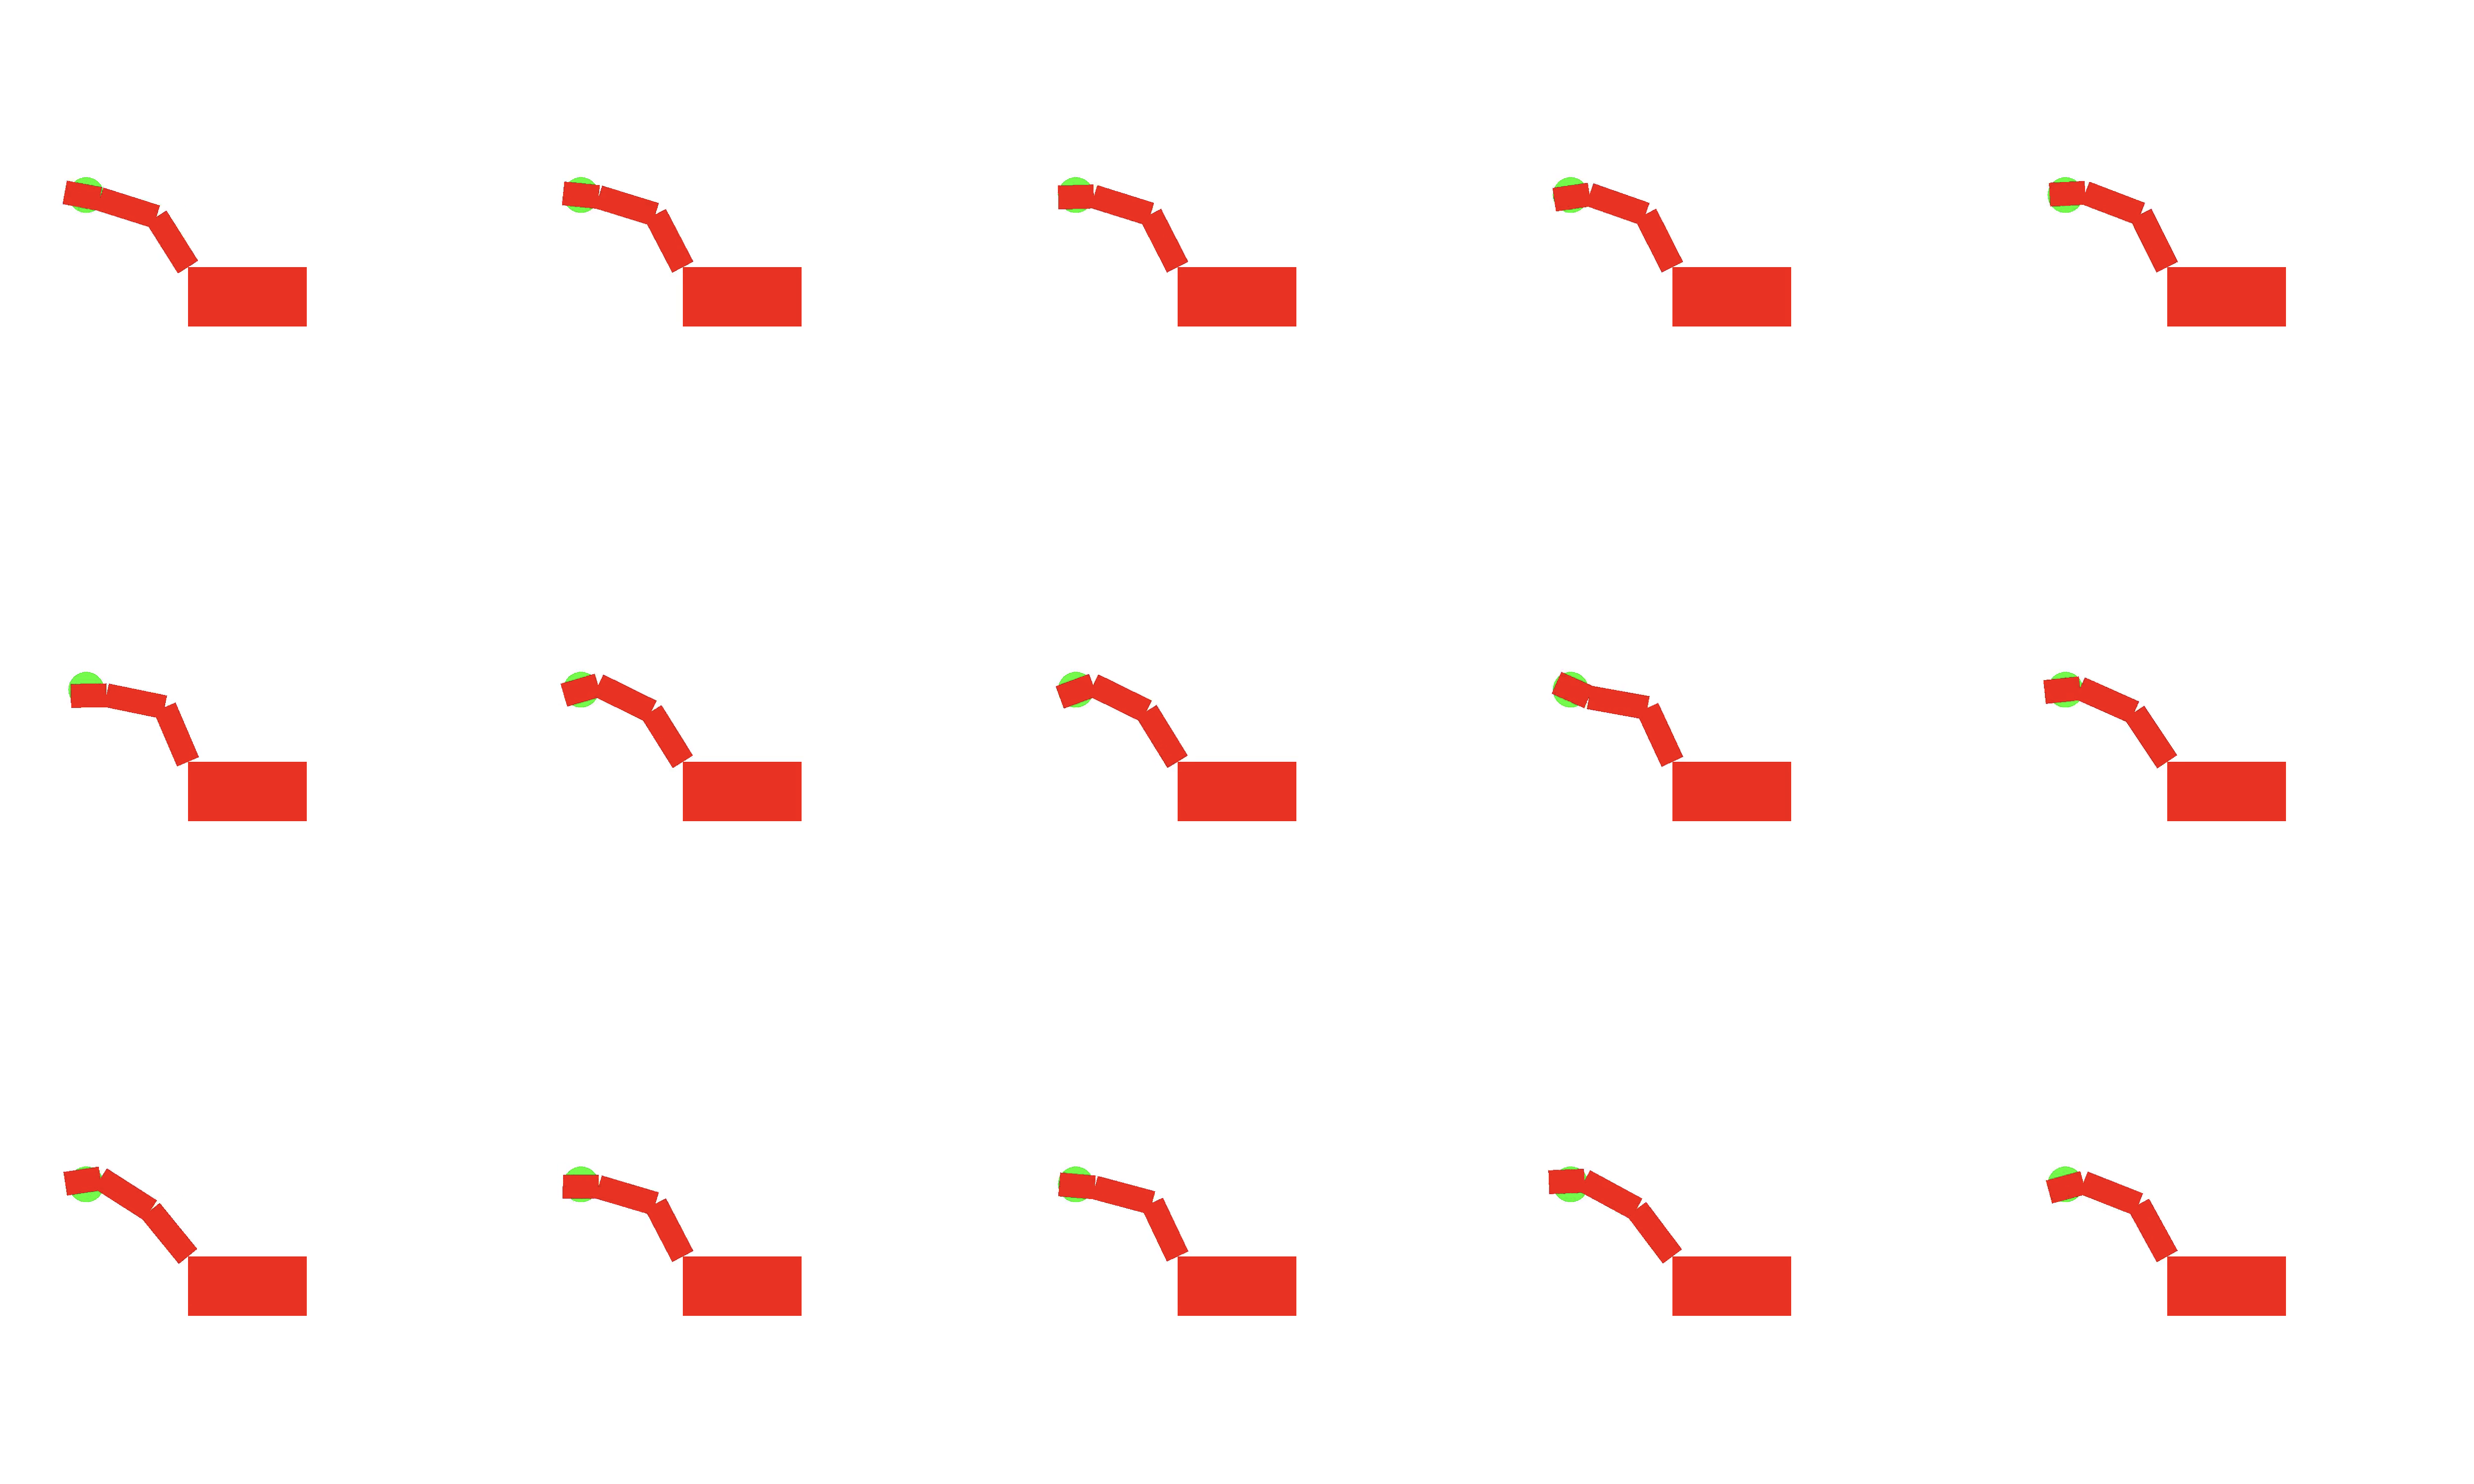
\includegraphics[width=1\textwidth]{figures/frames/frames_001.png}
      \caption{Control of a pigeon model with a static body trained on $r_{head\_stable\_manual\_reposition\_strict\_angle}$ with $max\_offset = 0.5$. The green circle indicate the margin of error around the target head location defined by $max\_offset$.}
      \label{fig:manual_trajectory_body_speed_0}
  \end{figure}

  \begin{figure}[H]
      \centering
      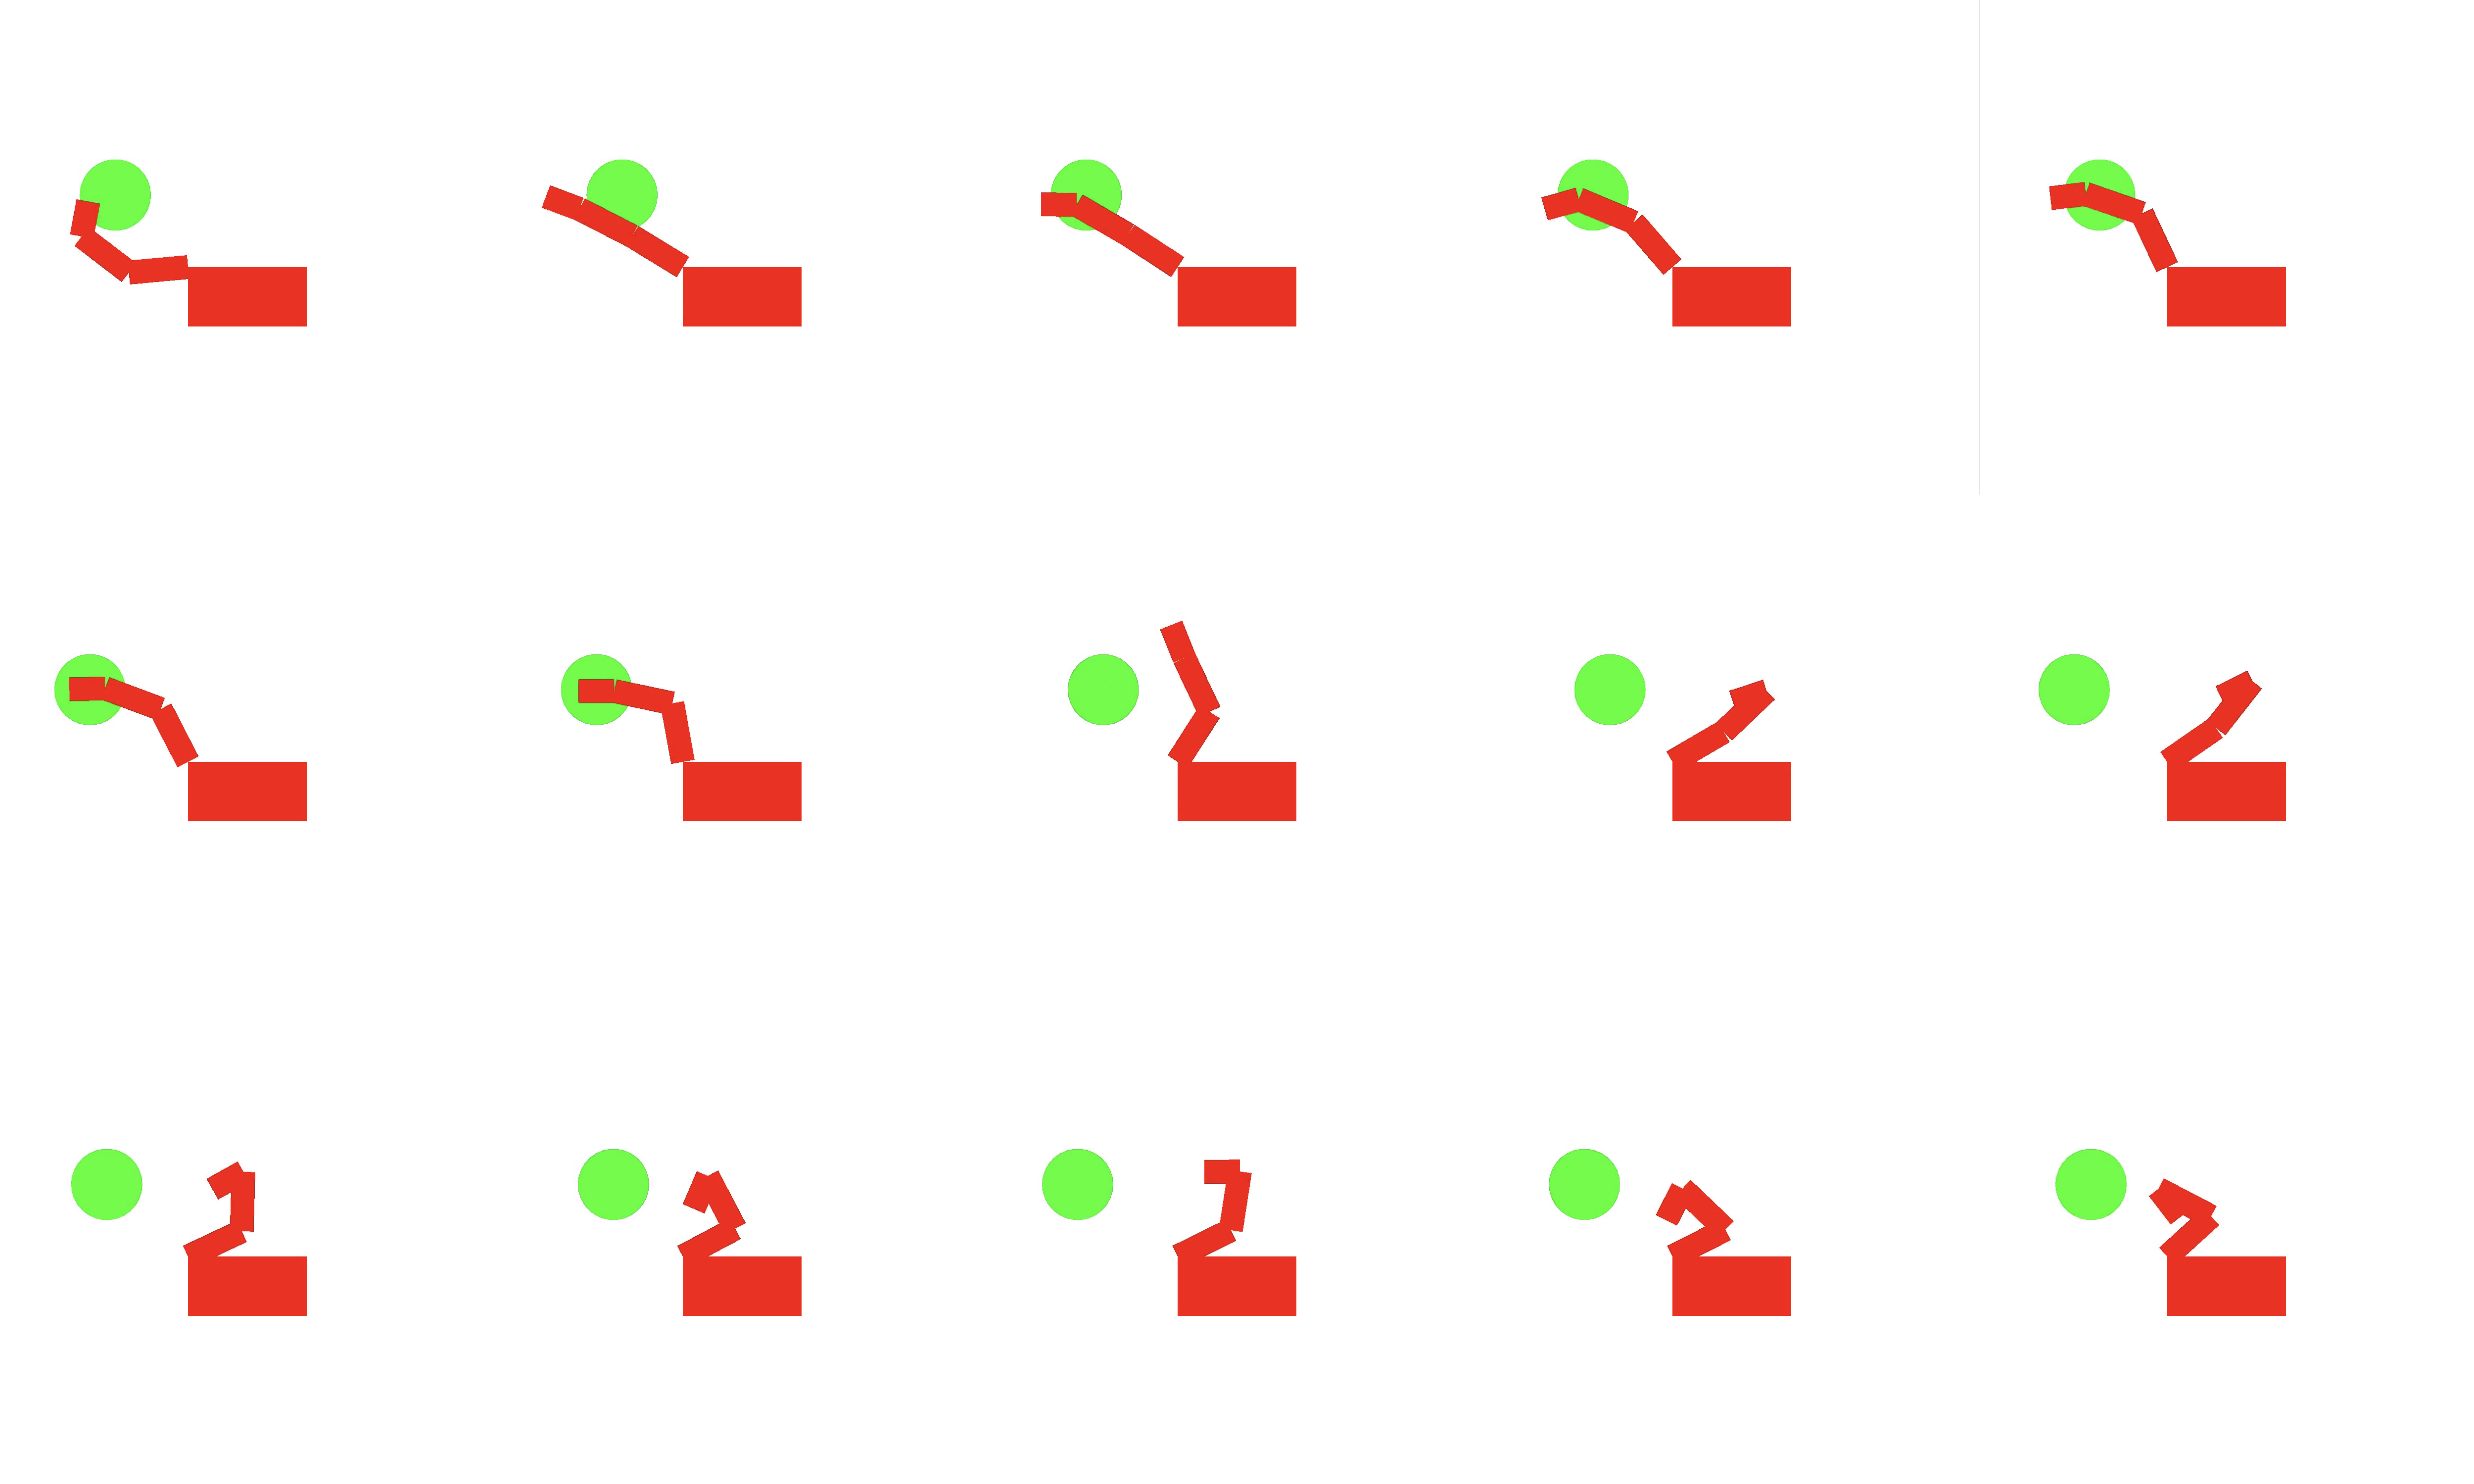
\includegraphics[width=1\textwidth]{figures/frames/frames_002.png}
      \caption{Control of a pigeon model with the body speed of 1 trained on $r_{head\_stable\_manual\_reposition\_strict\_angle}$ with $max\_offset = 1.0$. The green circle indicate the margin of error around the target head location defined by $max\_offset$.}
      \label{fig:manual_trajectory_strict_body_speed_1}
  \end{figure}

  \begin{figure}[H]
      \centering
      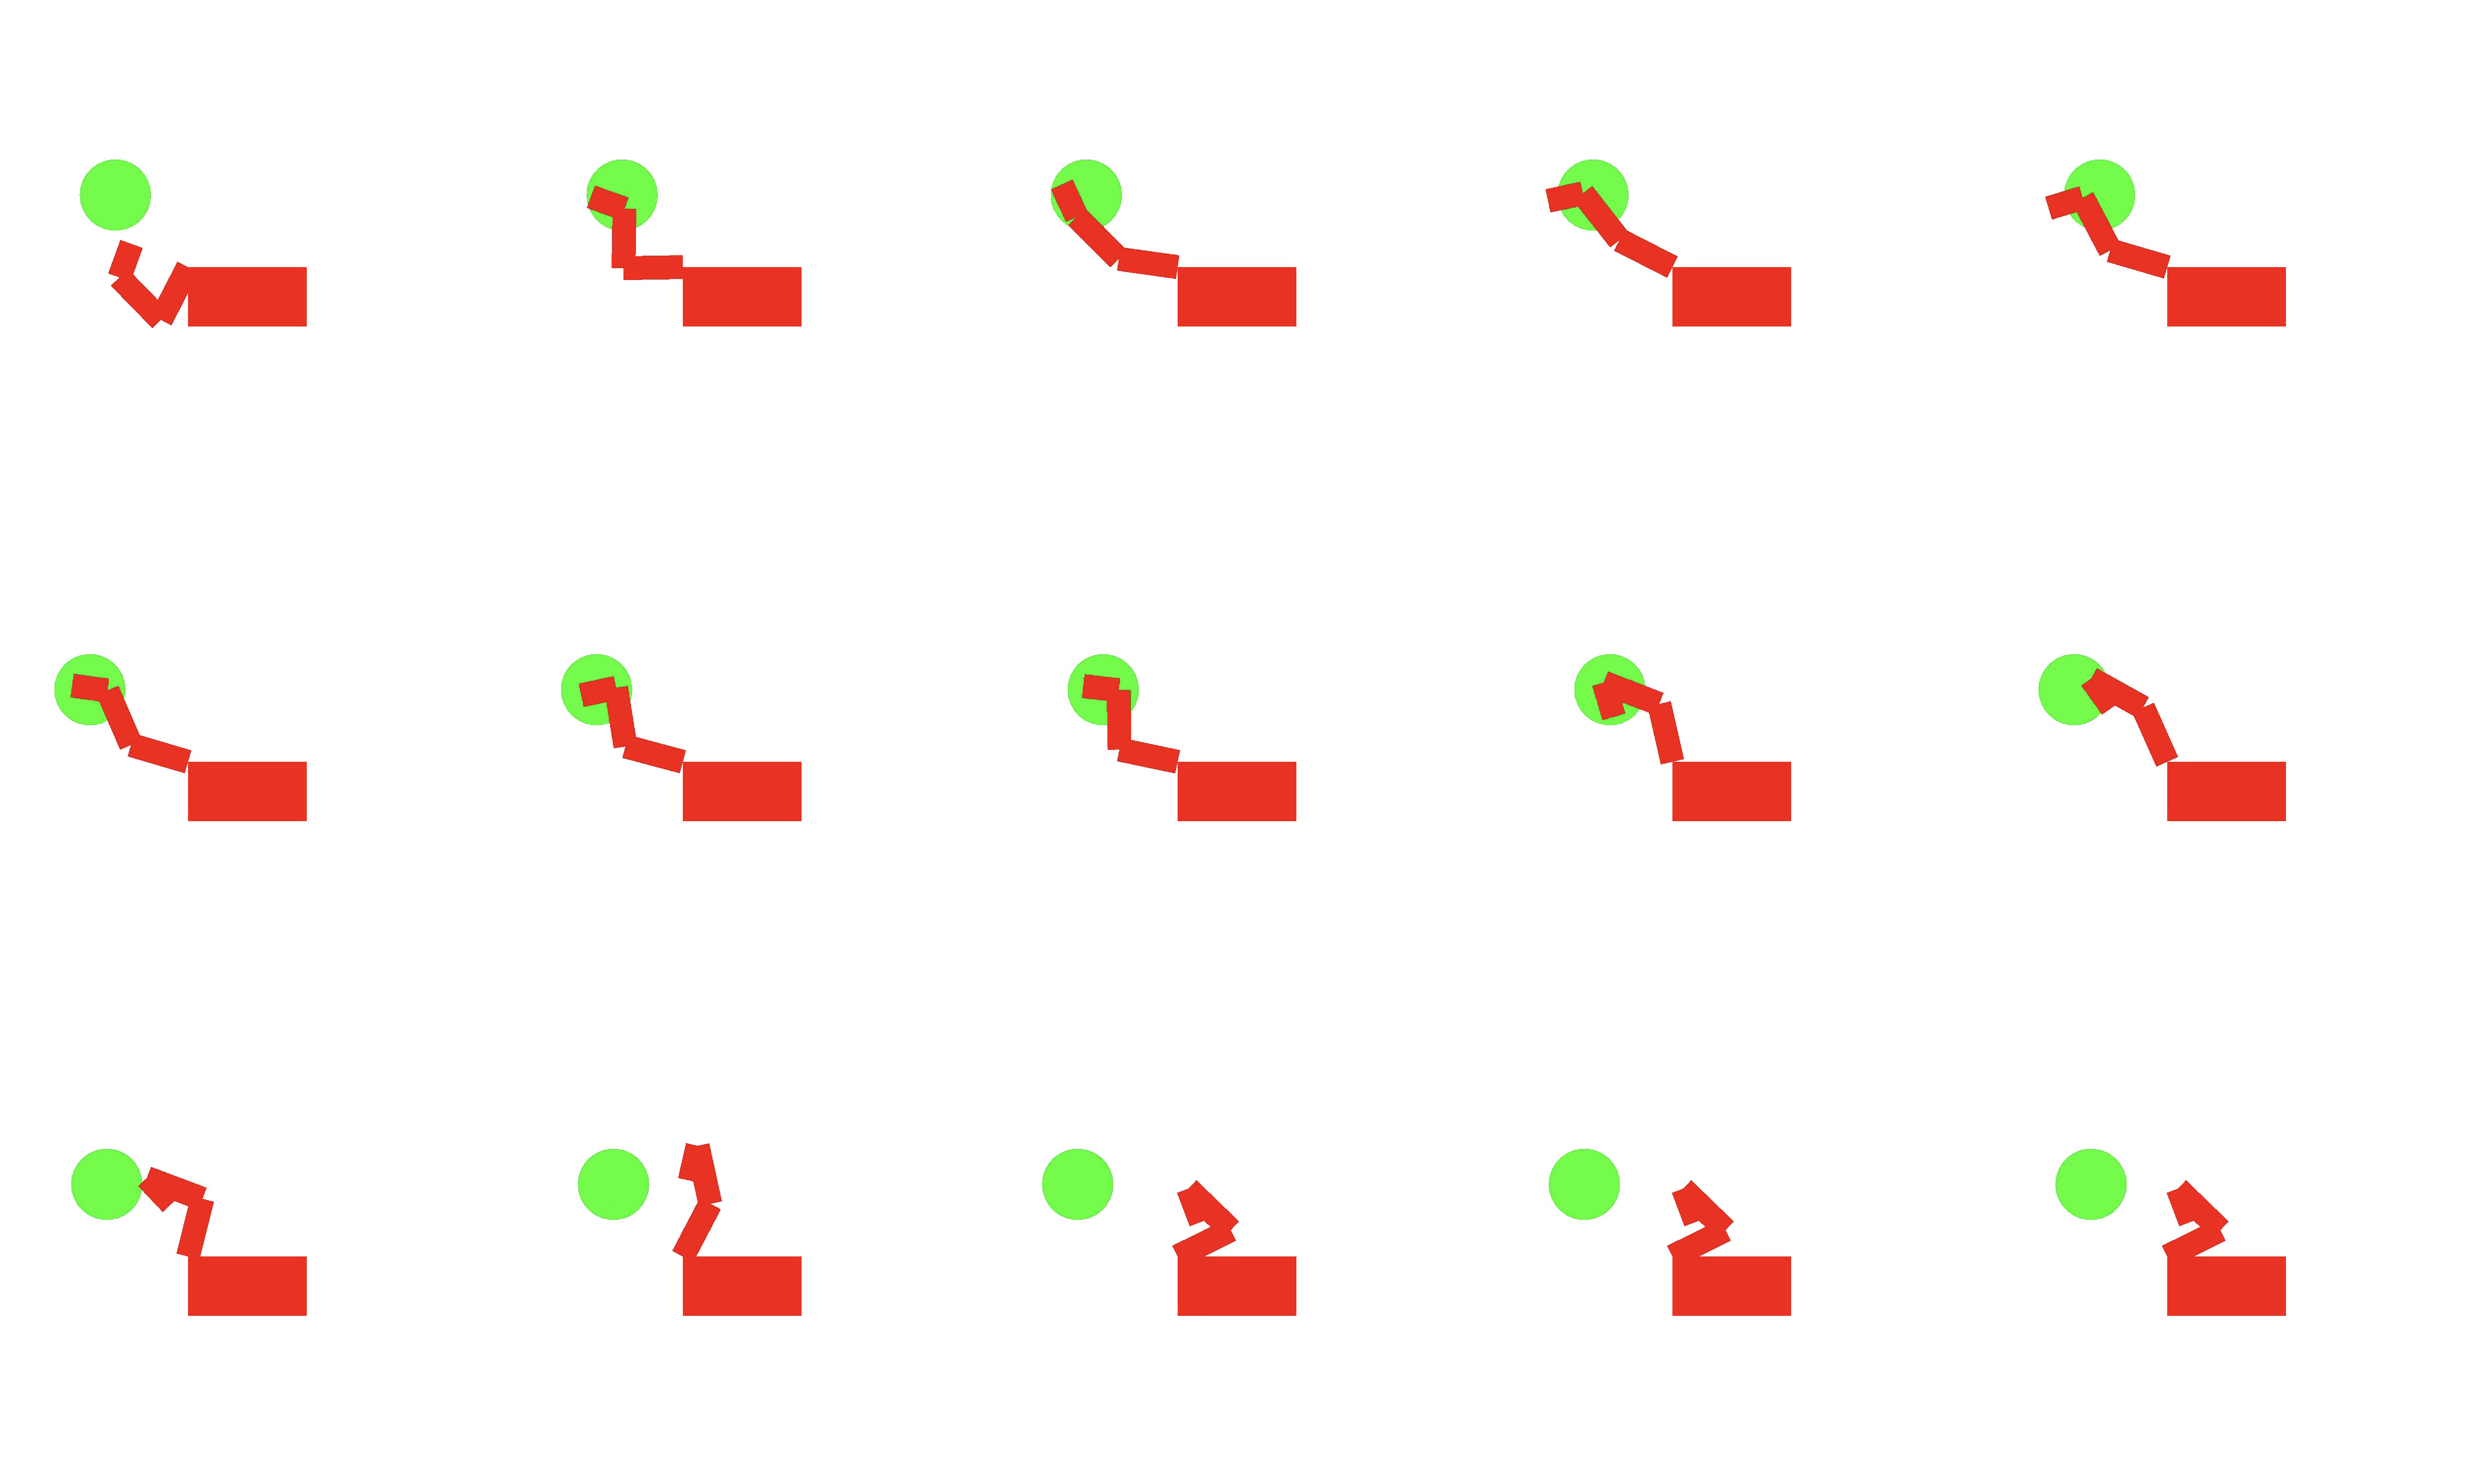
\includegraphics[width=1\textwidth]{figures/frames/frames_003.png}
      \caption{Control of a pigeon model with the body speed of 1 trained on $r_{head\_stable\_manual\_reposition}$ with $max\_offset = 1.0$. The green circle indicate the margin of error around the target head location defined by $max\_offset$.}
      \label{fig:manual_trajectory_not_strict_body_speed_1}
  \end{figure}

  \begin{figure}[H]
      \centering
      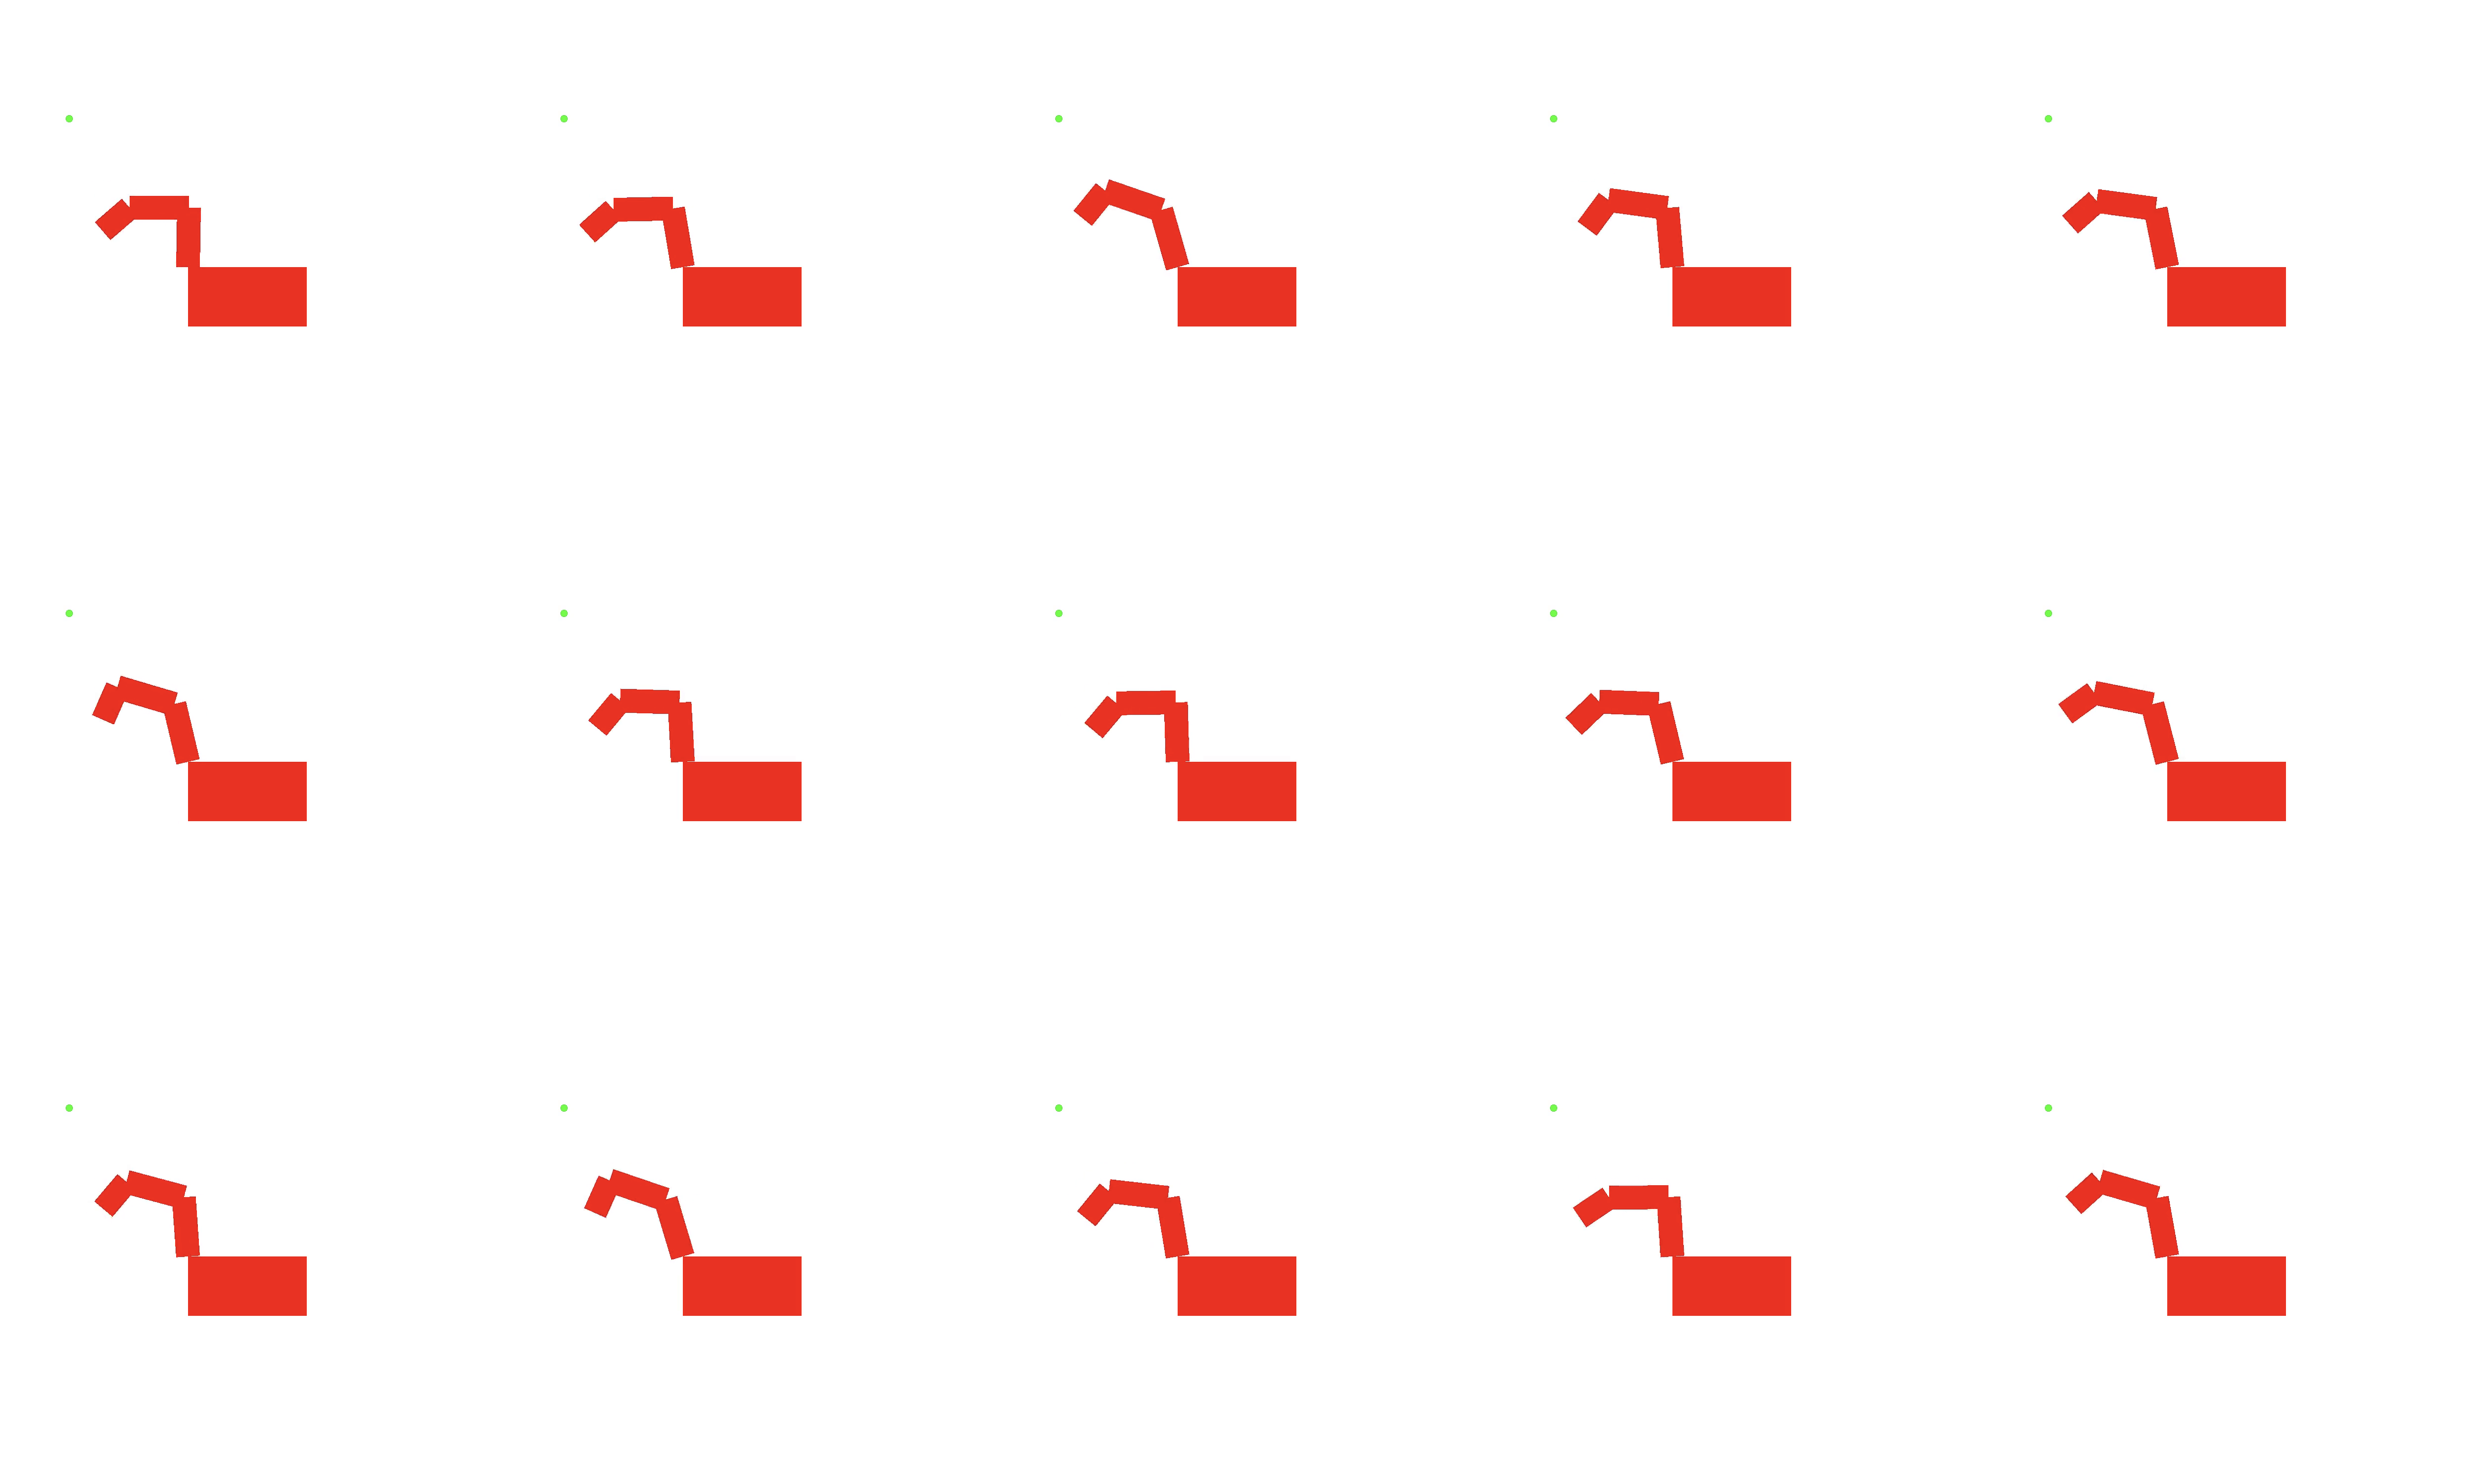
\includegraphics[width=1\textwidth]{figures/frames/frames_004.png}
      \caption{Control of a pigeon model with a static body trained on $r_{fifty\_fifty}$}
      \label{fig:fifty_fifty_body_speed_0}
  \end{figure}

  \begin{figure}[H]
      \centering
      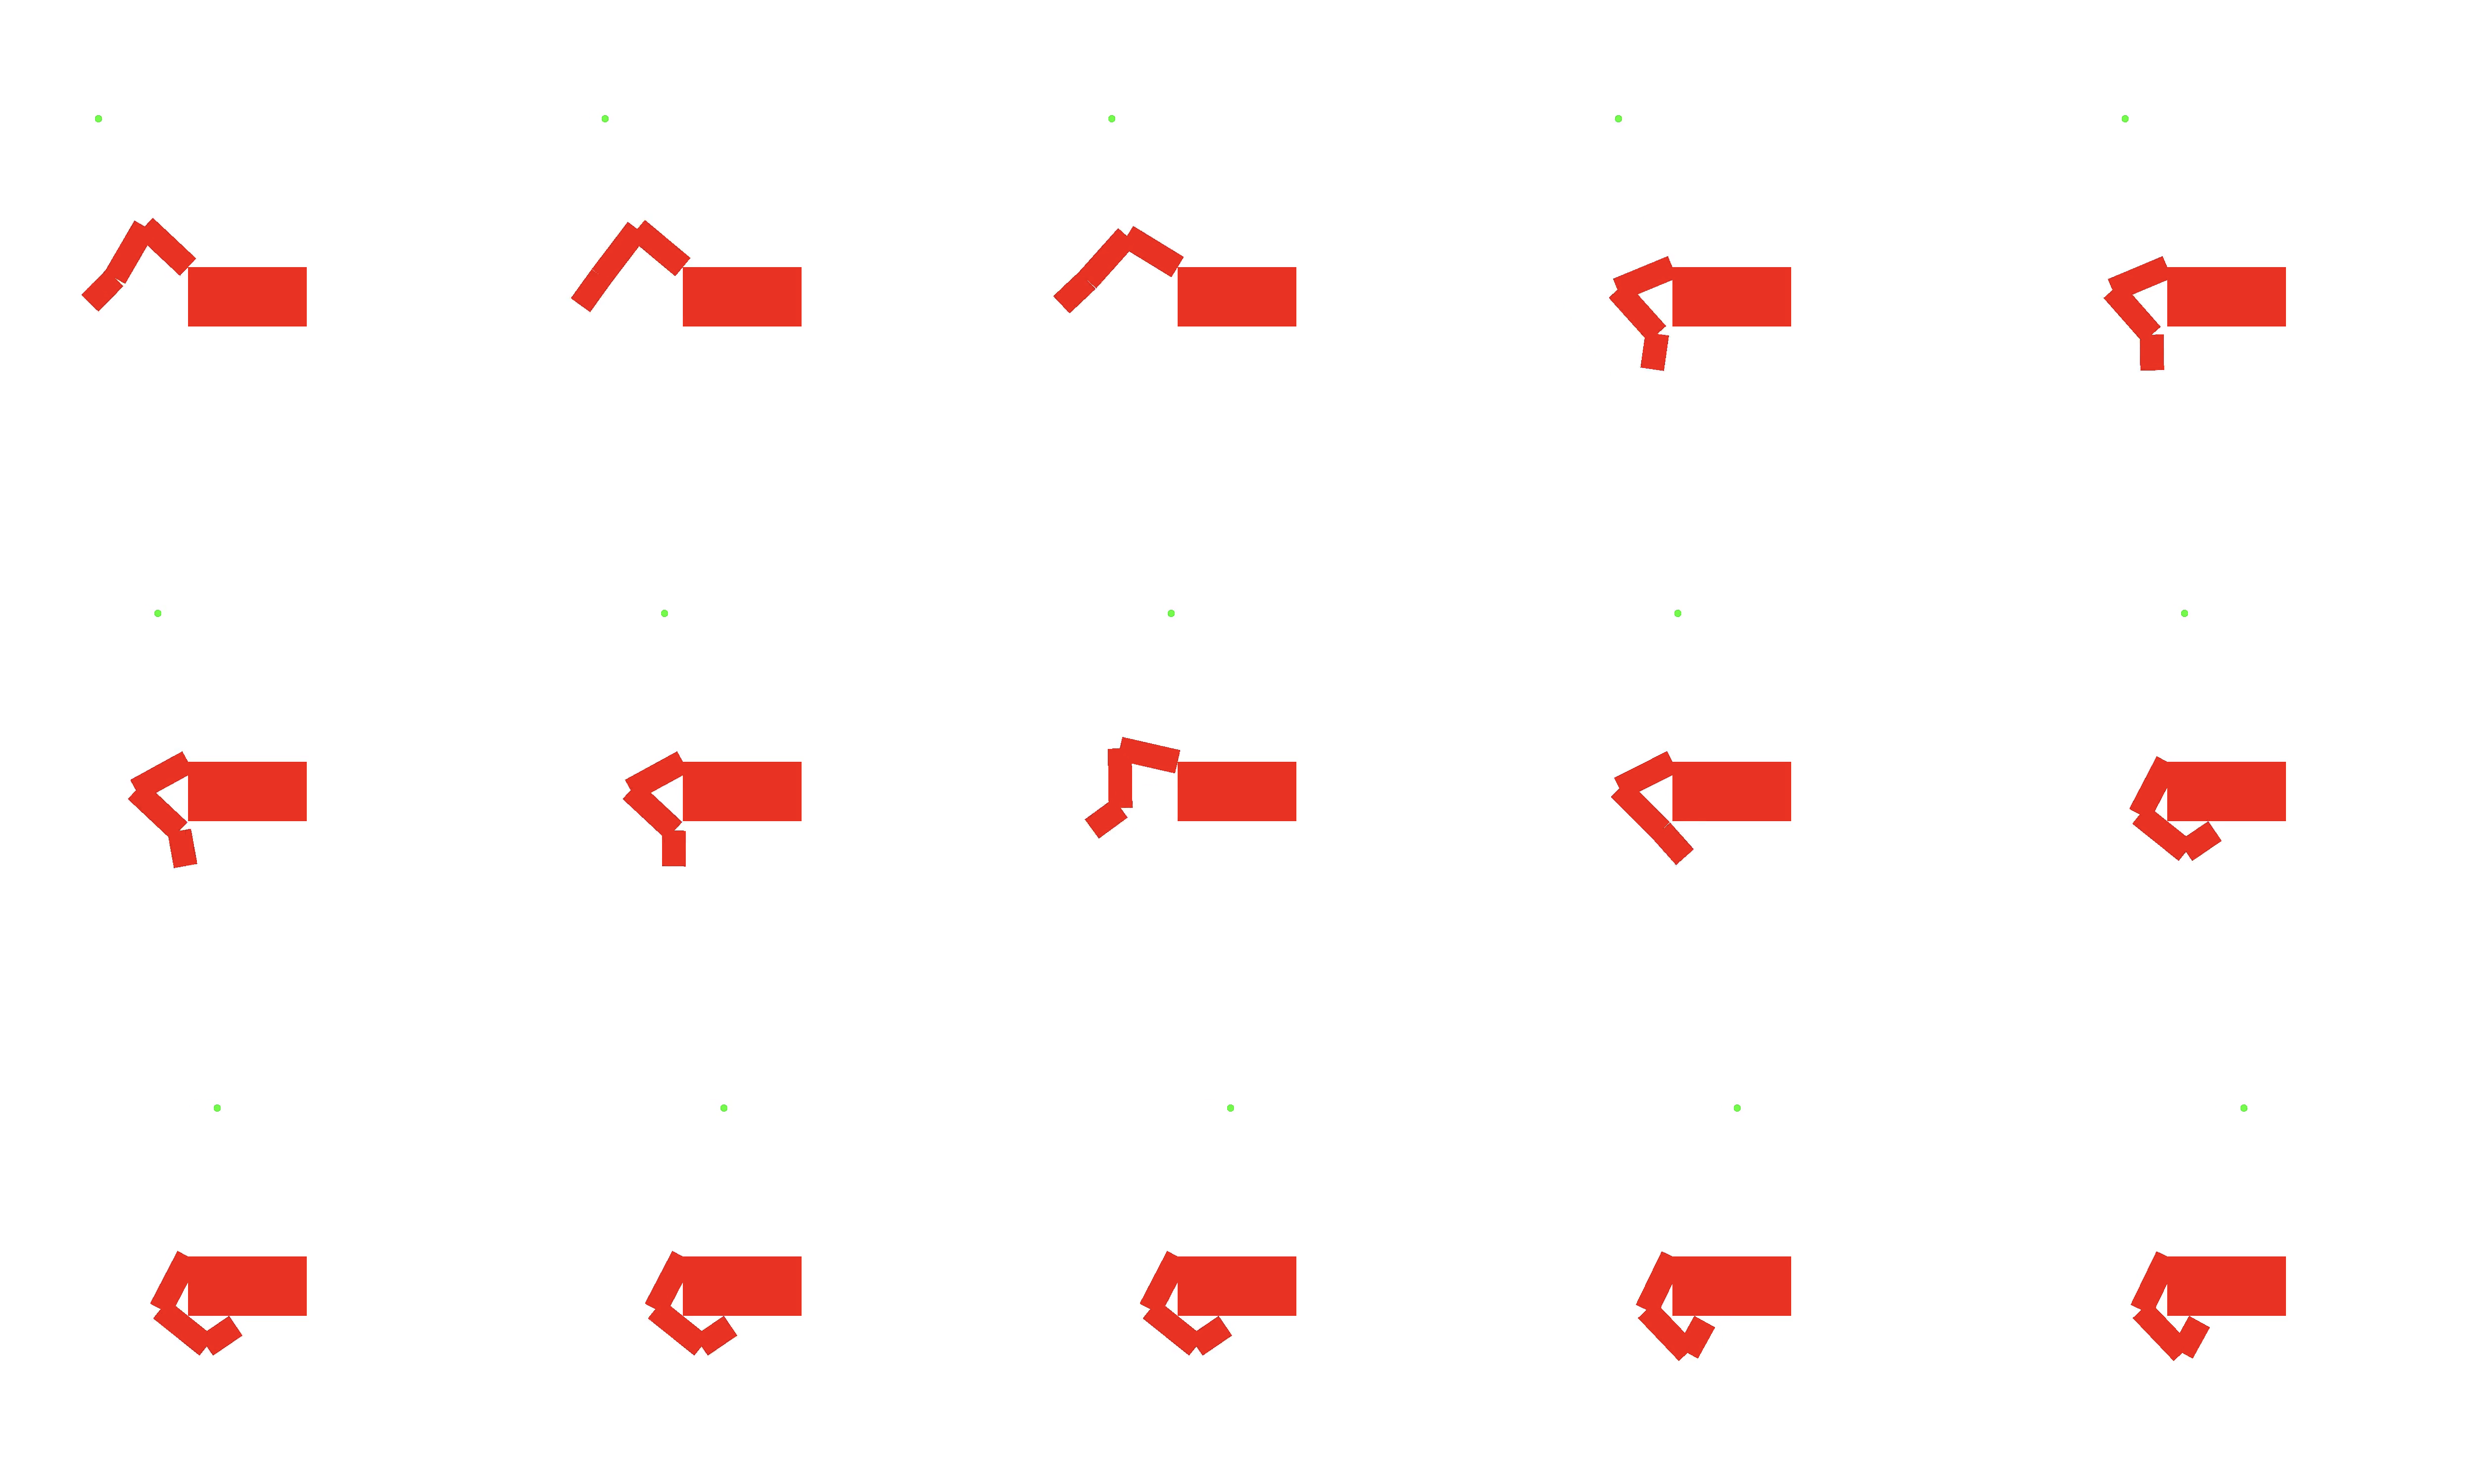
\includegraphics[width=1\textwidth]{figures/frames/frames_005.png}
      \caption{Control of a pigeon model with the body speed of 1 trained on $r_{fifty\_fifty}$}
      \label{fig:fifty_fifty_body_speed_1}
  \end{figure}


% summary of the results
  % 1.
  % 2.

  % 3. head wiggles relatively in the same position

  %\chapter{Analysis}
% variance between the two trajectories/paths

  \chapter{Discussion}
% "results indicate that..."
  % Examining the trajectory of each of the pigeon models' heads,
  % the resulting behavior exhibited by the pigeon model with a fixed body, whose deep reinforcement learning controller was trained on $r_{fifty\_fifty}$, indicate that the combination of visual stabilization and motion parallax are sufficient to generate a behavior that fixes the position of the head, resembling the hold phase in pigeons.

  % On the other hand, the resulting behavior exhibited by the pigeon model with body speed 1, whose deep reinforcement learning controller was trained on the same reward function, indicate that the 2 functionalities are insufficient to produce head-bobbing behaviors in moving bodies during forward locomotion, as he pigeon model did not need to periodically thrust its head forward to maximize Davies' equation depicting motion parallax between objects.

  % Such results indicate that visual stabilization with retinal cells capable of detecting movement in all directions is enough to maximize the sum of external objects' angular velocities within the retina.
    % Examining Davies' equation \ref{davies_motion_parallax}, it can be hypothesized that
    % reinforcement learning controllers trained on reward function that reflect such function would only reproduce head-bobbing behaviors
    % when all objects within the retina are globally static, since the equation does not account for the objects' velocities.
    % Since the external objects in our experiment had objects moving forwards and backwards, such may have automatically increased the reward function depicting Davies' equation of motion parallax per timestep.


% may need a state machine-like mechanism for replication of head-bob
  % composed of the "hold phase" state and the "thrust phase" state
% hierarchical control system
  % hierarchical reinforcement learning should be used for modeling the control system with this hypothesis
% indicates that a hierarchical control system is embedded in pigeons' neurology.
% pattern generating module or functionality, such as central pattern generators seen in the spinal cortex

% head goes downwards during forward locomotion
% lack of muscular strain penalty?

% needs higher details, such as an addition of muscular physics, and progression in incremental modeling
% muscular simulation and their placements upon the skeletal model may lead to more stabilization (cite Geijtenbeek)

  %\input{futurework.tex}


  % Acknowledgements
  \acknowledgements
  Lorem ipsum dolor sit amet, consectetur adipiscing elit. In efficitur porta augue, at interdum nunc lobortis at. Morbi feugiat facilisis justo, vitae maximus dolor. Cras convallis at elit in porta. Fusce lobortis tortor nibh, quis imperdiet arcu luctus quis. Mauris imperdiet urna eu mauris aliquet, vitae tincidunt orci dapibus. Vestibulum convallis elit ut velit accumsan cursus. Pellentesque lacus lacus, blandit eu felis vitae, pellentesque dignissim est.



  % Reference
  \newpage
  %\reference
  \nocite{*}
  %\nocite{*} %Use if you want to list everything listed in bibtex, if not comment it out

  %Bibliography
  %\bibliographystyle{abbrv}

  %ACM SIGCHI Style
  \bibliographystyle{acm-sigchi}
  \bibliography{ref}

  % Appendix
  \appendix
  \section{OpenAI Gym for Simplified Model of Pigeons' Head Control}
% written in Python

% reference to OpenAI Gym library site or paper

\subsection{Usage}
\begin{lstlisting}
PigeonEnv3Joints(self, body_speed = 0,
                 reward_code = "head_stable_manual_reposition",
                 max_offset = 0.5)
\end{lstlisting}
\begin{itemize}
    \item \lstinline|body_speed| indicates the speed in which the pigeon model's body moves.

    \item Each of the following \lstinline|reward_code| are assigned to their respective reward functions.
        \begin{itemize}
          \item \lstinline|"head_stable_manual_reposition"|
              \begin{description}
                  \item Implementation of $r_{head\_stable\_manual\_reposition}$
              \end{description}
          \item \lstinline|"head_stable_manual_reposition_strict_angle"|
              \begin{description}
                  \item Implementation of $r_{head\_stable\_manual\_reposition\_strict\_angle}$
              \end{description}
        \end{itemize}
    \item \lstinline|max_offset| indicates the $max\_offset$ for each reward function to reference.
\end{itemize}

\begin{lstlisting}
PigeonRetinalEnv(self,
                 body_speed = 0,
                 reward_code = "motion_parallax")
\end{lstlisting}

Parallel to \lstinline|PigeonEnv3Joints|, each of the following \lstinline|reward_code| are assigned to their respective reward functions.
\begin{itemize}
  \item \lstinline|"retinal_stabilization"|
      \begin{description}
          \item Implementation of $r_{head\_stabilize}$
          \item Depicts the preliminary hypothesis regarding the functionality of retinal stabilization during the hold phase.
      \end{description}
  \item \lstinline|"motion_parallax"|
      \begin{description}
          \item Implementation of $r_{motion\_parallax}$
          \item Depicts the preliminary hypothesis regarding the functionality of motion parallax induced depth perception during the thrust phase.
      \end{description}
  \item \lstinline|"fifty_fifty"|
      \begin{itemize}
          \item Implementation of $r_{head\_stable\_manual\_reposition\_strict\_angle}$
          \item Sum of rewards produced by  \lstinline|"retinal_stabilization"| and \lstinline|"motion_parallax"|
      \end{itemize}
\end{itemize}

% dependencies
\subsection{Dependencies (Anaconda YAML File)}
The listed versions are recommendations and not strictly necessary for replication
\begin{lstlisting}
name: pigeon-env
channels:
  - conda-forge
  - defaults
dependencies:
  - bzip2=1.0.8=h0d85af4_4
  - ca-certificates=2021.10.8=h033912b_0
  - certifi=2016.9.26=py36_0
  - ffmpeg=4.3.2=h4dad6da_0
  - freetype=2.10.4=h4cff582_1
  - future=0.18.2=py36h79c6626_3
  - gettext=0.19.8.1=h7937167_1005
  - gmp=6.2.1=h2e338ed_0
  - gnutls=3.6.13=h756fd2b_1
  - lame=3.100=h35c211d_1001
  - libcxx=12.0.0=h2f01273_0
  - libffi=3.3=hb1e8313_2
  - libiconv=1.16=haf1e3a3_0
  - libpng=1.6.37=h7cec526_2
  - ncurses=6.3=hca72f7f_2
  - nettle=3.6=hedd7734_0
  - openh264=2.1.1=hfd3ada9_0
  - openssl=1.1.1l=h0d85af4_0
  - pip=21.2.2=py36hecd8cb5_0
  - pybox2d=2.3.10=py36hefe7e0e_1
  - pyglet=1.5.16=py36h79c6626_0
  - python=3.6.13=h88f2d9e_0
  - python_abi=3.6=2_cp36m
  - readline=8.1.2=hca72f7f_1
  - setuptools=58.0.4=py36hecd8cb5_0
  - sqlite=3.37.0=h707629a_0
  - tk=8.6.11=h7bc2e8c_0
  - wheel=0.37.1=pyhd3eb1b0_0
  - x264=1!161.3030=h0d85af4_1
  - xz=5.2.5=h1de35cc_0
  - zlib=1.2.11=h4dc903c_4
  - pip:
    - cloudpickle==2.0.0
    - gym==0.21.0
    - importlib-metadata==4.8.3
    - numpy==1.19.5
    - typing-extensions==4.0.1
    - zipp==3.6.0
\end{lstlisting}

  % \chapter{Appendix}
\section{OpenAI Gym for Simplified Model of Pigeons' Head Control}

% reference to OpenAI Gym library site or paper
% reward function names


\subsection{Manually Defined Head Trajectory (Baseline)}
% Python code as of 01-08-22
\begin{lstlisting}
from Box2D import *
import gym
from gym import spaces

from math import sin, pi, sqrt
import numpy as np
from copy import copy, deepcopy

# anatomical variables ("macros")
BODY_WIDTH = 10
BODY_HEIGHT = 5

LIMB_WIDTH = 5
LIMB_HEIGHT = 2

HEAD_WIDTH = 3

ANGLE_FREEDOM = 0.6

# control variables/macros
MAX_JOINT_TORQUE = 200 #70
MAX_JOINT_SPEED = 5 #10
VELOCITY_WEIGHT = 1.0 #0.9
LIMB_DENSITY = 0.1 ** 3
LIMB_FRICTION = 5

VIEWPORT_SCALE = 6.0
FPS = 60

HEAD_OFFSET_X = 10
HEAD_OFFSET_Y = 2

class PigeonEnv3Joints(gym.Env):
    metadata = {"render.modes": ["human", "rgb_array"], "video.frames_per_second": FPS}

    def __init__(self,
                 body_speed = 0,
                 reward_code = "head_stable_manual_reposition",
                 max_offset = 0.5):
        """
        Action and Observation space
        """

        # 3-dim joints' torque ratios
        self.action_space = spaces.Box(
            np.array([-1.0] * 3).astype(np.float32),
            np.array([1.0] * 3).astype(np.float32),
        )
        # 2-dim head location;
        # 1-dim head angle;
        # 3x2-dim joint angle and angular velocity;
        # 1-dim x-axis of the body
        # [NEW] 2-dim target head location
        high = np.array([np.inf] * 12).astype(np.float32) # formally 10
        self.observation_space = spaces.Box(-high, high)

        """
        Box2D Pigeon Model Params and Initialization
        """
        self.world = b2World()                          # remove in Framework
        self.body = None
        self.joints = []
        self.head = None
        self.bodyRef = [] # for destruction
        self.body_speed = body_speed
        self._pigeon_model()

        """
        Box2D Simulation Params
        """
        self.timeStep = 1.0 / FPS
        self.vel_iters, self.pos_iters = 10, 10

        self.viewer = None

        """
        Assigning a Reward Function
        """
        self._assign_reward_func(reward_code, max_offset)

    """
    Define Reward Function and Necessary Parameters
    """
    def _assign_reward_func(self, reward_code, max_offset):
        if "head_stable_manual_reposition" in reward_code:
            self.max_offset = max_offset

            self.relative_repositioned_head_target_location = np.array(self.head.position) - np.array([0, HEAD_OFFSET_Y])
            self.head_target_location = self.relative_repositioned_head_target_location + np.array(self.body.position)
            self.head_target_angle = self.head.angle
            self.reward_function = self._head_stable_manual_reposition

            if "strict_angle" in reward_code:
                self.reward_function = self._head_stable_manual_reposition_strict_angle

        else:
            raise ValueError("Unknown reward_code")

    """
    Box2D Pigeon Model
    """
    def _pigeon_model(self):
        # params
        body_anchor = np.array([float(-BODY_WIDTH), float(BODY_HEIGHT)])
        limb_width_cos = LIMB_WIDTH / sqrt(2)

        self.bodyRef = []
        # body definition
        self.body = self.world.CreateKinematicBody(
            position = (0, 0),
            shapes = b2PolygonShape(box = (BODY_WIDTH, BODY_HEIGHT)), # x2 in direct shapes def
            linearVelocity = (-self.body_speed, 0),
            angularVelocity = 0,
            )
        self.bodyRef.append(self.body)

        # neck as limbs + joints definition
        self.joints = []
        current_center = deepcopy(body_anchor)
        current_anchor = deepcopy(body_anchor)
        offset = np.array([-limb_width_cos, limb_width_cos])
        prev_limb_ref = self.body
        for i in range(2):
            if i == 0:
                current_center += offset

            else:
                current_center += offset * 2
                current_anchor += offset * 2

            tmp_limb = self.world.CreateDynamicBody(
                position = (current_center[0], current_center[1]),
                fixtures = b2FixtureDef(density = LIMB_DENSITY,
                                        friction = LIMB_FRICTION,
                                        restitution = 0.0,
                                        shape = b2PolygonShape(
                                            box = (LIMB_WIDTH, LIMB_HEIGHT)),
                                        ),
                angle = -pi / 4
            )
            self.bodyRef.append(tmp_limb)

            tmp_joint = self.world.CreateRevoluteJoint(
                bodyA = prev_limb_ref,
                bodyB = tmp_limb,
                anchor = current_anchor,
                lowerAngle = -ANGLE_FREEDOM * b2_pi, # -90 degrees
                upperAngle = ANGLE_FREEDOM * b2_pi,  #  90 degrees
                enableLimit = True,
                maxMotorTorque = MAX_JOINT_TORQUE,
                motorSpeed = 0.0,
                enableMotor = True,
            )

            self.joints.append(tmp_joint)
            prev_limb_ref = tmp_limb

        # head def + joints
        current_center += offset
        current_anchor += offset * 2
        self.head = self.world.CreateDynamicBody(
            position = (current_center[0] - HEAD_WIDTH, current_center[1]),
            fixtures = b2FixtureDef(density = LIMB_DENSITY,
                                    friction = LIMB_FRICTION,
                                    restitution = 0.0,
                                    shape = b2PolygonShape(
                                        box = (HEAD_WIDTH, LIMB_HEIGHT)),
                                    ),
        )
        self.bodyRef.append(self.head)

        head_joint = self.world.CreateRevoluteJoint(
            bodyA = prev_limb_ref,
            bodyB = self.head,
            anchor = current_anchor,
            lowerAngle = -ANGLE_FREEDOM * b2_pi, # -90 degrees
            upperAngle = ANGLE_FREEDOM * b2_pi,  #  90 degrees
            enableLimit = True,
            maxMotorTorque = MAX_JOINT_TORQUE,
            motorSpeed = 0.0,
            enableMotor = True,
        )
        self.joints.append(head_joint)

        # head tracking
        self.head_prev_pos = np.array(self.head.position)
        self.head_prev_ang = self.head.angle

    def _destroy(self):
        for body in self.bodyRef:
            # all associated joints are destroyed implicitly
            self.world.DestroyBody(body)

    def _get_obs(self):
        # (self.head{relative}, self.joints -> obs) operation
        obs = np.array(self.head.position) - np.array(self.body.position)
        obs = np.concatenate((obs, self.head.angle), axis = None)
        for i in range(len(self.joints)):
            obs = np.concatenate((obs, self.joints[i].angle), axis = None)
            obs = np.concatenate((obs, self.joints[i].speed), axis = None)
        obs = np.concatenate((obs, self.body.position[0]), axis = None)

        # complement a target position
        obs = np.concatenate((obs, self.head_target_location - np.array(self.body.position)),
                              axis = None)

        obs = np.float32(obs)
        assert self.observation_space.contains(obs)
        return obs

    def reset(self):
        self._destroy()
        self._pigeon_model()
        return self._get_obs()

    def _head_target_reposition_mechanism(self):
        # detect whether the target head position is behind the body edge or not
        if self.head_target_location[0] > self.body.position[0] - float(BODY_WIDTH + HEAD_OFFSET_X):
            self.head_target_location = np.array(self.body.position) + \
                self.relative_repositioned_head_target_location

        head_dif_loc = np.linalg.norm(np.array(self.head.position) - \
                self.head_target_location)
        head_dif_ang = abs(self.head.angle - self.head_target_angle)
        return head_dif_loc, head_dif_ang

    """
    Modular Reward Functions
    """
    def _head_stable_manual_reposition(self):
        # This method is separated from step(), since there are variables used
        # that are only defined in with this strain of reward functions
        head_dif_loc, head_dif_ang = self._head_target_reposition_mechanism()

        reward = 0
        # threshold reward function with static offset
        if head_dif_loc < self.max_offset:
            reward += 1 - head_dif_loc/self.max_offset

            if head_dif_ang < np.pi / 6: # 30 deg
                reward += 1 - head_dif_ang/ np.pi

        return reward

    def _head_stable_manual_reposition_strict_angle(self):
        head_dif_loc, head_dif_ang = self._head_target_reposition_mechanism()

        reward = 0
        # threshold reward function with static offset
        if head_dif_loc < self.max_offset:
            if head_dif_ang < np.pi / 6: # 30 deg
                reward += 1 - head_dif_ang/ np.pi

        return reward

    def step(self, action):
        assert self.action_space.contains(action)
        # self.world.Step(self.timeStep, self.vel_iters, self.pos_iters)
        # Framework handles this differently
        # Referenced bipedal_walker
        # self.world.Step(1.0 / 50, 6 * 30, 2 * 30)
        self.world.Step(1.0 / FPS, self.vel_iters, self.pos_iters)
        obs = self._get_obs()

        # MOTOR CONTROL
        for i in range(len(self.joints)):
            # Copied from bipedal_walker
            self.joints[i].motorSpeed = float(MAX_JOINT_SPEED * (VELOCITY_WEIGHT ** i) * np.sign(action[i]))
            self.joints[i].maxMotorTorque = float(
                MAX_JOINT_TORQUE * np.clip(np.abs(action[i]), 0, 1)
            )

        reward = self.reward_function()

        done = False
        info = {}
        return obs, reward, done, info

    def render(self, mode = "human"):
        from gym.envs.classic_control import rendering
        if self.viewer is None:
            self.viewer = rendering.Viewer(500, 500)

            # Set ORIGIN POINT relative to camera
            self.camera_trans = b2Vec2(-250, -200) \
            + VIEWPORT_SCALE * self.bodyRef[0].position # camera moves with body

            ## Needs head_stable_manual_reposition reward function to execute
            try:
                # init visualize max_offset
                render_target_area = rendering.make_circle( \
                    radius=VIEWPORT_SCALE * self.max_offset,
                    res=30,
                    filled=True)
                target_translate = rendering.Transform(
                    translation = VIEWPORT_SCALE * self.head_target_location - self.camera_trans,
                    rotation = 0.0,
                    scale = VIEWPORT_SCALE * np.ones(2)
                )
                render_target_area.add_attr(self.target_translate)
                render_target_area.set_color(0.0, 1.0, 0.0)
                self.viewer.add_geom(render_target_area)
            except:
                pass

            # init translation and rotation for each limb
            self.render_polygon_list = []
            self.render_polygon_rotate_list = []
            self.render_polygon_translate_list = []
            for body in self.bodyRef:
                polygon = rendering.FilledPolygon(
                    body.fixtures[0].shape.vertices
                )
                rotate = rendering.Transform(
                    translation = (0.0, 0.0),
                    rotation = body.angle,
                )
                translate = rendering.Transform(
                    translation = VIEWPORT_SCALE * body.position - self.camera_trans,
                    rotation = 0.0,
                    scale = VIEWPORT_SCALE * np.ones(2)
                )
                polygon.set_color(1.0, 0.0, 0.0)
                polygon.add_attr(rotate)
                polygon.add_attr(translate)
                self.render_polygon_list.append(polygon)
                self.render_polygon_rotate_list.append(rotate)
                self.render_polygon_translate_list.append(translate)
                self.viewer.add_geom(polygon)

        # Update ORIGIN POINT relative to camera
        self.camera_trans = b2Vec2(-250, -200) \
        + VIEWPORT_SCALE * self.bodyRef[0].position # camera moves with body

        ## Needs head_stable_manual_reposition reward function to execute
        try:
            # update max_offset shape translation
            new_target_translate = VIEWPORT_SCALE * self.head_target_location - self.camera_trans
            self.target_translate.set_translation(new_target_translate[0], new_target_translate[1])
        except:
            pass

        # update body rotation and translation
        for i, body in enumerate(self.bodyRef):
            self.render_polygon_rotate_list[i].set_rotation(body.angle)
            new_body_translate = VIEWPORT_SCALE * body.position - self.camera_trans
            self.render_polygon_translate_list[i].set_translation(new_body_translate[0], new_body_translate[1])

        return self.viewer.render(return_rgb_array = mode == "rgb_array")

    def close(self):
        # self._destroy()
        # self.world = None

        if self.viewer:
            self.viewer.close()
            self.viewer = None
\end{lstlisting}

  \subsection{Pigeons' Head Control Based on Retinal Inputs}
% Python code as of 01-15-22
\begin{lstlisting}
import PigeonEnv3Joints, VIEWPORT_SCALE
import numpy as np
import gym
from gym import spaces

class PigeonRetinalEnv(PigeonEnv3Joints):

    def __init__(self,
                 body_speed = 0,
                 reward_code = "motion_parallax"):

        """
        Object Location Init (2D Tensor)
        """
        self.objects_position = np.array([[-30.0, 30.0],
                                          [-30.0, 60.0],
                                          [-60.0, 30.0],])
        self.objects_velocity = np.array([[0.0, 0.0],
                                          [1.0, 0.0],
                                          [-1.0, 0.0],])

        """
        Init based on superclass
        Reward function is defined here
        """
        super().__init__(body_speed, reward_code)

        """
        Redefining Observation space
        """
        # 2-dim head location;
        # 1-dim head angle;
        # 3x2-dim joint angle and angular velocity;
        # 1-dim x-axis of the body
        high = np.array([np.inf] * 10).astype(np.float32) # formally 10
        self.observation_space = spaces.Box(-high, high)


    """
    Retinal coords (angles); Within [-np.pi, np.pi]
    """
    def _get_retinal(self, object_position):
        # normalized direction of object from head
        object_direction = object_position - np.array(self.head.position)
        object_direction = object_direction / np.linalg.norm(object_direction)

        sign = np.ones(object_direction.shape[0])
        for i in range(sign.size):
            # is the object above or below the head?
            if object_direction[i][1] < 0:
                sign[i] = -1

        # calculate COSINE angle of object relative to head (positive if above, negative if below)
        # cosine_angle is of size [num_objects,]
        cosine_angle = sign * np.arccos( \
            np.dot(object_direction, np.array([-1.0, 0.0])))

        # differnce in angle between the head angle and sine_angle of head
        relative_angle = cosine_angle + self.head.angle

        # relative_angle should be within [-np.pi, np.pi]
        for i in range(relative_angle.shape[0]):
            if relative_angle[i] < -np.pi:
                k = 1
                while relative_angle[i] < (k + 1) * -np.pi:
                    k += 1
                relative_angle[i] = relative_angle[i] + 2 * np.pi * ((k + 1) // 2)

            elif relative_angle[i] > np.pi:
                k = 1
                while relative_angle[i] > (k + 1) * np.pi:
                    k += 1
                relative_angle[i] = relative_angle[i] - 2 * np.pi * ((k + 1) // 2)

        return relative_angle

    def _get_angular_velocity(self, prev_ang, current_ang):
        angle_velocity = current_ang - prev_ang
        angle_speed = np.absolute(angle_velocity)
        for i in range(angle_velocity.size):
            if angle_speed[i] > np.pi:
                angle_velocity[i] = 2 * np.pi - angle_velocity[i]
            elif angle_speed[i] < -np.pi:
                angle_velocity[i] = 2 * np.pi + angle_velocity[i]
            else:
                pass
        return angle_velocity

    """
    Defining Reward Functions
    """
    def _assign_reward_func(self, reward_code, max_offset = None):
        self.prev_angle = self._get_retinal(self.objects_position)
        if "motion_parallax" in reward_code:
            self.reward_function = self._motion_parallax
        elif "retinal_stabilization" in reward_code:
            self.reward_function = self._retinal_stabilization
        elif "fifty_fifty" in reward_code:
            self.reward_function = self._fifty_fifty
        else:
            raise ValueError("Unknown reward_code")

    def _motion_parallax(self):
        current_angle = self._get_retinal(self.objects_position)

        parallax_velocities = \
            self._get_angular_velocity(current_angle, self.prev_angle)

        reward = 0
        # sum of motion parallax magnitudes
        for i in range(parallax_velocities.size):
            for j in range(i, parallax_velocities.size):
                reward += np.abs(parallax_velocities[i] - parallax_velocities[j])
            # reward += parallax_velocities[i]
        return reward

    def _retinal_stabilization(self):
        reward = 0
        current_angle = self._get_retinal(self.objects_position)
        relative_speeds = \
            np.absolute(self._get_angular_velocity(current_angle, self.prev_angle))
        reward -= np.sum(relative_speeds)
        return reward

    def _fifty_fifty(self):
        reward = 0
        reward += self._retinal_stabilization()
        reward += self._motion_parallax()
        return reward

    def _get_obs(self):
        # (self.head{relative}, self.joints -> obs) operation
        obs = np.array(self.head.position) - np.array(self.body.position)
        obs = np.concatenate((obs, self.head.angle), axis = None)
        for i in range(len(self.joints)):
            obs = np.concatenate((obs, self.joints[i].angle), axis = None)
            obs = np.concatenate((obs, self.joints[i].speed), axis = None)
        obs = np.concatenate((obs, self.body.position[0]), axis = None)
        obs = np.float32(obs)
        assert self.observation_space.contains(obs)
        return obs

    def step(self, action):
        self.prev_angle = self._get_retinal(self.objects_position)
        # alter object
        self.objects_position += self.objects_velocity
        return super().step(action)

    def render(self, mode = "human"):
        from gym.envs.classic_control import rendering
        if self.viewer is None:
            self.render_objects_list = None
            self.render_objects_translate_list = None

        super().render(mode)
        # initialize object rendering pointers
        if self.render_objects_list is None:
            self.render_objects_list = []
            self.render_objects_translate_list = []
            for i in range(self.objects_position.shape[0]):
                object_render_instance = rendering.make_circle( \
                    radius=0.6,
                    res=30,
                    filled=True)
                object_render_instance_translate = rendering.Transform(
                    translation = VIEWPORT_SCALE * \
                        (self.objects_position[i] - self.camera_trans),
                    rotation = 0.0,
                    scale = VIEWPORT_SCALE * np.ones(2)
                )
                object_render_instance.add_attr(object_render_instance_translate)
                object_render_instance.set_color(0.0, 1.0, 0.0)
                self.render_objects_list.append(object_render_instance)
                self.render_objects_translate_list.append(object_render_instance_translate)
                self.viewer.add_geom(object_render_instance)

        # update object translation
        new_object_translate = VIEWPORT_SCALE * self.objects_position - self.camera_trans
        for i in range(self.objects_position.shape[0]):
            self.render_objects_translate_list[i].set_translation( \
                new_object_translate[i][0], new_object_translate[i][1])

        return self.viewer.render(return_rgb_array = mode == "rgb_array")
\end{lstlisting}

  \newpage
  \section{Hyperparameters for Soft Actor Critic Training}
\subsection{}
% SAC training workflow
  % \cite{haarnoja2018soft}
  \begin{figure}[H]
      \centering
      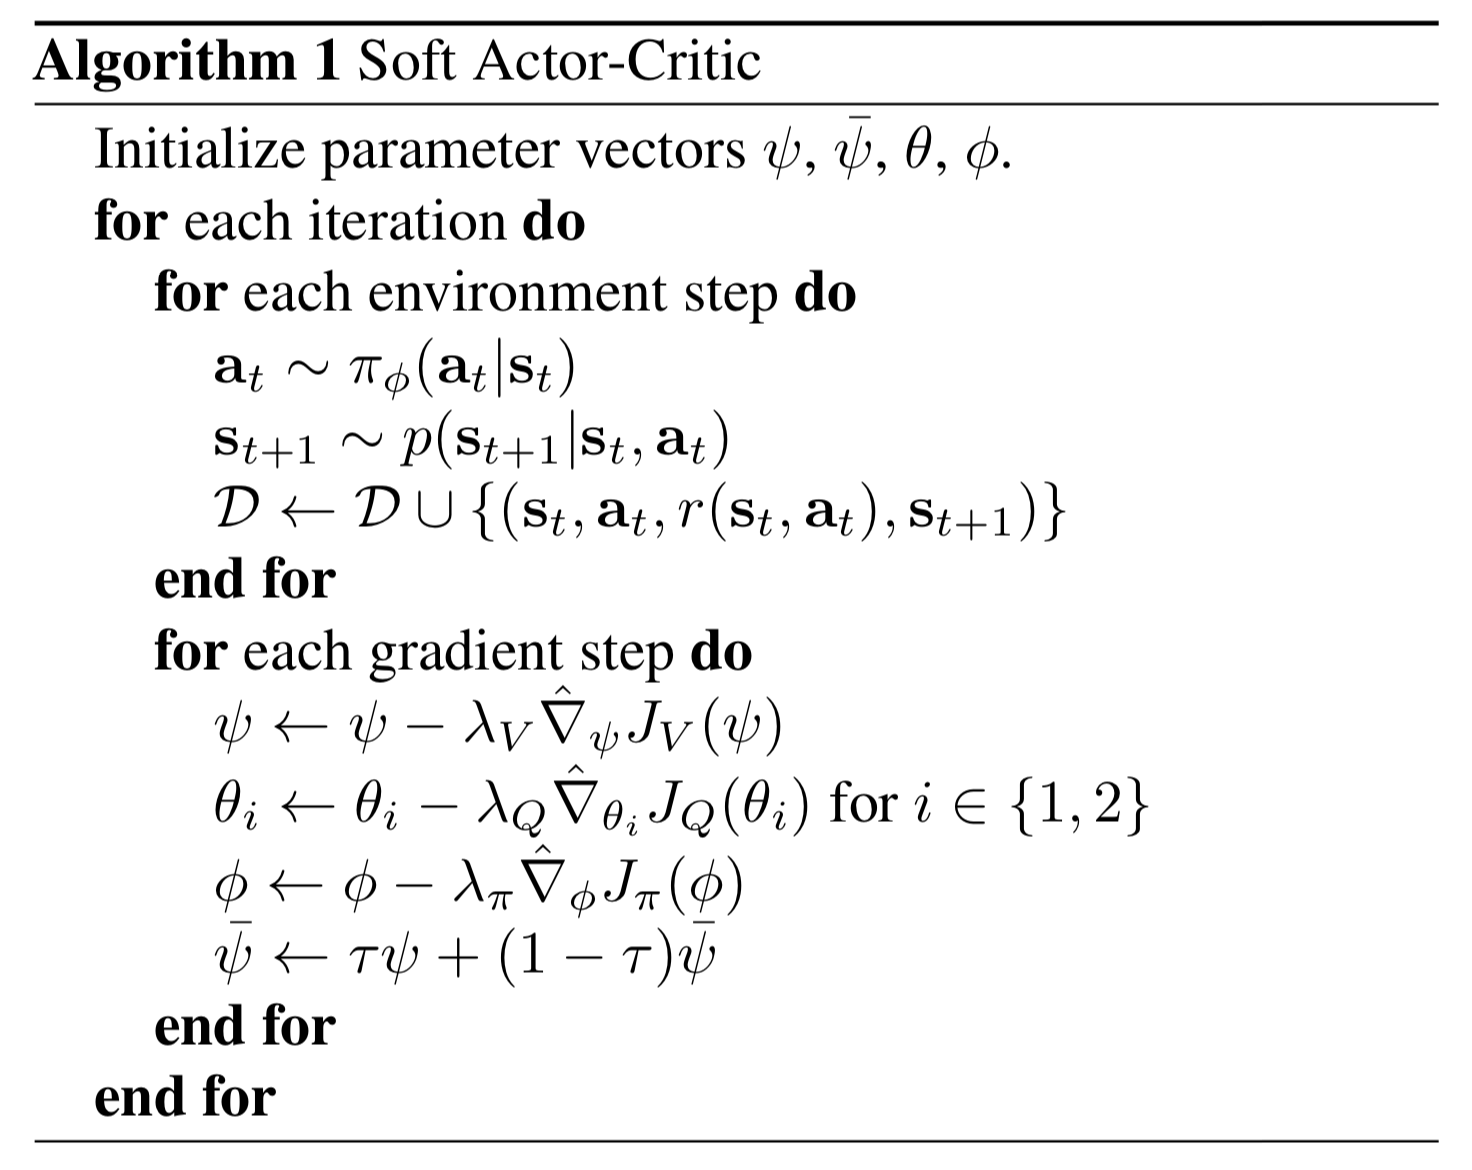
\includegraphics[width=1\textwidth]{figures/external/sac_algorithm.png}
      \caption{Soft Actor Critic algorithm as shown in \cite{haarnoja2018soft}}
      \label{fig:}
  \end{figure}

% batch training
% hidden layer size 256
% epochs 3000

% timesteps per training loop 1000
% param update per training loop 1000
% batch size 256
% replay_buffer_size=int(1E6),

% layer_size=256,
%     replay_buffer_size=int(1E6),
%     algorithm_kwargs=dict(
%         num_epochs=3000,
%         num_eval_steps_per_epoch=5000, % this is for evaluation
%         num_trains_per_train_loop=1000,
%         num_expl_steps_per_train_loop=1000,
%           min_num_steps_before_training=1000,
%           max_path_length=1000,
%         batch_size=256,
%     ),
%     trainer_kwargs=dict(
%         discount=0.99,
%         soft_target_tau=5e-3,
%         target_update_period=1,
%         policy_lr=3E-4,
%         qf_lr=3E-4,
%         reward_scale=1,
%         use_automatic_entropy_tuning=True,
%     ),

  %\newpage
  %\section{Trajectories of the Pigeon Models' Heads and Bodies}

% df_pigeon3joints_bs_0_strict
%\begin{table}
\begin{tabular}{rrrr}
\toprule
 Head Position X &  Head Position Y &  Head Angle &  Body \\
\midrule
      -27.304876 &        19.075607 &   -0.038355 &   0.0 \\
      -27.577311 &        18.579769 &   -0.031786 &   0.0 \\
      -27.494553 &        17.499882 &    0.201975 &   0.0 \\
      -27.249352 &        16.667379 &    0.308322 &   0.0 \\
      -27.186136 &        16.557264 &    0.208435 &   0.0 \\
      -27.192219 &        16.911526 &    0.057138 &   0.0 \\
      -27.189756 &        17.275890 &   -0.097712 &   0.0 \\
      -27.049141 &        16.997484 &   -0.065291 &   0.0 \\
      -26.865608 &        16.439638 &   -0.008119 &   0.0 \\
      -26.797728 &        16.537712 &   -0.139040 &   0.0 \\
      -27.073948 &        17.094383 &   -0.197257 &   0.0 \\
      -27.422674 &        17.489517 &   -0.130617 &   0.0 \\
      -27.518871 &        17.204578 &   -0.052325 &   0.0 \\
      -27.269234 &        16.655300 &   -0.071561 &   0.0 \\
      -27.032854 &        16.694185 &   -0.189525 &   0.0 \\
      -26.886255 &        16.995230 &   -0.209963 &   0.0 \\
      -26.808128 &        16.882746 &   -0.070797 &   0.0 \\
      -26.753113 &        16.495691 &    0.156086 &   0.0 \\
      -27.096411 &        16.695253 &    0.228439 &   0.0 \\
      -27.679838 &        17.276365 &    0.115987 &   0.0 \\
      -27.716311 &        17.286760 &    0.215652 &   0.0 \\
      -27.594442 &        16.990776 &    0.259060 &   0.0 \\
      -27.482189 &        16.884798 &    0.169223 &   0.0 \\
      -27.496002 &        17.422668 &    0.110828 &   0.0 \\
      -27.353428 &        17.916601 &    0.160308 &   0.0 \\
      -27.237112 &        17.775375 &    0.187354 &   0.0 \\
      -27.155123 &        17.515591 &    0.117503 &   0.0 \\
      -27.039532 &        17.252043 &    0.029975 &   0.0 \\
      -26.876362 &        16.883533 &   -0.049080 &   0.0 \\
      -27.015635 &        16.919577 &   -0.057907 &   0.0 \\
      -27.384508 &        17.335890 &   -0.000894 &   0.0 \\
      -27.441128 &        17.549660 &    0.084353 &   0.0 \\
      -27.175114 &        17.190742 &    0.142067 &   0.0 \\
      -26.880850 &        16.889742 &    0.070535 &   0.0 \\
      -26.635960 &        16.757721 &   -0.030030 &   0.0 \\
      -26.857306 &        17.102591 &   -0.068790 &   0.0 \\
      -27.157637 &        17.350435 &    0.015342 &   0.0 \\
      -27.111441 &        17.209986 &    0.146411 &   0.0 \\
      -26.952597 &        16.871920 &    0.186299 &   0.0 \\
      -27.190744 &        17.208944 &    0.024484 &   0.0 \\
      -27.415495 &        17.800333 &   -0.049754 &   0.0 \\
      -27.322577 &        18.049294 &    0.039059 &   0.0 \\
      -27.028593 &        17.653744 &    0.103827 &   0.0 \\
      -26.899956 &        17.269110 &    0.031007 &   0.0 \\
      -26.773186 &        16.842817 &   -0.045810 &   0.0 \\
      -26.970423 &        16.922556 &   -0.185577 &   0.0 \\
      -27.446539 &        17.452503 &   -0.259144 &   0.0 \\
      -27.644125 &        17.661354 &   -0.169263 &   0.0 \\
      -27.376221 &        17.225924 &   -0.102175 &   0.0 \\
      -26.989210 &        16.998186 &   -0.180996 &   0.0 \\
      -26.882605 &        17.078121 &   -0.183264 &   0.0 \\
      -27.024052 &        17.125710 &   -0.068729 &   0.0 \\
      -27.084990 &        16.891626 &    0.070905 &   0.0 \\
      -27.143610 &        17.163639 &    0.157631 &   0.0 \\
      -27.079412 &        17.598684 &    0.221606 &   0.0 \\
      -26.988773 &        17.440205 &    0.243884 &   0.0 \\
      -27.120436 &        17.173876 &    0.150763 &   0.0 \\
      -27.467585 &        17.512598 &    0.089051 &   0.0 \\
      -27.446230 &        17.618921 &    0.178694 &   0.0 \\
      -27.209023 &        17.219507 &    0.239971 &   0.0 \\
      -27.106245 &        17.281261 &    0.128058 &   0.0 \\
      -26.895344 &        17.284111 &    0.020263 &   0.0 \\
      -26.745876 &        17.047892 &   -0.072857 &   0.0 \\
      -26.926460 &        17.028566 &   -0.078692 &   0.0 \\
      -27.137627 &        16.847263 &    0.050939 &   0.0 \\
      -27.329538 &        17.209749 &    0.120326 &   0.0 \\
      -27.252331 &        17.512678 &    0.197504 &   0.0 \\
      -26.944109 &        17.201473 &    0.249432 &   0.0 \\
      -26.823168 &        16.953922 &    0.159788 &   0.0 \\
      -26.785299 &        16.610653 &    0.072182 &   0.0 \\
      -27.158392 &        16.947599 &   -0.095914 &   0.0 \\
      -27.532909 &        17.534559 &   -0.169564 &   0.0 \\
      -27.532759 &        17.571167 &   -0.054097 &   0.0 \\
      -27.162556 &        17.007933 &    0.028870 &   0.0 \\
      -26.968990 &        16.775640 &   -0.063196 &   0.0 \\
      -27.119158 &        17.023539 &   -0.091715 &   0.0 \\
      -27.329718 &        17.247707 &   -0.001904 &   0.0 \\
      -27.175770 &        16.936451 &    0.035376 &   0.0 \\
      -26.826460 &        16.629219 &   -0.037041 &   0.0 \\
      -26.701733 &        16.911808 &   -0.181956 &   0.0 \\
      -26.977730 &        17.467615 &   -0.241783 &   0.0 \\
      -27.218513 &        17.347315 &   -0.116718 &   0.0 \\
      -27.383358 &        16.918684 &   -0.084888 &   0.0 \\
      -27.493486 &        16.832197 &   -0.082509 &   0.0 \\
      -27.618322 &        17.232748 &   -0.008339 &   0.0 \\
      -27.580452 &        17.711700 &    0.049982 &   0.0 \\
      -27.423685 &        17.548685 &    0.080887 &   0.0 \\
      -27.154505 &        17.278011 &    0.016380 &   0.0 \\
      -26.837685 &        17.012056 &   -0.064882 &   0.0 \\
      -26.743990 &        16.871838 &   -0.089968 &   0.0 \\
      -27.088316 &        17.175949 &    0.029844 &   0.0 \\
      -27.380962 &        17.466457 &    0.096239 &   0.0 \\
      -27.488445 &        17.603403 &    0.073795 &   0.0 \\
      -27.461626 &        17.571144 &   -0.070236 &   0.0 \\
      -27.444609 &        17.716442 &   -0.204754 &   0.0 \\
      -27.121601 &        17.288090 &   -0.264451 &   0.0 \\
      -26.801157 &        16.939459 &   -0.214612 &   0.0 \\
      -26.928747 &        17.198898 &   -0.115954 &   0.0 \\
      -27.245375 &        17.636007 &   -0.056315 &   0.0 \\
      -27.341654 &        17.376209 &    0.078965 &   0.0 \\
      -27.062843 &        16.619247 &    0.165419 &   0.0 \\
      -26.934431 &        16.520069 &    0.060055 &   0.0 \\
      -27.028954 &        16.997379 &   -0.109247 &   0.0 \\
      -27.384865 &        17.588833 &   -0.180818 &   0.0 \\
      -27.545084 &        17.410919 &   -0.052076 &   0.0 \\
      -27.284187 &        16.722105 &    0.028364 &   0.0 \\
      -27.089981 &        16.614590 &   -0.075130 &   0.0 \\
      -27.165833 &        17.013269 &   -0.113715 &   0.0 \\
      -27.398373 &        17.469053 &   -0.049731 &   0.0 \\
      -27.466965 &        17.315344 &   -0.042908 &   0.0 \\
      -27.270395 &        17.067860 &   -0.155251 &   0.0 \\
      -27.022774 &        17.266594 &   -0.287845 &   0.0 \\
      -26.754108 &        17.456192 &   -0.293384 &   0.0 \\
      -26.506445 &        17.015203 &   -0.116411 &   0.0 \\
      -26.338758 &        16.414825 &    0.065597 &   0.0 \\
      -26.750753 &        16.622686 &    0.033558 &   0.0 \\
      -27.390520 &        17.426517 &   -0.189296 &   0.0 \\
      -27.562180 &        17.963606 &   -0.454347 &   0.0 \\
      -27.248177 &        17.582987 &   -0.516535 &   0.0 \\
      -26.778385 &        16.865562 &   -0.417420 &   0.0 \\
      -26.364721 &        16.511133 &   -0.504197 &   0.0 \\
      -26.256121 &        16.644579 &   -0.510978 &   0.0 \\
      -26.377121 &        17.082438 &   -0.414939 &   0.0 \\
      -26.308004 &        17.379368 &   -0.306055 &   0.0 \\
      -26.167341 &        17.106331 &   -0.149026 &   0.0 \\
      -26.097961 &        16.598703 &    0.022619 &   0.0 \\
      -26.516708 &        16.693319 &    0.147732 &   0.0 \\
      -27.086950 &        16.780565 &    0.227733 &   0.0 \\
      -27.550402 &        16.605742 &    0.328478 &   0.0 \\
      -27.779108 &        16.528536 &    0.415618 &   0.0 \\
      -27.726797 &        16.308836 &    0.529694 &   0.0 \\
      -27.539904 &        15.644175 &    0.626765 &   0.0 \\
      -27.462397 &        15.677366 &    0.627722 &   0.0 \\
      -27.372890 &        16.291199 &    0.617325 &   0.0 \\
      -27.463594 &        17.137501 &    0.422196 &   0.0 \\
      -27.231615 &        17.365381 &    0.334281 &   0.0 \\
      -26.805813 &        17.629366 &    0.234036 &   0.0 \\
      -26.237745 &        17.874147 &    0.124131 &   0.0 \\
      -25.715349 &        17.877066 &    0.023999 &   0.0 \\
      -25.323320 &        17.770979 &    0.045511 &   0.0 \\
      -25.233080 &        17.908394 &    0.156112 &   0.0 \\
      -25.244938 &        17.649212 &    0.177970 &   0.0 \\
      -25.288055 &        16.886986 &    0.158002 &   0.0 \\
      -25.332472 &        15.810348 &    0.324017 &   0.0 \\
      -25.928236 &        15.439651 &    0.338494 &   0.0 \\
      -26.747602 &        15.718709 &    0.166860 &   0.0 \\
      -27.526360 &        16.536327 &   -0.058027 &   0.0 \\
      -27.922110 &        17.331335 &   -0.282551 &   0.0 \\
      -27.795897 &        17.177238 &   -0.257824 &   0.0 \\
      -27.250654 &        16.562574 &   -0.166518 &   0.0 \\
      -26.736221 &        16.581287 &   -0.273989 &   0.0 \\
      -26.686985 &        17.024385 &   -0.309563 &   0.0 \\
      -26.918064 &        17.388950 &   -0.221234 &   0.0 \\
      -27.059887 &        17.157497 &   -0.081631 &   0.0 \\
      -27.121603 &        16.612740 &    0.086146 &   0.0 \\
      -27.164738 &        16.614716 &    0.232220 &   0.0 \\
      -27.255182 &        16.947922 &    0.229910 &   0.0 \\
      -27.329861 &        17.093037 &    0.209676 &   0.0 \\
      -27.276279 &        17.283676 &    0.191546 &   0.0 \\
      -27.131578 &        17.082014 &    0.106996 &   0.0 \\
      -27.106726 &        16.949352 &    0.001892 &   0.0 \\
      -27.296158 &        17.188007 &   -0.029945 &   0.0 \\
      -27.227894 &        17.096020 &   -0.017847 &   0.0 \\
      -26.973700 &        16.976274 &   -0.116651 &   0.0 \\
      -26.898874 &        17.125689 &   -0.127018 &   0.0 \\
      -26.883085 &        16.950457 &   -0.110468 &   0.0 \\
      -26.972328 &        16.660999 &   -0.088042 &   0.0 \\
      -27.238268 &        16.796698 &    0.011712 &   0.0 \\
      -27.432314 &        17.339071 &    0.060984 &   0.0 \\
      -27.339489 &        17.649736 &    0.140408 &   0.0 \\
      -27.035749 &        17.303562 &    0.199465 &   0.0 \\
      -26.846258 &        16.952179 &    0.128074 &   0.0 \\
      -26.683651 &        16.740904 &    0.034104 &   0.0 \\
      -26.962523 &        17.020964 &   -0.002226 &   0.0 \\
      -27.327665 &        17.294233 &    0.071395 &   0.0 \\
      -27.427481 &        17.466784 &    0.155913 &   0.0 \\
      -27.288879 &        17.243700 &    0.188551 &   0.0 \\
      -27.035299 &        16.961092 &    0.122039 &   0.0 \\
      -26.787401 &        16.907721 &    0.018794 &   0.0 \\
      -26.922791 &        17.270092 &   -0.020111 &   0.0 \\
      -27.133434 &        17.361950 &    0.078469 &   0.0 \\
      -27.215874 &        16.982933 &    0.223210 &   0.0 \\
      -26.885168 &        16.340921 &    0.455662 &   0.0 \\
      -26.689407 &        16.376541 &    0.558432 &   0.0 \\
      -26.989662 &        16.934443 &    0.372238 &   0.0 \\
      -27.184175 &        16.868013 &    0.257057 &   0.0 \\
      -27.199965 &        16.422836 &    0.298207 &   0.0 \\
      -27.139257 &        16.493782 &    0.404332 &   0.0 \\
      -27.202662 &        17.038193 &    0.387917 &   0.0 \\
      -27.483334 &        17.417019 &    0.218825 &   0.0 \\
      -27.519136 &        17.323093 &    0.121088 &   0.0 \\
      -27.724895 &        17.854496 &   -0.064998 &   0.0 \\
      -27.777214 &        18.214474 &   -0.226825 &   0.0 \\
      -27.496943 &        17.933296 &   -0.285179 &   0.0 \\
      -27.149866 &        17.440752 &   -0.212875 &   0.0 \\
      -26.859993 &        16.717363 &   -0.093023 &   0.0 \\
      -27.043880 &        16.819500 &   -0.235603 &   0.0 \\
      -27.541042 &        17.375229 &   -0.312092 &   0.0 \\
      -27.747469 &        17.591009 &   -0.220423 &   0.0 \\
      -27.463158 &        17.153679 &   -0.151355 &   0.0 \\
      -27.056532 &        16.974169 &   -0.235083 &   0.0 \\
      -26.927727 &        17.077906 &   -0.238602 &   0.0 \\
      -26.884468 &        16.779692 &   -0.083736 &   0.0 \\
      -26.891460 &        16.414440 &    0.073287 &   0.0 \\
      -27.225683 &        16.765766 &    0.036389 &   0.0 \\
      -27.487125 &        17.406059 &   -0.093593 &   0.0 \\
      -27.373882 &        17.317919 &   -0.078201 &   0.0 \\
      -27.040577 &        17.085783 &   -0.154498 &   0.0 \\
      -27.040045 &        17.253033 &   -0.169515 &   0.0 \\
      -27.168484 &        17.195187 &   -0.046976 &   0.0 \\
      -27.212605 &        16.896740 &   -0.021682 &   0.0 \\
      -27.301882 &        17.164127 &   -0.051095 &   0.0 \\
      -27.354433 &        17.639259 &    0.015698 &   0.0 \\
      -27.234657 &        17.450556 &    0.153105 &   0.0 \\
      -26.831694 &        16.779530 &    0.239974 &   0.0 \\
      -26.776960 &        16.832788 &    0.131145 &   0.0 \\
      -27.079967 &        17.311930 &   -0.026751 &   0.0 \\
      -27.247770 &        17.237604 &   -0.028561 &   0.0 \\
      -27.345627 &        17.070747 &   -0.018248 &   0.0 \\
      -27.477222 &        17.474890 &   -0.065305 &   0.0 \\
      -27.413887 &        17.891554 &    0.005583 &   0.0 \\
      -27.139236 &        17.597235 &    0.057893 &   0.0 \\
      -26.958620 &        17.125515 &   -0.001129 &   0.0 \\
      -26.773066 &        16.692917 &   -0.076664 &   0.0 \\
      -26.796846 &        16.857740 &   -0.217908 &   0.0 \\
      -27.214495 &        17.385300 &   -0.281081 &   0.0 \\
      -27.529818 &        17.406473 &   -0.172584 &   0.0 \\
      -27.358265 &        16.796995 &   -0.099754 &   0.0 \\
      -26.974174 &        16.388977 &   -0.166297 &   0.0 \\
      -26.693302 &        16.520168 &   -0.295368 &   0.0 \\
      -26.860449 &        17.005085 &   -0.342432 &   0.0 \\
      -27.265896 &        17.401016 &   -0.264682 &   0.0 \\
      -27.430080 &        17.132107 &   -0.122030 &   0.0 \\
      -27.142448 &        16.399054 &    0.080409 &   0.0 \\
      -26.941055 &        16.306095 &    0.096656 &   0.0 \\
      -27.036764 &        16.895563 &   -0.081885 &   0.0 \\
      -27.434299 &        17.759592 &   -0.181664 &   0.0 \\
      -27.705791 &        17.904799 &   -0.098202 &   0.0 \\
      -27.867992 &        17.421043 &   -0.057220 &   0.0 \\
      -27.823484 &        16.932568 &   -0.118102 &   0.0 \\
      -27.789858 &        16.955090 &   -0.118098 &   0.0 \\
      -27.650049 &        17.190563 &   -0.134476 &   0.0 \\
      -27.094925 &        17.003227 &   -0.202559 &   0.0 \\
      -26.536299 &        17.056469 &   -0.309139 &   0.0 \\
      -26.451603 &        17.450447 &   -0.340311 &   0.0 \\
      -26.409508 &        17.203840 &   -0.187389 &   0.0 \\
      -26.414738 &        16.700880 &   -0.017460 &   0.0 \\
      -26.910999 &        16.979824 &   -0.059406 &   0.0 \\
      -27.520988 &        17.590549 &   -0.146203 &   0.0 \\
      -27.682554 &        17.581661 &   -0.038824 &   0.0 \\
      -27.501305 &        17.081018 &    0.029831 &   0.0 \\
      -27.211798 &        16.768745 &   -0.041798 &   0.0 \\
      -27.011990 &        16.839714 &   -0.163107 &   0.0 \\
      -27.203154 &        17.266809 &   -0.209625 &   0.0 \\
      -27.430275 &        17.285780 &   -0.098801 &   0.0 \\
      -27.547348 &        16.935881 &   -0.071888 &   0.0 \\
      -27.544249 &        16.772865 &   -0.056438 &   0.0 \\
      -27.553953 &        17.094593 &    0.031131 &   0.0 \\
      -27.487221 &        17.648088 &    0.086763 &   0.0 \\
      -27.370481 &        17.604006 &    0.102526 &   0.0 \\
      -27.173409 &        17.355263 &    0.020559 &   0.0 \\
      -26.909431 &        16.945333 &   -0.048730 &   0.0 \\
      -26.735376 &        16.578564 &   -0.133583 &   0.0 \\
      -26.990311 &        16.874046 &   -0.296239 &   0.0 \\
      -27.368895 &        17.480009 &   -0.367013 &   0.0 \\
      -27.575472 &        17.807026 &   -0.281668 &   0.0 \\
      -27.402107 &        17.302691 &   -0.096990 &   0.0 \\
      -26.882900 &        16.561417 &    0.001234 &   0.0 \\
      -26.667665 &        16.521025 &   -0.111527 &   0.0 \\
      -26.893791 &        16.864895 &   -0.148959 &   0.0 \\
      -27.190023 &        17.099329 &   -0.058795 &   0.0 \\
      -27.022726 &        16.844492 &    0.092727 &   0.0 \\
      -27.053789 &        17.223421 &    0.055264 &   0.0 \\
      -27.399168 &        18.001165 &   -0.045515 &   0.0 \\
      -27.506018 &        17.952028 &    0.058206 &   0.0 \\
      -27.284794 &        17.263407 &    0.256717 &   0.0 \\
      -27.184866 &        17.149506 &    0.274659 &   0.0 \\
      -27.396370 &        17.799131 &    0.080269 &   0.0 \\
      -27.559513 &        18.466505 &   -0.029078 &   0.0 \\
      -27.358881 &        18.028046 &    0.135742 &   0.0 \\
      -26.997234 &        17.423834 &    0.235304 &   0.0 \\
      -26.776415 &        17.390350 &    0.130405 &   0.0 \\
      -26.475353 &        17.104019 &    0.048507 &   0.0 \\
      -26.290709 &        16.676542 &    0.093304 &   0.0 \\
      -26.706575 &        17.007240 &    0.049100 &   0.0 \\
      -27.341381 &        17.663160 &   -0.046670 &   0.0 \\
      -27.506824 &        17.611681 &    0.060271 &   0.0 \\
      -27.406773 &        17.142227 &    0.115228 &   0.0 \\
      -27.378052 &        17.154827 &   -0.000566 &   0.0 \\
      -27.463573 &        17.683422 &   -0.059076 &   0.0 \\
      -27.377705 &        18.135405 &    0.006091 &   0.0 \\
      -27.278702 &        17.956202 &    0.033600 &   0.0 \\
      -27.139114 &        17.253593 &    0.115709 &   0.0 \\
      -26.897682 &        16.304152 &    0.213520 &   0.0 \\
      -26.954924 &        16.091402 &    0.108469 &   0.0 \\
      -27.040953 &        16.424452 &   -0.046942 &   0.0 \\
      -27.194584 &        17.138433 &   -0.117908 &   0.0 \\
      -27.399832 &        17.662415 &   -0.063773 &   0.0 \\
      -27.395790 &        17.462423 &    0.070790 &   0.0 \\
      -27.039970 &        16.767822 &    0.157380 &   0.0 \\
      -26.942875 &        16.781420 &    0.041219 &   0.0 \\
      -27.200424 &        17.212563 &   -0.010578 &   0.0 \\
      -27.443752 &        17.401375 &    0.075554 &   0.0 \\
      -27.610489 &        17.497561 &    0.058449 &   0.0 \\
      -27.601818 &        17.384083 &   -0.082585 &   0.0 \\
      -27.501654 &        17.400381 &   -0.200360 &   0.0 \\
      -27.034523 &        17.063536 &   -0.263091 &   0.0 \\
      -26.517393 &        16.953514 &   -0.360418 &   0.0 \\
      -26.473789 &        17.213264 &   -0.381072 &   0.0 \\
      -26.523436 &        16.997131 &   -0.232353 &   0.0 \\
      -26.483940 &        16.533487 &   -0.063202 &   0.0 \\
      -26.820065 &        16.811735 &   -0.098367 &   0.0 \\
      -27.393744 &        17.506136 &   -0.185318 &   0.0 \\
      -27.650566 &        17.591667 &   -0.088776 &   0.0 \\
      -27.569321 &        17.078796 &   -0.027694 &   0.0 \\
      -27.305216 &        16.690435 &   -0.062336 &   0.0 \\
      -27.071764 &        16.855944 &   -0.135355 &   0.0 \\
      -26.895149 &        17.294636 &   -0.167257 &   0.0 \\
      -26.733400 &        17.240799 &   -0.031838 &   0.0 \\
      -26.614244 &        16.905994 &    0.163727 &   0.0 \\
      -26.921280 &        17.063364 &    0.183045 &   0.0 \\
      -27.286375 &        17.197680 &    0.154781 &   0.0 \\
      -27.405569 &        17.495033 &    0.216733 &   0.0 \\
      -27.412840 &        17.712721 &    0.185660 &   0.0 \\
      -27.353182 &        17.655972 &    0.095016 &   0.0 \\
      -27.383959 &        17.841980 &   -0.039845 &   0.0 \\
      -27.185467 &        17.343538 &    0.022652 &   0.0 \\
      -26.734339 &        16.470043 &    0.123643 &   0.0 \\
      -26.429161 &        16.237146 &    0.032011 &   0.0 \\
      -26.557661 &        16.562271 &   -0.086555 &   0.0 \\
      -27.073296 &        17.166050 &   -0.089105 &   0.0 \\
      -27.459410 &        17.327330 &   -0.004036 &   0.0 \\
      -27.592495 &        17.098251 &    0.123629 &   0.0 \\
      -27.415894 &        16.498465 &    0.192118 &   0.0 \\
      -27.169081 &        16.236536 &    0.228304 &   0.0 \\
      -27.153957 &        16.621181 &    0.192987 &   0.0 \\
      -27.555025 &        17.538908 &   -0.033410 &   0.0 \\
      -27.706490 &        17.727085 &   -0.173546 &   0.0 \\
      -27.421240 &        17.284239 &   -0.222971 &   0.0 \\
      -26.944548 &        17.025576 &   -0.298767 &   0.0 \\
      -26.625010 &        17.144680 &   -0.295470 &   0.0 \\
      -26.749239 &        17.548689 &   -0.207559 &   0.0 \\
      -26.815676 &        17.395399 &   -0.072241 &   0.0 \\
      -26.866039 &        17.015816 &   -0.039973 &   0.0 \\
      -26.982851 &        17.112833 &   -0.054004 &   0.0 \\
      -27.027279 &        17.235115 &    0.052533 &   0.0 \\
      -26.888649 &        17.060957 &    0.191440 &   0.0 \\
      -26.835018 &        16.828587 &    0.214964 &   0.0 \\
      -27.222807 &        17.181242 &    0.044676 &   0.0 \\
      -27.468746 &        17.641399 &   -0.016475 &   0.0 \\
      -27.385624 &        17.853991 &    0.074251 &   0.0 \\
      -26.911108 &        17.313004 &    0.285076 &   0.0 \\
      -26.819630 &        17.210489 &    0.327851 &   0.0 \\
      -27.259903 &        17.725130 &    0.133327 &   0.0 \\
      -27.431499 &        17.461035 &    0.038441 &   0.0 \\
      -27.360992 &        17.007421 &   -0.023116 &   0.0 \\
      -27.396864 &        17.080442 &   -0.032072 &   0.0 \\
      -27.404030 &        17.460392 &   -0.023594 &   0.0 \\
      -27.315544 &        17.530697 &   -0.144973 &   0.0 \\
      -27.082962 &        17.072229 &   -0.213748 &   0.0 \\
      -26.764627 &        16.574598 &   -0.154086 &   0.0 \\
      -26.631746 &        16.575747 &   -0.013529 &   0.0 \\
      -26.932592 &        17.101418 &    0.065241 &   0.0 \\
      -27.244438 &        17.522182 &    0.118727 &   0.0 \\
      -27.301256 &        17.562559 &    0.176765 &   0.0 \\
      -27.189869 &        17.184444 &    0.143673 &   0.0 \\
      -27.241642 &        17.381908 &    0.005283 &   0.0 \\
      -27.487425 &        17.872828 &   -0.061135 &   0.0 \\
      -27.435417 &        17.517279 &    0.091270 &   0.0 \\
      -27.073074 &        16.746489 &    0.189334 &   0.0 \\
      -27.005566 &        16.739235 &    0.074738 &   0.0 \\
      -27.285765 &        17.224184 &   -0.024636 &   0.0 \\
      -27.487631 &        17.461704 &    0.055129 &   0.0 \\
      -27.451447 &        17.342056 &    0.063722 &   0.0 \\
      -27.175303 &        16.953930 &    0.009344 &   0.0 \\
      -26.898823 &        16.750624 &   -0.081694 &   0.0 \\
      -26.952467 &        17.010860 &   -0.106677 &   0.0 \\
      -27.215504 &        17.296051 &   -0.022697 &   0.0 \\
      -27.213058 &        16.992144 &    0.123144 &   0.0 \\
      -26.909946 &        16.511068 &    0.297946 &   0.0 \\
      -26.907518 &        16.762993 &    0.273616 &   0.0 \\
      -27.372858 &        17.568886 &    0.013283 &   0.0 \\
      -27.476292 &        17.644567 &   -0.199548 &   0.0 \\
      -27.180891 &        17.121336 &   -0.255282 &   0.0 \\
      -26.720964 &        16.612511 &   -0.187697 &   0.0 \\
      -26.454933 &        16.590893 &   -0.049328 &   0.0 \\
      -26.642704 &        17.086456 &    0.024707 &   0.0 \\
      -26.942059 &        17.484068 &    0.091919 &   0.0 \\
      -27.088329 &        17.262978 &    0.217203 &   0.0 \\
      -27.083555 &        16.636532 &    0.277487 &   0.0 \\
      -26.998091 &        16.320889 &    0.310221 &   0.0 \\
      -27.129808 &        16.663164 &    0.270663 &   0.0 \\
      -27.618599 &        17.472954 &    0.041192 &   0.0 \\
      -27.617996 &        17.384270 &   -0.064074 &   0.0 \\
      -27.247395 &        16.938797 &   -0.112146 &   0.0 \\
      -26.792669 &        16.631155 &   -0.189140 &   0.0 \\
      -26.822773 &        16.877310 &   -0.279766 &   0.0 \\
      -27.106590 &        17.124189 &   -0.191750 &   0.0 \\
      -26.883568 &        16.660976 &   -0.016198 &   0.0 \\
      -26.535038 &        15.986891 &    0.054209 &   0.0 \\
      -26.770515 &        16.091587 &   -0.087731 &   0.0 \\
      -27.350414 &        16.827745 &   -0.298274 &   0.0 \\
      -27.620625 &        17.605690 &   -0.504923 &   0.0 \\
      -27.467499 &        17.430212 &   -0.451548 &   0.0 \\
      -27.036087 &        16.715601 &   -0.217362 &   0.0 \\
      -26.810593 &        16.348755 &   -0.036308 &   0.0 \\
      -27.106224 &        16.751759 &   -0.082415 &   0.0 \\
      -27.576292 &        17.544485 &   -0.178091 &   0.0 \\
      -27.641863 &        17.688276 &   -0.078501 &   0.0 \\
      -27.314587 &        17.031519 &    0.080448 &   0.0 \\
      -27.040018 &        16.423557 &    0.108064 &   0.0 \\
      -27.188950 &        16.567938 &   -0.033318 &   0.0 \\
      -27.392242 &        17.089788 &   -0.090049 &   0.0 \\
      -27.480099 &        17.573521 &   -0.024026 &   0.0 \\
      -27.377134 &        17.356579 &    0.116899 &   0.0 \\
      -26.943743 &        16.650349 &    0.208157 &   0.0 \\
      -26.788507 &        16.615898 &    0.098920 &   0.0 \\
      -27.041752 &        17.065426 &    0.046629 &   0.0 \\
      -27.338316 &        17.449955 &    0.099548 &   0.0 \\
      -27.449736 &        17.597303 &    0.075749 &   0.0 \\
      -27.422930 &        17.552141 &   -0.068475 &   0.0 \\
      -27.406942 &        17.677908 &   -0.201203 &   0.0 \\
      -27.097979 &        17.253435 &   -0.264317 &   0.0 \\
      -26.748013 &        16.870525 &   -0.210677 &   0.0 \\
      -26.743462 &        17.058975 &   -0.100024 &   0.0 \\
      -27.029020 &        17.543251 &   -0.037487 &   0.0 \\
      -27.220114 &        17.439474 &    0.078450 &   0.0 \\
      -27.415684 &        17.007021 &    0.108835 &   0.0 \\
      -27.553061 &        16.885729 &    0.111853 &   0.0 \\
      -27.611038 &        17.240362 &    0.177298 &   0.0 \\
      -27.413790 &        17.512636 &    0.255977 &   0.0 \\
      -27.046535 &        17.265993 &    0.312752 &   0.0 \\
      -26.857378 &        17.464272 &    0.186921 &   0.0 \\
      -26.620499 &        17.242941 &    0.104046 &   0.0 \\
      -26.477571 &        16.871889 &    0.023733 &   0.0 \\
      -26.753035 &        16.918699 &    0.009337 &   0.0 \\
      -27.228256 &        17.189140 &    0.075582 &   0.0 \\
      -27.441286 &        17.454535 &    0.145498 &   0.0 \\
      -27.493347 &        17.623562 &    0.120220 &   0.0 \\
      -27.400051 &        17.484388 &    0.034764 &   0.0 \\
      -27.403515 &        17.588200 &   -0.093301 &   0.0 \\
      -27.227865 &        17.184818 &   -0.164489 &   0.0 \\
      -26.877502 &        16.745619 &   -0.230895 &   0.0 \\
      -26.625469 &        16.846849 &   -0.359684 &   0.0 \\
      -26.815575 &        17.236938 &   -0.400308 &   0.0 \\
      -26.876562 &        16.921543 &   -0.242457 &   0.0 \\
      -26.718538 &        16.256504 &   -0.051051 &   0.0 \\
      -26.818905 &        16.228643 &    0.025861 &   0.0 \\
      -27.125830 &        16.888287 &   -0.134256 &   0.0 \\
      -27.341995 &        17.666016 &   -0.216504 &   0.0 \\
      -27.433954 &        17.735371 &   -0.107479 &   0.0 \\
      -27.348463 &        17.113005 &    0.075919 &   0.0 \\
      -26.933310 &        16.189270 &    0.181555 &   0.0 \\
      -26.656673 &        15.919661 &    0.093258 &   0.0 \\
      -26.594597 &        16.170544 &   -0.050037 &   0.0 \\
      -27.025057 &        17.040918 &   -0.228587 &   0.0 \\
      -27.394081 &        17.780075 &   -0.296210 &   0.0 \\
      -27.309034 &        17.586178 &   -0.147387 &   0.0 \\
      -27.002390 &        16.932072 &    0.059094 &   0.0 \\
      -26.938240 &        16.893459 &    0.082167 &   0.0 \\
      -26.906136 &        17.241488 &   -0.070098 &   0.0 \\
      -26.666340 &        16.953888 &   -0.034230 &   0.0 \\
      -26.491869 &        16.347874 &    0.127666 &   0.0 \\
      -26.872301 &        16.549137 &    0.060807 &   0.0 \\
      -27.320951 &        17.281181 &   -0.147453 &   0.0 \\
      -27.458780 &        17.743670 &   -0.199895 &   0.0 \\
      -27.149673 &        17.260639 &   -0.014191 &   0.0 \\
      -26.623709 &        16.475075 &    0.080311 &   0.0 \\
      -26.289799 &        16.320055 &   -0.018711 &   0.0 \\
      -26.451920 &        16.626715 &   -0.048959 &   0.0 \\
      -26.907507 &        17.167421 &    0.005281 &   0.0 \\
      -27.242399 &        17.584394 &    0.064162 &   0.0 \\
      -27.428875 &        17.730026 &    0.140224 &   0.0 \\
      -27.323248 &        17.187769 &    0.223614 &   0.0 \\
      -27.194466 &        16.883013 &    0.149324 &   0.0 \\
      -27.126474 &        17.127855 &    0.011676 &   0.0 \\
      -27.114567 &        17.649637 &   -0.144075 &   0.0 \\
      -27.077232 &        17.528070 &   -0.100828 &   0.0 \\
      -27.041050 &        17.110867 &   -0.059960 &   0.0 \\
      -27.089199 &        17.229700 &   -0.073264 &   0.0 \\
      -27.115889 &        17.489859 &    0.019823 &   0.0 \\
      -27.073915 &        17.191208 &    0.165486 &   0.0 \\
      -27.059462 &        16.644955 &    0.217097 &   0.0 \\
      -27.131416 &        16.670908 &    0.210129 &   0.0 \\
      -27.179211 &        17.002491 &    0.174185 &   0.0 \\
      -26.945278 &        16.835798 &    0.085213 &   0.0 \\
      -26.662672 &        16.615147 &   -0.000622 &   0.0 \\
      -26.888561 &        17.059395 &   -0.172496 &   0.0 \\
      -27.428808 &        17.746664 &   -0.259478 &   0.0 \\
      -27.768167 &        17.674128 &   -0.150872 &   0.0 \\
      -27.678259 &        16.933088 &   -0.037432 &   0.0 \\
      -27.429705 &        16.483667 &   -0.102972 &   0.0 \\
      -27.184080 &        16.597094 &   -0.227758 &   0.0 \\
      -26.989826 &        16.943567 &   -0.249884 &   0.0 \\
      -26.771505 &        16.786421 &   -0.099671 &   0.0 \\
      -26.605309 &        16.386448 &    0.065724 &   0.0 \\
      -26.994402 &        16.771067 &    0.017263 &   0.0 \\
      -27.548389 &        17.540991 &   -0.161075 &   0.0 \\
      -27.661261 &        17.637953 &   -0.212569 &   0.0 \\
      -27.337677 &        17.194244 &   -0.271759 &   0.0 \\
      -26.914454 &        16.866631 &   -0.217836 &   0.0 \\
      -26.687490 &        17.038231 &   -0.096816 &   0.0 \\
      -26.823921 &        17.621075 &   -0.033114 &   0.0 \\
      -26.881155 &        17.611357 &    0.081834 &   0.0 \\
      -26.970303 &        17.180063 &    0.118073 &   0.0 \\
      -27.061876 &        16.759769 &    0.152207 &   0.0 \\
      -27.119736 &        16.816654 &    0.257736 &   0.0 \\
      -27.205982 &        17.195688 &    0.211950 &   0.0 \\
      -27.150593 &        17.048452 &    0.084494 &   0.0 \\
      -27.163622 &        16.911644 &   -0.015611 &   0.0 \\
      -27.277130 &        17.254028 &   -0.040350 &   0.0 \\
      -27.337275 &        17.739029 &    0.022010 &   0.0 \\
      -27.214962 &        17.504292 &    0.163740 &   0.0 \\
      -26.817863 &        16.787416 &    0.255514 &   0.0 \\
      -26.723785 &        16.777889 &    0.185172 &   0.0 \\
      -27.067852 &        17.328711 &    0.082353 &   0.0 \\
      -27.442280 &        17.854797 &    0.003681 &   0.0 \\
      -27.397848 &        17.849234 &    0.112690 &   0.0 \\
      -26.952375 &        17.172546 &    0.347765 &   0.0 \\
      -26.754601 &        17.171730 &    0.425864 &   0.0 \\
      -27.119455 &        17.809101 &    0.220884 &   0.0 \\
      -27.210827 &        17.590643 &    0.192175 &   0.0 \\
      -26.849930 &        16.806648 &    0.293995 &   0.0 \\
      -26.775938 &        16.758593 &    0.203866 &   0.0 \\
      -27.097353 &        17.274969 &    0.056424 &   0.0 \\
      -27.419561 &        17.671553 &   -0.002891 &   0.0 \\
      -27.385773 &        17.629072 &    0.113268 &   0.0 \\
      -27.032631 &        17.032415 &    0.195226 &   0.0 \\
      -26.899595 &        17.078856 &    0.080805 &   0.0 \\
      -27.086479 &        17.617882 &   -0.169547 &   0.0 \\
      -27.141802 &        17.545910 &   -0.340901 &   0.0 \\
      -27.266119 &        16.891165 &   -0.157248 &   0.0 \\
      -27.148590 &        16.282854 &    0.025803 &   0.0 \\
      -27.106642 &        16.305971 &    0.025228 &   0.0 \\
      -27.223217 &        16.961245 &   -0.161675 &   0.0 \\
      -27.412476 &        17.824421 &   -0.252272 &   0.0 \\
      -27.535547 &        17.972326 &   -0.154142 &   0.0 \\
      -27.552662 &        17.541336 &   -0.108326 &   0.0 \\
      -27.346304 &        17.072750 &   -0.165643 &   0.0 \\
      -27.131605 &        17.016829 &   -0.149537 &   0.0 \\
      -26.937511 &        17.149687 &   -0.025542 &   0.0 \\
      -26.795305 &        17.029034 &    0.147960 &   0.0 \\
      -26.929968 &        17.096340 &    0.191932 &   0.0 \\
      -27.038181 &        16.911394 &    0.204287 &   0.0 \\
      -27.072910 &        17.230999 &    0.279355 &   0.0 \\
      -26.964569 &        17.607861 &    0.339310 &   0.0 \\
      -26.831560 &        17.383995 &    0.377017 &   0.0 \\
      -26.800102 &        17.335304 &    0.280907 &   0.0 \\
      -26.959845 &        17.703327 &    0.120954 &   0.0 \\
      -27.045906 &        17.430805 &    0.028262 &   0.0 \\
      -27.110567 &        16.861994 &   -0.041570 &   0.0 \\
      -27.338997 &        16.827089 &   -0.049027 &   0.0 \\
      -27.549290 &        17.240149 &    0.017174 &   0.0 \\
      -27.474747 &        17.570230 &    0.095029 &   0.0 \\
      -27.101803 &        17.229027 &    0.159099 &   0.0 \\
      -26.876740 &        16.947580 &    0.080548 &   0.0 \\
      -26.839586 &        16.811249 &   -0.026888 &   0.0 \\
      -27.146454 &        17.011028 &   -0.058007 &   0.0 \\
      -27.329149 &        16.905064 &    0.066170 &   0.0 \\
      -27.475069 &        17.322145 &    0.125745 &   0.0 \\
      -27.349310 &        17.616301 &    0.202659 &   0.0 \\
      -27.078201 &        17.301907 &    0.256947 &   0.0 \\
      -26.904560 &        17.079271 &    0.176596 &   0.0 \\
      -26.677505 &        16.979500 &    0.079186 &   0.0 \\
      -26.746531 &        17.139713 &    0.061118 &   0.0 \\
      -26.827679 &        16.926615 &    0.194391 &   0.0 \\
      -26.961040 &        16.746468 &    0.319055 &   0.0 \\
      -27.073919 &        17.092430 &    0.377175 &   0.0 \\
      -26.915041 &        17.380234 &    0.446663 &   0.0 \\
      -26.646658 &        17.278883 &    0.484656 &   0.0 \\
      -26.476856 &        17.262335 &    0.390385 &   0.0 \\
      -26.341173 &        16.991037 &    0.309499 &   0.0 \\
      -26.217283 &        16.478411 &    0.308129 &   0.0 \\
      -26.446632 &        16.281254 &    0.315606 &   0.0 \\
      -27.247431 &        16.912750 &    0.103798 &   0.0 \\
      -27.714645 &        17.587938 &   -0.008252 &   0.0 \\
      -27.689976 &        17.651701 &    0.095208 &   0.0 \\
      -27.473772 &        17.249596 &    0.159652 &   0.0 \\
      -27.290718 &        16.965672 &    0.085853 &   0.0 \\
      -27.042864 &        16.876221 &   -0.012219 &   0.0 \\
      -27.141220 &        17.304640 &   -0.056254 &   0.0 \\
      -27.382248 &        17.647573 &    0.010020 &   0.0 \\
      -27.417593 &        17.269897 &    0.157042 &   0.0 \\
      -27.089514 &        16.385313 &    0.259939 &   0.0 \\
      -26.934992 &        16.183310 &    0.166262 &   0.0 \\
      -27.070351 &        16.630184 &   -0.000244 &   0.0 \\
      -27.485363 &        17.379881 &   -0.089363 &   0.0 \\
      -27.563761 &        17.362226 &    0.024172 &   0.0 \\
      -27.264437 &        16.796227 &    0.096489 &   0.0 \\
      -26.982933 &        16.601091 &    0.007544 &   0.0 \\
      -26.954319 &        16.969444 &   -0.147699 &   0.0 \\
      -27.228695 &        17.458565 &   -0.204064 &   0.0 \\
      -27.395798 &        17.239698 &   -0.068951 &   0.0 \\
      -27.310263 &        16.636431 &    0.072483 &   0.0 \\
      -27.268169 &        16.612198 &    0.118986 &   0.0 \\
      -27.197897 &        16.991169 &    0.232623 &   0.0 \\
      -27.042015 &        17.229799 &    0.346731 &   0.0 \\
      -26.956953 &        17.048786 &    0.371308 &   0.0 \\
      -27.187790 &        17.251432 &    0.227075 &   0.0 \\
      -27.508606 &        17.934998 &    0.117529 &   0.0 \\
      -27.479809 &        18.010153 &    0.107385 &   0.0 \\
      -27.339733 &        17.827011 &    0.042984 &   0.0 \\
      -26.968140 &        17.391602 &    0.108084 &   0.0 \\
      -26.495983 &        16.719296 &    0.193202 &   0.0 \\
      -26.609386 &        16.866318 &    0.054766 &   0.0 \\
      -26.989044 &        17.258688 &    0.003134 &   0.0 \\
      -27.114143 &        17.156242 &    0.125549 &   0.0 \\
      -27.195978 &        17.471357 &    0.198242 &   0.0 \\
      -27.109488 &        17.783482 &    0.264789 &   0.0 \\
      -27.035984 &        17.493807 &    0.306629 &   0.0 \\
      -27.036900 &        17.364902 &    0.217168 &   0.0 \\
      -27.181959 &        17.709360 &    0.059953 &   0.0 \\
      -27.317919 &        17.624744 &   -0.055091 &   0.0 \\
      -27.323807 &        17.153038 &   -0.129382 &   0.0 \\
      -27.303423 &        17.036961 &   -0.117344 &   0.0 \\
      -27.279736 &        17.327930 &   -0.059162 &   0.0 \\
      -27.179964 &        17.690321 &   -0.044497 &   0.0 \\
      -27.006533 &        17.373087 &    0.111760 &   0.0 \\
      -26.954998 &        16.868797 &    0.161289 &   0.0 \\
      -27.247297 &        17.087151 &    0.124693 &   0.0 \\
      -27.379801 &        17.525162 &    0.171521 &   0.0 \\
      -27.401455 &        17.771927 &    0.137522 &   0.0 \\
      -27.329275 &        17.607061 &    0.054780 &   0.0 \\
      -27.334227 &        17.571054 &   -0.057308 &   0.0 \\
      -27.210934 &        17.209822 &   -0.135872 &   0.0 \\
      -26.912924 &        16.742662 &   -0.202307 &   0.0 \\
      -26.703005 &        16.796080 &   -0.327665 &   0.0 \\
      -26.899687 &        17.141819 &   -0.364702 &   0.0 \\
      -26.823133 &        16.750120 &   -0.195655 &   0.0 \\
      -26.429907 &        15.982005 &    0.050012 &   0.0 \\
      -26.605349 &        15.961529 &    0.126562 &   0.0 \\
      -27.283371 &        16.758749 &   -0.090562 &   0.0 \\
      -27.653593 &        17.687567 &   -0.325036 &   0.0 \\
      -27.587349 &        17.872467 &   -0.339258 &   0.0 \\
      -27.145605 &        17.172281 &   -0.117072 &   0.0 \\
      -26.694950 &        16.460888 &   -0.032919 &   0.0 \\
      -26.801117 &        16.555328 &   -0.170652 &   0.0 \\
      -27.317358 &        17.124544 &   -0.244539 &   0.0 \\
      -27.567131 &        17.389307 &   -0.159238 &   0.0 \\
      -27.300823 &        16.999191 &   -0.101932 &   0.0 \\
      -26.887262 &        16.776318 &   -0.181846 &   0.0 \\
      -26.802820 &        16.970449 &   -0.195102 &   0.0 \\
      -26.898674 &        16.993437 &   -0.075127 &   0.0 \\
      -26.834740 &        16.613346 &    0.083051 &   0.0 \\
      -26.866001 &        16.580938 &    0.083991 &   0.0 \\
      -27.194277 &        17.184622 &   -0.106846 &   0.0 \\
      -27.531870 &        17.768784 &   -0.181159 &   0.0 \\
      -27.417524 &        17.425117 &   -0.020377 &   0.0 \\
      -26.930038 &        16.695019 &    0.075452 &   0.0 \\
      -26.673473 &        16.635670 &   -0.031112 &   0.0 \\
      -26.887518 &        17.081369 &   -0.078013 &   0.0 \\
      -27.194347 &        17.421244 &   -0.008747 &   0.0 \\
      -27.071478 &        17.024727 &    0.151618 &   0.0 \\
      -26.658401 &        16.302185 &    0.234934 &   0.0 \\
      -26.498539 &        16.203550 &    0.128015 &   0.0 \\
      -26.817053 &        16.761023 &   -0.054375 &   0.0 \\
      -27.393761 &        17.574806 &   -0.155389 &   0.0 \\
      -27.752068 &        17.788103 &   -0.083496 &   0.0 \\
      -27.952368 &        17.441385 &    0.047515 &   0.0 \\
      -27.777811 &        16.527954 &    0.224517 &   0.0 \\
      -27.643614 &        16.100027 &    0.188643 &   0.0 \\
      -27.514315 &        16.202185 &    0.185718 &   0.0 \\
      -27.464571 &        16.890381 &    0.122069 &   0.0 \\
      -27.455198 &        17.922905 &   -0.030505 &   0.0 \\
      -27.349617 &        18.261696 &   -0.062484 &   0.0 \\
      -27.170971 &        17.882332 &   -0.008512 &   0.0 \\
      -26.989685 &        17.170813 &    0.070909 &   0.0 \\
      -27.067091 &        17.138912 &   -0.050016 &   0.0 \\
      -27.160234 &        17.338615 &   -0.073554 &   0.0 \\
      -26.990501 &        16.959486 &    0.089282 &   0.0 \\
      -26.690676 &        16.517033 &    0.141282 &   0.0 \\
      -26.621962 &        16.760525 &    0.000656 &   0.0 \\
      -26.944544 &        17.366875 &   -0.066364 &   0.0 \\
      -27.223324 &        17.427977 &    0.032663 &   0.0 \\
      -27.357624 &        16.980200 &    0.182102 &   0.0 \\
      -27.255281 &        16.550926 &    0.340324 &   0.0 \\
      -27.178642 &        16.743643 &    0.429630 &   0.0 \\
      -26.958395 &        17.170454 &    0.487140 &   0.0 \\
      -26.634609 &        17.248787 &    0.506786 &   0.0 \\
      -26.391520 &        17.345522 &    0.407807 &   0.0 \\
      -26.178843 &        17.176840 &    0.320728 &   0.0 \\
      -25.984163 &        16.710613 &    0.252449 &   0.0 \\
      -25.925350 &        16.182827 &    0.230986 &   0.0 \\
      -26.450880 &        16.337778 &    0.185427 &   0.0 \\
      -27.368750 &        17.146257 &   -0.052245 &   0.0 \\
      -27.844933 &        17.706774 &   -0.141304 &   0.0 \\
      -27.838825 &        17.449020 &    0.000844 &   0.0 \\
      -27.553125 &        16.904760 &    0.075862 &   0.0 \\
      -27.277302 &        16.895350 &    0.081887 &   0.0 \\
      -27.176134 &        17.481504 &    0.072579 &   0.0 \\
      -27.353933 &        18.457527 &   -0.053198 &   0.0 \\
      -27.403427 &        18.661394 &   -0.087703 &   0.0 \\
      -27.346064 &        18.341835 &   -0.149116 &   0.0 \\
      -27.140348 &        17.658291 &   -0.066793 &   0.0 \\
      -26.770800 &        16.817898 &    0.032466 &   0.0 \\
      -26.821421 &        16.794971 &   -0.090872 &   0.0 \\
      -27.235046 &        17.168159 &   -0.141084 &   0.0 \\
      -27.428669 &        17.072060 &   -0.019957 &   0.0 \\
      -27.221645 &        16.618937 &    0.150892 &   0.0 \\
      -27.199821 &        16.854673 &    0.129079 &   0.0 \\
      -27.388784 &        17.484798 &   -0.060868 &   0.0 \\
      -27.249065 &        17.375513 &   -0.163033 &   0.0 \\
      -26.917944 &        16.991243 &   -0.232702 &   0.0 \\
      -26.793545 &        17.088110 &   -0.235752 &   0.0 \\
      -27.068356 &        17.445663 &   -0.152798 &   0.0 \\
      -27.247213 &        17.219074 &   -0.018889 &   0.0 \\
      -27.355053 &        16.684238 &    0.143442 &   0.0 \\
      -27.471111 &        16.740576 &    0.243304 &   0.0 \\
      -27.491722 &        17.196226 &    0.288635 &   0.0 \\
      -27.228451 &        17.434944 &    0.363214 &   0.0 \\
      -26.879383 &        17.193636 &    0.405101 &   0.0 \\
      -26.769363 &        17.571163 &    0.266120 &   0.0 \\
      -26.788374 &        17.882767 &    0.121547 &   0.0 \\
      -26.733778 &        17.547569 &    0.042459 &   0.0 \\
      -26.717690 &        16.932323 &   -0.018488 &   0.0 \\
      -27.006180 &        16.692436 &   -0.100264 &   0.0 \\
      -27.499777 &        16.936810 &   -0.080899 &   0.0 \\
      -27.731970 &        17.144966 &    0.001224 &   0.0 \\
      -27.543768 &        16.808714 &    0.048129 &   0.0 \\
      -27.147511 &        16.510988 &    0.101236 &   0.0 \\
      -26.933949 &        16.795488 &    0.084829 &   0.0 \\
      -27.074762 &        17.383741 &    0.022792 &   0.0 \\
      -27.150568 &        17.420341 &    0.129328 &   0.0 \\
      -27.234676 &        17.090443 &    0.156216 &   0.0 \\
      -27.211086 &        16.939644 &    0.171448 &   0.0 \\
      -27.250067 &        17.310604 &    0.131137 &   0.0 \\
      -27.308701 &        17.761024 &    0.078283 &   0.0 \\
      -27.305813 &        17.612080 &    0.093384 &   0.0 \\
      -27.218102 &        17.230524 &    0.027024 &   0.0 \\
      -27.271755 &        17.253107 &   -0.097935 &   0.0 \\
      -27.497343 &        17.774275 &   -0.163451 &   0.0 \\
      -27.472275 &        18.120178 &   -0.086063 &   0.0 \\
      -27.195555 &        17.758530 &   -0.023619 &   0.0 \\
      -26.998846 &        17.238222 &   -0.062027 &   0.0 \\
      -26.785500 &        16.633545 &   -0.087942 &   0.0 \\
      -26.815815 &        16.671787 &   -0.218912 &   0.0 \\
      -27.234100 &        17.178886 &   -0.279305 &   0.0 \\
      -27.501717 &        17.452101 &   -0.192891 &   0.0 \\
      -27.284410 &        17.038568 &   -0.137005 &   0.0 \\
      -26.816120 &        16.710701 &   -0.205404 &   0.0 \\
      -26.513302 &        16.827557 &   -0.203651 &   0.0 \\
      -26.695787 &        17.339012 &   -0.127438 &   0.0 \\
      -26.998480 &        17.799721 &   -0.066312 &   0.0 \\
      -27.213907 &        17.633970 &    0.053791 &   0.0 \\
      -27.449022 &        17.169182 &    0.085570 &   0.0 \\
      -27.662273 &        17.121153 &    0.075958 &   0.0 \\
      -27.754118 &        17.488260 &    0.129091 &   0.0 \\
      -27.709618 &        17.758204 &    0.085427 &   0.0 \\
      -27.547426 &        17.757666 &   -0.035291 &   0.0 \\
      -27.244680 &        17.514151 &   -0.094521 &   0.0 \\
      -26.915522 &        17.066790 &   -0.135137 &   0.0 \\
      -26.769716 &        16.775558 &   -0.199418 &   0.0 \\
      -27.094309 &        17.025810 &   -0.178987 &   0.0 \\
      -27.378881 &        17.289045 &   -0.095400 &   0.0 \\
      -27.148087 &        16.892765 &   -0.043004 &   0.0 \\
      -26.762440 &        16.601282 &   -0.118142 &   0.0 \\
      -26.760815 &        16.830990 &   -0.137415 &   0.0 \\
      -27.008745 &        17.189657 &   -0.054797 &   0.0 \\
      -26.894882 &        16.886915 &    0.097809 &   0.0 \\
      -26.876780 &        16.540085 &    0.128865 &   0.0 \\
      -27.099121 &        16.880976 &   -0.032694 &   0.0 \\
      -27.488834 &        17.503489 &   -0.110693 &   0.0 \\
      -27.554190 &        17.418007 &    0.010657 &   0.0 \\
      -27.262842 &        16.856073 &    0.082331 &   0.0 \\
      -27.064426 &        16.825109 &    0.053745 &   0.0 \\
      -26.990953 &        17.236984 &    0.168587 &   0.0 \\
      -27.071600 &        17.661171 &    0.219925 &   0.0 \\
      -27.055420 &        17.413107 &    0.316812 &   0.0 \\
      -27.013441 &        16.838007 &    0.323108 &   0.0 \\
      -27.007076 &        16.872717 &    0.318885 &   0.0 \\
      -26.935690 &        17.156656 &    0.397079 &   0.0 \\
      -26.928488 &        17.001986 &    0.413386 &   0.0 \\
      -27.095182 &        17.079502 &    0.287442 &   0.0 \\
      -27.521513 &        17.838800 &    0.063550 &   0.0 \\
      -27.677443 &        18.338793 &   -0.120719 &   0.0 \\
      -27.484848 &        18.078304 &   -0.178543 &   0.0 \\
      -27.139694 &        17.619947 &   -0.107300 &   0.0 \\
      -26.758835 &        16.879587 &   -0.020334 &   0.0 \\
      -26.701624 &        16.897552 &   -0.143998 &   0.0 \\
      -27.073380 &        17.268129 &   -0.191292 &   0.0 \\
      -27.324265 &        17.039371 &   -0.057986 &   0.0 \\
      -27.210552 &        16.513605 &    0.115406 &   0.0 \\
      -27.194904 &        16.644083 &    0.103523 &   0.0 \\
      -27.241276 &        17.209045 &   -0.071775 &   0.0 \\
      -27.201534 &        17.346533 &   -0.083044 &   0.0 \\
      -27.107702 &        17.029650 &   -0.048776 &   0.0 \\
      -26.937391 &        16.858574 &   -0.118289 &   0.0 \\
      -26.908367 &        16.981657 &   -0.067539 &   0.0 \\
      -27.069397 &        17.272120 &    0.019818 &   0.0 \\
      -27.173403 &        17.185125 &    0.138286 &   0.0 \\
      -27.255705 &        16.948317 &    0.268466 &   0.0 \\
      -27.290953 &        17.212271 &    0.336472 &   0.0 \\
      -27.282894 &        17.531942 &    0.293016 &   0.0 \\
      -27.272671 &        17.684639 &    0.159255 &   0.0 \\
      -27.368151 &        18.040577 &    0.003134 &   0.0 \\
      -27.338528 &        17.693491 &   -0.054815 &   0.0 \\
      -27.099785 &        16.890142 &   -0.020516 &   0.0 \\
      -26.888851 &        16.352087 &   -0.087281 &   0.0 \\
      -27.068916 &        16.464361 &   -0.208091 &   0.0 \\
      -27.366241 &        17.005350 &   -0.223050 &   0.0 \\
      -27.562531 &        17.566999 &   -0.164918 &   0.0 \\
      -27.549782 &        17.415333 &   -0.029968 &   0.0 \\
      -27.143518 &        16.747631 &    0.056434 &   0.0 \\
      -26.912487 &        16.661285 &   -0.047343 &   0.0 \\
      -27.092894 &        17.067293 &   -0.090731 &   0.0 \\
      -27.381466 &        17.364141 &   -0.016496 &   0.0 \\
      -27.348459 &        16.997728 &    0.019875 &   0.0 \\
      -27.051771 &        16.506489 &    0.084993 &   0.0 \\
      -26.947268 &        16.635094 &    0.077584 &   0.0 \\
      -27.210693 &        17.251175 &    0.008282 &   0.0 \\
      -27.436480 &        17.505213 &    0.083175 &   0.0 \\
      -27.500832 &        17.140261 &    0.115166 &   0.0 \\
      -27.402617 &        16.746588 &    0.048876 &   0.0 \\
      -27.357790 &        16.887375 &    0.037749 &   0.0 \\
      -27.454939 &        17.635492 &   -0.042504 &   0.0 \\
      -27.617334 &        18.539156 &   -0.293308 &   0.0 \\
      -27.472702 &        18.455362 &   -0.292487 &   0.0 \\
      -27.117321 &        17.540493 &   -0.050171 &   0.0 \\
      -26.842026 &        16.669622 &    0.043767 &   0.0 \\
      -27.073536 &        16.645611 &   -0.087024 &   0.0 \\
      -27.477133 &        17.040871 &   -0.140249 &   0.0 \\
      -27.569601 &        17.151754 &   -0.034544 &   0.0 \\
      -27.190704 &        16.678152 &    0.030465 &   0.0 \\
      -26.729525 &        16.406349 &   -0.048026 &   0.0 \\
      -26.728168 &        16.654539 &   -0.068824 &   0.0 \\
      -27.068148 &        17.170506 &   -0.007818 &   0.0 \\
      -27.255545 &        17.354401 &    0.081518 &   0.0 \\
      -27.200176 &        17.133286 &    0.203743 &   0.0 \\
      -26.872410 &        16.529453 &    0.246891 &   0.0 \\
      -26.749660 &        16.506193 &    0.135156 &   0.0 \\
      -27.085411 &        17.159853 &   -0.059034 &   0.0 \\
      -27.515820 &        17.887936 &   -0.156635 &   0.0 \\
      -27.480286 &        17.656475 &   -0.024052 &   0.0 \\
      -27.143192 &        17.004555 &    0.047042 &   0.0 \\
      -27.073082 &        17.081955 &   -0.077654 &   0.0 \\
      -27.225222 &        17.452332 &   -0.119745 &   0.0 \\
      -27.276192 &        17.165909 &    0.024527 &   0.0 \\
      -27.205389 &        16.602192 &    0.079829 &   0.0 \\
      -27.224894 &        16.684074 &   -0.029893 &   0.0 \\
      -27.332985 &        17.231585 &   -0.045482 &   0.0 \\
      -27.423889 &        17.768917 &    0.004836 &   0.0 \\
      -27.318722 &        17.558718 &    0.142743 &   0.0 \\
      -26.919361 &        16.870171 &    0.234809 &   0.0 \\
      -26.736328 &        16.850687 &    0.245042 &   0.0 \\
      -26.965040 &        17.276943 &    0.190528 &   0.0 \\
      -27.086935 &        17.197189 &    0.190347 &   0.0 \\
      -27.040947 &        17.104343 &    0.201097 &   0.0 \\
      -27.115076 &        17.351147 &    0.057180 &   0.0 \\
      -26.972277 &        17.170574 &   -0.037558 &   0.0 \\
      -26.784609 &        16.707945 &   -0.111078 &   0.0 \\
      -26.803495 &        16.702654 &   -0.238035 &   0.0 \\
      -27.209709 &        17.156143 &   -0.292770 &   0.0 \\
      -27.450706 &        17.390324 &   -0.198425 &   0.0 \\
      -27.151554 &        16.861441 &   -0.077993 &   0.0 \\
      -26.721680 &        16.401834 &   -0.082706 &   0.0 \\
      -26.837410 &        16.683880 &   -0.237702 &   0.0 \\
      -27.353399 &        17.372524 &   -0.317965 &   0.0 \\
      -27.705652 &        17.731028 &   -0.245249 &   0.0 \\
      -27.593998 &        17.199062 &   -0.062562 &   0.0 \\
      -27.073143 &        16.392210 &    0.043720 &   0.0 \\
      -26.591881 &        16.146614 &   -0.039672 &   0.0 \\
      -26.348312 &        16.162113 &   -0.108708 &   0.0 \\
      -26.688482 &        16.663363 &   -0.064191 &   0.0 \\
      -27.056047 &        17.110537 &   -0.002188 &   0.0 \\
      -27.056543 &        17.220999 &    0.105853 &   0.0 \\
      -27.098694 &        17.473057 &    0.088775 &   0.0 \\
      -27.026033 &        17.211014 &   -0.059335 &   0.0 \\
      -26.857256 &        16.652313 &   -0.124595 &   0.0 \\
      -26.852953 &        16.486073 &   -0.109797 &   0.0 \\
      -27.239069 &        16.943415 &   -0.164398 &   0.0 \\
      -27.560562 &        17.568253 &   -0.238565 &   0.0 \\
      -27.419512 &        17.357546 &   -0.086619 &   0.0 \\
      -26.854630 &        16.721582 &    0.002168 &   0.0 \\
      -26.476740 &        16.704838 &   -0.105812 &   0.0 \\
      -26.543221 &        17.037977 &   -0.136304 &   0.0 \\
      -26.841318 &        17.371429 &   -0.053007 &   0.0 \\
      -26.972746 &        17.113472 &    0.084134 &   0.0 \\
      -27.068180 &        16.630260 &    0.240628 &   0.0 \\
      -27.179611 &        16.743660 &    0.334065 &   0.0 \\
      -27.188704 &        17.197979 &    0.377394 &   0.0 \\
      -26.961287 &        17.430111 &    0.437045 &   0.0 \\
      -26.680445 &        17.210495 &    0.448149 &   0.0 \\
      -26.512806 &        17.255497 &    0.339243 &   0.0 \\
      -26.331869 &        16.936396 &    0.261946 &   0.0 \\
      -26.201595 &        16.445570 &    0.270724 &   0.0 \\
      -26.536070 &        16.467018 &    0.269729 &   0.0 \\
      -27.376781 &        17.284481 &    0.030122 &   0.0 \\
      -27.779694 &        17.961563 &   -0.077141 &   0.0 \\
      -27.752426 &        17.980337 &    0.026961 &   0.0 \\
      -27.631262 &        17.490326 &    0.096619 &   0.0 \\
      -27.725098 &        17.545105 &   -0.027342 &   0.0 \\
      -27.765509 &        17.724077 &   -0.167512 &   0.0 \\
      -27.441498 &        17.366205 &   -0.221375 &   0.0 \\
      -27.034170 &        17.209641 &   -0.310107 &   0.0 \\
      -26.928873 &        17.232916 &   -0.307191 &   0.0 \\
      -26.952984 &        16.894691 &   -0.149205 &   0.0 \\
      -27.102892 &        16.808109 &   -0.023487 &   0.0 \\
      -27.242666 &        17.218752 &    0.051037 &   0.0 \\
      -27.267906 &        17.696638 &    0.109521 &   0.0 \\
      -27.261196 &        17.566177 &    0.122720 &   0.0 \\
      -27.222622 &        17.315454 &    0.025788 &   0.0 \\
      -27.344435 &        17.491367 &   -0.117551 &   0.0 \\
      -27.549633 &        17.808895 &   -0.284266 &   0.0 \\
      -27.326967 &        17.170067 &   -0.205943 &   0.0 \\
      -26.874617 &        16.374804 &   -0.106919 &   0.0 \\
      -26.931038 &        16.379377 &   -0.236858 &   0.0 \\
      -27.331034 &        16.982822 &   -0.434978 &   0.0 \\
      -27.603294 &        17.617043 &   -0.507499 &   0.0 \\
      -27.450565 &        17.308924 &   -0.331023 &   0.0 \\
      -26.903282 &        16.703642 &   -0.241997 &   0.0 \\
      -26.715279 &        16.716328 &   -0.365620 &   0.0 \\
      -26.925926 &        17.039833 &   -0.400201 &   0.0 \\
      -26.789202 &        16.717863 &   -0.233392 &   0.0 \\
      -26.351517 &        16.079092 &   -0.035145 &   0.0 \\
      -26.463877 &        16.107109 &    0.088628 &   0.0 \\
      -27.095270 &        16.803474 &    0.003863 &   0.0 \\
      -27.725546 &        17.674448 &   -0.240918 &   0.0 \\
      -27.924622 &        18.011457 &   -0.292379 &   0.0 \\
      -27.731302 &        17.518871 &   -0.190255 &   0.0 \\
      -27.301903 &        17.180038 &   -0.249358 &   0.0 \\
      -26.815769 &        16.946556 &   -0.302581 &   0.0 \\
      -26.819157 &        17.213713 &   -0.273251 &   0.0 \\
      -27.137451 &        17.642952 &   -0.198716 &   0.0 \\
      -27.361307 &        17.457310 &   -0.070812 &   0.0 \\
      -27.536972 &        16.982208 &   -0.034999 &   0.0 \\
      -27.707430 &        16.950443 &   -0.041948 &   0.0 \\
      -27.828676 &        17.355427 &    0.021133 &   0.0 \\
      -27.671009 &        17.643059 &    0.102918 &   0.0 \\
      -27.282927 &        17.311920 &    0.168197 &   0.0 \\
      -27.025595 &        17.268467 &    0.069838 &   0.0 \\
      -26.686630 &        17.251816 &   -0.031717 &   0.0 \\
      -26.620869 &        17.377392 &   -0.040831 &   0.0 \\
      -26.647539 &        17.188652 &   -0.025118 &   0.0 \\
      -26.873194 &        17.044949 &   -0.021986 &   0.0 \\
      -26.869362 &        16.478321 &    0.149172 &   0.0 \\
      -26.975864 &        16.569689 &    0.135638 &   0.0 \\
      -27.091511 &        17.074286 &   -0.036441 &   0.0 \\
      -26.901999 &        17.042749 &   -0.025225 &   0.0 \\
      -26.771402 &        16.696417 &    0.130884 &   0.0 \\
      -27.179438 &        17.169964 &    0.070813 &   0.0 \\
      -27.576448 &        17.887674 &   -0.041458 &   0.0 \\
      -27.509188 &        17.942480 &    0.065657 &   0.0 \\
      -27.106361 &        17.360111 &    0.292681 &   0.0 \\
      -27.019545 &        17.508589 &    0.360570 &   0.0 \\
      -27.173502 &        18.071390 &    0.236998 &   0.0 \\
      -26.907207 &        17.722979 &    0.317414 &   0.0 \\
      -26.857340 &        17.895166 &    0.199296 &   0.0 \\
      -27.072451 &        18.545671 &   -0.000407 &   0.0 \\
      -27.233723 &        18.497955 &   -0.116817 &   0.0 \\
      -27.244638 &        17.882244 &   -0.156765 &   0.0 \\
      -27.008232 &        17.232981 &   -0.176132 &   0.0 \\
      -26.648245 &        16.649626 &   -0.107987 &   0.0 \\
      -26.424877 &        16.516087 &    0.097782 &   0.0 \\
      -26.512369 &        16.746016 &    0.280135 &   0.0 \\
      -26.971834 &        17.086813 &    0.152714 &   0.0 \\
      -27.346401 &        17.150444 &    0.133589 &   0.0 \\
      -27.501347 &        17.415945 &    0.198696 &   0.0 \\
      -27.530058 &        17.609867 &    0.168745 &   0.0 \\
      -27.462034 &        17.538105 &    0.079378 &   0.0 \\
      -27.456568 &        17.720884 &   -0.053938 &   0.0 \\
      -27.242987 &        17.361862 &   -0.120877 &   0.0 \\
      -26.915251 &        16.936447 &   -0.187004 &   0.0 \\
      -26.706196 &        16.817799 &   -0.167566 &   0.0 \\
      -26.930593 &        17.111452 &   -0.076397 &   0.0 \\
      -27.062746 &        17.188929 &    0.031352 &   0.0 \\
      -27.009516 &        16.967709 &    0.171510 &   0.0 \\
      -26.998280 &        17.084759 &    0.159756 &   0.0 \\
      -26.869671 &        16.875788 &    0.064770 &   0.0 \\
      -26.617638 &        16.592051 &   -0.017507 &   0.0 \\
      -26.898298 &        17.020273 &   -0.189963 &   0.0 \\
      -27.451515 &        17.687803 &   -0.275560 &   0.0 \\
      -27.669439 &        17.567171 &   -0.152737 &   0.0 \\
      -27.420805 &        16.855114 &   -0.067614 &   0.0 \\
      -27.017204 &        16.461391 &   -0.136560 &   0.0 \\
      -26.746012 &        16.610596 &   -0.266447 &   0.0 \\
      -26.882090 &        16.970518 &   -0.302144 &   0.0 \\
      -26.992647 &        16.821993 &   -0.163951 &   0.0 \\
      -26.728352 &        16.265333 &    0.020163 &   0.0 \\
      -26.648901 &        16.365797 &    0.014376 &   0.0 \\
      -27.077497 &        17.213917 &   -0.199891 &   0.0 \\
      -27.400145 &        18.034664 &   -0.482758 &   0.0 \\
      -27.223701 &        17.882513 &   -0.552610 &   0.0 \\
      -26.904421 &        17.166012 &   -0.326400 &   0.0 \\
      -26.717876 &        16.892542 &   -0.164915 &   0.0 \\
      -26.945227 &        17.200310 &   -0.075858 &   0.0 \\
      -27.189672 &        17.487675 &    0.005131 &   0.0 \\
      -27.218916 &        17.136383 &    0.152098 &   0.0 \\
      -26.918167 &        16.377337 &    0.236940 &   0.0 \\
      -26.763994 &        16.259792 &    0.133678 &   0.0 \\
      -26.869919 &        16.764324 &   -0.036855 &   0.0 \\
      -27.293465 &        17.568249 &   -0.128974 &   0.0 \\
      -27.555937 &        17.654741 &   -0.035849 &   0.0 \\
      -27.619534 &        17.036182 &    0.135427 &   0.0 \\
      -27.350348 &        16.054857 &    0.243295 &   0.0 \\
      -27.266256 &        15.760027 &    0.153593 &   0.0 \\
      -27.256573 &        16.024590 &    0.008803 &   0.0 \\
      -27.277597 &        16.770969 &   -0.094576 &   0.0 \\
      -27.251867 &        17.579174 &   -0.048738 &   0.0 \\
      -27.134691 &        17.757322 &    0.054736 &   0.0 \\
      -26.956572 &        17.312180 &    0.221279 &   0.0 \\
\bottomrule
\end{tabular}
%\caption{Trajectories of the body parts of a pigeon model with a static body trained on $r_{head\_stable\_manual\_reposition\_strict\_angle}$ with $max\_offset = 0.5$}
%\label{tab:manual_trajectory_body_speed_0}
%\end{table}

  %% df_pigeon3joints_bs_1_strict
\begin{tabular}{rrrr}
\toprule
 Head Position X &  Head Position Y &  Head Angle &       Body \\
\midrule
      -27.173481 &        19.193703 &   -0.028084 &  -0.033333 \\
      -27.360561 &        19.364151 &   -0.160641 &  -0.066667 \\
      -27.568356 &        19.451447 &   -0.300791 &  -0.100000 \\
      -27.754286 &        19.284534 &   -0.334028 &  -0.133333 \\
      -27.891546 &        18.797276 &   -0.219202 &  -0.166667 \\
      -28.113939 &        18.075037 &   -0.072272 &  -0.200000 \\
      -28.464972 &        17.139217 &    0.095846 &  -0.233333 \\
      -29.058006 &        16.258923 &    0.150508 &  -0.266667 \\
      -29.756409 &        15.622588 &    0.022662 &  -0.300000 \\
      -30.181131 &        15.014803 &   -0.167656 &  -0.333333 \\
      -30.318081 &        14.213731 &   -0.367049 &  -0.366667 \\
      -30.231451 &        13.162617 &   -0.559476 &  -0.400000 \\
      -30.116898 &        11.910317 &   -0.757444 &  -0.433333 \\
      -30.010145 &        10.524371 &   -0.952634 &  -0.466667 \\
      -29.803953 &         9.136870 &   -1.053561 &  -0.500000 \\
      -29.190750 &         7.919022 &   -1.185194 &  -0.533333 \\
      -28.121073 &         6.918773 &   -1.350131 &  -0.566667 \\
      -26.717028 &         6.064460 &   -1.534502 &  -0.600000 \\
      -25.426517 &         5.233939 &   -1.618005 &  -0.633333 \\
      -24.211058 &         4.467829 &   -1.630666 &  -0.666667 \\
      -22.871347 &         3.882801 &   -1.645038 &  -0.700000 \\
      -22.324558 &         4.393907 &   -1.696888 &  -0.733333 \\
      -21.829187 &         5.105639 &   -1.770025 &  -0.766667 \\
      -21.674870 &         5.378260 &   -1.799214 &  -0.800000 \\
      -21.889618 &         5.241970 &   -1.778226 &  -0.833333 \\
      -22.457573 &         4.688637 &   -1.706573 &  -0.866666 \\
      -23.185289 &         3.856894 &   -1.610374 &  -0.900000 \\
      -23.683254 &         3.270355 &   -1.543514 &  -0.933333 \\
      -23.886717 &         3.006820 &   -1.514665 &  -0.966666 \\
      -23.880077 &         3.026081 &   -1.515756 &  -1.000000 \\
      -23.767702 &         3.197170 &   -1.532107 &  -1.033333 \\
      -23.679777 &         3.331226 &   -1.544628 &  -1.066666 \\
      -23.647741 &         3.268160 &   -1.543440 &  -1.100000 \\
      -23.733810 &         3.147740 &   -1.531000 &  -1.133333 \\
      -23.766941 &         3.095950 &   -1.526262 &  -1.166666 \\
      -23.731255 &         3.147562 &   -1.531735 &  -1.200000 \\
      -23.669149 &         3.238452 &   -1.540698 &  -1.233333 \\
      -23.630413 &         3.293358 &   -1.546020 &  -1.266666 \\
      -23.633293 &         3.287161 &   -1.545370 &  -1.299999 \\
      -23.654079 &         3.255003 &   -1.542340 &  -1.333333 \\
      -23.664486 &         3.239059 &   -1.540944 &  -1.366666 \\
      -23.656683 &         3.250202 &   -1.542141 &  -1.399999 \\
      -23.639791 &         3.274078 &   -1.544545 &  -1.433333 \\
      -23.625940 &         3.292943 &   -1.546452 &  -1.466666 \\
      -23.620190 &         3.299989 &   -1.547205 &  -1.499999 \\
      -23.619839 &         3.299505 &   -1.547225 &  -1.533333 \\
      -23.619667 &         3.299047 &   -1.547248 &  -1.566666 \\
      -23.616730 &         3.302696 &   -1.547669 &  -1.599999 \\
      -23.611422 &         3.309711 &   -1.548416 &  -1.633332 \\
      -23.605713 &         3.317202 &   -1.549206 &  -1.666666 \\
      -23.601036 &         3.323155 &   -1.549846 &  -1.699999 \\
      -23.597486 &         3.327500 &   -1.550329 &  -1.733332 \\
      -23.594332 &         3.331317 &   -1.550760 &  -1.766666 \\
      -23.590908 &         3.335558 &   -1.551233 &  -1.799999 \\
      -23.587238 &         3.340243 &   -1.551743 &  -1.833332 \\
      -23.585346 &         3.343228 &   -1.552027 &  -1.866666 \\
      -23.591040 &         3.337223 &   -1.551271 &  -1.899999 \\
      -23.610806 &         3.313133 &   -1.548543 &  -1.933332 \\
      -23.647064 &         3.267304 &   -1.543504 &  -1.966666 \\
      -23.696066 &         3.203442 &   -1.536614 &  -1.999999 \\
      -23.747681 &         3.134895 &   -1.529316 &  -2.033332 \\
      -23.793732 &         3.073555 &   -1.522784 &  -2.066665 \\
      -23.819918 &         3.034109 &   -1.518843 &  -2.099999 \\
      -23.796871 &         3.060730 &   -1.522121 &  -2.133332 \\
      -23.714954 &         3.170611 &   -1.533908 &  -2.166665 \\
      -23.591326 &         3.335356 &   -1.551282 &  -2.199999 \\
      -23.462292 &         3.500927 &   -1.568870 &  -2.233332 \\
      -23.359406 &         3.625751 &   -1.582477 &  -2.266665 \\
      -23.289114 &         3.705693 &   -1.591593 &  -2.299999 \\
      -23.233454 &         3.765481 &   -1.598750 &  -2.333332 \\
      -23.166368 &         3.839081 &   -1.607460 &  -2.366665 \\
      -23.081099 &         3.934935 &   -1.618459 &  -2.399998 \\
      -22.990414 &         4.035563 &   -1.629935 &  -2.433332 \\
      -22.908743 &         4.122840 &   -1.640068 &  -2.466665 \\
      -22.841246 &         4.193016 &   -1.648386 &  -2.499998 \\
      -22.787279 &         4.247321 &   -1.654958 &  -2.533332 \\
      -22.735781 &         4.297855 &   -1.661210 &  -2.566665 \\
      -22.675901 &         4.356953 &   -1.668479 &  -2.599998 \\
      -22.606834 &         4.425670 &   -1.676817 &  -2.633332 \\
      -22.537619 &         4.493446 &   -1.685052 &  -2.666665 \\
      -22.473385 &         4.554356 &   -1.692605 &  -2.699998 \\
      -22.411615 &         4.611618 &   -1.699838 &  -2.733331 \\
      -22.348068 &         4.670000 &   -1.707253 &  -2.766665 \\
      -22.281580 &         4.730538 &   -1.714956 &  -2.799998 \\
      -22.213793 &         4.791412 &   -1.722747 &  -2.833331 \\
      -22.146952 &         4.850400 &   -1.730369 &  -2.866665 \\
      -22.081781 &         4.906852 &   -1.737749 &  -2.899998 \\
      -22.015652 &         4.962849 &   -1.745182 &  -2.933331 \\
      -21.940498 &         5.025259 &   -1.753583 &  -2.966665 \\
      -21.847971 &         5.101449 &   -1.763876 &  -2.999998 \\
      -21.737862 &         5.190892 &   -1.776002 &  -3.033331 \\
      -21.617250 &         5.286618 &   -1.789128 &  -3.066664 \\
      -21.495272 &         5.380521 &   -1.802244 &  -3.099998 \\
      -21.376194 &         5.469214 &   -1.814919 &  -3.133331 \\
      -21.258001 &         5.554694 &   -1.827399 &  -3.166664 \\
      -21.136648 &         5.640293 &   -1.840109 &  -3.199998 \\
      -21.010353 &         5.727201 &   -1.853217 &  -3.233331 \\
      -20.879070 &         5.814871 &   -1.866704 &  -3.266664 \\
      -20.740231 &         5.904743 &   -1.880841 &  -3.299998 \\
      -20.591196 &         5.998360 &   -1.895881 &  -3.333331 \\
      -20.564016 &         6.028126 &   -1.899929 &  -3.366664 \\
      -20.588474 &         6.001747 &   -1.896122 &  -3.399997 \\
      -20.595345 &         5.994166 &   -1.895172 &  -3.433331 \\
      -20.591648 &         6.009835 &   -1.896941 &  -3.466664 \\
      -20.587532 &         6.048405 &   -1.900619 &  -3.499997 \\
      -20.581125 &         6.099113 &   -1.905540 &  -3.533331 \\
      -20.575348 &         6.154686 &   -1.910769 &  -3.566664 \\
      -20.569044 &         6.221653 &   -1.916981 &  -3.599997 \\
      -20.559294 &         6.305977 &   -1.924942 &  -3.633331 \\
      -20.546299 &         6.405527 &   -1.934407 &  -3.666664 \\
      -20.530815 &         6.517170 &   -1.945009 &  -3.699997 \\
      -20.512951 &         6.639109 &   -1.956564 &  -3.733330 \\
      -20.491934 &         6.773039 &   -1.969254 &  -3.766664 \\
      -20.466608 &         6.920635 &   -1.983287 &  -3.799997 \\
      -20.436323 &         7.082322 &   -1.998708 &  -3.833330 \\
      -20.399601 &         7.250397 &   -2.015074 &  -3.866664 \\
      -20.364878 &         7.401216 &   -2.029711 &  -3.899997 \\
      -20.334299 &         7.542726 &   -2.043035 &  -3.933330 \\
      -20.297705 &         7.696989 &   -2.057739 &  -3.966664 \\
      -20.251175 &         7.863099 &   -2.074135 &  -3.999997 \\
      -20.205034 &         8.018956 &   -2.089536 &  -4.033330 \\
      -20.162827 &         8.168398 &   -2.103849 &  -4.066664 \\
      -20.112492 &         8.332409 &   -2.119814 &  -4.099998 \\
      -20.052525 &         8.503854 &   -2.137081 &  -4.133332 \\
      -19.994469 &         8.665080 &   -2.153225 &  -4.166666 \\
      -19.938049 &         8.823863 &   -2.168791 &  -4.199999 \\
      -19.871998 &         8.995907 &   -2.185987 &  -4.233333 \\
      -19.796602 &         9.173652 &   -2.204298 &  -4.266667 \\
      -19.723133 &         9.341871 &   -2.221562 &  -4.300001 \\
      -19.651041 &         9.501386 &   -2.237976 &  -4.333334 \\
      -19.582529 &         9.642705 &   -2.252869 &  -4.366668 \\
      -19.526630 &         9.754913 &   -2.264715 &  -4.400002 \\
      -19.485485 &         9.838459 &   -2.273385 &  -4.433336 \\
      -19.454498 &         9.901720 &   -2.279883 &  -4.466670 \\
      -19.428347 &         9.954378 &   -2.285304 &  -4.500003 \\
      -19.405260 &        10.004772 &   -2.290377 &  -4.533337 \\
      -19.404722 &        10.060833 &   -2.294091 &  -4.566671 \\
      -19.476456 &        10.131706 &   -2.293171 &  -4.600005 \\
      -19.659781 &        10.227998 &   -2.285174 &  -4.633338 \\
      -19.995798 &        10.371428 &   -2.268112 &  -4.666672 \\
      -20.520487 &        10.572854 &   -2.239510 &  -4.700006 \\
      -21.276922 &        10.835047 &   -2.195598 &  -4.733340 \\
      -22.349419 &        11.188790 &   -2.130321 &  -4.766674 \\
      -23.715052 &        11.647002 &   -2.040269 &  -4.800007 \\
      -24.949898 &        12.100533 &   -1.953353 &  -4.833341 \\
      -26.002163 &        12.495280 &   -1.873736 &  -4.866675 \\
      -26.957035 &        12.898659 &   -1.792140 &  -4.900009 \\
      -27.585377 &        13.316942 &   -1.731424 &  -4.933342 \\
      -27.473635 &        13.726421 &   -1.745259 &  -4.966676 \\
      -26.383385 &        13.976927 &   -1.914700 &  -5.000010 \\
      -25.175323 &        14.315769 &   -1.998970 &  -5.033344 \\
      -24.262514 &        14.618452 &   -2.082235 &  -5.066678 \\
      -23.973001 &        14.937254 &   -2.110686 &  -5.100011 \\
      -24.263086 &        15.182865 &   -2.086479 &  -5.133345 \\
      -25.137823 &        15.329922 &   -2.004194 &  -5.166679 \\
      -26.306328 &        15.389017 &   -1.878477 &  -5.200013 \\
      -27.157858 &        15.502755 &   -1.776056 &  -5.233346 \\
      -27.878965 &        15.753920 &   -1.638338 &  -5.266680 \\
      -28.739532 &        16.097052 &   -1.382746 &  -5.300014 \\
      -29.381802 &        16.267176 &   -1.120452 &  -5.333348 \\
      -29.756517 &        16.187014 &   -0.883904 &  -5.366682 \\
      -29.992899 &        15.765143 &   -0.635800 &  -5.400015 \\
      -29.988548 &        15.312248 &   -0.556343 &  -5.433349 \\
      -29.985237 &        15.570851 &   -0.756192 &  -5.466683 \\
      -30.111422 &        15.637815 &   -0.829488 &  -5.500017 \\
      -30.174646 &        15.491005 &   -0.874230 &  -5.533350 \\
      -29.664116 &        15.540702 &   -1.102151 &  -5.566684 \\
      -28.994438 &        15.615107 &   -1.277414 &  -5.600018 \\
      -28.626234 &        15.812258 &   -1.248839 &  -5.633352 \\
      -28.521311 &        16.048895 &   -1.256257 &  -5.666686 \\
      -28.719006 &        16.294752 &   -1.286259 &  -5.700019 \\
      -29.130310 &        16.550585 &   -1.145619 &  -5.733353 \\
      -29.611132 &        16.577419 &   -0.901109 &  -5.766687 \\
      -29.914373 &        16.290249 &   -0.659119 &  -5.800021 \\
      -30.058830 &        15.685575 &   -0.414444 &  -5.833354 \\
      -30.124676 &        15.160668 &   -0.282643 &  -5.866688 \\
      -30.302851 &        15.466598 &   -0.493007 &  -5.900022 \\
      -30.279081 &        15.635851 &   -0.710099 &  -5.933356 \\
      -29.981071 &        15.737704 &   -0.921113 &  -5.966690 \\
      -29.671329 &        15.726997 &   -1.086633 &  -6.000023 \\
      -29.599257 &        15.574142 &   -1.163026 &  -6.033357 \\
      -29.475019 &        15.547365 &   -1.189938 &  -6.066691 \\
      -29.407009 &        16.061808 &   -1.141115 &  -6.100025 \\
      -29.263027 &        16.685040 &   -1.075757 &  -6.133358 \\
      -29.393583 &        16.923342 &   -0.925676 &  -6.166692 \\
      -29.748854 &        16.629900 &   -0.676448 &  -6.200026 \\
      -29.937004 &        15.997643 &   -0.426775 &  -6.233360 \\
      -30.023510 &        15.279830 &   -0.131626 &  -6.266694 \\
      -30.026739 &        14.850315 &    0.149305 &  -6.300027 \\
      -30.214666 &        14.712721 &    0.141527 &  -6.333361 \\
      -30.480064 &        14.891645 &   -0.101584 &  -6.366695 \\
      -30.407520 &        15.050819 &   -0.333402 &  -6.400029 \\
      -29.974199 &        15.268349 &   -0.572931 &  -6.433362 \\
      -29.286142 &        15.506991 &   -0.804688 &  -6.466696 \\
      -28.899128 &        15.741822 &   -0.967860 &  -6.500030 \\
      -29.423038 &        15.934507 &   -0.891974 &  -6.533364 \\
      -29.932089 &        16.081049 &   -0.658086 &  -6.566698 \\
      -30.062262 &        16.207664 &   -0.451316 &  -6.600031 \\
      -30.009800 &        16.062595 &   -0.236548 &  -6.633365 \\
      -29.811043 &        15.611430 &   -0.013523 &  -6.666699 \\
      -29.492105 &        15.121817 &    0.245007 &  -6.700033 \\
      -29.254992 &        15.026607 &    0.416501 &  -6.733366 \\
      -29.564369 &        15.391828 &    0.232241 &  -6.766700 \\
      -29.781689 &        15.713594 &   -0.011463 &  -6.800034 \\
      -29.802710 &        15.945850 &   -0.216314 &  -6.833368 \\
      -30.090868 &        15.901707 &   -0.300610 &  -6.866702 \\
      -30.240875 &        15.859509 &   -0.351916 &  -6.900035 \\
      -30.153889 &        15.997869 &   -0.422136 &  -6.933369 \\
      -29.896463 &        16.542824 &   -0.497606 &  -6.966703 \\
      -29.722120 &        16.744356 &   -0.422855 &  -7.000037 \\
      -29.847065 &        16.348175 &   -0.235469 &  -7.033370 \\
      -29.994003 &        15.683590 &   -0.113103 &  -7.066704 \\
      -29.922182 &        15.308677 &   -0.155876 &  -7.100038 \\
      -29.969175 &        15.731522 &   -0.339045 &  -7.133372 \\
      -29.970573 &        16.266031 &   -0.441497 &  -7.166706 \\
      -29.802082 &        16.707859 &   -0.532880 &  -7.200039 \\
      -29.431372 &        17.019463 &   -0.774459 &  -7.233373 \\
      -29.025721 &        16.937431 &   -0.876203 &  -7.266707 \\
      -28.719284 &        16.447899 &   -0.824777 &  -7.300041 \\
      -29.007751 &        15.779989 &   -0.804614 &  -7.333375 \\
      -29.833548 &        15.204200 &   -0.824692 &  -7.366708 \\
      -30.531218 &        14.612224 &   -0.818137 &  -7.400042 \\
      -30.876377 &        13.996496 &   -0.791205 &  -7.433376 \\
      -30.698204 &        13.864762 &   -0.886013 &  -7.466710 \\
      -30.202009 &        14.318518 &   -1.105359 &  -7.500043 \\
      -29.678934 &        14.867132 &   -1.239045 &  -7.533377 \\
      -29.245449 &        15.346167 &   -1.275368 &  -7.566711 \\
      -28.084229 &        15.665615 &   -1.534651 &  -7.600045 \\
      -27.134119 &        15.892181 &   -1.643319 &  -7.633379 \\
      -26.929422 &        16.021252 &   -1.585316 &  -7.666712 \\
      -27.239185 &        15.902841 &   -1.621832 &  -7.700046 \\
      -27.734642 &        15.705160 &   -1.653129 &  -7.733380 \\
      -28.125059 &        15.604321 &   -1.637919 &  -7.766714 \\
      -28.559275 &        15.636994 &   -1.540918 &  -7.800047 \\
      -28.783356 &        15.716852 &   -1.452158 &  -7.833381 \\
      -28.717480 &        15.753772 &   -1.417547 &  -7.866715 \\
      -28.651484 &        16.203083 &   -1.398825 &  -7.900049 \\
      -28.768450 &        16.608379 &   -1.313083 &  -7.933383 \\
      -29.244022 &        16.495813 &   -1.122595 &  -7.966716 \\
      -29.832657 &        16.033651 &   -0.856462 &  -8.000050 \\
      -29.996418 &        15.933598 &   -0.797037 &  -8.033382 \\
      -29.814491 &        16.216040 &   -0.886513 &  -8.066715 \\
      -29.872944 &        16.306765 &   -0.781030 &  -8.100048 \\
      -30.167503 &        16.034666 &   -0.579497 &  -8.133381 \\
      -30.199150 &        16.003239 &   -0.460435 &  -8.166714 \\
      -29.935898 &        16.288904 &   -0.610388 &  -8.200047 \\
      -29.749306 &        16.327314 &   -0.808851 &  -8.233379 \\
      -29.974751 &        16.108969 &   -0.799573 &  -8.266712 \\
      -30.178951 &        15.735188 &   -0.658070 &  -8.300045 \\
      -29.924191 &        15.528243 &   -0.700999 &  -8.333378 \\
      -29.891346 &        15.951830 &   -0.777305 &  -8.366711 \\
      -30.022198 &        16.155355 &   -0.700318 &  -8.400043 \\
      -29.978451 &        16.327641 &   -0.631793 &  -8.433376 \\
      -29.936634 &        16.367887 &   -0.521533 &  -8.466709 \\
      -30.134579 &        15.973650 &   -0.293313 &  -8.500042 \\
      -30.017517 &        15.592135 &   -0.025722 &  -8.533375 \\
      -29.601391 &        15.313331 &    0.213518 &  -8.566708 \\
      -29.561859 &        15.347375 &    0.167442 &  -8.600040 \\
      -29.885975 &        15.396111 &    0.035181 &  -8.633373 \\
      -30.217533 &        15.256096 &   -0.025492 &  -8.666706 \\
      -30.304478 &        15.201007 &   -0.097704 &  -8.700039 \\
      -30.214897 &        15.595449 &   -0.166736 &  -8.733372 \\
      -29.993877 &        15.819420 &   -0.115421 &  -8.766705 \\
      -29.675308 &        16.040071 &   -0.112446 &  -8.800037 \\
      -29.501495 &        16.371120 &   -0.275378 &  -8.833370 \\
      -29.822098 &        16.330833 &   -0.361325 &  -8.866703 \\
      -30.044350 &        15.813259 &   -0.132111 &  -8.900036 \\
      -30.006981 &        15.386971 &   -0.018364 &  -8.933369 \\
      -29.821026 &        15.363343 &   -0.088985 &  -8.966702 \\
      -29.852222 &        15.935561 &   -0.180592 &  -9.000034 \\
      -29.833061 &        16.097395 &   -0.119611 &  -9.033367 \\
      -29.787720 &        16.216782 &   -0.137336 &  -9.066700 \\
      -29.656525 &        16.656662 &   -0.367757 &  -9.100033 \\
      -29.661964 &        16.717939 &   -0.386581 &  -9.133366 \\
      -29.782406 &        16.290049 &   -0.153436 &  -9.166698 \\
      -29.775860 &        15.994900 &   -0.077698 &  -9.200031 \\
      -29.826351 &        16.364267 &   -0.258381 &  -9.233364 \\
      -29.704521 &        16.750517 &   -0.368250 &  -9.266697 \\
      -29.665848 &        16.590643 &   -0.228351 &  -9.300030 \\
      -29.748379 &        16.167345 &   -0.118012 &  -9.333363 \\
      -29.723763 &        16.018120 &   -0.188607 &  -9.366695 \\
      -29.757492 &        16.431833 &   -0.273681 &  -9.400028 \\
      -29.652493 &        16.613548 &   -0.211251 &  -9.433361 \\
      -29.487461 &        16.592445 &   -0.101439 &  -9.466694 \\
      -29.526169 &        16.241295 &   -0.009303 &  -9.500027 \\
      -29.605507 &        16.269394 &   -0.118883 &  -9.533360 \\
      -29.633446 &        16.738773 &   -0.291406 &  -9.566692 \\
      -29.521038 &        16.979116 &   -0.308912 &  -9.600025 \\
      -29.486637 &        16.414724 &   -0.073574 &  -9.633358 \\
      -29.406403 &        15.997229 &    0.002340 &  -9.666691 \\
      -29.513500 &        16.505787 &   -0.192599 &  -9.700024 \\
      -29.468575 &        17.006584 &   -0.293978 &  -9.733356 \\
      -29.395851 &        16.664259 &   -0.110251 &  -9.766689 \\
      -29.233463 &        16.211416 &   -0.012200 &  -9.800022 \\
      -29.117897 &        16.381104 &   -0.019634 &  -9.833355 \\
      -29.084618 &        16.642797 &    0.033420 &  -9.866688 \\
      -29.000687 &        16.344467 &    0.170211 &  -9.900021 \\
      -28.911152 &        15.796172 &    0.258818 &  -9.933353 \\
      -29.067509 &        16.091816 &    0.107327 &  -9.966686 \\
      -29.213440 &        16.725473 &   -0.024684 & -10.000019 \\
      -29.055428 &        16.738905 &    0.062027 & -10.033352 \\
      -28.973671 &        16.365860 &    0.157914 & -10.066685 \\
      -28.930023 &        16.495672 &    0.053885 & -10.100018 \\
      -28.901501 &        16.651228 &    0.035776 & -10.133350 \\
      -28.871899 &        16.734764 &    0.108747 & -10.166683 \\
      -28.987946 &        16.559446 &    0.113005 & -10.200016 \\
      -29.068287 &        16.305779 &    0.053065 & -10.233349 \\
      -28.924122 &        16.241957 &    0.077283 & -10.266682 \\
      -28.789864 &        16.648968 &    0.127657 & -10.300014 \\
      -28.703320 &        16.860464 &    0.153093 & -10.333347 \\
      -28.765598 &        16.551153 &    0.199587 & -10.366680 \\
      -28.848312 &        16.377699 &    0.129551 & -10.400013 \\
      -28.836376 &        16.510740 &    0.013625 & -10.433346 \\
      -28.946102 &        17.131695 &   -0.090518 & -10.466679 \\
      -28.857819 &        17.108242 &    0.007146 & -10.500011 \\
      -28.584164 &        16.467867 &    0.214649 & -10.533344 \\
      -28.394501 &        16.365898 &    0.212079 & -10.566677 \\
      -28.611698 &        16.969616 &   -0.011884 & -10.600010 \\
      -28.754086 &        17.109886 &   -0.102611 & -10.633343 \\
      -28.714050 &        16.678637 &    0.059850 & -10.666676 \\
      -28.597374 &        16.702093 &    0.163809 & -10.700008 \\
      -28.578884 &        16.956757 &    0.122168 & -10.733341 \\
      -28.480255 &        16.615410 &    0.140341 & -10.766674 \\
      -28.299866 &        16.004791 &    0.221021 & -10.800007 \\
      -28.717617 &        16.389048 &    0.034609 & -10.833340 \\
      -29.042847 &        16.763176 &   -0.058651 & -10.866673 \\
      -28.894276 &        16.094063 &    0.143459 & -10.900005 \\
      -28.524303 &        15.394528 &    0.253911 & -10.933338 \\
      -28.424889 &        15.467796 &    0.140003 & -10.966671 \\
      -28.706902 &        16.094526 &    0.048721 & -11.000004 \\
      -28.748573 &        16.414030 &    0.110964 & -11.033337 \\
      -28.559399 &        16.630154 &    0.176714 & -11.066669 \\
      -28.445904 &        17.032265 &    0.089526 & -11.100002 \\
      -28.187695 &        16.769276 &    0.129631 & -11.133335 \\
      -27.896347 &        16.124516 &    0.215307 & -11.166668 \\
      -28.162251 &        16.215984 &    0.074128 & -11.200001 \\
      -28.632462 &        16.743982 &   -0.030098 & -11.233334 \\
      -28.633858 &        16.670893 &    0.084068 & -11.266666 \\
      -28.294971 &        15.969808 &    0.188279 & -11.299999 \\
      -28.003464 &        15.717250 &    0.115794 & -11.333332 \\
      -28.199726 &        16.131247 &    0.063183 & -11.366665 \\
      -28.417336 &        16.510616 &    0.111843 & -11.399998 \\
      -28.317619 &        16.657000 &    0.206321 & -11.433331 \\
      -27.996407 &        16.375866 &    0.273699 & -11.466663 \\
      -27.750057 &        16.336201 &    0.179558 & -11.499996 \\
      -27.621807 &        16.237177 &    0.078999 & -11.533329 \\
      -27.849331 &        16.493456 &    0.044897 & -11.566662 \\
      -28.133339 &        16.755844 &    0.105356 & -11.599995 \\
      -28.179855 &        16.656977 &    0.110641 & -11.633327 \\
      -28.006844 &        16.399828 &    0.037859 & -11.666660 \\
      -27.849613 &        16.556387 &    0.032603 & -11.699993 \\
      -27.931255 &        17.086864 &    0.084769 & -11.733326 \\
      -27.884464 &        17.139326 &    0.184746 & -11.766659 \\
      -27.564472 &        16.578369 &    0.281297 & -11.799992 \\
      -27.381500 &        16.365730 &    0.193237 & -11.833324 \\
      -27.337002 &        16.117067 &    0.095738 & -11.866657 \\
      -27.693230 &        16.405018 &    0.052211 & -11.899990 \\
      -27.921383 &        16.709547 &    0.118209 & -11.933323 \\
      -27.801090 &        16.564404 &    0.137769 & -11.966656 \\
      -27.497917 &        16.376234 &    0.062252 & -11.999989 \\
      -27.368908 &        16.684895 &    0.006968 & -12.033321 \\
      -27.474323 &        17.087755 &    0.096142 & -12.066654 \\
      -27.480770 &        16.925508 &    0.110666 & -12.099987 \\
      -27.246471 &        16.537174 &    0.046024 & -12.133320 \\
      -27.072098 &        16.492817 &    0.057995 & -12.166653 \\
      -27.313725 &        16.913265 &    0.130524 & -12.199986 \\
      -27.606571 &        17.239182 &    0.090232 & -12.233318 \\
      -27.572830 &        17.150383 &   -0.145469 & -12.266651 \\
      -27.257568 &        16.904066 &   -0.119015 & -12.299984 \\
      -27.079323 &        17.104116 &   -0.006418 & -12.333317 \\
      -27.181538 &        17.572641 &    0.058862 & -12.366650 \\
      -27.093864 &        17.330301 &    0.199412 & -12.399982 \\
      -26.708649 &        16.557398 &    0.306205 & -12.433315 \\
      -26.550068 &        16.300062 &    0.217985 & -12.466648 \\
      -26.784409 &        16.527634 &    0.067562 & -12.499981 \\
      -27.093758 &        16.933193 &   -0.137735 & -12.533314 \\
      -26.898438 &        16.684765 &   -0.168708 & -12.566647 \\
      -26.383057 &        15.960823 &    0.038258 & -12.599979 \\
      -26.256310 &        15.820582 &    0.177580 & -12.633312 \\
      -26.735550 &        16.372492 &    0.114973 & -12.666645 \\
      -27.290283 &        17.022558 &    0.024440 & -12.699978 \\
      -27.152676 &        16.695307 &    0.178635 & -12.733311 \\
      -26.565956 &        15.893559 &    0.274140 & -12.766644 \\
      -26.171864 &        15.677894 &    0.183085 & -12.799976 \\
      -26.320560 &        16.113169 &    0.018411 & -12.833309 \\
      -26.777832 &        16.865599 &   -0.059306 & -12.866642 \\
      -26.876892 &        17.152300 &    0.033191 & -12.899975 \\
      -26.385483 &        16.658180 &    0.216560 & -12.933308 \\
      -25.780369 &        16.046432 &    0.288232 & -12.966640 \\
      -25.821812 &        16.173771 &    0.152572 & -12.999973 \\
      -26.256100 &        16.771889 &   -0.034000 & -13.033306 \\
      -26.536236 &        17.059805 &   -0.067734 & -13.066639 \\
      -26.281998 &        16.554976 &    0.107496 & -13.099972 \\
      -25.810677 &        15.916184 &    0.174482 & -13.133305 \\
      -25.893497 &        16.001413 &    0.040130 & -13.166637 \\
      -26.347965 &        16.601490 &   -0.068032 & -13.199970 \\
      -26.550396 &        17.091181 &    0.005325 & -13.233303 \\
      -26.163879 &        16.786974 &    0.166810 & -13.266636 \\
      -25.613693 &        16.181498 &    0.234243 & -13.299969 \\
      -25.634678 &        16.250345 &    0.103443 & -13.333302 \\
      -26.029312 &        16.857086 &   -0.081935 & -13.366634 \\
      -26.273758 &        17.400766 &   -0.135353 & -13.399967 \\
      -25.942612 &        17.062347 &    0.029124 & -13.433300 \\
      -25.219082 &        16.298647 &    0.235876 & -13.466633 \\
      -25.124844 &        16.273882 &    0.239053 & -13.499966 \\
      -25.515194 &        16.746794 &    0.065987 & -13.533298 \\
      -25.626633 &        16.677588 &    0.068541 & -13.566631 \\
      -25.345932 &        16.150068 &    0.215775 & -13.599964 \\
      -25.388092 &        16.226130 &    0.156263 & -13.633297 \\
      -25.701099 &        16.757860 &   -0.020003 & -13.666630 \\
      -25.745655 &        16.977938 &   -0.039661 & -13.699963 \\
      -25.505280 &        16.572384 &    0.124368 & -13.733295 \\
      -25.454899 &        16.269064 &    0.149873 & -13.766628 \\
      -25.669678 &        16.548765 &   -0.003500 & -13.799961 \\
      -25.693081 &        16.848743 &   -0.029280 & -13.833294 \\
      -25.363335 &        16.547077 &    0.128224 & -13.866627 \\
      -25.302986 &        16.378391 &    0.142906 & -13.899960 \\
      -25.571117 &        16.672127 &   -0.012769 & -13.933292 \\
      -25.445450 &        16.571981 &   -0.001981 & -13.966625 \\
      -25.013573 &        16.049379 &    0.175430 & -13.999958 \\
      -25.166882 &        16.221481 &    0.158123 & -14.033291 \\
      -25.605972 &        16.759407 &   -0.004676 & -14.066624 \\
      -25.427620 &        16.492907 &    0.054816 & -14.099957 \\
      -24.840187 &        15.783342 &    0.249472 & -14.133289 \\
      -24.776756 &        15.762239 &    0.251522 & -14.166622 \\
      -25.166573 &        16.296392 &    0.075377 & -14.199955 \\
      -25.225903 &        16.582237 &    0.050660 & -14.233288 \\
      -24.859646 &        16.254860 &    0.209157 & -14.266621 \\
      -24.797333 &        16.108980 &    0.221386 & -14.299953 \\
      -25.047764 &        16.382830 &    0.068320 & -14.333286 \\
      -25.116203 &        16.507992 &    0.061779 & -14.366619 \\
      -25.647469 &        17.082230 &    0.118761 & -14.399952 \\
      -26.196785 &        17.357517 &    0.189813 & -14.433285 \\
      -26.597519 &        17.038685 &    0.201293 & -14.466618 \\
      -26.607822 &        16.273546 &    0.149496 & -14.499950 \\
      -26.608273 &        15.900753 &    0.057454 & -14.533283 \\
      -26.954502 &        16.159504 &   -0.101303 & -14.566616 \\
      -27.499203 &        16.815193 &   -0.185288 & -14.599949 \\
      -27.689510 &        17.130520 &   -0.102370 & -14.633282 \\
      -27.369965 &        16.802383 &    0.066032 & -14.666615 \\
      -26.868969 &        16.454414 &    0.253023 & -14.699947 \\
      -26.908329 &        16.730404 &    0.253165 & -14.733280 \\
      -27.207531 &        17.214905 &    0.074025 & -14.766613 \\
      -26.917236 &        16.897816 &    0.005408 & -14.799946 \\
      -26.526459 &        16.625772 &    0.050987 & -14.833279 \\
      -26.652020 &        16.959984 &    0.137525 & -14.866611 \\
      -26.949951 &        17.354876 &    0.079474 & -14.899944 \\
      -26.839794 &        17.037823 &   -0.003342 & -14.933277 \\
      -26.539917 &        16.584724 &    0.055767 & -14.966610 \\
      -26.721291 &        16.718161 &    0.181791 & -14.999943 \\
      -27.070877 &        16.940985 &    0.139934 & -15.033276 \\
      -26.930622 &        16.503778 &    0.070622 & -15.066608 \\
      -26.561306 &        16.034964 &    0.101353 & -15.099941 \\
      -26.559174 &        16.162979 &    0.137631 & -15.133274 \\
      -26.975788 &        16.886595 &   -0.063720 & -15.166607 \\
      -26.963104 &        17.100834 &   -0.082366 & -15.199940 \\
      -26.594719 &        16.752081 &    0.086386 & -15.233273 \\
      -26.709515 &        17.078041 &    0.052244 & -15.266605 \\
      -27.030464 &        17.758104 &   -0.110743 & -15.299938 \\
      -26.768311 &        17.429667 &    0.004672 & -15.333271 \\
      -26.208702 &        16.756161 &    0.089367 & -15.366604 \\
      -26.196533 &        16.832108 &   -0.040471 & -15.399937 \\
      -26.601738 &        17.352705 &   -0.098593 & -15.433270 \\
      -26.872154 &        17.573921 &   -0.008623 & -15.466602 \\
      -26.522091 &        16.898371 &    0.186854 & -15.499935 \\
      -25.918022 &        16.037415 &    0.286047 & -15.533268 \\
      -25.862408 &        15.943952 &    0.171525 & -15.566601 \\
      -26.322956 &        16.516537 &   -0.013071 & -15.599934 \\
      -26.820770 &        17.286821 &   -0.096094 & -15.633266 \\
      -26.701782 &        17.162401 &    0.041887 & -15.666599 \\
      -26.155834 &        16.615702 &    0.110493 & -15.699932 \\
      -25.841042 &        16.737432 &   -0.013984 & -15.733265 \\
      -26.010841 &        17.349976 &   -0.070384 & -15.766598 \\
      -26.330593 &        17.833622 &   -0.005192 & -15.799931 \\
      -26.399452 &        17.616404 &    0.129743 & -15.833263 \\
      -26.019638 &        16.814583 &    0.228807 & -15.866596 \\
      -25.768555 &        16.503149 &    0.144911 & -15.899929 \\
      -25.969955 &        16.846888 &   -0.013777 & -15.933262 \\
      -26.182613 &        17.344666 &   -0.062891 & -15.966595 \\
      -25.950184 &        17.114725 &    0.087220 & -15.999928 \\
      -25.663784 &        16.642981 &    0.135250 & -16.033260 \\
      -25.757145 &        16.794514 &   -0.004420 & -16.066593 \\
      -25.858761 &        17.297207 &   -0.175314 & -16.099926 \\
      -25.752647 &        17.434635 &   -0.184057 & -16.133259 \\
      -25.671024 &        17.112793 &   -0.028442 & -16.166592 \\
      -25.872597 &        17.039347 &    0.095938 & -16.199924 \\
      -26.225243 &        17.222548 &    0.120442 & -16.233257 \\
      -26.126869 &        16.864758 &   -0.025560 & -16.266590 \\
      -25.730453 &        16.500275 &   -0.130669 & -16.299923 \\
      -25.472691 &        16.584776 &   -0.130856 & -16.333256 \\
      -25.648975 &        17.169962 &   -0.055775 & -16.366589 \\
      -25.907024 &        17.750275 &    0.004455 & -16.399921 \\
      -25.616615 &        17.513203 &    0.155038 & -16.433254 \\
      -24.966072 &        16.775698 &    0.236764 & -16.466587 \\
      -24.667274 &        16.426382 &    0.146335 & -16.499920 \\
      -24.916512 &        16.740072 &   -0.009071 & -16.533253 \\
      -25.422646 &        17.362427 &   -0.120591 & -16.566586 \\
      -25.421875 &        17.264570 &    0.012998 & -16.599918 \\
      -25.015186 &        16.670948 &    0.195345 & -16.633251 \\
      -25.032551 &        16.567844 &    0.202662 & -16.666584 \\
      -25.328434 &        16.889969 &    0.044034 & -16.699917 \\
      -25.092464 &        16.682562 &   -0.059746 & -16.733250 \\
      -24.573757 &        16.258081 &   -0.140156 & -16.766582 \\
      -24.531391 &        16.432615 &   -0.281837 & -16.799915 \\
      -24.954845 &        17.029831 &   -0.334212 & -16.833248 \\
      -25.247841 &        17.532862 &   -0.249954 & -16.866581 \\
      -24.942532 &        17.292389 &   -0.095692 & -16.899914 \\
      -24.287773 &        16.652229 &    0.094220 & -16.933247 \\
      -24.186874 &        16.704460 &    0.090892 & -16.966579 \\
      -24.531639 &        17.233688 &   -0.083313 & -16.999912 \\
      -24.726685 &        17.185232 &   -0.082199 & -17.033245 \\
      -24.511734 &        16.571980 &    0.096558 & -17.066578 \\
      -24.377426 &        16.242516 &    0.124319 & -17.099911 \\
      -24.662178 &        16.590366 &   -0.034025 & -17.133244 \\
      -24.798141 &        17.065392 &   -0.085206 & -17.166576 \\
      -24.505219 &        16.816645 &    0.065665 & -17.199909 \\
      -24.336983 &        16.421366 &    0.099708 & -17.233242 \\
      -24.596184 &        16.674646 &   -0.050723 & -17.266575 \\
      -24.694592 &        17.024776 &   -0.080752 & -17.299908 \\
      -24.361301 &        16.674635 &    0.078562 & -17.333241 \\
      -24.163639 &        16.258757 &    0.114088 & -17.366573 \\
      -24.422375 &        16.521507 &   -0.036771 & -17.399906 \\
      -24.539009 &        16.979668 &   -0.170251 & -17.433239 \\
      -24.166416 &        16.682796 &   -0.076280 & -17.466572 \\
      -23.614227 &        16.149559 &   -0.028113 & -17.499905 \\
      -23.598587 &        16.298119 &   -0.167401 & -17.533237 \\
      -24.055275 &        16.878077 &   -0.214837 & -17.566570 \\
      -24.497372 &        17.442318 &   -0.137007 & -17.599903 \\
      -24.341732 &        17.289028 &    0.004066 & -17.633236 \\
      -23.763062 &        16.593626 &    0.192499 & -17.666569 \\
      -23.538582 &        16.150652 &    0.228836 & -17.699902 \\
      -23.869053 &        16.404200 &    0.078739 & -17.733234 \\
      -24.206444 &        16.912239 &   -0.092795 & -17.766567 \\
      -23.970367 &        16.670050 &   -0.071117 & -17.799900 \\
      -23.442543 &        16.090223 &   -0.020480 & -17.833233 \\
      -23.442612 &        16.183018 &   -0.155526 & -17.866566 \\
      -23.809689 &        16.625795 &   -0.204732 & -17.899899 \\
      -23.895218 &        16.813162 &   -0.091519 & -17.933231 \\
      -23.514595 &        16.403910 &    0.070601 & -17.966564 \\
      -23.259014 &        15.929058 &    0.109047 & -17.999897 \\
      -23.565735 &        16.127056 &   -0.035293 & -18.033230 \\
      -24.041473 &        16.598070 &   -0.203310 & -18.066563 \\
      -23.978741 &        16.350031 &   -0.182742 & -18.099895 \\
      -23.484161 &        15.764257 &   -0.131838 & -18.133228 \\
      -23.061401 &        15.789581 &   -0.260583 & -18.166561 \\
      -23.123096 &        16.345118 &   -0.432753 & -18.199894 \\
      -23.520832 &        17.081656 &   -0.490222 & -18.233227 \\
      -23.485664 &        17.109039 &   -0.359146 & -18.266560 \\
      -22.896072 &        16.502146 &   -0.177978 & -18.299892 \\
      -22.042633 &        15.713005 &   -0.116266 & -18.333225 \\
      -21.664150 &        15.557805 &   -0.234860 & -18.366558 \\
      -21.764221 &        15.911488 &   -0.388641 & -18.399891 \\
      -22.153290 &        16.669065 &   -0.573017 & -18.433224 \\
      -22.398857 &        17.275372 &   -0.618906 & -18.466557 \\
      -22.278252 &        17.195053 &   -0.478578 & -18.499889 \\
      -21.731159 &        16.787237 &   -0.446892 & -18.533222 \\
      -21.442093 &        16.802822 &   -0.579795 & -18.566555 \\
      -21.359730 &        17.078466 &   -0.734302 & -18.599888 \\
      -20.777393 &        16.751509 &   -0.845921 & -18.633221 \\
      -19.768551 &        16.086451 &   -0.936412 & -18.666553 \\
      -18.866932 &        16.245638 &   -1.016319 & -18.699886 \\
      -18.083237 &        17.226301 &   -1.051213 & -18.733219 \\
      -17.153252 &        18.669500 &   -1.050058 & -18.766552 \\
      -15.839069 &        20.527710 &   -1.088255 & -18.799885 \\
      -14.145744 &        22.429964 &   -1.149372 & -18.833218 \\
      -12.434477 &        23.849251 &   -1.182572 & -18.866550 \\
      -10.801931 &        24.842367 &   -1.188637 & -18.899883 \\
       -9.208736 &        25.592697 &   -1.192593 & -18.933216 \\
       -7.842863 &        26.101845 &   -1.184047 & -18.966549 \\
       -6.735933 &        26.394821 &   -1.159270 & -18.999882 \\
       -5.866928 &        26.528400 &   -1.125477 & -19.033215 \\
       -5.185785 &        26.509863 &   -1.083588 & -19.066547 \\
       -4.516960 &        26.317024 &   -1.042985 & -19.099880 \\
       -3.681322 &        25.914129 &   -1.018301 & -19.133213 \\
       -2.698761 &        25.273315 &   -1.006565 & -19.166546 \\
       -1.663227 &        24.416719 &   -0.983103 & -19.199879 \\
       -0.655403 &        23.462074 &   -0.914177 & -19.233212 \\
        0.621399 &        22.140982 &   -0.920052 & -19.266544 \\
        1.871689 &        20.649536 &   -0.889428 & -19.299877 \\
        2.968393 &        19.441442 &   -0.742815 & -19.333210 \\
        3.996254 &        17.832178 &   -0.669684 & -19.366543 \\
        4.836772 &        16.020922 &   -0.637584 & -19.399876 \\
        5.422111 &        14.517865 &   -0.469155 & -19.433208 \\
        5.792642 &        12.977859 &   -0.284752 & -19.466541 \\
        5.971226 &        11.793250 &   -0.231964 & -19.499874 \\
        6.081222 &        11.543713 &   -0.289637 & -19.533207 \\
        5.988552 &        11.809338 &   -0.252289 & -19.566540 \\
        5.731077 &        12.378720 &   -0.239343 & -19.599873 \\
        5.401813 &        13.054076 &   -0.204566 & -19.633205 \\
        5.111794 &        13.624625 &   -0.166598 & -19.666538 \\
        4.777873 &        14.194617 &   -0.136787 & -19.699871 \\
        4.509027 &        14.666300 &   -0.067899 & -19.733204 \\
        4.350377 &        14.911511 &   -0.058082 & -19.766537 \\
        4.253028 &        15.059928 &   -0.016593 & -19.799870 \\
        4.272178 &        15.046572 &   -0.022411 & -19.833202 \\
        4.312947 &        14.745183 &    0.084605 & -19.866535 \\
        4.532296 &        14.552125 &   -0.024876 & -19.899868 \\
        4.433216 &        14.606116 &    0.072319 & -19.933201 \\
        4.360225 &        14.653219 &    0.100712 & -19.966534 \\
        4.426952 &        14.653333 &    0.058003 & -19.999866 \\
        4.314043 &        14.799398 &    0.080550 & -20.033199 \\
        4.176377 &        15.010947 &    0.086901 & -20.066532 \\
        4.038921 &        15.116523 &    0.128058 & -20.099865 \\
        4.078394 &        15.135079 &    0.101941 & -20.133198 \\
        4.030293 &        15.184894 &    0.111255 & -20.166531 \\
        3.978271 &        15.272861 &    0.109648 & -20.199863 \\
        3.930561 &        15.226774 &    0.143388 & -20.233196 \\
        4.107496 &        15.115505 &    0.090026 & -20.266529 \\
        3.948933 &        14.971225 &    0.236984 & -20.299862 \\
        4.010284 &        15.188757 &    0.125572 & -20.333195 \\
        3.846464 &        15.421883 &    0.135838 & -20.366528 \\
        3.696596 &        15.498137 &    0.186870 & -20.399860 \\
        3.809729 &        15.447328 &    0.147304 & -20.433193 \\
        3.784159 &        15.460266 &    0.157569 & -20.466526 \\
        3.754519 &        15.511897 &    0.153138 & -20.499859 \\
        3.734217 &        15.418190 &    0.185120 & -20.533192 \\
        3.954391 &        15.268437 &    0.126030 & -20.566525 \\
        3.697794 &        15.258892 &    0.225759 & -20.599857 \\
        3.530348 &        15.336266 &    0.262111 & -20.633190 \\
        3.594099 &        15.487445 &    0.217005 & -20.666523 \\
        3.271175 &        15.682118 &    0.280735 & -20.699856 \\
        3.349627 &        16.005333 &    0.189838 & -20.733189 \\
        3.106190 &        16.141142 &    0.291811 & -20.766521 \\
        2.834570 &        16.360355 &    0.313760 & -20.799854 \\
        2.922041 &        16.371553 &    0.280040 & -20.833187 \\
        2.900206 &        16.258997 &    0.311567 & -20.866520 \\
        3.098486 &        16.117098 &    0.273828 & -20.899853 \\
        3.194641 &        15.942280 &    0.277181 & -20.933186 \\
        3.326746 &        15.823044 &    0.253115 & -20.966518 \\
        3.435341 &        15.590475 &    0.260140 & -20.999851 \\
        3.666634 &        15.422578 &    0.212119 & -21.033184 \\
        3.742710 &        15.258884 &    0.215609 & -21.066517 \\
        3.838310 &        15.188263 &    0.192155 & -21.099850 \\
        3.905716 &        15.039689 &    0.195246 & -21.133183 \\
        3.993923 &        14.974728 &    0.172531 & -21.166515 \\
        3.913738 &        15.194060 &    0.161208 & -21.199848 \\
        3.695885 &        15.512289 &    0.175285 & -21.233181 \\
        3.487152 &        15.696649 &    0.212843 & -21.266514 \\
        3.362955 &        15.873570 &    0.216511 & -21.299847 \\
        3.239046 &        15.914201 &    0.248830 & -21.333179 \\
        3.260393 &        15.786832 &    0.320592 & -21.366512 \\
        3.197702 &        15.740909 &    0.316770 & -21.399845 \\
        3.433720 &        15.610086 &    0.265921 & -21.433178 \\
        3.174137 &        15.444608 &    0.360349 & -21.466511 \\
        3.148771 &        15.553551 &    0.354101 & -21.499844 \\
        3.455706 &        15.614498 &    0.255419 & -21.533176 \\
        3.331322 &        15.784397 &    0.263750 & -21.566509 \\
        3.021940 &        16.095028 &    0.302822 & -21.599842 \\
        2.839024 &        16.501266 &    0.272225 & -21.633175 \\
        2.396046 &        16.891186 &    0.331108 & -21.666508 \\
        2.212698 &        17.247709 &    0.296295 & -21.699841 \\
        1.917643 &        17.443474 &    0.347372 & -21.733173 \\
        2.021730 &        17.573257 &    0.246296 & -21.766506 \\
        1.913948 &        17.685768 &    0.250309 & -21.799839 \\
        1.835367 &        17.781029 &    0.239674 & -21.833172 \\
        2.038183 &        17.757828 &    0.154106 & -21.866505 \\
        2.253450 &        17.008114 &    0.360871 & -21.899837 \\
        2.910784 &        16.562778 &    0.220415 & -21.933170 \\
        3.370134 &        16.192766 &    0.072872 & -21.966503 \\
        3.439375 &        16.060301 &    0.122572 & -21.999836 \\
        3.552137 &        15.706253 &    0.196246 & -22.033169 \\
        3.788773 &        15.623840 &    0.088097 & -22.066502 \\
        3.540030 &        15.669342 &    0.191317 & -22.099834 \\
        3.361193 &        15.709834 &    0.271561 & -22.133167 \\
        3.303299 &        15.989538 &    0.228456 & -22.166500 \\
        2.678133 &        16.388521 &    0.353974 & -22.199833 \\
        2.049847 &        16.788761 &    0.449885 & -22.233166 \\
        2.051123 &        17.145075 &    0.384715 & -22.266499 \\
        1.948977 &        17.276196 &    0.383999 & -22.299831 \\
        1.783213 &        17.187716 &    0.444187 & -22.333164 \\
        2.182270 &        17.127922 &    0.342351 & -22.366497 \\
        2.287018 &        17.160141 &    0.269849 & -22.399830 \\
        2.263830 &        17.338051 &    0.138661 & -22.433163 \\
        2.562145 &        17.056154 &    0.102491 & -22.466496 \\
        2.763971 &        16.267050 &    0.291339 & -22.499828 \\
        3.181559 &        15.915991 &    0.290775 & -22.533161 \\
        2.950407 &        15.803450 &    0.373772 & -22.566494 \\
        2.729776 &        15.797857 &    0.425057 & -22.599827 \\
        3.091097 &        15.961893 &    0.307749 & -22.633160 \\
        3.114260 &        16.209007 &    0.224340 & -22.666492 \\
        2.847664 &        16.346495 &    0.280479 & -22.699825 \\
        2.873093 &        16.530251 &    0.251590 & -22.733158 \\
        2.562525 &        16.885538 &    0.272787 & -22.766491 \\
        2.252439 &        17.061676 &    0.341679 & -22.799824 \\
        2.276352 &        17.144411 &    0.308916 & -22.833157 \\
        1.861790 &        17.226450 &    0.421005 & -22.866489 \\
        1.577457 &        17.229427 &    0.488391 & -22.899822 \\
        1.872099 &        17.309206 &    0.398495 & -22.933155 \\
        1.811495 &        17.536581 &    0.311451 & -22.966488 \\
        1.656706 &        17.767784 &    0.189217 & -22.999821 \\
        2.040058 &        17.654655 &    0.121030 & -23.033154 \\
        2.031923 &        17.060841 &    0.333901 & -23.066486 \\
        1.988821 &        16.667128 &    0.467967 & -23.099819 \\
        2.353516 &        16.605734 &    0.391746 & -23.133152 \\
        2.076744 &        16.525644 &    0.464320 & -23.166485 \\
        1.705086 &        16.481508 &    0.541128 & -23.199818 \\
        2.009802 &        16.608130 &    0.466470 & -23.233150 \\
        2.097542 &        16.818628 &    0.384303 & -23.266483 \\
        1.611433 &        16.741205 &    0.487771 & -23.299816 \\
        1.163065 &        16.577978 &    0.652656 & -23.333149 \\
        1.345016 &        16.675514 &    0.611983 & -23.366482 \\
        1.741865 &        16.754198 &    0.515310 & -23.399815 \\
        1.269529 &        16.950191 &    0.418249 & -23.433147 \\
        0.815193 &        16.917948 &    0.474873 & -23.466480 \\
        1.236877 &        16.867870 &    0.590021 & -23.499813 \\
        1.239285 &        17.208502 &    0.500775 & -23.533146 \\
        0.713491 &        16.979210 &    0.605744 & -23.566479 \\
        0.426136 &        16.697533 &    0.761466 & -23.599812 \\
        0.649605 &        16.775461 &    0.720275 & -23.633144 \\
        0.890900 &        16.741228 &    0.665456 & -23.666477 \\
        0.515940 &        16.581369 &    0.739770 & -23.699810 \\
       -0.034414 &        16.771732 &    0.801685 & -23.733143 \\
        0.035286 &        17.096237 &    0.766502 & -23.766476 \\
        0.243412 &        17.305477 &    0.684991 & -23.799809 \\
       -0.196796 &        16.830200 &    0.781815 & -23.833141 \\
       -0.643435 &        16.719746 &    0.916140 & -23.866474 \\
       -0.606678 &        16.947033 &    0.894286 & -23.899807 \\
       -0.564535 &        16.960592 &    0.853454 & -23.933140 \\
       -0.895430 &        16.976023 &    0.895327 & -23.966473 \\
       -0.990204 &        17.053818 &    0.901626 & -23.999805 \\
       -0.857172 &        17.125076 &    0.832090 & -24.033138 \\
       -1.249931 &        16.678167 &    0.933326 & -24.066471 \\
       -1.767662 &        16.615370 &    1.072459 & -24.099804 \\
       -1.886383 &        16.928898 &    1.002890 & -24.133137 \\
       -1.890465 &        17.344873 &    0.784186 & -24.166470 \\
       -2.423220 &        17.257687 &    0.697367 & -24.199802 \\
       -3.038488 &        17.339336 &    0.747454 & -24.233135 \\
       -2.812120 &        17.416279 &    0.908520 & -24.266468 \\
       -2.542408 &        17.689766 &    0.865154 & -24.299801 \\
       -3.025360 &        17.352982 &    0.750796 & -24.333134 \\
       -3.579432 &        17.210133 &    0.816958 & -24.366467 \\
       -3.328609 &        17.228354 &    0.978734 & -24.399799 \\
       -3.001802 &        17.479601 &    0.931327 & -24.433132 \\
       -3.289080 &        17.227053 &    0.786195 & -24.466465 \\
       -3.674280 &        17.127640 &    0.829899 & -24.499798 \\
       -3.260630 &        17.189619 &    0.971081 & -24.533131 \\
       -2.822380 &        17.415150 &    0.913405 & -24.566463 \\
       -3.164351 &        17.306538 &    0.794671 & -24.599796 \\
       -3.696869 &        17.400797 &    0.806297 & -24.633129 \\
       -3.418440 &        17.415533 &    0.967601 & -24.666462 \\
       -3.118155 &        17.612520 &    0.928028 & -24.699795 \\
       -3.561682 &        17.147377 &    0.811496 & -24.733128 \\
       -4.103559 &        16.953671 &    0.881153 & -24.766460 \\
       -3.859171 &        16.970224 &    1.046510 & -24.799793 \\
       -3.390003 &        17.416517 &    0.968614 & -24.833126 \\
       -2.986284 &        17.952265 &    0.698231 & -24.866459 \\
       -3.056183 &        17.743620 &    0.545846 & -24.899792 \\
       -3.249641 &        17.839483 &    0.561408 & -24.933125 \\
       -2.748461 &        18.307026 &    0.650836 & -24.966457 \\
       -2.309393 &        18.575483 &    0.673114 & -24.999790 \\
       -2.584770 &        18.026140 &    0.755645 & -25.033123 \\
       -2.570177 &        16.958954 &    1.013152 & -25.066456 \\
       -2.134281 &        16.821600 &    1.082147 & -25.099789 \\
       -1.622473 &        16.855209 &    0.988466 & -25.133121 \\
       -1.893806 &        17.071259 &    0.830302 & -25.166454 \\
       -2.708942 &        17.304886 &    0.758899 & -25.199787 \\
       -3.502514 &        17.084318 &    0.925270 & -25.233120 \\
       -3.536404 &        17.019339 &    1.135051 & -25.266453 \\
       -3.321718 &        17.410570 &    1.087796 & -25.299786 \\
       -3.101530 &        17.976864 &    0.827175 & -25.333118 \\
       -3.351120 &        17.650969 &    0.693318 & -25.366451 \\
       -3.396849 &        17.006741 &    0.771344 & -25.399784 \\
       -2.770504 &        16.909983 &    0.892571 & -25.433117 \\
       -2.085175 &        17.033581 &    0.826099 & -25.466450 \\
       -2.242970 &        17.404398 &    0.642416 & -25.499783 \\
       -2.790483 &        17.458889 &    0.653700 & -25.533115 \\
       -3.277725 &        16.940506 &    0.913036 & -25.566448 \\
       -3.160357 &        16.741173 &    1.110464 & -25.599781 \\
       -2.799194 &        16.958210 &    1.058138 & -25.633114 \\
       -2.489740 &        17.279020 &    0.804290 & -25.666447 \\
       -2.685934 &        17.551846 &    0.650507 & -25.699780 \\
       -3.260376 &        17.550522 &    0.687802 & -25.733112 \\
       -3.756466 &        16.980425 &    0.954177 & -25.766445 \\
       -3.664793 &        16.754530 &    1.157613 & -25.799778 \\
       -3.332130 &        16.970154 &    1.109194 & -25.833111 \\
       -3.001242 &        17.348671 &    0.848511 & -25.866444 \\
       -3.115402 &        17.242586 &    0.717438 & -25.899776 \\
       -3.658634 &        17.254145 &    0.743604 & -25.933109 \\
       -4.068403 &        16.698978 &    0.997776 & -25.966442 \\
       -3.897100 &        16.473696 &    1.194755 & -25.999775 \\
       -3.498188 &        16.681719 &    1.139904 & -26.033108 \\
       -3.102571 &        17.143784 &    0.875526 & -26.066441 \\
       -3.226240 &        17.495506 &    0.694422 & -26.099773 \\
       -3.921106 &        17.800217 &    0.570639 & -26.133106 \\
       -4.678865 &        17.762215 &    0.629442 & -26.166439 \\
       -4.632402 &        17.725225 &    0.808808 & -26.199772 \\
       -4.269947 &        17.718071 &    0.960662 & -26.233105 \\
       -4.378424 &        16.942064 &    1.131802 & -26.266438 \\
       -4.613871 &        16.183887 &    1.239894 & -26.299770 \\
       -4.595720 &        16.247492 &    1.228518 & -26.333103 \\
       -4.662659 &        16.694752 &    1.004598 & -26.366436 \\
       -5.221851 &        16.892536 &    0.862460 & -26.399769 \\
       -5.967628 &        16.557339 &    0.935415 & -26.433102 \\
       -6.408310 &        15.688031 &    1.223933 & -26.466434 \\
       -6.345928 &        15.233477 &    1.455679 & -26.499767 \\
       -6.220718 &        15.277959 &    1.450191 & -26.533100 \\
       -6.203911 &        16.058414 &    1.179722 & -26.566433 \\
       -6.154442 &        17.263153 &    0.908606 & -26.599766 \\
       -6.420662 &        17.905369 &    0.712200 & -26.633099 \\
       -6.889557 &        17.667635 &    0.594383 & -26.666431 \\
       -7.184875 &        16.849512 &    0.672371 & -26.699764 \\
       -6.967747 &        16.488386 &    0.835299 & -26.733097 \\
       -6.319008 &        16.377436 &    0.968247 & -26.766430 \\
       -5.985115 &        16.440121 &    0.959541 & -26.799763 \\
       -6.616646 &        16.633476 &    0.813952 & -26.833096 \\
       -7.248501 &        16.346987 &    0.865433 & -26.866428 \\
       -7.198586 &        15.879479 &    1.081632 & -26.899761 \\
       -6.960316 &        15.629017 &    1.177248 & -26.933094 \\
       -7.295971 &        15.355221 &    1.059709 & -26.966427 \\
       -7.785145 &        15.753233 &    0.866931 & -26.999760 \\
       -7.887882 &        16.357853 &    0.666589 & -27.033092 \\
       -8.000034 &        16.922316 &    0.479547 & -27.066425 \\
       -7.574104 &        17.542759 &    0.403259 & -27.099758 \\
       -6.449085 &        18.150152 &    0.437271 & -27.133091 \\
       -5.146648 &        18.490490 &    0.458798 & -27.166424 \\
       -4.164200 &        17.882774 &    0.562226 & -27.199757 \\
       -3.527712 &        17.516602 &    0.706584 & -27.233089 \\
       -2.828722 &        17.437456 &    0.810407 & -27.266422 \\
       -2.599073 &        16.772465 &    1.039568 & -27.299755 \\
       -2.930962 &        16.593815 &    1.190338 & -27.333088 \\
       -3.322752 &        16.456392 &    1.247886 & -27.366421 \\
       -4.168972 &        16.130367 &    1.368905 & -27.399754 \\
       -4.985535 &        15.780233 &    1.482813 & -27.433086 \\
       -5.433994 &        15.730334 &    1.441041 & -27.466419 \\
       -5.654358 &        16.190292 &    1.225427 & -27.499752 \\
       -5.755222 &        17.111771 &    0.978449 & -27.533085 \\
       -6.070259 &        17.193750 &    0.817070 & -27.566418 \\
       -6.406116 &        16.418943 &    0.908427 & -27.599751 \\
       -6.830379 &        15.597095 &    1.173134 & -27.633083 \\
       -6.759617 &        15.211016 &    1.393933 & -27.666416 \\
       -6.690651 &        14.962757 &    1.422628 & -27.699749 \\
       -7.427795 &        14.812707 &    1.293443 & -27.733082 \\
       -8.010914 &        15.353543 &    1.112531 & -27.766415 \\
       -8.279404 &        15.939238 &    0.913209 & -27.799747 \\
       -8.580830 &        15.744788 &    0.766747 & -27.833080 \\
       -8.950954 &        15.311722 &    0.822037 & -27.866413 \\
       -8.640583 &        15.100386 &    0.990545 & -27.899746 \\
       -8.341408 &        15.134859 &    0.966017 & -27.933079 \\
       -8.861755 &        15.197252 &    0.835085 & -27.966412 \\
       -9.204197 &        14.957911 &    0.853844 & -27.999744 \\
       -9.111500 &        14.121580 &    1.091798 & -28.033077 \\
       -8.827557 &        13.577405 &    1.304446 & -28.066410 \\
       -8.412628 &        13.438872 &    1.473399 & -28.099743 \\
       -8.265083 &        13.472514 &    1.482611 & -28.133076 \\
       -8.815155 &        13.546871 &    1.311014 & -28.166409 \\
       -9.332077 &        13.688020 &    1.144160 & -28.199741 \\
       -9.763271 &        13.925206 &    0.978255 & -28.233074 \\
      -10.157158 &        14.229731 &    0.811975 & -28.266407 \\
      -10.502983 &        14.591435 &    0.645521 & -28.299740 \\
      -10.532768 &        14.783487 &    0.597857 & -28.333073 \\
      -10.098049 &        14.500172 &    0.756985 & -28.366405 \\
       -9.741245 &        14.161547 &    0.923657 & -28.399738 \\
       -9.321911 &        13.906857 &    1.086699 & -28.433071 \\
       -8.921093 &        13.728446 &    1.231503 & -28.466404 \\
       -8.999134 &        13.775311 &    1.191383 & -28.499737 \\
       -9.507477 &        13.990638 &    1.019158 & -28.533070 \\
       -9.939564 &        14.264869 &    0.853386 & -28.566402 \\
      -10.287838 &        14.618681 &    0.686586 & -28.599735 \\
      -10.381359 &        14.763699 &    0.628608 & -28.633068 \\
      -10.031620 &        14.503668 &    0.776237 & -28.666401 \\
       -9.829231 &        14.990290 &    0.697114 & -28.699734 \\
       -9.646603 &        16.192043 &    0.432192 & -28.733067 \\
       -8.921585 &        17.735504 &    0.134797 & -28.766399 \\
       -7.613289 &        19.174198 &   -0.048989 & -28.799732 \\
       -6.222294 &        19.768358 &   -0.046299 & -28.833065 \\
       -4.701904 &        19.947178 &   -0.034311 & -28.866398 \\
       -3.115833 &        19.742588 &   -0.026231 & -28.899731 \\
       -2.010384 &        18.911901 &    0.081391 & -28.933064 \\
       -1.449841 &        18.530418 &    0.178952 & -28.966396 \\
       -1.276640 &        18.108706 &    0.325507 & -28.999729 \\
       -0.967087 &        17.675835 &    0.471393 & -29.033062 \\
       -0.560486 &        17.175802 &    0.636635 & -29.066395 \\
       -0.656160 &        16.809319 &    0.867035 & -29.099728 \\
       -1.105051 &        16.783323 &    0.974838 & -29.133060 \\
       -1.318693 &        16.836943 &    0.999179 & -29.166393 \\
       -2.120075 &        16.743298 &    1.108684 & -29.199726 \\
       -3.199013 &        16.618685 &    1.243074 & -29.233059 \\
       -3.712673 &        16.720909 &    1.298360 & -29.266392 \\
       -3.948212 &        16.814928 &    1.302495 & -29.299725 \\
       -4.787975 &        16.182987 &    1.222997 & -29.333057 \\
       -5.924797 &        15.898602 &    1.162763 & -29.366390 \\
       -6.672131 &        16.095533 &    1.013684 & -29.399723 \\
       -7.057034 &        16.387842 &    0.857667 & -29.433056 \\
       -7.475548 &        16.112259 &    0.884793 & -29.466389 \\
       -7.492382 &        15.427638 &    1.114522 & -29.499722 \\
       -7.159203 &        15.074390 &    1.309675 & -29.533054 \\
       -7.281868 &        14.758704 &    1.370255 & -29.566387 \\
       -8.211296 &        14.526423 &    1.244839 & -29.599720 \\
       -8.739601 &        14.527304 &    1.124939 & -29.633053 \\
       -9.130684 &        14.329947 &    1.079648 & -29.666386 \\
       -9.691631 &        14.427473 &    0.929371 & -29.699718 \\
      -10.127022 &        14.680802 &    0.769502 & -29.733051 \\
      -10.310520 &        15.319415 &    0.573364 & -29.766384 \\
      -10.118038 &        16.410837 &    0.333067 & -29.799717 \\
       -9.434662 &        17.866196 &    0.051660 & -29.833050 \\
       -8.127274 &        19.234995 &   -0.123263 & -29.866383 \\
       -6.540409 &        19.890652 &   -0.139895 & -29.899715 \\
       -4.847565 &        20.069683 &   -0.144987 & -29.933048 \\
       -3.238056 &        19.649664 &   -0.127586 & -29.966381 \\
       -2.117565 &        19.218416 &   -0.047175 & -29.999714 \\
       -1.528742 &        18.845436 &    0.043289 & -30.033047 \\
       -1.456881 &        18.340345 &    0.210129 & -30.066380 \\
       -1.554758 &        17.941820 &    0.383012 & -30.099712 \\
       -1.256039 &        17.570007 &    0.538027 & -30.133045 \\
       -1.233934 &        17.090298 &    0.757421 & -30.166378 \\
       -1.483469 &        16.800392 &    0.990579 & -30.199711 \\
       -1.736763 &        16.782934 &    1.023665 & -30.233044 \\
       -2.120922 &        16.693821 &    1.081371 & -30.266376 \\
       -3.053566 &        16.511293 &    1.206722 & -30.299709 \\
       -4.141365 &        16.227329 &    1.348619 & -30.333042 \\
       -4.756451 &        16.085764 &    1.429966 & -30.366375 \\
       -5.240791 &        15.648731 &    1.516243 & -30.399708 \\
       -6.043468 &        15.023364 &    1.651331 & -30.433041 \\
       -6.500183 &        14.413527 &    1.866224 & -30.466373 \\
       -7.330135 &        13.427937 &    1.969489 & -30.499706 \\
       -7.507370 &        13.554815 &    1.938729 & -30.533039 \\
       -7.483925 &        13.520275 &    1.869513 & -30.566372 \\
       -7.852150 &        13.641261 &    1.665336 & -30.599705 \\
       -8.236004 &        14.571822 &    1.421496 & -30.633038 \\
       -8.637283 &        15.853188 &    1.169969 & -30.666370 \\
       -9.017010 &        16.368597 &    0.978954 & -30.699703 \\
       -9.382603 &        16.083717 &    0.844844 & -30.733036 \\
       -9.322559 &        15.123432 &    0.887862 & -30.766369 \\
       -8.653576 &        14.518914 &    1.075406 & -30.799702 \\
       -8.537079 &        14.603824 &    1.069035 & -30.833035 \\
       -9.270512 &        14.496349 &    0.943672 & -30.866367 \\
       -9.783215 &        13.925370 &    1.002018 & -30.899700 \\
       -9.550049 &        13.704419 &    1.207279 & -30.933033 \\
       -9.410107 &        13.738693 &    1.400209 & -30.966366 \\
       -9.040691 &        13.667943 &    1.578573 & -30.999699 \\
       -8.761940 &        13.643531 &    1.556990 & -31.033031 \\
       -8.743488 &        13.775697 &    1.308425 & -31.066364 \\
       -8.858673 &        14.508330 &    1.072397 & -31.099697 \\
       -9.192051 &        14.920465 &    0.887641 & -31.133030 \\
       -9.812450 &        14.866577 &    0.767432 & -31.166363 \\
      -10.258827 &        14.395732 &    0.819107 & -31.199696 \\
      -10.106098 &        14.162982 &    1.017064 & -31.233028 \\
      -10.056366 &        14.084746 &    1.213183 & -31.266361 \\
       -9.855625 &        13.668271 &    1.424078 & -31.299694 \\
       -9.517849 &        13.683977 &    1.617643 & -31.333027 \\
       -9.338379 &        13.745646 &    1.815462 & -31.366360 \\
       -9.254913 &        13.745554 &    1.814354 & -31.399693 \\
       -9.340946 &        13.612421 &    1.593533 & -31.433025 \\
       -9.245045 &        13.672410 &    1.360147 & -31.466358 \\
       -9.271877 &        13.873600 &    1.128631 & -31.499691 \\
       -9.694500 &        14.036804 &    0.978561 & -31.533024 \\
      -10.127354 &        14.507206 &    0.797689 & -31.566357 \\
      -10.244896 &        14.369198 &    0.808099 & -31.599689 \\
       -9.889767 &        14.044892 &    0.991108 & -31.633022 \\
       -9.767136 &        13.842292 &    1.191387 & -31.666355 \\
       -9.826366 &        13.698948 &    1.416832 & -31.699688 \\
       -9.826851 &        13.659535 &    1.637147 & -31.733021 \\
       -9.555599 &        13.732606 &    1.829504 & -31.766354 \\
       -9.383804 &        13.744158 &    1.821984 & -31.799686 \\
       -9.395733 &        13.607061 &    1.591799 & -31.833019 \\
       -9.189697 &        13.611580 &    1.348695 & -31.866352 \\
       -9.185638 &        13.785272 &    1.151718 & -31.899685 \\
       -9.766697 &        13.978682 &    0.981040 & -31.933018 \\
       -9.925694 &        13.983366 &    0.981109 & -31.966351 \\
       -9.639370 &        13.717854 &    1.178418 & -31.999683 \\
       -9.591042 &        13.591590 &    1.394810 & -32.033016 \\
       -9.671513 &        13.550045 &    1.621736 & -32.066349 \\
       -9.473572 &        13.618572 &    1.821819 & -32.099682 \\
       -9.049137 &        13.790534 &    1.997739 & -32.133015 \\
       -8.824467 &        13.795571 &    1.985240 & -32.166348 \\
       -8.832451 &        13.546781 &    1.757187 & -32.199680 \\
       -8.811581 &        13.435101 &    1.532444 & -32.233013 \\
       -8.904335 &        13.502431 &    1.341033 & -32.266346 \\
       -9.484276 &        13.618017 &    1.171206 & -32.299679 \\
       -9.666763 &        13.624084 &    1.170078 & -32.333012 \\
       -9.431179 &        13.471784 &    1.377502 & -32.366344 \\
       -9.447960 &        13.463869 &    1.605453 & -32.399677 \\
       -9.615391 &        13.558817 &    1.839926 & -32.433010 \\
       -9.530899 &        13.759319 &    2.044362 & -32.466343 \\
       -9.232777 &        14.008628 &    2.205291 & -32.499676 \\
       -9.174854 &        13.849334 &    2.067622 & -32.533009 \\
       -9.083359 &        13.587644 &    1.834586 & -32.566341 \\
       -8.993679 &        13.464130 &    1.607048 & -32.599674 \\
       -9.075081 &        13.420791 &    1.384072 & -32.633007 \\
       -9.050507 &        13.584006 &    1.188169 & -32.666340 \\
       -9.583088 &        13.784838 &    1.018180 & -32.699673 \\
       -9.822659 &        13.808545 &    1.031705 & -32.733006 \\
       -9.907425 &        13.576957 &    1.268833 & -32.766338 \\
      -10.106083 &        13.466540 &    1.508157 & -32.799671 \\
      -10.014820 &        13.487437 &    1.719856 & -32.833004 \\
       -9.774364 &        13.645636 &    1.924403 & -32.866337 \\
       -9.738407 &        13.855985 &    2.134717 & -32.899670 \\
       -9.665485 &        13.996604 &    2.224404 & -32.933002 \\
       -9.617920 &        13.873281 &    2.124733 & -32.966335 \\
       -9.534195 &        13.615448 &    1.893682 & -32.999668 \\
       -9.209938 &        13.464811 &    1.633120 & -33.033001 \\
       -8.743462 &        13.421539 &    1.360241 & -33.066334 \\
       -9.088390 &        13.631520 &    1.194027 & -33.099667 \\
       -9.468506 &        13.622340 &    1.216957 & -33.132999 \\
       -9.526436 &        13.514894 &    1.456859 & -33.166332 \\
       -9.723671 &        13.522015 &    1.698591 & -33.199665 \\
       -9.656033 &        13.632457 &    1.912585 & -33.232998 \\
       -9.451221 &        13.889720 &    2.117857 & -33.266331 \\
       -9.628139 &        14.025336 &    2.217830 & -33.299664 \\
       -9.785633 &        13.923812 &    2.154022 & -33.332996 \\
\bottomrule
\end{tabular}

  %% df_pigeon3joints_bs_1_not_strict
\begin{tabular}{rrrr}
\toprule
 Head Position X &  Head Position Y &  Head Angle &       Body \\
\midrule
      -27.022297 &        19.125317 &    0.041495 &  -0.033333 \\
      -26.741589 &        19.041353 &    0.101211 &  -0.066667 \\
      -26.416197 &        18.783028 &    0.168660 &  -0.100000 \\
      -26.006145 &        18.408421 &    0.237391 &  -0.133333 \\
      -25.508749 &        17.925449 &    0.307669 &  -0.166667 \\
      -24.922148 &        17.341412 &    0.379320 &  -0.200000 \\
      -24.244581 &        16.664751 &    0.451784 &  -0.233333 \\
      -23.486744 &        15.890459 &    0.525529 &  -0.266667 \\
      -22.674915 &        15.002266 &    0.602914 &  -0.300000 \\
      -21.824953 &        14.019878 &    0.686065 &  -0.333333 \\
      -20.948677 &        12.967263 &    0.776152 &  -0.366667 \\
      -20.029804 &        11.827077 &    0.869508 &  -0.400000 \\
      -19.705238 &        10.841104 &    0.940184 &  -0.433333 \\
      -20.426498 &        10.162435 &    0.949419 &  -0.466667 \\
      -21.309381 &         9.499591 &    0.869353 &  -0.500000 \\
      -22.071127 &         8.824769 &    0.788742 &  -0.533333 \\
      -22.700775 &         8.253387 &    0.697554 &  -0.566667 \\
      -23.217934 &         7.869582 &    0.592805 &  -0.600000 \\
      -23.702948 &         7.714710 &    0.478035 &  -0.633333 \\
      -24.200598 &         7.791396 &    0.355499 &  -0.666667 \\
      -24.700684 &         8.048673 &    0.226878 &  -0.700000 \\
      -25.200403 &         8.351226 &    0.099819 &  -0.733333 \\
      -25.661236 &         8.638412 &   -0.025763 &  -0.766667 \\
      -26.028240 &         8.894397 &   -0.153403 &  -0.800000 \\
      -26.244114 &         9.103002 &   -0.286392 &  -0.833333 \\
      -26.265528 &         9.251070 &   -0.426997 &  -0.866666 \\
      -26.061739 &         9.325922 &   -0.576382 &  -0.900000 \\
      -25.610643 &         9.313327 &   -0.734743 &  -0.933333 \\
      -24.898394 &         9.197694 &   -0.901351 &  -0.966666 \\
      -23.946178 &         8.971360 &   -1.073484 &  -1.000000 \\
      -22.740051 &         8.625349 &   -1.250594 &  -1.033333 \\
      -21.671692 &         8.044605 &   -1.472492 &  -1.066666 \\
      -21.562037 &         7.297301 &   -1.552894 &  -1.100000 \\
      -21.481148 &         6.565862 &   -1.641421 &  -1.133333 \\
      -21.335604 &         5.851960 &   -1.736731 &  -1.166666 \\
      -21.352884 &         5.371272 &   -1.850815 &  -1.200000 \\
      -21.686258 &         5.190552 &   -1.801856 &  -1.233333 \\
      -22.025110 &         5.007995 &   -1.771655 &  -1.266666 \\
      -22.357368 &         4.839734 &   -1.743240 &  -1.299999 \\
      -22.660217 &         4.681125 &   -1.717130 &  -1.333333 \\
      -22.924644 &         4.532923 &   -1.693702 &  -1.366666 \\
      -23.143106 &         4.396176 &   -1.673320 &  -1.399999 \\
      -23.309437 &         4.272088 &   -1.656313 &  -1.433333 \\
      -23.419195 &         4.161978 &   -1.642946 &  -1.466666 \\
      -23.474756 &         4.068679 &   -1.633298 &  -1.499999 \\
      -23.493231 &         3.998954 &   -1.627105 &  -1.533333 \\
      -23.491779 &         3.959600 &   -1.624122 &  -1.566666 \\
      -23.482491 &         3.955895 &   -1.624234 &  -1.599999 \\
      -23.472301 &         3.991792 &   -1.627447 &  -1.633332 \\
      -23.463608 &         4.070089 &   -1.633870 &  -1.666666 \\
      -23.453510 &         4.192705 &   -1.643748 &  -1.699999 \\
      -23.431095 &         4.360968 &   -1.657621 &  -1.733332 \\
      -23.384583 &         4.575994 &   -1.676069 &  -1.766666 \\
      -23.304005 &         4.839061 &   -1.699634 &  -1.799999 \\
      -23.179333 &         5.150805 &   -1.728859 &  -1.833332 \\
      -22.991787 &         5.508695 &   -1.764533 &  -1.866666 \\
      -22.723272 &         5.906438 &   -1.807260 &  -1.899999 \\
      -22.364359 &         6.333608 &   -1.857074 &  -1.933332 \\
      -21.908661 &         6.776449 &   -1.913759 &  -1.966666 \\
      -21.340378 &         7.213153 &   -1.977171 &  -1.999999 \\
      -20.600807 &         7.605181 &   -2.048335 &  -2.033332 \\
      -19.969982 &         7.864569 &   -2.113267 &  -2.066665 \\
      -20.050316 &         7.963022 &   -2.110508 &  -2.099999 \\
      -20.074623 &         7.956979 &   -2.107489 &  -2.133332 \\
      -20.090717 &         7.863601 &   -2.099511 &  -2.166665 \\
      -20.138910 &         7.706637 &   -2.083379 &  -2.199999 \\
      -20.194695 &         7.501304 &   -2.062871 &  -2.233332 \\
      -20.254007 &         7.256053 &   -2.038690 &  -2.266665 \\
      -20.314068 &         6.978359 &   -2.011443 &  -2.299999 \\
      -20.370340 &         6.671175 &   -1.981618 &  -2.333332 \\
      -20.423122 &         6.333198 &   -1.948793 &  -2.366665 \\
      -20.466799 &         5.980985 &   -1.914729 &  -2.399998 \\
      -20.566046 &         5.893105 &   -1.903147 &  -2.433332 \\
      -20.550091 &         5.927663 &   -1.905217 &  -2.466665 \\
      -20.530819 &         5.947726 &   -1.908070 &  -2.499998 \\
      -20.537230 &         5.939831 &   -1.906806 &  -2.533332 \\
      -20.542198 &         5.934483 &   -1.906175 &  -2.566665 \\
      -20.540684 &         5.936469 &   -1.906514 &  -2.599998 \\
      -20.539354 &         5.937911 &   -1.906687 &  -2.633332 \\
      -20.539721 &         5.937424 &   -1.906604 &  -2.666665 \\
      -20.540073 &         5.937037 &   -1.906556 &  -2.699998 \\
      -20.539986 &         5.937155 &   -1.906577 &  -2.733331 \\
      -20.539892 &         5.937259 &   -1.906590 &  -2.766665 \\
      -20.539911 &         5.937230 &   -1.906585 &  -2.799998 \\
      -20.539934 &         5.937203 &   -1.906582 &  -2.833331 \\
      -20.539930 &         5.937210 &   -1.906582 &  -2.866665 \\
      -20.539925 &         5.937217 &   -1.906583 &  -2.899998 \\
      -20.539927 &         5.937216 &   -1.906582 &  -2.933331 \\
      -20.539927 &         5.937213 &   -1.906582 &  -2.966665 \\
      -20.539927 &         5.937214 &   -1.906582 &  -2.999998 \\
      -20.539927 &         5.937214 &   -1.906582 &  -3.033331 \\
      -20.539927 &         5.937214 &   -1.906582 &  -3.066664 \\
      -20.539925 &         5.937214 &   -1.906582 &  -3.099998 \\
      -20.539925 &         5.937214 &   -1.906582 &  -3.133331 \\
      -20.539925 &         5.937214 &   -1.906582 &  -3.166664 \\
      -20.539925 &         5.937214 &   -1.906582 &  -3.199998 \\
      -20.539923 &         5.937214 &   -1.906582 &  -3.233331 \\
      -20.539923 &         5.937214 &   -1.906582 &  -3.266664 \\
      -20.539923 &         5.937214 &   -1.906581 &  -3.299998 \\
      -20.539923 &         5.937214 &   -1.906581 &  -3.333331 \\
      -20.539921 &         5.937214 &   -1.906582 &  -3.366664 \\
      -20.539921 &         5.937214 &   -1.906582 &  -3.399997 \\
      -20.539921 &         5.937214 &   -1.906582 &  -3.433331 \\
      -20.539921 &         5.937214 &   -1.906581 &  -3.466664 \\
      -20.539919 &         5.937214 &   -1.906582 &  -3.499997 \\
      -20.539919 &         5.937213 &   -1.906581 &  -3.533331 \\
      -20.539919 &         5.937214 &   -1.906582 &  -3.566664 \\
      -20.539919 &         5.937214 &   -1.906582 &  -3.599997 \\
      -20.539917 &         5.937214 &   -1.906582 &  -3.633331 \\
      -20.539917 &         5.937214 &   -1.906582 &  -3.666664 \\
      -20.539917 &         5.937214 &   -1.906582 &  -3.699997 \\
      -20.539917 &         5.937214 &   -1.906582 &  -3.733330 \\
      -20.539915 &         5.937214 &   -1.906582 &  -3.766664 \\
      -20.539915 &         5.937214 &   -1.906581 &  -3.799997 \\
      -20.539915 &         5.937214 &   -1.906581 &  -3.833330 \\
      -20.539915 &         5.937214 &   -1.906581 &  -3.866664 \\
      -20.539913 &         5.937214 &   -1.906581 &  -3.899997 \\
      -20.539913 &         5.937214 &   -1.906581 &  -3.933330 \\
      -20.539913 &         5.937213 &   -1.906581 &  -3.966664 \\
      -20.539913 &         5.937213 &   -1.906581 &  -3.999997 \\
      -20.539911 &         5.937213 &   -1.906581 &  -4.033330 \\
      -20.539911 &         5.937213 &   -1.906581 &  -4.066664 \\
      -20.539909 &         5.937212 &   -1.906581 &  -4.099998 \\
      -20.539909 &         5.937212 &   -1.906581 &  -4.133332 \\
      -20.539907 &         5.937212 &   -1.906581 &  -4.166666 \\
      -20.539907 &         5.937212 &   -1.906581 &  -4.199999 \\
      -20.539906 &         5.937212 &   -1.906581 &  -4.233333 \\
      -20.539906 &         5.937212 &   -1.906581 &  -4.266667 \\
      -20.539904 &         5.937211 &   -1.906581 &  -4.300001 \\
      -20.539904 &         5.937211 &   -1.906581 &  -4.333334 \\
      -20.539902 &         5.937211 &   -1.906581 &  -4.366668 \\
      -20.539902 &         5.937211 &   -1.906581 &  -4.400002 \\
      -20.539900 &         5.937211 &   -1.906581 &  -4.433336 \\
      -20.539900 &         5.937211 &   -1.906581 &  -4.466670 \\
      -20.539898 &         5.937211 &   -1.906581 &  -4.500003 \\
      -20.539898 &         5.937211 &   -1.906581 &  -4.533337 \\
      -20.539896 &         5.937211 &   -1.906581 &  -4.566671 \\
      -20.539896 &         5.937211 &   -1.906580 &  -4.600005 \\
      -20.539894 &         5.937210 &   -1.906580 &  -4.633338 \\
      -20.539894 &         5.937210 &   -1.906580 &  -4.666672 \\
      -20.539892 &         5.937210 &   -1.906580 &  -4.700006 \\
      -20.539892 &         5.937210 &   -1.906580 &  -4.733340 \\
      -20.539890 &         5.937210 &   -1.906580 &  -4.766674 \\
      -20.539890 &         5.937210 &   -1.906580 &  -4.800007 \\
      -20.540712 &         5.940622 &   -1.906785 &  -4.833341 \\
      -20.541145 &         5.964529 &   -1.908792 &  -4.866675 \\
      -20.536619 &         6.029645 &   -1.914824 &  -4.900009 \\
      -20.523842 &         6.134875 &   -1.925041 &  -4.933342 \\
      -20.504587 &         6.237578 &   -1.935613 &  -4.966676 \\
      -20.495302 &         6.265760 &   -1.938865 &  -5.000010 \\
      -20.503731 &         6.197149 &   -1.932256 &  -5.033344 \\
      -20.524754 &         6.046098 &   -1.917376 &  -5.066678 \\
      -20.565090 &         5.999884 &   -1.911780 &  -5.100011 \\
      -20.537952 &         6.031523 &   -1.915737 &  -5.133345 \\
      -20.526339 &         6.044052 &   -1.917334 &  -5.166679 \\
      -20.533237 &         6.035931 &   -1.916121 &  -5.200013 \\
      -20.536472 &         6.032652 &   -1.915772 &  -5.233346 \\
      -20.534769 &         6.034728 &   -1.916099 &  -5.266680 \\
      -20.540699 &         6.032571 &   -1.915536 &  -5.300014 \\
      -20.582680 &         6.008699 &   -1.911289 &  -5.333348 \\
      -20.683004 &         5.947163 &   -1.901053 &  -5.366682 \\
      -20.794710 &         5.870207 &   -1.889673 &  -5.400015 \\
      -20.797739 &         5.864650 &   -1.889411 &  -5.433349 \\
      -20.720779 &         5.922041 &   -1.897299 &  -5.466683 \\
      -20.714857 &         5.932574 &   -1.897912 &  -5.500017 \\
      -20.794491 &         5.873836 &   -1.889589 &  -5.533350 \\
      -20.789734 &         5.868146 &   -1.890016 &  -5.566684 \\
      -20.670259 &         5.952716 &   -1.902408 &  -5.600018 \\
      -20.657692 &         5.977249 &   -1.903467 &  -5.633352 \\
      -20.859716 &         5.793063 &   -1.880386 &  -5.666686 \\
      -21.001543 &         5.679382 &   -1.865781 &  -5.700019 \\
      -21.009212 &         5.892042 &   -1.807397 &  -5.733353 \\
      -21.303251 &         6.176068 &   -1.661958 &  -5.766687 \\
      -21.861300 &         6.188964 &   -1.488188 &  -5.800021 \\
      -22.406410 &         5.958397 &   -1.306506 &  -5.833354 \\
      -22.784365 &         5.884079 &   -1.146566 &  -5.866688 \\
      -22.907309 &         5.837164 &   -1.099177 &  -5.900022 \\
      -22.604277 &         5.939584 &   -1.215516 &  -5.933356 \\
      -22.059919 &         6.156133 &   -1.392543 &  -5.966690 \\
      -21.900127 &         6.366077 &   -1.427895 &  -6.000023 \\
      -22.544704 &         6.619741 &   -1.274162 &  -6.033357 \\
      -23.395014 &         6.804825 &   -1.116858 &  -6.066691 \\
      -24.085428 &         7.044479 &   -0.971493 &  -6.100025 \\
      -24.425690 &         7.334479 &   -0.845572 &  -6.133358 \\
      -24.540691 &         7.677744 &   -0.733867 &  -6.166692 \\
      -24.714066 &         8.025421 &   -0.618883 &  -6.200026 \\
      -25.181881 &         8.425033 &   -0.488472 &  -6.233360 \\
      -25.946163 &         8.907818 &   -0.338181 &  -6.266694 \\
      -26.741148 &         9.348679 &   -0.171635 &  -6.300027 \\
      -27.235624 &         9.583883 &   -0.002672 &  -6.333361 \\
      -27.380142 &         9.610489 &    0.158097 &  -6.366695 \\
      -26.944263 &         9.553293 &    0.279824 &  -6.400029 \\
      -26.138887 &         9.759764 &    0.241160 &  -6.433362 \\
      -25.027138 &        10.085640 &    0.105312 &  -6.466696 \\
      -23.814425 &        10.392972 &   -0.008777 &  -6.500030 \\
      -23.238689 &        11.046587 &   -0.226975 &  -6.533364 \\
      -23.250250 &        11.897963 &   -0.397139 &  -6.566698 \\
      -23.197138 &        12.817942 &   -0.567878 &  -6.600031 \\
      -23.078234 &        13.901052 &   -0.742491 &  -6.633365 \\
      -23.297033 &        14.909087 &   -0.751564 &  -6.666699 \\
      -23.873104 &        15.715882 &   -0.719818 &  -6.700033 \\
      -24.421638 &        16.228199 &   -0.681900 &  -6.733366 \\
      -24.609781 &        16.259920 &   -0.525525 &  -6.766700 \\
      -24.765251 &        16.359962 &   -0.365900 &  -6.800034 \\
      -24.727076 &        16.465073 &   -0.218510 &  -6.833368 \\
      -24.122475 &        16.187963 &   -0.121412 &  -6.866702 \\
      -23.131351 &        15.885586 &   -0.221599 &  -6.900035 \\
      -22.277023 &        15.856492 &   -0.456901 &  -6.933369 \\
      -21.884611 &        16.033798 &   -0.636567 &  -6.966703 \\
      -21.870371 &        16.188112 &   -0.777567 &  -7.000037 \\
      -22.111263 &        16.225283 &   -0.893989 &  -7.033370 \\
      -22.649569 &        16.170280 &   -0.984712 &  -7.066704 \\
      -23.593445 &        16.146345 &   -1.062918 &  -7.100038 \\
      -24.673864 &        16.285255 &   -1.142935 &  -7.133372 \\
      -25.497913 &        16.496187 &   -1.206170 &  -7.166706 \\
      -26.124325 &        16.674692 &   -1.154426 &  -7.200039 \\
      -27.083334 &        16.571983 &   -0.941195 &  -7.233373 \\
      -28.151743 &        16.288269 &   -0.797155 &  -7.266707 \\
      -28.892757 &        16.025331 &   -0.846619 &  -7.300041 \\
      -29.094318 &        15.742447 &   -0.949236 &  -7.333375 \\
      -29.459112 &        15.456446 &   -1.020202 &  -7.366708 \\
      -29.759214 &        15.208620 &   -1.073307 &  -7.400042 \\
      -29.583775 &        15.145395 &   -1.196041 &  -7.433376 \\
      -28.940422 &        15.236644 &   -1.393693 &  -7.466710 \\
      -28.396872 &        15.121890 &   -1.597570 &  -7.500043 \\
      -28.426504 &        14.914423 &   -1.622447 &  -7.533377 \\
      -28.112705 &        14.732022 &   -1.676129 &  -7.566711 \\
      -27.800171 &        14.578930 &   -1.705977 &  -7.600045 \\
      -28.156050 &        14.578469 &   -1.575880 &  -7.633379 \\
      -28.032492 &        14.634542 &   -1.462874 &  -7.666712 \\
      -27.834190 &        14.638081 &   -1.354792 &  -7.700046 \\
      -28.246204 &        14.530570 &   -1.193929 &  -7.733380 \\
      -29.356546 &        14.366260 &   -0.953468 &  -7.766714 \\
      -30.231695 &        14.224617 &   -0.833495 &  -7.800047 \\
      -30.392864 &        14.269255 &   -0.804605 &  -7.833381 \\
      -29.882195 &        14.571940 &   -0.808086 &  -7.866715 \\
      -28.988211 &        15.000400 &   -0.917559 &  -7.900049 \\
      -28.624598 &        15.276148 &   -0.831116 &  -7.933383 \\
      -28.467621 &        15.336792 &   -0.717651 &  -7.966716 \\
      -28.242107 &        15.296368 &   -0.607175 &  -8.000050 \\
      -27.701477 &        15.335340 &   -0.593445 &  -8.033382 \\
      -26.708233 &        15.590578 &   -0.801415 &  -8.066715 \\
      -25.283009 &        15.696730 &   -1.014822 &  -8.100048 \\
      -23.657572 &        15.718502 &   -1.274002 &  -8.133381 \\
      -22.284403 &        15.679639 &   -1.527477 &  -8.166714 \\
      -21.315451 &        15.409195 &   -1.847622 &  -8.200047 \\
      -20.802258 &        14.754881 &   -2.258566 &  -8.233379 \\
      -21.015814 &        14.316784 &   -2.359950 &  -8.266712 \\
      -21.911856 &        14.278616 &   -2.212810 &  -8.300045 \\
      -23.295853 &        14.612872 &   -1.964559 &  -8.333378 \\
      -24.367046 &        14.968147 &   -1.750720 &  -8.366711 \\
      -25.022945 &        15.322153 &   -1.573758 &  -8.400043 \\
      -25.394855 &        15.631644 &   -1.420145 &  -8.433376 \\
      -25.623150 &        15.862984 &   -1.277216 &  -8.466709 \\
      -25.874321 &        16.071857 &   -1.138977 &  -8.500042 \\
      -26.166641 &        16.406506 &   -1.061922 &  -8.533375 \\
      -26.376556 &        16.876965 &   -1.146127 &  -8.566708 \\
      -26.521648 &        17.120323 &   -1.145902 &  -8.600040 \\
      -26.905876 &        17.106146 &   -0.982626 &  -8.633373 \\
      -27.046711 &        16.989086 &   -0.917053 &  -8.666706 \\
      -27.199604 &        17.116552 &   -1.029511 &  -8.700039 \\
      -27.559166 &        17.276829 &   -1.138860 &  -8.733372 \\
      -28.120022 &        17.212029 &   -1.117019 &  -8.766705 \\
      -28.921024 &        16.922361 &   -0.975980 &  -8.800037 \\
      -28.966682 &        16.751575 &   -1.081800 &  -8.833370 \\
      -28.433689 &        16.692278 &   -1.223813 &  -8.866703 \\
      -28.186398 &        16.415989 &   -1.195104 &  -8.900036 \\
      -28.082809 &        15.902989 &   -1.147378 &  -8.933369 \\
      -27.393772 &        15.197145 &   -1.326348 &  -8.966702 \\
      -27.061733 &        14.429539 &   -1.353289 &  -9.000034 \\
      -27.269051 &        13.562387 &   -1.324927 &  -9.033367 \\
      -27.971828 &        12.882130 &   -1.250920 &  -9.066700 \\
      -28.344845 &        12.410788 &   -1.086307 &  -9.100033 \\
      -28.180546 &        12.153844 &   -1.023703 &  -9.133366 \\
      -27.403011 &        12.148746 &   -1.193421 &  -9.166698 \\
      -26.548752 &        12.314350 &   -1.263234 &  -9.200031 \\
      -26.570396 &        12.648873 &   -1.143446 &  -9.233364 \\
      -27.398678 &        13.144407 &   -0.965805 &  -9.266697 \\
      -28.601711 &        13.706560 &   -0.738529 &  -9.300030 \\
      -29.239277 &        14.347936 &   -0.668627 &  -9.333363 \\
      -29.622684 &        14.789361 &   -0.629078 &  -9.366695 \\
      -30.146999 &        14.985861 &   -0.475847 &  -9.400028 \\
      -30.271282 &        15.417569 &   -0.442568 &  -9.433361 \\
      -30.031937 &        15.867396 &   -0.304810 &  -9.466694 \\
      -29.701057 &        16.203300 &   -0.183379 &  -9.500027 \\
      -29.698559 &        16.209368 &   -0.084682 &  -9.533360 \\
      -29.716995 &        16.523418 &   -0.218328 &  -9.566692 \\
      -29.319683 &        17.067867 &   -0.366180 &  -9.600025 \\
      -28.782398 &        17.163891 &   -0.343821 &  -9.633358 \\
      -28.964546 &        16.914066 &   -0.143696 &  -9.666691 \\
      -29.115459 &        16.895157 &   -0.081438 &  -9.700024 \\
      -29.007648 &        17.235481 &   -0.207763 &  -9.733356 \\
      -29.068218 &        16.832884 &   -0.036801 &  -9.766689 \\
      -29.284698 &        16.440216 &    0.054799 &  -9.800022 \\
      -29.345989 &        16.810371 &   -0.100675 &  -9.833355 \\
      -29.007282 &        17.525408 &   -0.295438 &  -9.866688 \\
      -28.314751 &        17.702700 &   -0.325226 &  -9.900021 \\
      -28.026714 &        17.356573 &   -0.233864 &  -9.933353 \\
      -28.362423 &        16.735250 &   -0.028388 &  -9.966686 \\
      -28.899727 &        16.394899 &    0.072023 & -10.000019 \\
      -29.108624 &        16.672794 &   -0.063170 & -10.033352 \\
      -28.835407 &        17.304489 &   -0.284345 & -10.066685 \\
      -28.270885 &        17.703644 &   -0.386829 & -10.100018 \\
      -28.107601 &        17.523283 &   -0.258853 & -10.133350 \\
      -28.456459 &        17.034437 &   -0.040806 & -10.166683 \\
      -28.858768 &        16.745771 &    0.054446 & -10.200016 \\
      -28.940254 &        17.134109 &   -0.109148 & -10.233349 \\
      -28.521244 &        17.465422 &   -0.232823 & -10.266682 \\
      -28.198109 &        17.176786 &   -0.143791 & -10.300014 \\
      -28.579857 &        16.842405 &   -0.070342 & -10.333347 \\
      -29.056839 &        16.894777 &   -0.153710 & -10.366680 \\
      -28.844566 &        17.116251 &   -0.199340 & -10.400013 \\
      -28.327427 &        17.232666 &   -0.125730 & -10.433346 \\
      -28.340290 &        17.008226 &    0.065086 & -10.466679 \\
      -28.646736 &        16.745544 &    0.153770 & -10.500011 \\
      -28.676788 &        16.770355 &    0.108381 & -10.533344 \\
      -28.425900 &        16.681833 &    0.090649 & -10.566677 \\
      -28.170059 &        17.094810 &   -0.165146 & -10.600010 \\
      -27.661507 &        17.211056 &   -0.257219 & -10.633343 \\
      -27.704056 &        16.884678 &   -0.087101 & -10.666676 \\
      -28.294136 &        16.850574 &    0.010630 & -10.700008 \\
      -28.478657 &        16.967993 &    0.051396 & -10.733341 \\
      -27.976292 &        17.011932 &    0.157548 & -10.766674 \\
      -27.634544 &        16.809742 &    0.288397 & -10.800007 \\
      -27.918594 &        16.550680 &    0.369209 & -10.833340 \\
      -28.392189 &        16.666845 &    0.259998 & -10.866673 \\
      -28.238903 &        16.902599 &    0.174962 & -10.900005 \\
      -27.799393 &        16.616760 &    0.246679 & -10.933338 \\
      -27.664078 &        16.439516 &    0.203936 & -10.966671 \\
      -27.851978 &        16.701382 &    0.028893 & -11.000004 \\
      -27.442696 &        17.157759 &   -0.210567 & -11.033337 \\
      -26.677078 &        17.360945 &   -0.316951 & -11.066669 \\
      -26.382496 &        17.098944 &   -0.194196 & -11.100002 \\
      -26.650543 &        16.686813 &   -0.000178 & -11.133335 \\
      -27.431622 &        16.563055 &    0.101724 & -11.166668 \\
      -28.025764 &        16.877567 &    0.011530 & -11.200001 \\
      -27.758991 &        17.123055 &   -0.039407 & -11.233334 \\
      -27.099430 &        16.907579 &    0.029734 & -11.266666 \\
      -27.133408 &        16.630640 &    0.118634 & -11.299999 \\
      -27.815430 &        16.861757 &    0.040451 & -11.333332 \\
      -27.714241 &        17.037172 &    0.022658 & -11.366665 \\
      -27.042767 &        17.005449 &    0.103320 & -11.399998 \\
      -26.812523 &        16.709560 &    0.255036 & -11.433331 \\
      -27.259903 &        16.530983 &    0.342826 & -11.466663 \\
      -27.829277 &        16.839979 &    0.241327 & -11.499996 \\
      -27.571846 &        17.126511 &    0.178112 & -11.533329 \\
      -26.936878 &        16.905727 &    0.250393 & -11.566662 \\
      -26.667580 &        16.399029 &    0.385330 & -11.599995 \\
      -26.963043 &        16.060385 &    0.430661 & -11.633327 \\
      -27.153038 &        16.331627 &    0.233745 & -11.666660 \\
      -26.832966 &        16.762707 &   -0.005216 & -11.699993 \\
      -26.418232 &        17.207489 &   -0.228275 & -11.733326 \\
      -26.448238 &        17.192778 &   -0.230436 & -11.766659 \\
      -26.924351 &        16.730711 &   -0.011836 & -11.799992 \\
      -27.672329 &        16.473783 &    0.086132 & -11.833324 \\
      -27.971039 &        16.693115 &   -0.055217 & -11.866657 \\
      -27.530464 &        16.867037 &   -0.128710 & -11.899990 \\
      -26.579834 &        16.808882 &   -0.090039 & -11.933323 \\
      -25.776394 &        16.540901 &   -0.025003 & -11.966656 \\
      -25.615139 &        16.275904 &    0.067063 & -11.999989 \\
      -26.342312 &        16.658964 &    0.040462 & -12.033321 \\
      -26.979080 &        17.272650 &   -0.047729 & -12.066654 \\
      -26.908649 &        17.634588 &   -0.050504 & -12.099987 \\
      -26.510490 &        17.473631 &    0.079502 & -12.133320 \\
      -26.637157 &        17.080769 &    0.286752 & -12.166653 \\
      -27.060966 &        16.795176 &    0.350136 & -12.199986 \\
      -26.908173 &        16.568758 &    0.257594 & -12.233318 \\
      -26.611427 &        16.171619 &    0.205467 & -12.266651 \\
      -26.771343 &        16.273926 &    0.028137 & -12.299984 \\
      -27.401604 &        16.519001 &   -0.066075 & -12.333317 \\
      -27.328396 &        16.657654 &   -0.078395 & -12.366650 \\
      -26.527630 &        16.662533 &   -0.007480 & -12.399982 \\
      -25.495350 &        16.652512 &    0.036531 & -12.433315 \\
      -24.993652 &        16.430689 &    0.153207 & -12.466648 \\
      -25.226780 &        16.408075 &    0.222739 & -12.499981 \\
      -26.118221 &        16.929369 &    0.144889 & -12.533314 \\
      -26.590569 &        17.432308 &    0.039585 & -12.566647 \\
      -26.383095 &        17.704565 &    0.010189 & -12.599979 \\
      -25.921486 &        17.419054 &    0.129972 & -12.633312 \\
      -25.988819 &        16.942892 &    0.322608 & -12.666645 \\
      -26.425171 &        16.602160 &    0.374310 & -12.699978 \\
      -26.498127 &        16.217836 &    0.342820 & -12.733311 \\
      -26.993320 &        15.835715 &    0.416434 & -12.766644 \\
      -26.917770 &        15.546031 &    0.358202 & -12.799976 \\
      -26.820213 &        15.323423 &    0.356028 & -12.833309 \\
      -27.053055 &        15.655951 &    0.184159 & -12.866642 \\
      -27.000267 &        15.835848 &    0.176579 & -12.899975 \\
      -27.243320 &        16.069695 &    0.222038 & -12.933308 \\
      -26.738121 &        16.256842 &    0.126704 & -12.966640 \\
      -25.955917 &        15.953209 &    0.215932 & -12.999973 \\
      -26.156265 &        16.161888 &    0.255332 & -13.033306 \\
      -26.763287 &        16.658066 &    0.218886 & -13.066639 \\
      -26.325665 &        16.742285 &    0.319144 & -13.099972 \\
      -25.394360 &        16.554466 &    0.378055 & -13.133305 \\
      -25.084446 &        16.482653 &    0.338148 & -13.166637 \\
      -25.540466 &        16.651745 &    0.192751 & -13.199970 \\
      -26.129730 &        16.756977 &    0.080028 & -13.233303 \\
      -26.419655 &        17.013433 &   -0.057839 & -13.266636 \\
      -26.618134 &        17.138971 &   -0.036056 & -13.299969 \\
      -26.027542 &        17.008028 &    0.063433 & -13.333302 \\
      -25.158558 &        16.694792 &    0.126970 & -13.366634 \\
      -25.008820 &        16.545912 &    0.109442 & -13.399967 \\
      -25.427040 &        16.696148 &   -0.024666 & -13.433300 \\
      -25.626392 &        16.998976 &   -0.169680 & -13.466633 \\
      -25.270184 &        17.081289 &   -0.213324 & -13.499966 \\
      -24.763660 &        16.758141 &   -0.106049 & -13.533298 \\
      -24.906219 &        16.605909 &   -0.090852 & -13.566631 \\
      -25.453667 &        16.704033 &   -0.202292 & -13.599964 \\
      -25.544697 &        16.911604 &   -0.351020 & -13.633297 \\
      -25.328617 &        17.008307 &   -0.375107 & -13.666630 \\
      -25.269695 &        16.976559 &   -0.225244 & -13.699963 \\
      -25.718330 &        16.840311 &   -0.013976 & -13.733295 \\
      -26.214146 &        16.513363 &    0.219293 & -13.766628 \\
      -25.891422 &        16.098171 &    0.354885 & -13.799961 \\
      -25.263016 &        15.845151 &    0.262784 & -13.833294 \\
      -24.961853 &        16.115164 &    0.037004 & -13.866627 \\
      -25.219269 &        16.659081 &   -0.100908 & -13.899960 \\
      -25.353897 &        17.271484 &   -0.190949 & -13.933292 \\
      -25.030739 &        17.483135 &   -0.113030 & -13.966625 \\
      -25.123119 &        17.415005 &    0.075453 & -13.999958 \\
      -25.388252 &        17.137980 &    0.287336 & -14.033291 \\
      -24.838741 &        16.563414 &    0.387558 & -14.066624 \\
      -24.464535 &        16.132944 &    0.345050 & -14.099957 \\
      -24.793427 &        16.394024 &    0.177851 & -14.133289 \\
      -24.523750 &        16.732071 &   -0.031995 & -14.166622 \\
      -23.857658 &        16.788914 &   -0.113446 & -14.199955 \\
      -23.734520 &        16.733490 &   -0.121699 & -14.233288 \\
      -24.288322 &        17.031340 &   -0.227722 & -14.266621 \\
      -25.155235 &        17.591368 &   -0.297585 & -14.299953 \\
      -25.321346 &        17.807032 &   -0.283396 & -14.333286 \\
      -24.912903 &        17.392216 &   -0.169832 & -14.366619 \\
      -25.094398 &        16.952118 &    0.016771 & -14.399952 \\
      -25.762009 &        16.828861 &    0.238185 & -14.433285 \\
      -26.329472 &        17.178579 &    0.254192 & -14.466618 \\
      -26.643364 &        17.444637 &    0.314464 & -14.499950 \\
      -26.600643 &        17.495903 &    0.395227 & -14.533283 \\
      -26.340282 &        17.870274 &    0.231879 & -14.566616 \\
      -26.086548 &        17.413174 &    0.386046 & -14.599949 \\
      -26.334885 &        17.115963 &    0.411954 & -14.633282 \\
      -26.399712 &        17.202991 &    0.167009 & -14.666615 \\
      -26.371578 &        17.319658 &   -0.033079 & -14.699947 \\
      -26.822193 &        17.502819 &   -0.152331 & -14.733280 \\
      -26.586594 &        17.349762 &   -0.196633 & -14.766613 \\
      -25.992889 &        17.003771 &   -0.107223 & -14.799946 \\
      -26.302902 &        17.120085 &   -0.066320 & -14.833279 \\
      -27.035210 &        17.477053 &   -0.145225 & -14.866611 \\
      -26.933277 &        17.583294 &   -0.166193 & -14.899944 \\
      -26.274342 &        17.198503 &   -0.093187 & -14.933277 \\
      -26.298241 &        16.953211 &   -0.094241 & -14.966610 \\
      -26.794224 &        17.010847 &   -0.210266 & -14.999943 \\
      -26.697392 &        17.192680 &   -0.381668 & -15.033276 \\
      -26.130096 &        17.257488 &   -0.447743 & -15.066608 \\
      -25.802567 &        17.267233 &   -0.327882 & -15.099941 \\
      -26.193996 &        17.408796 &   -0.124572 & -15.133274 \\
      -26.714268 &        17.247059 &    0.113944 & -15.166607 \\
      -26.857544 &        16.825039 &    0.321286 & -15.199940 \\
      -26.470627 &        16.658461 &    0.245343 & -15.233273 \\
      -26.562164 &        16.673038 &    0.051114 & -15.266605 \\
      -27.139042 &        16.828653 &   -0.053575 & -15.299938 \\
      -26.995491 &        16.869589 &   -0.079843 & -15.333271 \\
      -26.192280 &        16.757418 &   -0.009526 & -15.366604 \\
      -25.447186 &        17.001728 &   -0.095606 & -15.399937 \\
      -25.351234 &        17.345392 &   -0.234923 & -15.433270 \\
      -25.714188 &        17.225307 &   -0.118714 & -15.466602 \\
      -26.453526 &        17.114964 &   -0.027756 & -15.499935 \\
      -26.930626 &        17.422705 &   -0.139729 & -15.533268 \\
      -26.612629 &        17.534307 &   -0.189881 & -15.566601 \\
      -25.907433 &        17.225517 &   -0.112879 & -15.599934 \\
      -26.021725 &        17.270176 &   -0.090288 & -15.633266 \\
      -26.531452 &        17.530203 &   -0.199576 & -15.666599 \\
      -26.295277 &        17.567656 &   -0.233837 & -15.699932 \\
      -25.638145 &        17.338655 &   -0.148892 & -15.733265 \\
      -25.616180 &        17.119184 &    0.014924 & -15.766598 \\
      -26.063793 &        17.027241 &    0.070623 & -15.799931 \\
      -26.275581 &        17.160822 &   -0.087865 & -15.833263 \\
      -25.893253 &        17.125751 &   -0.142945 & -15.866596 \\
      -25.617321 &        17.189983 &   -0.143527 & -15.899929 \\
      -26.017838 &        17.403898 &   -0.104201 & -15.933262 \\
      -26.287460 &        17.056099 &    0.099777 & -15.966595 \\
      -25.704117 &        16.571602 &    0.193358 & -15.999928 \\
      -25.155899 &        16.495106 &    0.130872 & -16.033260 \\
      -25.554474 &        17.047155 &    0.000987 & -16.066593 \\
      -26.157101 &        17.677328 &   -0.090797 & -16.099926 \\
      -25.906265 &        17.967854 &   -0.123484 & -16.133259 \\
      -25.052948 &        17.652941 &   -0.061140 & -16.166592 \\
      -24.741203 &        17.168411 &    0.066435 & -16.199924 \\
      -25.177723 &        16.957085 &    0.122992 & -16.233257 \\
      -26.157322 &        17.275688 &    0.052882 & -16.266590 \\
      -26.341160 &        17.352411 &    0.074284 & -16.299923 \\
      -25.690231 &        17.186436 &    0.171845 & -16.333256 \\
      -24.783241 &        16.936594 &    0.234226 & -16.366589 \\
      -24.634350 &        16.892145 &    0.220319 & -16.399921 \\
      -25.159676 &        17.183781 &    0.095825 & -16.433254 \\
      -25.630741 &        17.584259 &   -0.020222 & -16.466587 \\
      -25.358166 &        17.763048 &   -0.056395 & -16.499920 \\
      -24.596241 &        17.564829 &    0.028366 & -16.533253 \\
      -24.383331 &        17.230476 &    0.179360 & -16.566586 \\
      -24.898808 &        17.108263 &    0.248103 & -16.599918 \\
      -25.885559 &        17.263517 &    0.175102 & -16.633251 \\
      -26.058285 &        17.191004 &    0.187443 & -16.666584 \\
      -25.385338 &        16.868256 &    0.279152 & -16.699917 \\
      -24.791962 &        16.865913 &    0.213583 & -16.733250 \\
      -25.107529 &        17.447708 &    0.065538 & -16.766582 \\
      -25.340683 &        17.557985 &    0.092384 & -16.799915 \\
      -24.736832 &        17.319193 &    0.195502 & -16.833248 \\
      -23.884644 &        16.786602 &    0.267325 & -16.866581 \\
      -23.818268 &        16.585569 &    0.265460 & -16.899914 \\
      -24.616962 &        17.135283 &    0.174553 & -16.933247 \\
      -25.339798 &        17.818851 &    0.088495 & -16.966579 \\
      -25.204136 &        18.144585 &    0.070353 & -16.999912 \\
      -24.342201 &        17.798977 &    0.140853 & -17.033245 \\
      -24.034142 &        17.317823 &    0.279588 & -17.066578 \\
      -24.326481 &        17.107746 &    0.317236 & -17.099911 \\
      -24.650253 &        17.345535 &    0.154477 & -17.133244 \\
      -24.274548 &        17.468428 &    0.020371 & -17.166576 \\
      -23.404278 &        17.083509 &    0.091168 & -17.199909 \\
      -23.245113 &        17.018780 &    0.080008 & -17.233242 \\
      -23.875950 &        17.558968 &   -0.026842 & -17.266575 \\
      -24.659855 &        17.756378 &    0.036039 & -17.299908 \\
      -24.598221 &        17.468172 &    0.207977 & -17.333241 \\
      -23.775635 &        16.869768 &    0.277664 & -17.366573 \\
      -23.126846 &        16.628000 &    0.205163 & -17.399906 \\
      -23.350609 &        17.195372 &    0.051301 & -17.433239 \\
      -24.060188 &        17.694578 &    0.127866 & -17.466572 \\
      -24.359356 &        17.492491 &    0.355923 & -17.499905 \\
      -24.032982 &        17.322798 &    0.306913 & -17.533237 \\
      -23.784954 &        17.124367 &    0.205755 & -17.566570 \\
      -23.987648 &        17.108582 &    0.237492 & -17.599903 \\
      -23.969936 &        17.415810 &    0.149382 & -17.633236 \\
      -23.369297 &        17.201752 &    0.268359 & -17.666569 \\
      -23.399128 &        17.221560 &    0.281385 & -17.699902 \\
      -23.799564 &        17.345453 &    0.252998 & -17.733234 \\
      -23.508514 &        17.264650 &    0.221454 & -17.766567 \\
      -23.118923 &        17.405560 &   -0.017332 & -17.799900 \\
      -23.270855 &        17.542927 &   -0.170724 & -17.833233 \\
      -23.823212 &        17.925777 &   -0.275131 & -17.866566 \\
      -23.886108 &        17.972221 &   -0.276309 & -17.899899 \\
      -23.228001 &        17.250982 &   -0.193566 & -17.933231 \\
      -22.661510 &        16.684219 &   -0.251743 & -17.966564 \\
      -22.774139 &        16.882788 &   -0.399172 & -17.999897 \\
      -23.373501 &        17.465462 &   -0.493369 & -18.033230 \\
      -23.852158 &        17.839809 &   -0.451909 & -18.066563 \\
      -23.573456 &        17.448917 &   -0.329418 & -18.099895 \\
      -22.883217 &        16.780331 &   -0.244155 & -18.133228 \\
      -22.784142 &        16.820742 &   -0.251736 & -18.166561 \\
      -23.154118 &        17.528156 &   -0.371470 & -18.199894 \\
      -23.223263 &        17.861588 &   -0.365955 & -18.233227 \\
      -22.864002 &        17.487598 &   -0.245066 & -18.266560 \\
      -22.996376 &        17.037395 &   -0.073879 & -18.299892 \\
      -23.386047 &        16.890120 &   -0.033956 & -18.333225 \\
      -23.307987 &        17.149309 &   -0.212475 & -18.366558 \\
      -22.787636 &        17.121737 &   -0.269272 & -18.399891 \\
      -22.500587 &        16.907330 &   -0.157062 & -18.433224 \\
      -22.877380 &        17.406351 &   -0.153656 & -18.466557 \\
      -23.490376 &        17.748150 &   -0.096206 & -18.499889 \\
      -23.269470 &        17.262224 &    0.047335 & -18.533222 \\
      -22.498287 &        16.756771 &   -0.040344 & -18.566555 \\
      -21.812996 &        16.804470 &   -0.278770 & -18.599888 \\
      -21.679657 &        17.296711 &   -0.442745 & -18.633221 \\
      -22.084957 &        17.885532 &   -0.404774 & -18.666553 \\
      -22.873569 &        18.141325 &   -0.167890 & -18.699886 \\
      -23.494514 &        18.022484 &    0.064912 & -18.733219 \\
      -23.296310 &        17.396856 &    0.208906 & -18.766552 \\
      -22.678741 &        16.782244 &    0.130852 & -18.799885 \\
      -22.289230 &        16.777039 &   -0.093906 & -18.833218 \\
      -22.495903 &        17.218746 &   -0.234035 & -18.866550 \\
      -22.956432 &        17.578400 &   -0.193729 & -18.899883 \\
      -22.674805 &        17.102247 &   -0.060876 & -18.933216 \\
      -21.843056 &        16.579411 &   -0.149752 & -18.966549 \\
      -20.997150 &        16.581886 &   -0.394007 & -18.999882 \\
      -20.651028 &        17.036900 &   -0.572624 & -19.033215 \\
      -20.797798 &        17.982225 &   -0.699201 & -19.066547 \\
      -21.301579 &        18.941450 &   -0.650257 & -19.099880 \\
      -21.907127 &        19.335394 &   -0.437457 & -19.133213 \\
      -22.702618 &        19.476868 &   -0.194539 & -19.166546 \\
      -23.261292 &        19.216911 &    0.034404 & -19.199879 \\
      -22.970188 &        18.464346 &    0.151282 & -19.233212 \\
      -22.395920 &        17.368134 &    0.239114 & -19.266544 \\
      -22.156429 &        16.639975 &    0.195251 & -19.299877 \\
      -22.625675 &        16.728851 &    0.057255 & -19.333210 \\
      -23.433086 &        17.159893 &   -0.032419 & -19.366543 \\
      -23.561150 &        17.290855 &   -0.021188 & -19.399876 \\
      -22.978016 &        17.047087 &    0.089727 & -19.433208 \\
      -21.806068 &        16.519640 &    0.130173 & -19.466541 \\
      -20.756859 &        16.281847 &    0.022453 & -19.499874 \\
      -20.322868 &        16.913548 &   -0.187592 & -19.533207 \\
      -20.381371 &        18.029360 &   -0.326881 & -19.566540 \\
      -20.806370 &        19.139032 &   -0.269470 & -19.599873 \\
      -20.904106 &        19.784756 &   -0.061387 & -19.633205 \\
      -20.761471 &        20.191221 &    0.150735 & -19.666538 \\
      -20.636887 &        20.367573 &    0.379261 & -19.699871 \\
      -20.476112 &        20.353468 &    0.620224 & -19.733204 \\
      -20.335274 &        20.158157 &    0.876973 & -19.766537 \\
      -20.163033 &        19.882463 &    1.142247 & -19.799870 \\
      -19.836109 &        19.658873 &    1.407193 & -19.833202 \\
      -19.266602 &        19.606924 &    1.653288 & -19.866535 \\
      -18.869392 &        19.921333 &    1.573661 & -19.899868 \\
      -18.406834 &        20.234013 &    1.484661 & -19.933201 \\
      -18.185249 &        20.363239 &    1.457018 & -19.966534 \\
      -18.084419 &        20.415701 &    1.398635 & -19.999866 \\
      -18.373325 &        20.265499 &    1.480836 & -20.033199 \\
      -18.791840 &        19.996998 &    1.548583 & -20.066532 \\
      -19.346321 &        19.482576 &    1.681142 & -20.099865 \\
      -19.714539 &        18.919308 &    1.807253 & -20.133198 \\
      -19.833054 &        18.377060 &    1.923072 & -20.166531 \\
      -19.708614 &        17.870930 &    2.028051 & -20.199863 \\
      -19.427975 &        17.577082 &    2.091953 & -20.233196 \\
      -19.359287 &        18.037630 &    2.015427 & -20.266529 \\
      -19.587116 &        18.591124 &    1.860439 & -20.299862 \\
      -20.219543 &        18.925270 &    1.589279 & -20.333195 \\
      -21.000278 &        19.196707 &    1.331734 & -20.366528 \\
      -21.890282 &        19.364893 &    1.088239 & -20.399860 \\
      -22.505413 &        19.094307 &    1.010893 & -20.433193 \\
      -22.805176 &        18.159220 &    1.193152 & -20.466526 \\
      -23.397396 &        16.949797 &    1.509882 & -20.499859 \\
      -23.699482 &        15.895328 &    1.837263 & -20.533192 \\
      -23.783127 &        15.066302 &    2.161364 & -20.566525 \\
      -24.050678 &        14.219699 &    2.255712 & -20.599857 \\
      -24.008617 &        13.518653 &    2.381637 & -20.633190 \\
      -23.748978 &        12.941717 &    2.497318 & -20.666523 \\
      -23.286194 &        12.501690 &    2.602175 & -20.699856 \\
      -22.628895 &        12.206340 &    2.694877 & -20.733189 \\
      -21.780083 &        12.058153 &    2.773392 & -20.766521 \\
      -20.848488 &        12.152241 &    2.816383 & -20.799854 \\
      -20.199493 &        12.683937 &    2.709913 & -20.833187 \\
      -20.044384 &        13.577120 &    2.392308 & -20.866520 \\
      -20.459084 &        14.855122 &    2.029365 & -20.899853 \\
      -20.969482 &        16.014763 &    1.699702 & -20.933186 \\
      -21.567852 &        17.084190 &    1.398671 & -20.966518 \\
      -21.881237 &        17.923809 &    1.268686 & -20.999851 \\
      -22.158405 &        18.375376 &    1.198172 & -21.033184 \\
      -22.653679 &        18.759218 &    1.078229 & -21.066517 \\
      -22.719925 &        18.503183 &    1.188206 & -21.099850 \\
      -22.888706 &        18.033243 &    1.293281 & -21.133183 \\
      -23.151230 &        17.200565 &    1.509641 & -21.166515 \\
      -23.288479 &        16.336208 &    1.821860 & -21.199848 \\
      -23.219975 &        15.698915 &    2.131991 & -21.233181 \\
      -23.346577 &        15.057204 &    2.214476 & -21.266514 \\
      -23.177029 &        14.550604 &    2.325737 & -21.299847 \\
      -22.791924 &        14.155339 &    2.425780 & -21.333179 \\
      -22.198654 &        13.878174 &    2.513790 & -21.366512 \\
      -21.397934 &        13.719345 &    2.588024 & -21.399845 \\
      -20.486000 &        13.788909 &    2.625984 & -21.433178 \\
      -19.881992 &        14.431034 &    2.564399 & -21.466511 \\
      -19.912296 &        15.536909 &    2.368342 & -21.499844 \\
      -20.304787 &        16.375257 &    2.046187 & -21.533176 \\
      -20.853020 &        17.089746 &    1.749027 & -21.566509 \\
      -21.556671 &        17.762129 &    1.468169 & -21.599842 \\
      -22.368572 &        18.350771 &    1.203447 & -21.633175 \\
      -23.250454 &        18.815098 &    0.952547 & -21.666508 \\
      -24.168190 &        19.109711 &    0.715245 & -21.699841 \\
      -24.793564 &        18.854712 &    0.637562 & -21.733173 \\
      -25.014786 &        17.930136 &    0.767140 & -21.766506 \\
      -25.293755 &        16.824135 &    0.966125 & -21.799839 \\
      -25.522747 &        15.733975 &    1.236182 & -21.833172 \\
      -25.411850 &        15.062248 &    1.419959 & -21.866505 \\
      -25.683998 &        14.513993 &    1.522158 & -21.899837 \\
      -25.884510 &        14.031790 &    1.602926 & -21.933170 \\
      -25.370377 &        13.753444 &    1.855600 & -21.966503 \\
      -25.352573 &        14.117783 &    1.774284 & -21.999836 \\
      -25.282658 &        14.594091 &    1.630388 & -22.033169 \\
      -25.156532 &        14.705311 &    1.641857 & -22.066502 \\
      -25.072495 &        14.747066 &    1.692091 & -22.099834 \\
      -24.295280 &        15.019366 &    1.907820 & -22.133167 \\
      -23.880001 &        15.837845 &    1.780275 & -22.166500 \\
      -23.354923 &        16.660566 &    1.608511 & -22.199833 \\
      -22.752922 &        17.205107 &    1.483322 & -22.233166 \\
      -22.332130 &        17.524214 &    1.335834 & -22.266499 \\
      -21.559082 &        17.405752 &    1.439819 & -22.299831 \\
      -21.753815 &        17.471195 &    1.500271 & -22.333164 \\
      -21.998882 &        17.666460 &    1.538406 & -22.366497 \\
      -21.900543 &        17.941668 &    1.515173 & -22.399830 \\
      -21.183666 &        18.182619 &    1.485533 & -22.433163 \\
      -21.002399 &        18.296831 &    1.457102 & -22.466496 \\
      -21.289272 &        18.263105 &    1.562367 & -22.499828 \\
      -21.582985 &        18.050922 &    1.674454 & -22.533161 \\
      -21.533924 &        17.811749 &    1.869001 & -22.566494 \\
      -21.847466 &        17.414909 &    1.871686 & -22.599827 \\
      -21.766720 &        17.297182 &    1.910305 & -22.633160 \\
      -21.621769 &        17.732586 &    1.838332 & -22.666492 \\
      -21.665997 &        17.951370 &    1.719003 & -22.699825 \\
      -21.706142 &        17.845039 &    1.737010 & -22.733158 \\
      -22.063847 &        17.385263 &    1.861555 & -22.766491 \\
      -22.183308 &        16.967682 &    1.974106 & -22.799824 \\
      -22.069931 &        16.620340 &    2.075502 & -22.833157 \\
      -21.732243 &        16.351372 &    2.165987 & -22.866489 \\
      -21.260479 &        16.311691 &    2.213421 & -22.899822 \\
      -21.040070 &        16.962435 &    2.116490 & -22.933155 \\
      -21.089993 &        17.616848 &    1.944896 & -22.966488 \\
      -21.154697 &        18.032330 &    1.824995 & -22.999821 \\
      -21.159576 &        18.206215 &    1.788701 & -23.033154 \\
      -21.433342 &        18.064665 &    1.755066 & -23.066486 \\
      -21.844517 &        17.492580 &    1.885035 & -23.099819 \\
      -22.010849 &        16.969009 &    2.003813 & -23.133152 \\
      -21.940166 &        16.513382 &    2.111778 & -23.166485 \\
      -21.642704 &        16.137352 &    2.209132 & -23.199818 \\
      -21.121128 &        15.844893 &    2.294278 & -23.233150 \\
      -20.463478 &        15.773154 &    2.342502 & -23.266483 \\
      -20.070587 &        16.370335 &    2.271495 & -23.299816 \\
      -20.122520 &        17.288328 &    2.093911 & -23.333149 \\
      -20.196491 &        17.940334 &    1.966285 & -23.366482 \\
      -20.340359 &        18.356691 &    1.867340 & -23.399815 \\
      -20.620319 &        18.556458 &    1.762069 & -23.433147 \\
      -20.882244 &        18.384741 &    1.792381 & -23.466480 \\
      -21.330666 &        17.709290 &    1.927803 & -23.499813 \\
      -21.521877 &        17.071676 &    2.052649 & -23.533146 \\
      -21.471241 &        16.497507 &    2.167296 & -23.566479 \\
      -21.187061 &        15.999860 &    2.270863 & -23.599812 \\
      -20.676613 &        15.588417 &    2.362520 & -23.633144 \\
      -20.027374 &        15.396627 &    2.419532 & -23.666477 \\
      -19.638920 &        15.841788 &    2.370251 & -23.699810 \\
      -19.880871 &        16.730728 &    2.157852 & -23.733143 \\
      -20.100784 &        17.425764 &    2.033053 & -23.766476 \\
      -20.386639 &        17.872417 &    1.938367 & -23.799809 \\
      -20.805595 &        18.104074 &    1.838677 & -23.833141 \\
      -21.120213 &        18.093653 &    1.848454 & -23.866474 \\
      -21.712425 &        17.717243 &    1.833946 & -23.899807 \\
      -22.340836 &        16.823431 &    1.981702 & -23.933140 \\
      -22.696365 &        15.964255 &    2.122707 & -23.966473 \\
      -22.797932 &        15.178295 &    2.254259 & -23.999805 \\
      -22.661213 &        14.486857 &    2.375903 & -24.033138 \\
      -22.301044 &        13.907495 &    2.487060 & -24.066471 \\
      -21.727665 &        13.452233 &    2.586429 & -24.099804 \\
      -20.946716 &        13.127371 &    2.672033 & -24.133137 \\
      -19.958099 &        12.931464 &    2.741079 & -24.166470 \\
      -18.853828 &        12.963493 &    2.772157 & -24.199802 \\
      -17.943375 &        13.544406 &    2.710160 & -24.233135 \\
      -17.367558 &        14.675761 &    2.556536 & -24.266468 \\
      -17.291615 &        16.049906 &    2.277457 & -24.299801 \\
      -17.404633 &        17.104044 &    1.979325 & -24.333134 \\
      -17.263592 &        18.122629 &    1.918584 & -24.366467 \\
      -17.373730 &        18.890068 &    1.806066 & -24.399799 \\
      -17.649452 &        19.466627 &    1.695352 & -24.433132 \\
      -17.691853 &        19.815821 &    1.787187 & -24.466465 \\
      -18.246407 &        19.795486 &    1.737292 & -24.499798 \\
      -18.919128 &        19.089203 &    1.860926 & -24.533131 \\
      -19.576015 &        18.087370 &    2.020789 & -24.566463 \\
      -19.947399 &        17.099764 &    2.169015 & -24.599796 \\
      -20.045265 &        16.152317 &    2.307923 & -24.633129 \\
      -19.883015 &        15.273237 &    2.437399 & -24.666462 \\
      -19.472252 &        14.488299 &    2.555231 & -24.699795 \\
      -18.824287 &        13.815841 &    2.659430 & -24.733128 \\
      -17.946304 &        13.265432 &    2.746507 & -24.766460 \\
      -16.923798 &        12.946388 &    2.796199 & -24.799793 \\
      -15.995728 &        13.193259 &    2.754184 & -24.833126 \\
      -15.241009 &        14.002226 &    2.620815 & -24.866459 \\
      -14.941059 &        15.334376 &    2.424721 & -24.899792 \\
      -14.868679 &        16.619900 &    2.206847 & -24.933125 \\
      -14.883194 &        17.609407 &    2.055510 & -24.966457 \\
      -14.911243 &        18.565903 &    2.012120 & -24.999790 \\
      -15.236088 &        19.263140 &    1.912778 & -25.033123 \\
      -15.733280 &        19.782934 &    1.828820 & -25.066456 \\
      -16.395626 &        20.109993 &    1.757078 & -25.099789 \\
      -17.212463 &        20.091448 &    1.730953 & -25.133121 \\
      -18.128864 &        19.323330 &    1.856717 & -25.166454 \\
      -18.916355 &        18.234665 &    2.026063 & -25.199787 \\
      -19.404125 &        17.143002 &    2.183707 & -25.233120 \\
      -19.602116 &        16.075041 &    2.332945 & -25.266453 \\
      -19.524628 &        15.067445 &    2.473337 & -25.299786 \\
      -19.185478 &        14.153319 &    2.602756 & -25.333118 \\
      -18.599430 &        13.358292 &    2.719200 & -25.366451 \\
      -17.778198 &        12.698988 &    2.819366 & -25.399784 \\
      -16.729607 &        12.178943 &    2.898206 & -25.433117 \\
      -15.542522 &        11.894791 &    2.932397 & -25.466450 \\
      -14.793335 &        12.644230 &    2.778157 & -25.499783 \\
      -14.084866 &        13.940207 &    2.552565 & -25.533115 \\
      -13.737183 &        15.406157 &    2.232755 & -25.566448 \\
      -13.366489 &        16.650452 &    2.048658 & -25.599781 \\
      -13.124454 &        17.791094 &    1.904198 & -25.633114 \\
      -13.427456 &        18.690554 &    1.601800 & -25.666447 \\
      -13.927975 &        19.662294 &    1.322113 & -25.699780 \\
      -14.276543 &        20.479898 &    1.223299 & -25.733112 \\
      -14.457966 &        20.855434 &    1.330062 & -25.766445 \\
      -14.841816 &        20.953459 &    1.469570 & -25.799778 \\
      -15.381908 &        20.361525 &    1.752896 & -25.833111 \\
      -16.080105 &        19.507706 &    1.875815 & -25.866444 \\
      -16.448109 &        18.645218 &    2.013885 & -25.899776 \\
      -16.544708 &        17.771749 &    2.142320 & -25.933109 \\
      -16.375919 &        16.917759 &    2.259442 & -25.966442 \\
      -15.945541 &        16.103161 &    2.362459 & -25.999775 \\
      -15.305191 &        15.469036 &    2.432498 & -26.033108 \\
      -14.597984 &        15.406367 &    2.418584 & -26.066441 \\
      -13.928761 &        15.942093 &    2.319932 & -26.099773 \\
      -13.604488 &        17.104675 &    2.153430 & -26.133106 \\
      -13.456619 &        18.226788 &    2.000590 & -26.166439 \\
      -13.478546 &        19.086857 &    1.882462 & -26.199772 \\
      -13.689556 &        19.813189 &    1.781263 & -26.233105 \\
      -14.088932 &        20.388132 &    1.694510 & -26.266438 \\
      -14.678898 &        20.689272 &    1.641872 & -26.299770 \\
      -15.486687 &        20.384224 &    1.701587 & -26.333103 \\
      -16.350845 &        19.468254 &    1.863382 & -26.366436 \\
      -16.922974 &        18.486675 &    2.017595 & -26.399769 \\
      -17.210236 &        17.498270 &    2.161137 & -26.433102 \\
      -17.217972 &        16.525249 &    2.295379 & -26.466434 \\
      -16.953976 &        15.601887 &    2.417533 & -26.499767 \\
      -16.427170 &        14.751634 &    2.525238 & -26.533100 \\
      -15.644543 &        13.986664 &    2.614426 & -26.566433 \\
      -14.671768 &        13.428285 &    2.663942 & -26.599766 \\
      -13.684101 &        13.445772 &    2.617276 & -26.633099 \\
      -12.615818 &        14.037866 &    2.466233 & -26.666431 \\
      -11.449806 &        15.212566 &    2.219767 & -26.699764 \\
      -10.463223 &        16.575006 &    1.939665 & -26.733097 \\
       -9.596676 &        17.608561 &    1.749299 & -26.766430 \\
       -8.743828 &        18.565458 &    1.670444 & -26.799763 \\
       -8.259499 &        19.374340 &    1.535491 & -26.833096 \\
       -7.994278 &        20.102835 &    1.420123 & -26.866428 \\
       -8.002369 &        20.642889 &    1.343394 & -26.899761 \\
       -8.431198 &        20.577692 &    1.387430 & -26.933094 \\
       -9.026714 &        19.924299 &    1.522618 & -26.966427 \\
       -9.372765 &        19.168530 &    1.642101 & -26.999760 \\
       -9.468925 &        18.324400 &    1.746103 & -27.033092 \\
       -9.319847 &        17.380119 &    1.834692 & -27.066425 \\
       -8.926857 &        16.342962 &    1.903712 & -27.099758 \\
       -8.301075 &        15.196851 &    1.947476 & -27.133091 \\
       -7.423779 &        14.055457 &    1.939473 & -27.166424 \\
       -6.625473 &        13.769715 &    1.857032 & -27.199757 \\
       -6.247677 &        14.461731 &    1.749176 & -27.233089 \\
       -5.608868 &        15.101460 &    1.622636 & -27.266422 \\
       -4.575254 &        15.863116 &    1.445826 & -27.299755 \\
       -3.466682 &        16.460752 &    1.272403 & -27.333088 \\
       -2.661873 &        16.785154 &    1.151379 & -27.366421 \\
       -2.381578 &        16.780224 &    1.121013 & -27.399754 \\
       -2.691328 &        16.729576 &    1.162345 & -27.433086 \\
       -3.563755 &        16.504841 &    1.280738 & -27.466419 \\
       -4.822063 &        16.024504 &    1.451939 & -27.499752 \\
       -5.891762 &        15.354022 &    1.617564 & -27.533085 \\
       -6.694122 &        14.479815 &    1.769460 & -27.566418 \\
       -7.318283 &        13.460955 &    1.920397 & -27.599751 \\
       -7.263233 &        13.628162 &    2.001696 & -27.633083 \\
       -7.178577 &        13.596855 &    1.939442 & -27.666416 \\
       -7.124821 &        13.615606 &    1.931031 & -27.699749 \\
       -7.159687 &        13.603257 &    1.933874 & -27.733082 \\
       -7.160564 &        13.602058 &    1.933919 & -27.766415 \\
       -7.155712 &        13.603700 &    1.933494 & -27.799747 \\
       -7.156693 &        13.603732 &    1.933614 & -27.833080 \\
       -7.157158 &        13.603528 &    1.933648 & -27.866413 \\
       -7.156937 &        13.603567 &    1.933625 & -27.899746 \\
       -7.156921 &        13.603586 &    1.933626 & -27.933079 \\
       -7.156952 &        13.603578 &    1.933629 & -27.966412 \\
       -7.156948 &        13.603577 &    1.933628 & -27.999744 \\
       -7.156944 &        13.603577 &    1.933628 & -28.033077 \\
       -7.156944 &        13.603576 &    1.933628 & -28.066410 \\
       -7.156944 &        13.603576 &    1.933628 & -28.099743 \\
       -7.156944 &        13.603576 &    1.933628 & -28.133076 \\
       -7.156944 &        13.603576 &    1.933628 & -28.166409 \\
       -7.156944 &        13.603576 &    1.933628 & -28.199741 \\
       -7.156944 &        13.603576 &    1.933628 & -28.233074 \\
       -7.156944 &        13.603576 &    1.933628 & -28.266407 \\
       -7.156944 &        13.603576 &    1.933628 & -28.299740 \\
       -7.156944 &        13.603576 &    1.933628 & -28.333073 \\
       -7.156944 &        13.603576 &    1.933628 & -28.366405 \\
       -7.156944 &        13.603576 &    1.933628 & -28.399738 \\
       -7.156944 &        13.603576 &    1.933628 & -28.433071 \\
       -7.156944 &        13.603576 &    1.933628 & -28.466404 \\
       -7.156944 &        13.603576 &    1.933628 & -28.499737 \\
       -7.156944 &        13.603576 &    1.933628 & -28.533070 \\
       -7.156944 &        13.603576 &    1.933628 & -28.566402 \\
       -7.156944 &        13.603576 &    1.933628 & -28.599735 \\
       -7.156944 &        13.603576 &    1.933628 & -28.633068 \\
       -7.156944 &        13.603576 &    1.933628 & -28.666401 \\
       -7.156944 &        13.603576 &    1.933628 & -28.699734 \\
       -7.156944 &        13.603576 &    1.933628 & -28.733067 \\
       -7.156944 &        13.603576 &    1.933628 & -28.766399 \\
       -7.156944 &        13.603576 &    1.933628 & -28.799732 \\
       -7.156944 &        13.603576 &    1.933628 & -28.833065 \\
       -7.156944 &        13.603576 &    1.933628 & -28.866398 \\
       -7.156944 &        13.603576 &    1.933628 & -28.899731 \\
       -7.156944 &        13.603576 &    1.933628 & -28.933064 \\
       -7.156944 &        13.603576 &    1.933628 & -28.966396 \\
       -7.156944 &        13.603576 &    1.933628 & -28.999729 \\
       -7.156944 &        13.603576 &    1.933628 & -29.033062 \\
       -7.156944 &        13.603576 &    1.933628 & -29.066395 \\
       -7.156944 &        13.603576 &    1.933628 & -29.099728 \\
       -7.156944 &        13.603576 &    1.933628 & -29.133060 \\
       -7.156944 &        13.603576 &    1.933628 & -29.166393 \\
       -7.156944 &        13.603576 &    1.933628 & -29.199726 \\
       -7.156944 &        13.603576 &    1.933628 & -29.233059 \\
       -7.156944 &        13.603576 &    1.933628 & -29.266392 \\
       -7.156944 &        13.603576 &    1.933628 & -29.299725 \\
       -7.156944 &        13.603576 &    1.933628 & -29.333057 \\
       -7.156944 &        13.603576 &    1.933628 & -29.366390 \\
       -7.156944 &        13.603576 &    1.933628 & -29.399723 \\
       -7.156944 &        13.603576 &    1.933628 & -29.433056 \\
       -7.156944 &        13.603576 &    1.933628 & -29.466389 \\
       -7.156944 &        13.603576 &    1.933628 & -29.499722 \\
       -7.156944 &        13.603576 &    1.933628 & -29.533054 \\
       -7.156944 &        13.603576 &    1.933628 & -29.566387 \\
       -7.156944 &        13.603576 &    1.933628 & -29.599720 \\
       -7.156944 &        13.603576 &    1.933628 & -29.633053 \\
       -7.156944 &        13.603576 &    1.933628 & -29.666386 \\
       -7.156944 &        13.603576 &    1.933628 & -29.699718 \\
       -7.156944 &        13.603576 &    1.933628 & -29.733051 \\
       -7.156944 &        13.603576 &    1.933628 & -29.766384 \\
       -7.156944 &        13.603576 &    1.933628 & -29.799717 \\
       -7.156944 &        13.603576 &    1.933628 & -29.833050 \\
       -7.156944 &        13.603576 &    1.933628 & -29.866383 \\
       -7.156944 &        13.603576 &    1.933628 & -29.899715 \\
       -7.156944 &        13.603576 &    1.933628 & -29.933048 \\
       -7.156944 &        13.603576 &    1.933628 & -29.966381 \\
       -7.156944 &        13.603576 &    1.933628 & -29.999714 \\
       -7.156944 &        13.603576 &    1.933628 & -30.033047 \\
       -7.156944 &        13.603576 &    1.933628 & -30.066380 \\
       -7.156944 &        13.603576 &    1.933628 & -30.099712 \\
       -7.156944 &        13.603576 &    1.933628 & -30.133045 \\
       -7.156944 &        13.603576 &    1.933628 & -30.166378 \\
       -7.156944 &        13.603576 &    1.933628 & -30.199711 \\
       -7.156944 &        13.603576 &    1.933628 & -30.233044 \\
       -7.156944 &        13.603576 &    1.933628 & -30.266376 \\
       -7.156944 &        13.603576 &    1.933628 & -30.299709 \\
       -7.156944 &        13.603576 &    1.933628 & -30.333042 \\
       -7.156944 &        13.603576 &    1.933628 & -30.366375 \\
       -7.156944 &        13.603576 &    1.933628 & -30.399708 \\
       -7.156944 &        13.603576 &    1.933628 & -30.433041 \\
       -7.156944 &        13.603576 &    1.933628 & -30.466373 \\
       -7.156944 &        13.603576 &    1.933628 & -30.499706 \\
       -7.156944 &        13.603576 &    1.933628 & -30.533039 \\
       -7.156944 &        13.603576 &    1.933628 & -30.566372 \\
       -7.156944 &        13.603576 &    1.933628 & -30.599705 \\
       -7.156944 &        13.603576 &    1.933628 & -30.633038 \\
       -7.156944 &        13.603576 &    1.933628 & -30.666370 \\
       -7.156944 &        13.603576 &    1.933628 & -30.699703 \\
       -7.156944 &        13.603576 &    1.933628 & -30.733036 \\
       -7.156944 &        13.603576 &    1.933628 & -30.766369 \\
       -7.156944 &        13.603576 &    1.933628 & -30.799702 \\
       -7.156944 &        13.603576 &    1.933628 & -30.833035 \\
       -7.156944 &        13.603576 &    1.933628 & -30.866367 \\
       -7.156944 &        13.603576 &    1.933628 & -30.899700 \\
       -7.156944 &        13.603576 &    1.933628 & -30.933033 \\
       -7.156944 &        13.603576 &    1.933628 & -30.966366 \\
       -7.156944 &        13.603576 &    1.933628 & -30.999699 \\
       -7.156944 &        13.603576 &    1.933628 & -31.033031 \\
       -7.156944 &        13.603576 &    1.933628 & -31.066364 \\
       -7.156944 &        13.603576 &    1.933628 & -31.099697 \\
       -7.156944 &        13.603576 &    1.933628 & -31.133030 \\
       -7.156944 &        13.603576 &    1.933628 & -31.166363 \\
       -7.156944 &        13.603576 &    1.933628 & -31.199696 \\
       -7.156944 &        13.603576 &    1.933628 & -31.233028 \\
       -7.156944 &        13.603576 &    1.933628 & -31.266361 \\
       -7.156944 &        13.603576 &    1.933628 & -31.299694 \\
       -7.156944 &        13.603576 &    1.933628 & -31.333027 \\
       -7.156944 &        13.603576 &    1.933628 & -31.366360 \\
       -7.156944 &        13.603576 &    1.933628 & -31.399693 \\
       -7.156944 &        13.603576 &    1.933628 & -31.433025 \\
       -7.156944 &        13.603576 &    1.933628 & -31.466358 \\
       -7.156944 &        13.603576 &    1.933628 & -31.499691 \\
       -7.156944 &        13.603576 &    1.933628 & -31.533024 \\
       -7.156944 &        13.603576 &    1.933628 & -31.566357 \\
       -7.156944 &        13.603576 &    1.933628 & -31.599689 \\
       -7.156944 &        13.603576 &    1.933628 & -31.633022 \\
       -7.156944 &        13.603576 &    1.933628 & -31.666355 \\
       -7.156944 &        13.603576 &    1.933628 & -31.699688 \\
       -7.156944 &        13.603576 &    1.933628 & -31.733021 \\
       -7.156944 &        13.603576 &    1.933628 & -31.766354 \\
       -7.156944 &        13.603576 &    1.933628 & -31.799686 \\
       -7.156944 &        13.603576 &    1.933628 & -31.833019 \\
       -7.156944 &        13.603576 &    1.933628 & -31.866352 \\
       -7.156944 &        13.603576 &    1.933628 & -31.899685 \\
       -7.156944 &        13.603576 &    1.933628 & -31.933018 \\
       -7.156944 &        13.603576 &    1.933628 & -31.966351 \\
       -7.156944 &        13.603576 &    1.933628 & -31.999683 \\
       -7.156944 &        13.603576 &    1.933628 & -32.033016 \\
       -7.156944 &        13.603576 &    1.933628 & -32.066349 \\
       -7.156944 &        13.603576 &    1.933628 & -32.099682 \\
       -7.156944 &        13.603576 &    1.933628 & -32.133015 \\
       -7.156944 &        13.603576 &    1.933628 & -32.166348 \\
       -7.156944 &        13.603576 &    1.933628 & -32.199680 \\
       -7.156944 &        13.603576 &    1.933628 & -32.233013 \\
       -7.156944 &        13.603576 &    1.933628 & -32.266346 \\
       -7.156944 &        13.603576 &    1.933628 & -32.299679 \\
       -7.156944 &        13.603576 &    1.933628 & -32.333012 \\
       -7.156944 &        13.603576 &    1.933628 & -32.366344 \\
       -7.156944 &        13.603576 &    1.933628 & -32.399677 \\
       -7.156944 &        13.603576 &    1.933628 & -32.433010 \\
       -7.156944 &        13.603576 &    1.933628 & -32.466343 \\
       -7.156944 &        13.603576 &    1.933628 & -32.499676 \\
       -7.156944 &        13.603576 &    1.933628 & -32.533009 \\
       -7.156944 &        13.603576 &    1.933628 & -32.566341 \\
       -7.156944 &        13.603576 &    1.933628 & -32.599674 \\
       -7.156944 &        13.603576 &    1.933628 & -32.633007 \\
       -7.156944 &        13.603576 &    1.933628 & -32.666340 \\
       -7.156944 &        13.603576 &    1.933628 & -32.699673 \\
       -7.156944 &        13.603576 &    1.933628 & -32.733006 \\
       -7.156944 &        13.603576 &    1.933628 & -32.766338 \\
       -7.156944 &        13.603576 &    1.933628 & -32.799671 \\
       -7.156944 &        13.603576 &    1.933628 & -32.833004 \\
       -7.156944 &        13.603576 &    1.933628 & -32.866337 \\
       -7.156944 &        13.603576 &    1.933628 & -32.899670 \\
       -7.156944 &        13.603576 &    1.933628 & -32.933002 \\
       -7.156944 &        13.603576 &    1.933628 & -32.966335 \\
       -7.156944 &        13.603576 &    1.933628 & -32.999668 \\
       -7.156944 &        13.603576 &    1.933628 & -33.033001 \\
       -7.156944 &        13.603576 &    1.933628 & -33.066334 \\
       -7.156944 &        13.603576 &    1.933628 & -33.099667 \\
       -7.156944 &        13.603576 &    1.933628 & -33.132999 \\
       -7.156944 &        13.603576 &    1.933628 & -33.166332 \\
       -7.156944 &        13.603576 &    1.933628 & -33.199665 \\
       -7.156944 &        13.603576 &    1.933628 & -33.232998 \\
       -7.156944 &        13.603576 &    1.933628 & -33.266331 \\
       -7.156944 &        13.603576 &    1.933628 & -33.299664 \\
       -7.156944 &        13.603576 &    1.933628 & -33.332996 \\
\bottomrule
\end{tabular}

  %% df_pigeon_retinal_env_bs_0_fifty_fifty
\begin{tabular}{rrrr}
\toprule
 Head Position X &  Head Position Y &  Head Angle &  Body \\
\midrule
      -27.102909 &        18.821243 &    0.108279 &   0.0 \\
      -26.749819 &        18.236925 &    0.331035 &   0.0 \\
      -26.261093 &        17.932264 &    0.496732 &   0.0 \\
      -25.482946 &        17.255098 &    0.735778 &   0.0 \\
      -24.585794 &        16.529547 &    0.971385 &   0.0 \\
      -24.019157 &        15.799592 &    1.067148 &   0.0 \\
      -23.887403 &        15.401429 &    0.973667 &   0.0 \\
      -23.687096 &        14.846995 &    0.892314 &   0.0 \\
      -23.559727 &        14.209959 &    0.830539 &   0.0 \\
      -23.698013 &        13.864861 &    0.754350 &   0.0 \\
      -23.452000 &        13.389241 &    0.793680 &   0.0 \\
      -23.058500 &        12.857172 &    0.841339 &   0.0 \\
      -23.340300 &        12.789688 &    0.707692 &   0.0 \\
      -23.613760 &        12.836469 &    0.699200 &   0.0 \\
      -23.604223 &        12.568253 &    0.855634 &   0.0 \\
      -23.897047 &        12.818273 &    0.830312 &   0.0 \\
      -24.174067 &        13.363924 &    0.778804 &   0.0 \\
      -24.109648 &        13.604820 &    0.764162 &   0.0 \\
      -24.222383 &        13.627136 &    0.652798 &   0.0 \\
      -23.949667 &        13.426445 &    0.723987 &   0.0 \\
      -23.820787 &        13.646719 &    0.796621 &   0.0 \\
      -24.077353 &        14.348566 &    0.649745 &   0.0 \\
      -24.060932 &        15.037311 &    0.592002 &   0.0 \\
      -23.632467 &        15.094985 &    0.721175 &   0.0 \\
      -22.714190 &        14.690256 &    0.897999 &   0.0 \\
      -21.929045 &        14.264564 &    0.938180 &   0.0 \\
      -21.529818 &        13.801914 &    0.837307 &   0.0 \\
      -21.600084 &        13.775599 &    0.702835 &   0.0 \\
      -21.803982 &        14.006830 &    0.682862 &   0.0 \\
      -21.798985 &        14.001404 &    0.819059 &   0.0 \\
      -21.638935 &        13.697880 &    0.843601 &   0.0 \\
      -21.653519 &        13.667142 &    0.706972 &   0.0 \\
      -21.701269 &        13.845851 &    0.690147 &   0.0 \\
      -21.406839 &        13.736503 &    0.834600 &   0.0 \\
      -21.193407 &        13.582450 &    0.847613 &   0.0 \\
      -21.367514 &        13.803752 &    0.827016 &   0.0 \\
      -21.591011 &        14.052375 &    0.805624 &   0.0 \\
      -21.558092 &        14.034406 &    0.807388 &   0.0 \\
      -21.606316 &        14.390546 &    0.777310 &   0.0 \\
      -21.624176 &        14.760809 &    0.743959 &   0.0 \\
      -21.510155 &        14.952020 &    0.868720 &   0.0 \\
      -21.878868 &        15.395790 &    0.827401 &   0.0 \\
      -21.942741 &        15.439463 &    0.816932 &   0.0 \\
      -22.025152 &        15.584998 &    0.803786 &   0.0 \\
      -22.208416 &        15.820871 &    0.693938 &   0.0 \\
      -22.168747 &        15.896570 &    0.782742 &   0.0 \\
      -22.359238 &        16.143251 &    0.893642 &   0.0 \\
      -22.990927 &        16.590181 &    0.841699 &   0.0 \\
      -23.511341 &        16.757818 &    0.687134 &   0.0 \\
      -23.358025 &        16.149357 &    0.741865 &   0.0 \\
      -23.090479 &        15.055184 &    0.840913 &   0.0 \\
      -22.883413 &        14.048154 &    0.881926 &   0.0 \\
      -22.725727 &        13.511145 &    0.927226 &   0.0 \\
      -23.058413 &        13.486300 &    0.789145 &   0.0 \\
      -23.777111 &        13.899604 &    0.613964 &   0.0 \\
      -24.071754 &        14.310216 &    0.576019 &   0.0 \\
      -23.625128 &        14.195509 &    0.720390 &   0.0 \\
      -22.678246 &        13.718901 &    0.902901 &   0.0 \\
      -22.035387 &        13.391242 &    0.933754 &   0.0 \\
      -21.813145 &        13.187689 &    0.810637 &   0.0 \\
      -22.002378 &        13.314804 &    0.662037 &   0.0 \\
      -22.267920 &        13.662537 &    0.632940 &   0.0 \\
      -22.486364 &        14.011755 &    0.737368 &   0.0 \\
      -22.299669 &        13.988065 &    0.876679 &   0.0 \\
      -22.497740 &        14.130798 &    0.862500 &   0.0 \\
      -22.847994 &        14.544043 &    0.719784 &   0.0 \\
      -22.757269 &        14.646161 &    0.775092 &   0.0 \\
      -22.814487 &        14.579836 &    0.780105 &   0.0 \\
      -23.378296 &        14.819585 &    0.621391 &   0.0 \\
      -23.851515 &        14.954257 &    0.604162 &   0.0 \\
      -23.974802 &        14.598367 &    0.760387 &   0.0 \\
      -23.819490 &        14.297772 &    0.919439 &   0.0 \\
      -23.973204 &        14.537580 &    0.894983 &   0.0 \\
      -24.378052 &        15.059279 &    0.709598 &   0.0 \\
      -24.425152 &        15.003074 &    0.711768 &   0.0 \\
      -24.281046 &        14.473166 &    0.809296 &   0.0 \\
      -24.411983 &        13.893865 &    0.721830 &   0.0 \\
      -24.295166 &        13.489156 &    0.754911 &   0.0 \\
      -23.962631 &        13.034106 &    0.928686 &   0.0 \\
      -23.711859 &        12.647998 &    0.963966 &   0.0 \\
      -23.725529 &        12.752777 &    0.953992 &   0.0 \\
      -24.200836 &        13.254868 &    0.902179 &   0.0 \\
      -24.787968 &        13.863208 &    0.706453 &   0.0 \\
      -24.968283 &        14.105555 &    0.683353 &   0.0 \\
      -25.183182 &        14.441006 &    0.776127 &   0.0 \\
      -25.136095 &        14.747584 &    0.876193 &   0.0 \\
      -25.065012 &        14.913651 &    0.862229 &   0.0 \\
      -24.752155 &        14.548637 &    0.775072 &   0.0 \\
      -24.243553 &        13.965234 &    0.834019 &   0.0 \\
      -24.059919 &        13.637749 &    0.863744 &   0.0 \\
      -24.526567 &        13.658219 &    0.720125 &   0.0 \\
      -25.090578 &        13.796679 &    0.702682 &   0.0 \\
      -25.730530 &        14.154373 &    0.774194 &   0.0 \\
      -26.089117 &        14.554637 &    0.845841 &   0.0 \\
      -26.354170 &        14.880033 &    0.802632 &   0.0 \\
      -26.180050 &        14.621448 &    0.738175 &   0.0 \\
      -25.377405 &        14.052484 &    0.889948 &   0.0 \\
      -24.954630 &        13.866513 &    0.909231 &   0.0 \\
      -24.538366 &        13.618343 &    0.808487 &   0.0 \\
      -24.250801 &        13.330746 &    0.701339 &   0.0 \\
      -23.722479 &        12.874620 &    0.744590 &   0.0 \\
      -23.401529 &        12.854553 &    0.883689 &   0.0 \\
      -23.703768 &        13.290651 &    0.841626 &   0.0 \\
      -23.935648 &        13.888495 &    0.738871 &   0.0 \\
      -23.635849 &        14.230750 &    0.847492 &   0.0 \\
      -23.701920 &        14.502727 &    0.822036 &   0.0 \\
      -23.645876 &        14.436380 &    0.809496 &   0.0 \\
      -23.691317 &        14.588708 &    0.795459 &   0.0 \\
      -24.064079 &        15.136288 &    0.611606 &   0.0 \\
      -24.017336 &        15.359797 &    0.592593 &   0.0 \\
      -23.587643 &        14.996714 &    0.756316 &   0.0 \\
      -23.018841 &        14.399767 &    0.812901 &   0.0 \\
      -22.844223 &        13.924448 &    0.717054 &   0.0 \\
      -22.617680 &        13.549429 &    0.747588 &   0.0 \\
      -22.829536 &        13.635293 &    0.800164 &   0.0 \\
      -23.566545 &        14.124821 &    0.633690 &   0.0 \\
      -23.748732 &        14.382994 &    0.638748 &   0.0 \\
      -23.302898 &        14.088499 &    0.798357 &   0.0 \\
      -22.720705 &        13.564258 &    0.848130 &   0.0 \\
      -22.848698 &        13.474241 &    0.717353 &   0.0 \\
      -23.019447 &        13.540645 &    0.708379 &   0.0 \\
      -23.136721 &        13.336204 &    0.724717 &   0.0 \\
      -23.507090 &        13.534881 &    0.703555 &   0.0 \\
      -23.588737 &        13.889710 &    0.805991 &   0.0 \\
      -23.738983 &        14.187090 &    0.778685 &   0.0 \\
      -23.841280 &        14.090256 &    0.753742 &   0.0 \\
      -23.641294 &        13.712780 &    0.920318 &   0.0 \\
      -23.934324 &        13.590003 &    0.923906 &   0.0 \\
      -24.555204 &        13.909804 &    0.751826 &   0.0 \\
      -25.127699 &        14.403972 &    0.698211 &   0.0 \\
      -25.511772 &        14.984783 &    0.757153 &   0.0 \\
      -25.622013 &        15.608044 &    0.815426 &   0.0 \\
      -25.649521 &        16.134558 &    0.760945 &   0.0 \\
      -25.153044 &        15.866770 &    0.806445 &   0.0 \\
      -24.587151 &        15.164047 &    0.893168 &   0.0 \\
      -24.489655 &        14.585459 &    0.812980 &   0.0 \\
      -24.393995 &        14.056403 &    0.727111 &   0.0 \\
      -24.008345 &        13.522717 &    0.775384 &   0.0 \\
      -23.801878 &        13.430080 &    0.834109 &   0.0 \\
      -24.250307 &        13.760182 &    0.666160 &   0.0 \\
      -24.469316 &        14.189722 &    0.557526 &   0.0 \\
      -24.025551 &        14.050558 &    0.695134 &   0.0 \\
      -23.148390 &        13.684334 &    0.868460 &   0.0 \\
      -22.452623 &        13.439979 &    0.887800 &   0.0 \\
      -21.998203 &        13.003607 &    0.786558 &   0.0 \\
      -21.879276 &        12.758135 &    0.668795 &   0.0 \\
      -21.971457 &        12.848355 &    0.660305 &   0.0 \\
      -22.142052 &        13.157806 &    0.769565 &   0.0 \\
      -22.139112 &        13.279141 &    0.839510 &   0.0 \\
      -22.489355 &        13.524187 &    0.749547 &   0.0 \\
      -22.563124 &        13.941094 &    0.774945 &   0.0 \\
      -22.520311 &        14.002461 &    0.770208 &   0.0 \\
      -22.558495 &        13.884280 &    0.777067 &   0.0 \\
      -22.404280 &        13.634535 &    0.848900 &   0.0 \\
      -22.756601 &        13.763560 &    0.698839 &   0.0 \\
      -22.874256 &        14.007469 &    0.676611 &   0.0 \\
      -22.562523 &        13.739097 &    0.833022 &   0.0 \\
      -22.064817 &        13.215240 &    0.878770 &   0.0 \\
      -22.125069 &        13.066109 &    0.751733 &   0.0 \\
      -22.333569 &        13.072574 &    0.747809 &   0.0 \\
      -22.238781 &        12.789210 &    0.912158 &   0.0 \\
      -22.730747 &        12.971401 &    0.893203 &   0.0 \\
      -23.383617 &        13.397102 &    0.714460 &   0.0 \\
      -23.511801 &        13.361545 &    0.714537 &   0.0 \\
      -23.493156 &        13.337663 &    0.744523 &   0.0 \\
      -23.867510 &        13.746824 &    0.664243 &   0.0 \\
      -23.806486 &        14.169869 &    0.760764 &   0.0 \\
      -23.441063 &        14.172668 &    0.860455 &   0.0 \\
      -23.440331 &        14.161116 &    0.787828 &   0.0 \\
      -23.504417 &        14.462961 &    0.628178 &   0.0 \\
      -23.141806 &        14.454481 &    0.630978 &   0.0 \\
      -22.604122 &        14.007801 &    0.802708 &   0.0 \\
      -22.302443 &        13.345916 &    0.858359 &   0.0 \\
      -22.737823 &        13.194257 &    0.730847 &   0.0 \\
      -23.302261 &        13.317992 &    0.715775 &   0.0 \\
      -23.426649 &        13.315497 &    0.848352 &   0.0 \\
      -23.709755 &        13.504619 &    0.830179 &   0.0 \\
      -24.472939 &        14.021353 &    0.641275 &   0.0 \\
      -24.477711 &        14.060886 &    0.636523 &   0.0 \\
      -23.753683 &        13.679074 &    0.808778 &   0.0 \\
      -23.187660 &        13.494147 &    0.831947 &   0.0 \\
      -23.282936 &        13.675746 &    0.680256 &   0.0 \\
      -23.262613 &        13.778303 &    0.670835 &   0.0 \\
      -23.064003 &        13.676550 &    0.811977 &   0.0 \\
      -22.580357 &        13.302443 &    0.846112 &   0.0 \\
      -22.327826 &        13.223106 &    0.716224 &   0.0 \\
      -22.203009 &        13.398170 &    0.658459 &   0.0 \\
      -22.118919 &        13.579334 &    0.778170 &   0.0 \\
      -22.258738 &        13.645119 &    0.771922 &   0.0 \\
      -22.442469 &        13.723742 &    0.762757 &   0.0 \\
      -22.449085 &        13.787305 &    0.868616 &   0.0 \\
      -22.916731 &        14.175707 &    0.783294 &   0.0 \\
      -23.213318 &        14.493708 &    0.639000 &   0.0 \\
      -23.088272 &        14.473469 &    0.679939 &   0.0 \\
      -22.707603 &        14.063926 &    0.848807 &   0.0 \\
      -22.452667 &        13.884638 &    0.864825 &   0.0 \\
      -22.557411 &        14.033439 &    0.714322 &   0.0 \\
      -22.550032 &        14.037638 &    0.712082 &   0.0 \\
      -22.587940 &        13.924785 &    0.721659 &   0.0 \\
      -22.985315 &        14.124268 &    0.701267 &   0.0 \\
      -23.090206 &        14.273659 &    0.821856 &   0.0 \\
      -23.444746 &        14.528899 &    0.795858 &   0.0 \\
      -23.863985 &        14.537897 &    0.655754 &   0.0 \\
      -23.718634 &        14.147860 &    0.688039 &   0.0 \\
      -23.363861 &        13.431545 &    0.881644 &   0.0 \\
      -23.179882 &        12.738458 &    0.939687 &   0.0 \\
      -23.543985 &        12.560620 &    0.812238 &   0.0 \\
      -24.130856 &        12.771663 &    0.675805 &   0.0 \\
      -24.340422 &        12.917381 &    0.706033 &   0.0 \\
      -24.426662 &        12.874428 &    0.840610 &   0.0 \\
      -24.774868 &        13.211218 &    0.804917 &   0.0 \\
      -24.849035 &        13.483220 &    0.779208 &   0.0 \\
      -24.506405 &        13.457060 &    0.788531 &   0.0 \\
      -24.178003 &        13.345078 &    0.663131 &   0.0 \\
      -23.354300 &        13.026667 &    0.700541 &   0.0 \\
      -22.634659 &        12.866947 &    0.851302 &   0.0 \\
      -22.177538 &        12.441055 &    0.888121 &   0.0 \\
      -22.365435 &        12.249235 &    0.764118 &   0.0 \\
      -22.764193 &        12.195872 &    0.764273 &   0.0 \\
      -22.720940 &        11.726515 &    0.938558 &   0.0 \\
      -22.680695 &        11.362390 &    0.968582 &   0.0 \\
      -23.083563 &        11.439573 &    0.820107 &   0.0 \\
      -23.665676 &        11.817930 &    0.781373 &   0.0 \\
      -23.967756 &        12.262953 &    0.876056 &   0.0 \\
      -24.493450 &        12.608783 &    0.836290 &   0.0 \\
      -24.455046 &        12.605507 &    0.835688 &   0.0 \\
      -24.271151 &        12.673988 &    0.833222 &   0.0 \\
      -24.368122 &        13.083982 &    0.666079 &   0.0 \\
      -24.577871 &        13.651418 &    0.615543 &   0.0 \\
      -24.368263 &        13.673898 &    0.745761 &   0.0 \\
      -23.743723 &        13.433429 &    0.871428 &   0.0 \\
      -23.580603 &        13.620259 &    0.786990 &   0.0 \\
      -23.514668 &        13.999659 &    0.617779 &   0.0 \\
      -22.819895 &        13.880911 &    0.632080 &   0.0 \\
      -22.015875 &        13.395897 &    0.806941 &   0.0 \\
      -21.234356 &        12.657870 &    1.026080 &   0.0 \\
      -21.194410 &        12.381949 &    1.098611 &   0.0 \\
      -21.728344 &        12.524160 &    1.082480 &   0.0 \\
      -22.543581 &        13.041808 &    1.033349 &   0.0 \\
      -23.262007 &        13.830755 &    0.953901 &   0.0 \\
      -23.356033 &        14.144260 &    0.925689 &   0.0 \\
      -23.198582 &        13.948104 &    0.808863 &   0.0 \\
      -22.933350 &        13.352221 &    0.723466 &   0.0 \\
      -22.453558 &        12.730896 &    0.774889 &   0.0 \\
      -22.249493 &        12.534228 &    0.929018 &   0.0 \\
      -22.737223 &        12.797085 &    0.902508 &   0.0 \\
      -23.407005 &        13.276453 &    0.719229 &   0.0 \\
      -23.665506 &        13.332634 &    0.710724 &   0.0 \\
      -23.621965 &        13.456551 &    0.872877 &   0.0 \\
      -23.774773 &        13.901997 &    0.905256 &   0.0 \\
      -24.019016 &        14.179587 &    0.744033 &   0.0 \\
      -23.987360 &        13.965242 &    0.760443 &   0.0 \\
      -23.809395 &        13.468007 &    0.883817 &   0.0 \\
      -23.611328 &        12.827124 &    0.945141 &   0.0 \\
      -23.324621 &        12.696249 &    1.097292 &   0.0 \\
      -23.485884 &        13.062777 &    1.062874 &   0.0 \\
      -24.049488 &        13.635269 &    0.865066 &   0.0 \\
      -24.275356 &        13.712646 &    0.721580 &   0.0 \\
      -24.208614 &        13.520357 &    0.740283 &   0.0 \\
      -24.497091 &        13.763818 &    0.845380 &   0.0 \\
      -25.182678 &        14.451470 &    0.768215 &   0.0 \\
      -25.746855 &        15.277562 &    0.676556 &   0.0 \\
      -25.658264 &        15.507757 &    0.778047 &   0.0 \\
      -25.268999 &        15.289872 &    0.812807 &   0.0 \\
      -24.914627 &        15.036865 &    0.725469 &   0.0 \\
      -24.664255 &        15.138385 &    0.721894 &   0.0 \\
      -24.348652 &        15.514830 &    0.822065 &   0.0 \\
      -23.981365 &        15.474385 &    0.833566 &   0.0 \\
      -23.575350 &        15.006100 &    0.751411 &   0.0 \\
      -23.079966 &        14.364326 &    0.809211 &   0.0 \\
      -22.959314 &        14.044245 &    0.836284 &   0.0 \\
      -23.483881 &        14.258113 &    0.677823 &   0.0 \\
      -23.847383 &        14.616421 &    0.642719 &   0.0 \\
      -23.709530 &        14.394787 &    0.792290 &   0.0 \\
      -23.198502 &        13.760103 &    0.850137 &   0.0 \\
      -22.691994 &        13.167218 &    0.770373 &   0.0 \\
      -22.275206 &        12.924786 &    0.790149 &   0.0 \\
      -22.100998 &        12.865975 &    0.844875 &   0.0 \\
      -22.439150 &        13.204284 &    0.813148 &   0.0 \\
      -22.770666 &        13.755043 &    0.765177 &   0.0 \\
      -22.979233 &        13.884249 &    0.751312 &   0.0 \\
      -22.980694 &        13.872213 &    0.887258 &   0.0 \\
      -23.395176 &        14.057650 &    0.865757 &   0.0 \\
      -23.887701 &        14.446839 &    0.690730 &   0.0 \\
      -23.745998 &        14.334165 &    0.701119 &   0.0 \\
      -23.486729 &        14.158504 &    0.850047 &   0.0 \\
      -23.402842 &        14.229017 &    0.844503 &   0.0 \\
      -23.562994 &        14.439110 &    0.691120 &   0.0 \\
      -23.768478 &        14.747736 &    0.661842 &   0.0 \\
      -23.724604 &        14.776929 &    0.789098 &   0.0 \\
      -23.352211 &        14.405131 &    0.824626 &   0.0 \\
      -22.861643 &        13.846766 &    0.741321 &   0.0 \\
      -22.332270 &        13.372705 &    0.781101 &   0.0 \\
      -21.998823 &        13.294006 &    0.989222 &   0.0 \\
      -22.154915 &        13.723457 &    1.140022 &   0.0 \\
      -22.723864 &        14.405265 &    1.067490 &   0.0 \\
      -22.362526 &        14.535842 &    1.201249 &   0.0 \\
      -21.665318 &        14.386986 &    1.374541 &   0.0 \\
      -21.450090 &        14.778904 &    1.525692 &   0.0 \\
      -21.535507 &        15.508472 &    1.676066 &   0.0 \\
      -22.142817 &        16.028446 &    1.604486 &   0.0 \\
      -23.299438 &        16.436481 &    1.354487 &   0.0 \\
      -24.438023 &        16.448423 &    1.148691 &   0.0 \\
      -25.387119 &        15.864060 &    1.008701 &   0.0 \\
      -25.794985 &        14.932264 &    0.966873 &   0.0 \\
      -26.269304 &        14.547200 &    0.858801 &   0.0 \\
      -26.850491 &        14.735500 &    0.694095 &   0.0 \\
      -27.225485 &        15.298102 &    0.614781 &   0.0 \\
      -27.040226 &        15.630927 &    0.696192 &   0.0 \\
      -26.138519 &        15.112638 &    0.914524 &   0.0 \\
      -25.215420 &        14.538596 &    1.017504 &   0.0 \\
      -24.793652 &        14.219172 &    0.931865 &   0.0 \\
      -24.838154 &        14.256288 &    0.797526 &   0.0 \\
      -25.129848 &        14.499110 &    0.604688 &   0.0 \\
      -24.906223 &        14.468926 &    0.537520 &   0.0 \\
      -24.357134 &        14.465324 &    0.674467 &   0.0 \\
      -23.295795 &        13.988122 &    0.860345 &   0.0 \\
      -22.228445 &        13.288901 &    0.928341 &   0.0 \\
      -21.743786 &        12.994154 &    0.814035 &   0.0 \\
      -21.822388 &        13.160011 &    0.662156 &   0.0 \\
      -22.220905 &        13.646363 &    0.622282 &   0.0 \\
      -22.626318 &        14.136698 &    0.715476 &   0.0 \\
      -22.656340 &        14.206872 &    0.844603 &   0.0 \\
      -22.873451 &        14.213463 &    0.841450 &   0.0 \\
      -23.187784 &        14.355559 &    0.691185 &   0.0 \\
      -23.220224 &        14.473627 &    0.679870 &   0.0 \\
      -22.926260 &        14.190438 &    0.837177 &   0.0 \\
      -22.456726 &        13.745844 &    0.877426 &   0.0 \\
      -22.350630 &        13.727393 &    0.741756 &   0.0 \\
      -22.271894 &        13.800482 &    0.732765 &   0.0 \\
      -21.796373 &        13.560160 &    0.907208 &   0.0 \\
      -21.848911 &        13.691679 &    0.928849 &   0.0 \\
      -22.285883 &        14.089526 &    0.752871 &   0.0 \\
      -22.438307 &        13.983992 &    0.759489 &   0.0 \\
      -22.377390 &        13.777041 &    0.913859 &   0.0 \\
      -22.669584 &        14.038402 &    0.889135 &   0.0 \\
      -23.165859 &        14.571010 &    0.702778 &   0.0 \\
      -23.265089 &        14.539629 &    0.702908 &   0.0 \\
      -23.237095 &        14.235715 &    0.831949 &   0.0 \\
      -23.848240 &        14.472254 &    0.748219 &   0.0 \\
      -24.233898 &        14.879043 &    0.705943 &   0.0 \\
      -24.050865 &        15.006206 &    0.829875 &   0.0 \\
      -24.066395 &        15.338393 &    0.797963 &   0.0 \\
      -23.951944 &        15.182755 &    0.683568 &   0.0 \\
      -23.642794 &        14.798190 &    0.718242 &   0.0 \\
      -23.368542 &        14.599171 &    0.737408 &   0.0 \\
      -23.163593 &        14.494403 &    0.745461 &   0.0 \\
      -22.840776 &        14.203053 &    0.772506 &   0.0 \\
      -22.838572 &        14.253788 &    0.765794 &   0.0 \\
      -22.851904 &        14.326253 &    0.759597 &   0.0 \\
      -23.059341 &        14.555661 &    0.736638 &   0.0 \\
      -23.060013 &        14.638991 &    0.850533 &   0.0 \\
      -23.631029 &        15.130617 &    0.776572 &   0.0 \\
      -23.877623 &        15.535532 &    0.735637 &   0.0 \\
      -23.672880 &        15.503151 &    0.818666 &   0.0 \\
      -23.890581 &        15.602139 &    0.701233 &   0.0 \\
      -23.714525 &        15.554207 &    0.706895 &   0.0 \\
      -23.413683 &        15.183430 &    0.743976 &   0.0 \\
      -22.959743 &        14.559437 &    0.799287 &   0.0 \\
      -22.826897 &        14.211164 &    0.828700 &   0.0 \\
      -23.297441 &        14.369258 &    0.675868 &   0.0 \\
      -23.682787 &        14.700187 &    0.643227 &   0.0 \\
      -23.632965 &        14.456305 &    0.793576 &   0.0 \\
      -23.215689 &        13.810039 &    0.851037 &   0.0 \\
      -22.759813 &        13.183006 &    0.774022 &   0.0 \\
      -22.310823 &        12.854497 &    0.801420 &   0.0 \\
      -21.702177 &        12.537964 &    1.018841 &   0.0 \\
      -21.700539 &        12.667773 &    1.162931 &   0.0 \\
      -22.360525 &        13.153236 &    1.110893 &   0.0 \\
      -22.869141 &        13.812954 &    1.047675 &   0.0 \\
      -23.399994 &        14.469134 &    0.817445 &   0.0 \\
      -23.446089 &        14.821993 &    0.667357 &   0.0 \\
      -23.058247 &        15.240443 &    0.766938 &   0.0 \\
      -22.599054 &        15.189920 &    0.908688 &   0.0 \\
      -22.458458 &        14.905269 &    0.933863 &   0.0 \\
      -22.568857 &        14.462793 &    0.899545 &   0.0 \\
      -22.666111 &        14.419542 &    1.061605 &   0.0 \\
      -23.037275 &        14.887801 &    1.056720 &   0.0 \\
      -23.625671 &        15.601895 &    0.890605 &   0.0 \\
      -23.789381 &        15.710417 &    0.839143 &   0.0 \\
      -23.943954 &        15.527240 &    0.722921 &   0.0 \\
      -24.198996 &        15.575411 &    0.679178 &   0.0 \\
      -24.076757 &        15.453709 &    0.819371 &   0.0 \\
      -24.134548 &        15.331829 &    0.825338 &   0.0 \\
      -24.003922 &        14.837584 &    0.740083 &   0.0 \\
      -23.911558 &        14.556104 &    0.763355 &   0.0 \\
      -23.989845 &        14.368820 &    0.776233 &   0.0 \\
      -24.014416 &        13.871964 &    0.798857 &   0.0 \\
      -23.909027 &        13.368874 &    0.840707 &   0.0 \\
      -24.153896 &        13.277284 &    0.710103 &   0.0 \\
      -24.345388 &        13.463261 &    0.691392 &   0.0 \\
      -24.576782 &        13.712286 &    0.796170 &   0.0 \\
      -24.622465 &        13.809446 &    0.786123 &   0.0 \\
      -24.289721 &        13.458780 &    0.689288 &   0.0 \\
      -23.487278 &        12.972622 &    0.743738 &   0.0 \\
      -22.766542 &        12.709124 &    0.904425 &   0.0 \\
      -22.300421 &        12.239347 &    0.945954 &   0.0 \\
      -22.464968 &        12.100722 &    0.816610 &   0.0 \\
      -22.890280 &        12.327344 &    0.793669 &   0.0 \\
      -23.202793 &        12.756478 &    0.754626 &   0.0 \\
      -23.154602 &        12.820902 &    0.748746 &   0.0 \\
      -23.251135 &        12.826208 &    0.816080 &   0.0 \\
      -23.990618 &        13.292744 &    0.639912 &   0.0 \\
      -24.460289 &        13.934293 &    0.530556 &   0.0 \\
      -24.148035 &        14.048122 &    0.654694 &   0.0 \\
      -23.346441 &        13.770824 &    0.818728 &   0.0 \\
      -22.586412 &        13.317107 &    0.871687 &   0.0 \\
      -22.526960 &        13.262621 &    0.738243 &   0.0 \\
      -22.511358 &        13.277230 &    0.734806 &   0.0 \\
      -22.574745 &        13.085557 &    0.766436 &   0.0 \\
      -23.064394 &        13.277907 &    0.746135 &   0.0 \\
      -23.284931 &        13.679491 &    0.845129 &   0.0 \\
      -23.411514 &        13.940079 &    0.821237 &   0.0 \\
      -23.357643 &        14.218053 &    0.796922 &   0.0 \\
      -23.273645 &        14.467968 &    0.776731 &   0.0 \\
      -23.401886 &        14.430253 &    0.643981 &   0.0 \\
      -23.366663 &        14.123236 &    0.639757 &   0.0 \\
      -23.192823 &        13.696702 &    0.807493 &   0.0 \\
      -23.122818 &        13.579835 &    0.815316 &   0.0 \\
      -22.959291 &        13.405944 &    0.695538 &   0.0 \\
      -22.873066 &        13.580784 &    0.680913 &   0.0 \\
      -22.869703 &        13.917561 &    0.784521 &   0.0 \\
      -22.639847 &        13.860830 &    0.791379 &   0.0 \\
      -22.636171 &        13.649536 &    0.670703 &   0.0 \\
      -22.233854 &        13.259400 &    0.702824 &   0.0 \\
      -22.031071 &        13.118985 &    0.850271 &   0.0 \\
      -22.141487 &        13.112973 &    0.849124 &   0.0 \\
      -22.163900 &        13.274861 &    0.833615 &   0.0 \\
      -22.302956 &        13.621776 &    0.803511 &   0.0 \\
      -22.316458 &        13.646914 &    0.798694 &   0.0 \\
      -22.076546 &        13.538054 &    0.807933 &   0.0 \\
      -21.945591 &        13.604216 &    0.664075 &   0.0 \\
      -21.647596 &        13.545081 &    0.656459 &   0.0 \\
      -21.414667 &        13.525126 &    0.792861 &   0.0 \\
      -21.413996 &        13.538798 &    0.791383 &   0.0 \\
      -21.572409 &        13.669657 &    0.778205 &   0.0 \\
      -21.618391 &        13.742305 &    0.772420 &   0.0 \\
      -21.686020 &        13.851645 &    0.760656 &   0.0 \\
      -21.438143 &        13.679208 &    0.953686 &   0.0 \\
      -21.681160 &        14.019571 &    1.039700 &   0.0 \\
      -22.253517 &        14.624638 &    0.978666 &   0.0 \\
      -22.254240 &        14.635819 &    0.978532 &   0.0 \\
      -22.268860 &        14.187660 &    0.897005 &   0.0 \\
      -22.220600 &        13.635340 &    0.981220 &   0.0 \\
      -22.550594 &        13.584831 &    1.071020 &   0.0 \\
      -23.069468 &        13.966543 &    1.028696 &   0.0 \\
      -23.128490 &        14.485721 &    1.119358 &   0.0 \\
      -22.950762 &        15.067949 &    1.205354 &   0.0 \\
      -22.447353 &        15.496402 &    1.317417 &   0.0 \\
      -22.185064 &        16.405317 &    1.365094 &   0.0 \\
      -22.319063 &        17.381731 &    1.241748 &   0.0 \\
      -22.830460 &        18.228561 &    0.989337 &   0.0 \\
      -23.258268 &        18.434034 &    0.832071 &   0.0 \\
      -23.651852 &        17.995794 &    0.732555 &   0.0 \\
      -23.855854 &        17.441286 &    0.756835 &   0.0 \\
      -24.177889 &        17.239655 &    0.762149 &   0.0 \\
      -24.273838 &        16.527004 &    0.825885 &   0.0 \\
      -24.290031 &        15.939405 &    0.879767 &   0.0 \\
      -24.489981 &        15.520688 &    0.784508 &   0.0 \\
      -24.751432 &        15.340142 &    0.665596 &   0.0 \\
      -24.553785 &        15.042798 &    0.693616 &   0.0 \\
      -23.935467 &        14.714441 &    0.861410 &   0.0 \\
      -23.139326 &        14.112797 &    0.930567 &   0.0 \\
      -22.629646 &        13.729928 &    0.834440 &   0.0 \\
      -22.582432 &        13.702582 &    0.699916 &   0.0 \\
      -22.653233 &        13.856121 &    0.685978 &   0.0 \\
      -22.755371 &        14.123336 &    0.795944 &   0.0 \\
      -22.548059 &        13.964117 &    0.809689 &   0.0 \\
      -22.203533 &        13.549144 &    0.707375 &   0.0 \\
      -21.585924 &        13.081058 &    0.744582 &   0.0 \\
      -21.274065 &        12.944812 &    0.893036 &   0.0 \\
      -21.539204 &        13.052492 &    0.884088 &   0.0 \\
      -22.211876 &        13.423623 &    0.712505 &   0.0 \\
      -22.548384 &        13.253410 &    0.724461 &   0.0 \\
      -22.552057 &        12.813030 &    0.898003 &   0.0 \\
      -22.861639 &        12.886932 &    0.889105 &   0.0 \\
      -23.375917 &        13.237402 &    0.717575 &   0.0 \\
      -23.530859 &        13.123361 &    0.723879 &   0.0 \\
      -23.559412 &        12.920861 &    0.873344 &   0.0 \\
      -23.903542 &        13.194441 &    0.845224 &   0.0 \\
      -24.481247 &        13.751562 &    0.655329 &   0.0 \\
      -24.379940 &        13.798415 &    0.609323 &   0.0 \\
      -23.686314 &        13.450098 &    0.777207 &   0.0 \\
      -22.936224 &        13.206888 &    0.932869 &   0.0 \\
      -22.859877 &        13.264281 &    0.914533 &   0.0 \\
      -23.347841 &        13.569684 &    0.745607 &   0.0 \\
      -23.482748 &        13.415881 &    0.754660 &   0.0 \\
      -23.168228 &        13.167311 &    0.912897 &   0.0 \\
      -23.224646 &        13.352813 &    0.896005 &   0.0 \\
      -23.636988 &        13.807985 &    0.716395 &   0.0 \\
      -23.765694 &        13.762883 &    0.716948 &   0.0 \\
      -23.729166 &        13.591868 &    0.864833 &   0.0 \\
      -24.113987 &        13.914784 &    0.830398 &   0.0 \\
      -24.535263 &        14.413467 &    0.648716 &   0.0 \\
      -24.305695 &        14.427198 &    0.650527 &   0.0 \\
      -23.675045 &        14.104692 &    0.816359 &   0.0 \\
      -23.262497 &        14.009106 &    0.830173 &   0.0 \\
      -23.488474 &        14.257291 &    0.672261 &   0.0 \\
      -23.635950 &        14.438354 &    0.654235 &   0.0 \\
      -23.386736 &        14.074133 &    0.816941 &   0.0 \\
      -22.863216 &        13.460999 &    0.872205 &   0.0 \\
      -22.592861 &        13.201097 &    0.758430 &   0.0 \\
      -22.397324 &        13.189416 &    0.757393 &   0.0 \\
      -21.957817 &        12.979396 &    0.927580 &   0.0 \\
      -22.028330 &        13.073728 &    0.947735 &   0.0 \\
      -22.537069 &        13.424804 &    0.774706 &   0.0 \\
      -22.665236 &        13.250207 &    0.786259 &   0.0 \\
      -22.521189 &        12.879584 &    0.817388 &   0.0 \\
      -22.470764 &        12.975196 &    0.807490 &   0.0 \\
      -22.555525 &        13.391684 &    0.772871 &   0.0 \\
      -22.795090 &        13.740731 &    0.740507 &   0.0 \\
      -22.934200 &        13.962136 &    0.721961 &   0.0 \\
      -23.287872 &        14.227363 &    0.695638 &   0.0 \\
      -23.281626 &        14.248203 &    0.826509 &   0.0 \\
      -23.324654 &        14.208575 &    0.828380 &   0.0 \\
      -23.442358 &        13.994463 &    0.710243 &   0.0 \\
      -23.599783 &        14.151052 &    0.695051 &   0.0 \\
      -23.873165 &        14.516079 &    0.791398 &   0.0 \\
      -24.058043 &        14.731088 &    0.769673 &   0.0 \\
      -24.272921 &        14.804547 &    0.713119 &   0.0 \\
      -24.323635 &        14.791620 &    0.844248 &   0.0 \\
      -24.987869 &        15.277641 &    0.782165 &   0.0 \\
      -25.457306 &        15.860768 &    0.710789 &   0.0 \\
      -25.066921 &        15.674956 &    0.862026 &   0.0 \\
      -24.461800 &        15.152254 &    0.931935 &   0.0 \\
      -24.004757 &        14.717664 &    0.851502 &   0.0 \\
      -23.700529 &        14.193419 &    0.765505 &   0.0 \\
      -23.321852 &        13.551794 &    0.808701 &   0.0 \\
      -23.060524 &        13.008121 &    0.855236 &   0.0 \\
      -23.531738 &        12.939247 &    0.719813 &   0.0 \\
      -24.177443 &        13.136441 &    0.695335 &   0.0 \\
      -24.685961 &        13.264312 &    0.806880 &   0.0 \\
      -25.099268 &        13.310719 &    0.792823 &   0.0 \\
      -25.234741 &        13.146101 &    0.799411 &   0.0 \\
      -24.963764 &        12.811431 &    0.832743 &   0.0 \\
      -24.854160 &        12.951055 &    0.822597 &   0.0 \\
      -24.874464 &        13.507174 &    0.776168 &   0.0 \\
      -24.852909 &        14.089310 &    0.727186 &   0.0 \\
      -24.490854 &        14.176033 &    0.856693 &   0.0 \\
      -24.246471 &        14.077948 &    0.868539 &   0.0 \\
      -23.906830 &        13.773052 &    0.767580 &   0.0 \\
      -23.343725 &        13.209792 &    0.818615 &   0.0 \\
      -22.800051 &        12.526268 &    0.879233 &   0.0 \\
      -23.054218 &        12.290886 &    0.758679 &   0.0 \\
      -23.537117 &        12.202597 &    0.759048 &   0.0 \\
      -23.577250 &        11.712132 &    0.931643 &   0.0 \\
      -23.649565 &        11.334004 &    0.960706 &   0.0 \\
      -24.204412 &        11.333366 &    0.825194 &   0.0 \\
      -24.714243 &        11.638117 &    0.812766 &   0.0 \\
      -25.016567 &        11.960309 &    0.780429 &   0.0 \\
      -25.309469 &        12.359971 &    0.740319 &   0.0 \\
      -25.276075 &        12.707774 &    0.846483 &   0.0 \\
      -25.738276 &        13.276444 &    0.784153 &   0.0 \\
      -25.687180 &        13.563095 &    0.760891 &   0.0 \\
      -25.072254 &        13.612848 &    0.924821 &   0.0 \\
      -24.879000 &        13.844024 &    0.948876 &   0.0 \\
      -24.551512 &        13.633471 &    0.844556 &   0.0 \\
      -24.290422 &        13.232483 &    0.743160 &   0.0 \\
      -23.722330 &        12.516810 &    0.807385 &   0.0 \\
      -23.462828 &        12.054429 &    0.846440 &   0.0 \\
      -23.407745 &        12.051081 &    0.845179 &   0.0 \\
      -23.428318 &        12.489198 &    0.808662 &   0.0 \\
      -23.658566 &        13.237597 &    0.610371 &   0.0 \\
      -23.586073 &        13.499941 &    0.588795 &   0.0 \\
      -23.044113 &        13.215293 &    0.747032 &   0.0 \\
      -22.182861 &        12.708899 &    0.930314 &   0.0 \\
      -21.998762 &        12.490689 &    0.948601 &   0.0 \\
      -22.598116 &        12.701498 &    0.788464 &   0.0 \\
      -23.311417 &        13.141881 &    0.746224 &   0.0 \\
      -23.565882 &        13.501384 &    0.848063 &   0.0 \\
      -23.904198 &        13.758613 &    0.821766 &   0.0 \\
      -24.338442 &        14.289585 &    0.668037 &   0.0 \\
      -24.166204 &        14.404349 &    0.722425 &   0.0 \\
      -23.727737 &        14.183466 &    0.878416 &   0.0 \\
      -23.442629 &        14.046422 &    0.893296 &   0.0 \\
      -23.225388 &        13.820656 &    0.779740 &   0.0 \\
      -23.052097 &        13.466115 &    0.669731 &   0.0 \\
      -22.485590 &        12.870934 &    0.720080 &   0.0 \\
      -22.260096 &        12.673609 &    0.872807 &   0.0 \\
      -22.727264 &        12.957040 &    0.845505 &   0.0 \\
      -23.314306 &        13.538391 &    0.655427 &   0.0 \\
      -23.186556 &        13.601072 &    0.650150 &   0.0 \\
      -22.613350 &        13.175257 &    0.820685 &   0.0 \\
      -22.056046 &        12.682060 &    0.864475 &   0.0 \\
      -22.293880 &        12.625772 &    0.729547 &   0.0 \\
      -22.711443 &        12.683661 &    0.721484 &   0.0 \\
      -22.778587 &        12.358219 &    0.882970 &   0.0 \\
      -22.998516 &        12.304836 &    0.885322 &   0.0 \\
      -23.549150 &        12.552735 &    0.721707 &   0.0 \\
      -23.705189 &        12.373651 &    0.732738 &   0.0 \\
      -23.605347 &        11.900756 &    0.905919 &   0.0 \\
      -23.881907 &        11.871082 &    0.904138 &   0.0 \\
      -24.723295 &        12.098282 &    0.736145 &   0.0 \\
      -25.488745 &        12.379034 &    0.699947 &   0.0 \\
      -26.059971 &        12.780485 &    0.778431 &   0.0 \\
      -26.351889 &        13.182459 &    0.860616 &   0.0 \\
      -26.721092 &        13.641709 &    0.804473 &   0.0 \\
      -26.693623 &        13.914264 &    0.778210 &   0.0 \\
      -26.217941 &        14.095790 &    0.904759 &   0.0 \\
      -26.022778 &        14.411469 &    0.879665 &   0.0 \\
      -25.557955 &        14.279198 &    0.787149 &   0.0 \\
      -25.082434 &        13.938344 &    0.702438 &   0.0 \\
      -24.511551 &        13.492440 &    0.749267 &   0.0 \\
      -24.026762 &        13.503412 &    0.888569 &   0.0 \\
      -24.010212 &        13.865811 &    0.856623 &   0.0 \\
      -24.064291 &        14.211471 &    0.695166 &   0.0 \\
      -24.191198 &        14.554279 &    0.663601 &   0.0 \\
      -24.027222 &        14.576871 &    0.792799 &   0.0 \\
      -23.563269 &        14.245330 &    0.827263 &   0.0 \\
      -23.002445 &        13.730294 &    0.742304 &   0.0 \\
      -22.359642 &        13.159243 &    0.783409 &   0.0 \\
      -22.052031 &        13.004565 &    0.948471 &   0.0 \\
      -22.404455 &        13.180607 &    0.930277 &   0.0 \\
      -22.820929 &        13.187422 &    0.788002 &   0.0 \\
      -22.979036 &        12.903985 &    0.744762 &   0.0 \\
      -22.806973 &        12.764705 &    0.893018 &   0.0 \\
      -23.094784 &        12.887922 &    0.879136 &   0.0 \\
      -23.635288 &        13.295792 &    0.702546 &   0.0 \\
      -23.775047 &        13.168256 &    0.709665 &   0.0 \\
      -23.696642 &        12.786342 &    0.875067 &   0.0 \\
      -24.002859 &        12.938742 &    0.857126 &   0.0 \\
      -24.566133 &        13.382305 &    0.676144 &   0.0 \\
      -24.511612 &        13.337875 &    0.678736 &   0.0 \\
      -24.199854 &        13.062356 &    0.836239 &   0.0 \\
      -24.012058 &        12.925804 &    0.850093 &   0.0 \\
      -23.930721 &        12.732430 &    0.865164 &   0.0 \\
      -24.098146 &        12.862890 &    0.851799 &   0.0 \\
      -24.777639 &        13.148072 &    0.653267 &   0.0 \\
      -24.892502 &        13.067132 &    0.594799 &   0.0 \\
      -24.304956 &        12.659998 &    0.766439 &   0.0 \\
      -23.342213 &        12.184898 &    0.966268 &   0.0 \\
      -22.895145 &        12.205958 &    0.994931 &   0.0 \\
      -22.935644 &        12.499806 &    0.829455 &   0.0 \\
      -23.075850 &        12.638131 &    0.682046 &   0.0 \\
      -23.450624 &        13.030264 &    0.646543 &   0.0 \\
      -23.675255 &        13.366069 &    0.748691 &   0.0 \\
      -23.506182 &        13.441637 &    0.890619 &   0.0 \\
      -23.756393 &        13.738307 &    0.887058 &   0.0 \\
      -24.140776 &        14.089630 &    0.717419 &   0.0 \\
      -24.257641 &        13.993457 &    0.722005 &   0.0 \\
      -24.380970 &        13.950031 &    0.853674 &   0.0 \\
      -24.858599 &        14.405498 &    0.802890 &   0.0 \\
      -25.327452 &        14.984700 &    0.612540 &   0.0 \\
      -24.971313 &        14.922279 &    0.625612 &   0.0 \\
      -23.898615 &        14.368773 &    0.820742 &   0.0 \\
      -22.777187 &        13.711262 &    0.892930 &   0.0 \\
      -22.477180 &        13.585892 &    0.767442 &   0.0 \\
      -22.372307 &        13.672590 &    0.757616 &   0.0 \\
      -22.188963 &        13.569611 &    0.825107 &   0.0 \\
      -22.542223 &        13.921989 &    0.716850 &   0.0 \\
      -22.589024 &        14.428836 &    0.792810 &   0.0 \\
      -22.697241 &        14.489753 &    0.786332 &   0.0 \\
      -22.916161 &        14.317771 &    0.663526 &   0.0 \\
      -23.113667 &        14.119271 &    0.564079 &   0.0 \\
      -23.161327 &        13.709315 &    0.633516 &   0.0 \\
      -22.999022 &        13.499033 &    0.783875 &   0.0 \\
      -22.768223 &        13.366013 &    0.795568 &   0.0 \\
      -22.539635 &        13.349738 &    0.659771 &   0.0 \\
      -21.993093 &        13.166883 &    0.633701 &   0.0 \\
      -21.659756 &        13.149522 &    0.768754 &   0.0 \\
      -21.489149 &        13.050982 &    0.924163 &   0.0 \\
      -21.890739 &        13.323216 &    0.919415 &   0.0 \\
      -22.660746 &        13.857771 &    0.732193 &   0.0 \\
      -23.061771 &        13.825862 &    0.731157 &   0.0 \\
      -23.002689 &        13.449260 &    0.897372 &   0.0 \\
      -23.113415 &        13.431230 &    0.897004 &   0.0 \\
      -23.469671 &        13.696406 &    0.734687 &   0.0 \\
      -23.605108 &        13.675518 &    0.733217 &   0.0 \\
      -23.534544 &        13.715988 &    0.872727 &   0.0 \\
      -23.841890 &        14.122354 &    0.850454 &   0.0 \\
      -24.022154 &        14.345798 &    0.695765 &   0.0 \\
      -23.810276 &        14.304606 &    0.701646 &   0.0 \\
      -23.614574 &        14.601848 &    0.809934 &   0.0 \\
      -23.448465 &        14.866762 &    0.789501 &   0.0 \\
      -23.383326 &        14.865867 &    0.657037 &   0.0 \\
      -22.975571 &        14.581093 &    0.682634 &   0.0 \\
      -22.537487 &        14.300518 &    0.841662 &   0.0 \\
      -22.470795 &        14.239785 &    0.846254 &   0.0 \\
      -22.626394 &        14.577182 &    0.798988 &   0.0 \\
      -22.896854 &        15.163757 &    0.747049 &   0.0 \\
      -23.249424 &        15.705713 &    0.695552 &   0.0 \\
      -23.304890 &        15.943072 &    0.809223 &   0.0 \\
      -23.693220 &        16.340775 &    0.765272 &   0.0 \\
      -23.896839 &        16.198845 &    0.771950 &   0.0 \\
      -23.929045 &        15.648629 &    0.889861 &   0.0 \\
      -24.330616 &        15.136531 &    0.808732 &   0.0 \\
      -24.642506 &        14.898589 &    0.692478 &   0.0 \\
      -24.730934 &        14.823536 &    0.696014 &   0.0 \\
      -24.918060 &        15.023769 &    0.799951 &   0.0 \\
      -25.437582 &        15.630841 &    0.727140 &   0.0 \\
      -25.828403 &        16.197306 &    0.656051 &   0.0 \\
      -25.466698 &        15.944635 &    0.810583 &   0.0 \\
      -24.825642 &        15.165081 &    0.918418 &   0.0 \\
      -24.663126 &        14.627521 &    0.840634 &   0.0 \\
      -24.560837 &        14.089888 &    0.757283 &   0.0 \\
      -24.297964 &        13.614051 &    0.799361 &   0.0 \\
      -24.135090 &        13.361545 &    0.822025 &   0.0 \\
      -24.165684 &        13.413430 &    0.815345 &   0.0 \\
      -24.184601 &        13.552091 &    0.802459 &   0.0 \\
      -24.077301 &        13.433300 &    0.639757 &   0.0 \\
      -23.646790 &        13.227414 &    0.597512 &   0.0 \\
      -23.461100 &        13.286494 &    0.725726 &   0.0 \\
      -23.677986 &        13.530677 &    0.703074 &   0.0 \\
      -24.145081 &        14.015433 &    0.655636 &   0.0 \\
      -24.000843 &        14.024537 &    0.786933 &   0.0 \\
      -23.508924 &        13.628103 &    0.826056 &   0.0 \\
      -22.940329 &        13.017452 &    0.747025 &   0.0 \\
      -22.241810 &        12.461637 &    0.794555 &   0.0 \\
      -21.883759 &        12.288397 &    0.947665 &   0.0 \\
      -22.274340 &        12.531478 &    0.925074 &   0.0 \\
      -23.040344 &        12.922403 &    0.748569 &   0.0 \\
      -23.390553 &        12.872802 &    0.748235 &   0.0 \\
      -23.272902 &        12.736308 &    0.894760 &   0.0 \\
      -23.406250 &        12.872366 &    0.883327 &   0.0 \\
      -24.188408 &        13.270013 &    0.703499 &   0.0 \\
      -24.651106 &        13.332562 &    0.692399 &   0.0 \\
      -24.962494 &        13.623521 &    0.791431 &   0.0 \\
      -25.247759 &        14.026701 &    0.749565 &   0.0 \\
      -25.149933 &        14.064652 &    0.748125 &   0.0 \\
      -24.877781 &        13.943796 &    0.892533 &   0.0 \\
      -24.851849 &        14.138559 &    0.875886 &   0.0 \\
      -25.104355 &        14.616425 &    0.698658 &   0.0 \\
      -25.130144 &        14.766500 &    0.686225 &   0.0 \\
      -25.042786 &        15.047440 &    0.788499 &   0.0 \\
      -24.669407 &        14.893519 &    0.811703 &   0.0 \\
      -24.249508 &        14.479074 &    0.727534 &   0.0 \\
      -23.796194 &        14.119038 &    0.763499 &   0.0 \\
      -23.811556 &        14.253654 &    0.751419 &   0.0 \\
      -24.114046 &        14.566787 &    0.718538 &   0.0 \\
      -24.131645 &        14.625307 &    0.852358 &   0.0 \\
      -24.525988 &        15.088161 &    0.801688 &   0.0 \\
      -24.718861 &        15.297927 &    0.650519 &   0.0 \\
      -24.269430 &        15.127807 &    0.673702 &   0.0 \\
      -23.486147 &        15.062147 &    0.819407 &   0.0 \\
      -22.519382 &        14.589290 &    0.876780 &   0.0 \\
      -22.014551 &        14.237571 &    0.773235 &   0.0 \\
      -21.827982 &        14.286613 &    0.767276 &   0.0 \\
      -21.872242 &        14.644287 &    0.874827 &   0.0 \\
      -22.419640 &        15.313758 &    0.812291 &   0.0 \\
      -22.729994 &        15.556866 &    0.654516 &   0.0 \\
      -22.470373 &        15.289432 &    0.669778 &   0.0 \\
      -22.025284 &        14.723731 &    0.852678 &   0.0 \\
      -21.983677 &        14.680291 &    0.855146 &   0.0 \\
      -22.135464 &        14.999001 &    0.750594 &   0.0 \\
      -22.212681 &        15.382199 &    0.839891 &   0.0 \\
      -22.329563 &        15.406669 &    0.835822 &   0.0 \\
      -22.311104 &        15.219001 &    0.804951 &   0.0 \\
      -22.521841 &        15.456134 &    0.781983 &   0.0 \\
      -22.706493 &        15.913773 &    0.739611 &   0.0 \\
      -22.810785 &        16.322821 &    0.834840 &   0.0 \\
      -23.275810 &        16.762424 &    0.783269 &   0.0 \\
      -23.367455 &        16.573975 &    0.797244 &   0.0 \\
      -23.264227 &        15.810932 &    0.865841 &   0.0 \\
      -23.228773 &        14.953392 &    0.810082 &   0.0 \\
      -23.371632 &        14.437850 &    0.716747 &   0.0 \\
      -23.297777 &        13.948461 &    0.755359 &   0.0 \\
      -22.996822 &        13.381525 &    0.938819 &   0.0 \\
      -23.021704 &        13.079604 &    0.962548 &   0.0 \\
      -23.478506 &        13.305336 &    0.801496 &   0.0 \\
      -23.990992 &        13.807374 &    0.751254 &   0.0 \\
      -23.945471 &        14.056878 &    0.863116 &   0.0 \\
      -24.029224 &        14.205331 &    0.848087 &   0.0 \\
      -24.167440 &        14.248814 &    0.703284 &   0.0 \\
      -24.085108 &        14.252177 &    0.691351 &   0.0 \\
      -23.843040 &        14.559800 &    0.799400 &   0.0 \\
      -23.563280 &        14.751412 &    0.787449 &   0.0 \\
      -23.369434 &        14.638072 &    0.665604 &   0.0 \\
      -22.768917 &        14.183017 &    0.706730 &   0.0 \\
      -22.285547 &        13.877959 &    0.868482 &   0.0 \\
      -22.265125 &        13.742848 &    0.879002 &   0.0 \\
      -22.698065 &        13.909699 &    0.724187 &   0.0 \\
      -22.890701 &        13.715464 &    0.737152 &   0.0 \\
      -22.723436 &        13.383832 &    0.900877 &   0.0 \\
      -22.833757 &        13.492610 &    0.890070 &   0.0 \\
      -23.188992 &        13.874656 &    0.717444 &   0.0 \\
      -23.224941 &        13.714239 &    0.728352 &   0.0 \\
      -22.942533 &        13.287503 &    0.900188 &   0.0 \\
      -22.991539 &        13.301913 &    0.897625 &   0.0 \\
      -23.339685 &        13.607878 &    0.731188 &   0.0 \\
      -23.442949 &        13.496795 &    0.737574 &   0.0 \\
      -23.379396 &        13.361379 &    0.883063 &   0.0 \\
      -23.655991 &        13.708338 &    0.849540 &   0.0 \\
      -24.162947 &        14.385771 &    0.602877 &   0.0 \\
      -24.359308 &        14.829804 &    0.223214 &   0.0 \\
      -24.121025 &        14.805852 &    0.107888 &   0.0 \\
      -23.451807 &        14.321976 &    0.278302 &   0.0 \\
      -22.542528 &        13.834234 &    0.448764 &   0.0 \\
      -21.973291 &        13.680573 &    0.591573 &   0.0 \\
      -21.738523 &        13.670162 &    0.725537 &   0.0 \\
      -21.770727 &        13.638050 &    0.814559 &   0.0 \\
      -22.294239 &        13.896344 &    0.693364 &   0.0 \\
      -22.581499 &        14.274041 &    0.660216 &   0.0 \\
      -22.375723 &        14.116321 &    0.807212 &   0.0 \\
      -21.928364 &        13.717114 &    0.841669 &   0.0 \\
      -21.833330 &        13.821852 &    0.694552 &   0.0 \\
      -21.914097 &        14.187185 &    0.663169 &   0.0 \\
      -21.890862 &        14.431020 &    0.776859 &   0.0 \\
      -21.433655 &        14.363332 &    0.963718 &   0.0 \\
      -21.264967 &        14.773409 &    1.153115 &   0.0 \\
      -21.634541 &        15.450064 &    1.144462 &   0.0 \\
      -21.239876 &        15.539723 &    1.284402 &   0.0 \\
      -20.603661 &        15.477104 &    1.451785 &   0.0 \\
      -20.438482 &        16.074017 &    1.578159 &   0.0 \\
      -20.810690 &        16.770407 &    1.552213 &   0.0 \\
      -21.694098 &        17.029671 &    1.347440 &   0.0 \\
      -22.494724 &        16.657516 &    1.227899 &   0.0 \\
      -23.216608 &        15.695266 &    1.169501 &   0.0 \\
      -24.037964 &        14.609629 &    1.113291 &   0.0 \\
      -25.271961 &        14.175599 &    0.979658 &   0.0 \\
      -26.153349 &        14.008181 &    0.954864 &   0.0 \\
      -26.501701 &        13.483021 &    0.985236 &   0.0 \\
      -27.230534 &        13.479073 &    0.825725 &   0.0 \\
      -27.907492 &        13.823376 &    0.639467 &   0.0 \\
      -28.208530 &        14.270287 &    0.579547 &   0.0 \\
      -28.052729 &        14.626174 &    0.659439 &   0.0 \\
      -27.376980 &        14.399696 &    0.837792 &   0.0 \\
      -26.497738 &        14.094541 &    1.029064 &   0.0 \\
      -25.486048 &        13.613218 &    1.128189 &   0.0 \\
      -24.758190 &        13.315401 &    1.090928 &   0.0 \\
      -24.616472 &        13.513581 &    1.026531 &   0.0 \\
      -24.987078 &        13.843487 &    0.855661 &   0.0 \\
      -25.408466 &        13.996370 &    0.702042 &   0.0 \\
      -25.623308 &        13.856467 &    0.711198 &   0.0 \\
      -26.087408 &        14.121736 &    0.795219 &   0.0 \\
      -26.519522 &        14.615351 &    0.799067 &   0.0 \\
      -26.941599 &        15.049137 &    0.657580 &   0.0 \\
      -26.894033 &        15.080896 &    0.653926 &   0.0 \\
      -26.587389 &        15.317287 &    0.758678 &   0.0 \\
      -25.724693 &        14.875130 &    0.952556 &   0.0 \\
      -25.026623 &        14.150688 &    1.036200 &   0.0 \\
      -24.876223 &        13.772130 &    0.943427 &   0.0 \\
      -25.353479 &        13.958405 &    0.783938 &   0.0 \\
      -25.928444 &        14.396147 &    0.711461 &   0.0 \\
      -25.761444 &        14.448657 &    0.838361 &   0.0 \\
      -25.725557 &        14.739883 &    0.811992 &   0.0 \\
      -25.413374 &        14.636528 &    0.706989 &   0.0 \\
      -24.797033 &        14.403409 &    0.744946 &   0.0 \\
      -24.271847 &        14.478957 &    0.857626 &   0.0 \\
      -23.698740 &        14.286206 &    0.840565 &   0.0 \\
      -23.057972 &        14.031731 &    0.740593 &   0.0 \\
      -22.634775 &        13.956208 &    0.748154 &   0.0 \\
      -22.358664 &        13.987329 &    0.881995 &   0.0 \\
      -22.479807 &        14.039488 &    0.876369 &   0.0 \\
      -22.987288 &        14.281342 &    0.714856 &   0.0 \\
      -23.135103 &        14.135928 &    0.723977 &   0.0 \\
      -22.988571 &        13.912308 &    0.877795 &   0.0 \\
      -23.213137 &        14.088256 &    0.859601 &   0.0 \\
      -23.678816 &        14.588553 &    0.627366 &   0.0 \\
      -23.758865 &        14.711428 &    0.490669 &   0.0 \\
      -23.402025 &        14.367481 &    0.650081 &   0.0 \\
      -22.612682 &        13.830878 &    0.832579 &   0.0 \\
      -22.178507 &        13.730226 &    0.843405 &   0.0 \\
      -22.396206 &        13.939098 &    0.686885 &   0.0 \\
      -22.488476 &        13.900866 &    0.688247 &   0.0 \\
      -22.373549 &        13.611038 &    0.846657 &   0.0 \\
      -22.129063 &        13.141355 &    0.885365 &   0.0 \\
      -21.972540 &        12.666307 &    0.786628 &   0.0 \\
      -22.243881 &        12.607778 &    0.653150 &   0.0 \\
      -22.376162 &        12.836073 &    0.633328 &   0.0 \\
      -22.392176 &        13.145574 &    0.741497 &   0.0 \\
      -22.430334 &        13.247332 &    0.733704 &   0.0 \\
      -22.711714 &        13.412161 &    0.716636 &   0.0 \\
      -22.878166 &        13.297181 &    0.726125 &   0.0 \\
      -23.297213 &        13.409197 &    0.712104 &   0.0 \\
      -23.321659 &        13.488793 &    0.838976 &   0.0 \\
      -23.476110 &        13.655204 &    0.822557 &   0.0 \\
      -23.534101 &        13.630294 &    0.822268 &   0.0 \\
      -23.521095 &        13.677409 &    0.816995 &   0.0 \\
      -23.271339 &        13.573002 &    0.784697 &   0.0 \\
      -23.061644 &        13.810791 &    0.879742 &   0.0 \\
      -23.540670 &        14.489461 &    0.774882 &   0.0 \\
      -24.046785 &        15.346888 &    0.692564 &   0.0 \\
      -23.961391 &        15.839929 &    0.778340 &   0.0 \\
      -23.642456 &        15.781776 &    0.790503 &   0.0 \\
      -23.553247 &        15.426664 &    0.690950 &   0.0 \\
      -23.141216 &        14.708880 &    0.742603 &   0.0 \\
      -22.690548 &        13.941974 &    0.820747 &   0.0 \\
      -22.774300 &        13.491625 &    0.702414 &   0.0 \\
      -22.416874 &        12.866890 &    0.753557 &   0.0 \\
      -22.303867 &        12.618879 &    0.911248 &   0.0 \\
      -22.886391 &        12.837711 &    0.888029 &   0.0 \\
      -23.595406 &        13.294931 &    0.705835 &   0.0 \\
      -23.718273 &        13.264247 &    0.705751 &   0.0 \\
      -23.637411 &        13.101965 &    0.852841 &   0.0 \\
      -23.840223 &        13.329420 &    0.830340 &   0.0 \\
      -23.994370 &        13.664429 &    0.798466 &   0.0 \\
      -24.004976 &        13.854680 &    0.782023 &   0.0 \\
      -23.988314 &        13.604612 &    0.634036 &   0.0 \\
      -23.596460 &        13.135123 &    0.624114 &   0.0 \\
      -23.367615 &        12.978473 &    0.770488 &   0.0 \\
      -23.503008 &        13.190461 &    0.750838 &   0.0 \\
      -23.832838 &        13.778404 &    0.697731 &   0.0 \\
      -24.063581 &        14.377633 &    0.774747 &   0.0 \\
      -23.918512 &        14.567147 &    0.858824 &   0.0 \\
      -24.162151 &        14.832125 &    0.766435 &   0.0 \\
      -24.211088 &        15.118218 &    0.737837 &   0.0 \\
      -24.114506 &        15.097114 &    0.817396 &   0.0 \\
      -24.388388 &        15.257702 &    0.692822 &   0.0 \\
      -24.322758 &        15.381016 &    0.682709 &   0.0 \\
      -24.067034 &        15.496620 &    0.804050 &   0.0 \\
      -23.520765 &        15.156244 &    0.844513 &   0.0 \\
      -22.984470 &        14.717380 &    0.760771 &   0.0 \\
      -22.511856 &        14.256977 &    0.789678 &   0.0 \\
      -22.183973 &        13.794220 &    0.888498 &   0.0 \\
      -22.735605 &        13.862928 &    0.742205 &   0.0 \\
      -23.363838 &        14.118421 &    0.715180 &   0.0 \\
      -23.510515 &        14.167946 &    0.845275 &   0.0 \\
      -23.875639 &        14.646911 &    0.798451 &   0.0 \\
      -24.343006 &        15.399586 &    0.595534 &   0.0 \\
      -24.324938 &        15.875044 &    0.554767 &   0.0 \\
      -23.877497 &        15.679736 &    0.704236 &   0.0 \\
      -22.925301 &        14.956572 &    0.850713 &   0.0 \\
      -22.146185 &        14.343711 &    0.826152 &   0.0 \\
      -21.825920 &        13.973479 &    0.718955 &   0.0 \\
      -21.773663 &        13.914734 &    0.722082 &   0.0 \\
      -22.165417 &        14.281014 &    0.728821 &   0.0 \\
      -22.871218 &        14.917632 &    0.672526 &   0.0 \\
      -23.121267 &        15.095016 &    0.788086 &   0.0 \\
      -23.315744 &        14.930554 &    0.800068 &   0.0 \\
      -23.879457 &        14.945636 &    0.658046 &   0.0 \\
      -24.151520 &        14.977846 &    0.649989 &   0.0 \\
      -24.100830 &        14.584437 &    0.811589 &   0.0 \\
      -23.935335 &        14.146871 &    0.848819 &   0.0 \\
      -23.671988 &        13.553633 &    0.768129 &   0.0 \\
      -23.524527 &        13.259008 &    0.791889 &   0.0 \\
      -23.445473 &        13.199137 &    0.796709 &   0.0 \\
      -23.376999 &        13.303762 &    0.652769 &   0.0 \\
      -22.899803 &        13.223907 &    0.663373 &   0.0 \\
      -22.648663 &        13.297549 &    0.791280 &   0.0 \\
      -22.576241 &        13.141551 &    0.803313 &   0.0 \\
      -22.505846 &        13.194744 &    0.796956 &   0.0 \\
      -22.505121 &        13.499359 &    0.772265 &   0.0 \\
      -22.714014 &        13.826962 &    0.741700 &   0.0 \\
      -22.802645 &        14.015455 &    0.726025 &   0.0 \\
      -23.044756 &        14.133725 &    0.712629 &   0.0 \\
      -23.105305 &        13.997005 &    0.824879 &   0.0 \\
      -23.733225 &        14.313477 &    0.728969 &   0.0 \\
      -24.095882 &        14.742406 &    0.686369 &   0.0 \\
      -23.780682 &        14.716529 &    0.823169 &   0.0 \\
      -23.211643 &        14.346862 &    0.862064 &   0.0 \\
      -22.618294 &        13.806480 &    0.780011 &   0.0 \\
      -22.193739 &        13.209855 &    0.693307 &   0.0 \\
      -22.028936 &        12.914757 &    0.715648 &   0.0 \\
      -22.367989 &        13.016654 &    0.725990 &   0.0 \\
      -22.972746 &        13.242699 &    0.703371 &   0.0 \\
      -22.964031 &        13.164695 &    0.844337 &   0.0 \\
      -22.950691 &        13.153040 &    0.844640 &   0.0 \\
      -22.821131 &        13.152881 &    0.844187 &   0.0 \\
      -22.707140 &        13.322289 &    0.825828 &   0.0 \\
      -22.469110 &        13.225507 &    0.699403 &   0.0 \\
      -22.485302 &        13.384459 &    0.685167 &   0.0 \\
      -22.581045 &        13.668849 &    0.794444 &   0.0 \\
      -22.347446 &        13.521237 &    0.806711 &   0.0 \\
      -21.912073 &        13.126981 &    0.702028 &   0.0 \\
      -21.349579 &        12.852898 &    0.721738 &   0.0 \\
      -21.008171 &        12.737100 &    0.865562 &   0.0 \\
      -20.846262 &        12.388417 &    0.913506 &   0.0 \\
      -20.909414 &        12.433020 &    0.908208 &   0.0 \\
      -21.392935 &        12.716398 &    0.887408 &   0.0 \\
      -22.308712 &        13.196549 &    0.707551 &   0.0 \\
      -22.727600 &        13.131775 &    0.710814 &   0.0 \\
      -22.726011 &        12.744418 &    0.878827 &   0.0 \\
      -22.952480 &        12.788207 &    0.872854 &   0.0 \\
      -23.397728 &        13.120623 &    0.703544 &   0.0 \\
      -23.428749 &        12.929234 &    0.716987 &   0.0 \\
      -23.260763 &        12.467698 &    0.890673 &   0.0 \\
      -23.559839 &        12.501061 &    0.883447 &   0.0 \\
      -24.193224 &        12.823212 &    0.712084 &   0.0 \\
      -24.584021 &        12.866903 &    0.716879 &   0.0 \\
      -25.247166 &        13.237454 &    0.799329 &   0.0 \\
      -25.854412 &        13.731150 &    0.754070 &   0.0 \\
      -26.064934 &        13.951880 &    0.727609 &   0.0 \\
      -25.977808 &        14.253237 &    0.827875 &   0.0 \\
      -25.933929 &        14.656411 &    0.793076 &   0.0 \\
      -25.631344 &        14.688980 &    0.674497 &   0.0 \\
      -24.871853 &        14.498442 &    0.715420 &   0.0 \\
      -23.954767 &        14.513067 &    0.823192 &   0.0 \\
      -22.913200 &        14.248689 &    0.792303 &   0.0 \\
      -22.166960 &        14.174988 &    0.670422 &   0.0 \\
      -21.754324 &        14.471287 &    0.643886 &   0.0 \\
      -21.407154 &        14.694254 &    0.758752 &   0.0 \\
      -21.139891 &        14.648327 &    0.904796 &   0.0 \\
      -21.528196 &        14.961664 &    0.877263 &   0.0 \\
      -22.135231 &        15.009724 &    0.733740 &   0.0 \\
      -22.518044 &        14.959596 &    0.736076 &   0.0 \\
      -23.055164 &        15.209799 &    0.714018 &   0.0 \\
      -23.568146 &        15.651297 &    0.669214 &   0.0 \\
      -23.449835 &        15.476950 &    0.814710 &   0.0 \\
      -23.001022 &        14.792599 &    0.881331 &   0.0 \\
      -22.635525 &        14.162705 &    0.807448 &   0.0 \\
      -22.634661 &        13.872351 &    0.694104 &   0.0 \\
      -22.487400 &        13.553753 &    0.719090 &   0.0 \\
      -22.766312 &        13.596532 &    0.763666 &   0.0 \\
      -23.432959 &        13.885395 &    0.733152 &   0.0 \\
      -23.630081 &        14.020644 &    0.857295 &   0.0 \\
      -24.065311 &        14.584969 &    0.801498 &   0.0 \\
      -24.531857 &        15.354525 &    0.596664 &   0.0 \\
      -24.409885 &        15.679343 &    0.570805 &   0.0 \\
      -23.852255 &        15.348207 &    0.734007 &   0.0 \\
      -23.073715 &        14.702671 &    0.798870 &   0.0 \\
\bottomrule
\caption{Trajectories of the body parts of a pigeon model with a static body trained on $r_{fifty\_fifty}$}
\end{tabular}

  %% df_pigeon_retinal_env_bs_1_fifty_fifty
\begin{tabular}{rrrr}
\toprule
 Head Position X &  Head Position Y &  Head Angle &       Body \\
\midrule
      -27.091898 &        18.885851 &    0.096729 &  -0.033333 \\
      -26.911268 &        18.020386 &    0.345341 &  -0.066667 \\
      -26.570805 &        16.989304 &    0.596540 &  -0.100000 \\
      -26.078722 &        15.812103 &    0.857787 &  -0.133333 \\
      -25.771614 &        14.693542 &    0.979760 &  -0.166667 \\
      -25.734055 &        13.995462 &    0.918017 &  -0.200000 \\
      -25.636595 &        13.241754 &    0.855933 &  -0.233333 \\
      -25.624193 &        12.590638 &    0.778485 &  -0.266667 \\
      -25.953663 &        12.318604 &    0.660538 &  -0.300000 \\
      -26.149282 &        12.063378 &    0.672707 &  -0.333333 \\
      -25.796711 &        11.570744 &    0.847436 &  -0.366667 \\
      -25.079454 &        10.885596 &    0.919070 &  -0.400000 \\
      -24.748747 &        10.584197 &    0.817736 &  -0.433333 \\
      -24.980400 &        10.541318 &    0.683589 &  -0.466667 \\
      -25.538223 &        10.618931 &    0.663447 &  -0.500000 \\
      -25.843861 &        10.444728 &    0.796803 &  -0.533333 \\
      -25.737127 &         9.935585 &    0.836324 &  -0.566667 \\
      -25.491991 &         9.351255 &    0.756029 &  -0.600000 \\
      -25.686495 &         8.983458 &    0.775722 &  -0.633333 \\
      -25.999508 &         8.691206 &    0.785432 &  -0.666667 \\
      -25.933691 &         8.200912 &    0.691880 &  -0.700000 \\
      -25.693983 &         7.480373 &    0.750053 &  -0.733333 \\
      -25.745895 &         6.955690 &    0.861070 &  -0.766667 \\
      -26.010580 &         6.655878 &    0.766322 &  -0.800000 \\
      -26.294193 &         6.369190 &    0.773173 &  -0.833333 \\
      -26.194588 &         5.948545 &    0.804136 &  -0.866666 \\
      -25.788677 &         5.508403 &    0.721086 &  -0.900000 \\
      -25.671350 &         5.061991 &    0.754507 &  -0.933333 \\
      -25.672068 &         4.690878 &    0.777415 &  -0.966666 \\
      -25.320438 &         4.316134 &    0.816299 &  -1.000000 \\
      -25.063740 &         3.987327 &    0.848501 &  -1.033333 \\
      -25.126392 &         3.923016 &    0.721360 &  -1.066666 \\
      -25.410883 &         3.693762 &    0.722404 &  -1.100000 \\
      -25.367880 &         3.184637 &    0.883506 &  -1.133333 \\
      -24.911350 &         2.790357 &    0.929525 &  -1.166666 \\
      -24.565628 &         2.581744 &    0.870480 &  -1.200000 \\
      -24.554426 &         2.325038 &    0.837292 &  -1.233333 \\
      -24.784113 &         2.129040 &    0.709878 &  -1.266666 \\
      -24.926783 &         1.907449 &    0.715288 &  -1.299999 \\
      -24.716087 &         1.544903 &    0.874997 &  -1.333333 \\
      -24.291925 &         1.308515 &    0.911826 &  -1.366666 \\
      -24.172756 &         1.207351 &    0.796899 &  -1.399999 \\
      -24.292665 &         1.078812 &    0.670857 &  -1.433333 \\
      -24.470934 &         0.794900 &    0.676510 &  -1.466666 \\
      -24.336927 &         0.450137 &    0.830631 &  -1.499999 \\
      -24.162123 &         0.284914 &    0.850232 &  -1.533333 \\
      -24.478235 &         0.099691 &    0.713723 &  -1.566666 \\
      -24.680456 &        -0.110529 &    0.711813 &  -1.599999 \\
      -24.494741 &        -0.512465 &    0.870874 &  -1.633332 \\
      -24.215092 &        -0.879775 &    0.905904 &  -1.666666 \\
      -24.227665 &        -1.018052 &    0.783949 &  -1.699999 \\
      -24.323395 &        -0.947554 &    0.645870 &  -1.733332 \\
      -23.927832 &        -1.106465 &    0.680382 &  -1.766666 \\
      -23.399162 &        -1.533340 &    0.864243 &  -1.799999 \\
      -23.327263 &        -1.774977 &    0.879996 &  -1.833332 \\
      -23.621216 &        -1.867885 &    0.736759 &  -1.866666 \\
      -23.985762 &        -1.967920 &    0.715648 &  -1.899999 \\
      -23.990597 &        -2.363076 &    0.859788 &  -1.933332 \\
      -23.619591 &        -2.730202 &    0.899605 &  -1.966666 \\
      -23.077198 &        -2.964023 &    0.818948 &  -1.999999 \\
      -22.493784 &        -2.907362 &    0.732363 &  -2.033332 \\
      -22.266457 &        -2.841903 &    0.748110 &  -2.066665 \\
      -22.459715 &        -2.790941 &    0.798267 &  -2.099999 \\
      -22.844347 &        -2.655187 &    0.637746 &  -2.133332 \\
      -22.836599 &        -2.876624 &    0.646821 &  -2.166665 \\
      -22.421551 &        -3.292406 &    0.823151 &  -2.199999 \\
      -21.953611 &        -3.428598 &    0.863398 &  -2.233332 \\
      -21.899271 &        -3.622318 &    0.749253 &  -2.266665 \\
      -21.966703 &        -3.776570 &    0.749270 &  -2.299999 \\
      -21.977045 &        -3.714585 &    0.747922 &  -2.333332 \\
      -21.736504 &        -3.552562 &    0.763870 &  -2.366665 \\
      -21.840187 &        -3.684968 &    0.828506 &  -2.399998 \\
      -22.045446 &        -3.483440 &    0.696985 &  -2.433332 \\
      -22.207733 &        -3.286262 &    0.679533 &  -2.466665 \\
      -22.055716 &        -3.168248 &    0.819415 &  -2.499998 \\
      -22.052704 &        -3.178039 &    0.821739 &  -2.533332 \\
      -22.194363 &        -3.208554 &    0.684119 &  -2.566665 \\
      -22.194971 &        -3.249117 &    0.685669 &  -2.599998 \\
      -22.035036 &        -3.370483 &    0.833281 &  -2.633332 \\
      -21.997726 &        -3.559650 &    0.843244 &  -2.666665 \\
      -22.203308 &        -3.789929 &    0.706190 &  -2.699998 \\
      -22.320103 &        -4.020283 &    0.704095 &  -2.733331 \\
      -21.996569 &        -4.052314 &    0.758580 &  -2.766665 \\
      -21.609947 &        -4.095852 &    0.791676 &  -2.799998 \\
      -21.417370 &        -4.100452 &    0.807732 &  -2.833331 \\
      -21.389088 &        -4.159008 &    0.684691 &  -2.866665 \\
      -21.290115 &        -4.340665 &    0.697464 &  -2.899998 \\
      -21.155655 &        -4.450959 &    0.764439 &  -2.933331 \\
      -21.226986 &        -4.600448 &    0.762805 &  -2.966665 \\
      -21.218260 &        -4.713909 &    0.897537 &  -2.999998 \\
      -20.918270 &        -4.361060 &    0.914837 &  -3.033331 \\
      -21.392469 &        -3.960620 &    0.749004 &  -3.066664 \\
      -21.726316 &        -3.839885 &    0.717516 &  -3.099998 \\
      -21.620333 &        -4.048418 &    0.862624 &  -3.133331 \\
      -21.302786 &        -4.225330 &    0.893309 &  -3.166664 \\
      -21.328245 &        -4.270252 &    0.767492 &  -3.199998 \\
      -21.483452 &        -4.338022 &    0.756959 &  -3.233331 \\
      -21.537926 &        -4.580772 &    0.889767 &  -3.266664 \\
      -21.436773 &        -4.522554 &    0.897918 &  -3.299998 \\
      -21.551632 &        -4.179732 &    0.751924 &  -3.333331 \\
      -21.831120 &        -4.223428 &    0.731830 &  -3.366664 \\
      -22.078007 &        -4.661686 &    0.854876 &  -3.399997 \\
      -22.058441 &        -4.881322 &    0.862228 &  -3.433331 \\
      -21.973774 &        -5.004443 &    0.741222 &  -3.466664 \\
      -22.205807 &        -5.524409 &    0.731906 &  -3.499997 \\
      -22.153927 &        -5.934657 &    0.785979 &  -3.533331 \\
      -21.737093 &        -5.758236 &    0.683601 &  -3.566664 \\
      -21.096437 &        -5.727478 &    0.738490 &  -3.599997 \\
      -20.471058 &        -5.475692 &    0.790451 &  -3.633331 \\
      -20.457508 &        -5.069345 &    0.652572 &  -3.666664 \\
      -20.560593 &        -5.162561 &    0.644101 &  -3.699997 \\
      -20.306856 &        -5.477369 &    0.805285 &  -3.733330 \\
      -19.985306 &        -5.743926 &    0.839944 &  -3.766664 \\
      -19.908957 &        -5.951438 &    0.716386 &  -3.799997 \\
      -20.078854 &        -6.277316 &    0.704636 &  -3.833330 \\
      -20.025543 &        -6.480065 &    0.847551 &  -3.866664 \\
      -19.642355 &        -6.182506 &    0.878979 &  -3.899997 \\
      -19.338503 &        -5.873999 &    0.793112 &  -3.933330 \\
      -19.650347 &        -5.796535 &    0.701258 &  -3.966664 \\
      -19.694836 &        -5.923103 &    0.744212 &  -3.999997 \\
      -19.782158 &        -6.004538 &    0.871917 &  -4.033330 \\
      -20.050476 &        -5.705345 &    0.852439 &  -4.066664 \\
      -20.652683 &        -5.182228 &    0.661744 &  -4.099998 \\
      -21.046083 &        -4.755764 &    0.624399 &  -4.133332 \\
      -21.232151 &        -4.343840 &    0.738543 &  -4.166666 \\
      -21.458853 &        -4.033971 &    0.843952 &  -4.199999 \\
      -21.779692 &        -3.508228 &    0.814020 &  -4.233333 \\
      -22.501705 &        -2.756339 &    0.605438 &  -4.266667 \\
      -23.161903 &        -2.373086 &    0.545010 &  -4.300001 \\
      -23.355427 &        -2.231455 &    0.659022 &  -4.333334 \\
      -23.101488 &        -2.263062 &    0.809068 &  -4.366668 \\
      -22.792231 &        -2.310056 &    0.834463 &  -4.400002 \\
      -23.023520 &        -2.414848 &    0.694973 &  -4.433336 \\
      -23.306786 &        -2.483318 &    0.677821 &  -4.466670 \\
      -23.182634 &        -2.467198 &    0.817149 &  -4.500003 \\
      -22.939278 &        -2.196525 &    0.826076 &  -4.533337 \\
      -23.123598 &        -2.027017 &    0.679194 &  -4.566671 \\
      -23.137394 &        -1.997671 &    0.678541 &  -4.600005 \\
      -22.734318 &        -1.885521 &    0.832566 &  -4.633338 \\
      -22.788963 &        -1.606688 &    0.828902 &  -4.666672 \\
      -23.287437 &        -1.408621 &    0.700319 &  -4.700006 \\
      -23.299404 &        -1.217678 &    0.773598 &  -4.733340 \\
      -23.029362 &        -0.920371 &    0.906517 &  -4.766674 \\
      -23.138474 &        -0.499641 &    0.889522 &  -4.800007 \\
      -23.745089 &         0.135941 &    0.690044 &  -4.833341 \\
      -24.321424 &         0.715453 &    0.626729 &  -4.866675 \\
      -24.477713 &         1.013613 &    0.730729 &  -4.900009 \\
      -24.271191 &         1.066216 &    0.867754 &  -4.933342 \\
      -23.867367 &         1.123282 &    0.887846 &  -4.966676 \\
      -23.613232 &         1.301258 &    0.765499 &  -5.000010 \\
      -23.937435 &         1.362380 &    0.748571 &  -5.033344 \\
      -24.587862 &         1.183968 &    0.850061 &  -5.066678 \\
      -25.078367 &         1.000042 &    0.832367 &  -5.100011 \\
      -25.026239 &         0.863241 &    0.808352 &  -5.133345 \\
      -24.569643 &         0.749868 &    0.841733 &  -5.166679 \\
      -24.376377 &         0.616306 &    0.733182 &  -5.200013 \\
      -24.278332 &         0.583180 &    0.741330 &  -5.233346 \\
      -24.052639 &         0.572865 &    0.883221 &  -5.266680 \\
      -23.936813 &         0.740675 &    0.881499 &  -5.300014 \\
      -23.982143 &         1.130885 &    0.731194 &  -5.333348 \\
      -24.303469 &         1.396512 &    0.699033 &  -5.366682 \\
      -24.922386 &         1.406398 &    0.791581 &  -5.400015 \\
      -25.339891 &         1.394261 &    0.897295 &  -5.433349 \\
      -25.797455 &         1.633832 &    0.858482 &  -5.466683 \\
      -25.744942 &         1.930211 &    0.846159 &  -5.500017 \\
      -25.115091 &         2.173615 &    0.868766 &  -5.533350 \\
      -24.169397 &         2.406876 &    0.778691 &  -5.566684 \\
      -23.613008 &         2.422271 &    0.809284 &  -5.600018 \\
      -23.725000 &         2.332380 &    0.809761 &  -5.633352 \\
      -24.322124 &         2.236160 &    0.775991 &  -5.666686 \\
      -25.104286 &         2.219394 &    0.864376 &  -5.700019 \\
      -25.792986 &         2.089829 &    0.834895 &  -5.733353 \\
      -25.866058 &         1.911659 &    0.840300 &  -5.766687 \\
      -25.564072 &         1.765164 &    0.866276 &  -5.800021 \\
      -25.874588 &         1.583289 &    0.858085 &  -5.833354 \\
      -26.422920 &         1.508615 &    0.829816 &  -5.866688 \\
      -26.517843 &         1.489830 &    0.819717 &  -5.900022 \\
      -26.105848 &         1.486429 &    0.845332 &  -5.933356 \\
      -25.947336 &         1.492234 &    0.726430 &  -5.966690 \\
      -25.694433 &         1.496441 &    0.741449 &  -6.000023 \\
      -25.273577 &         1.368547 &    0.900749 &  -6.033357 \\
      -24.907154 &         1.304579 &    0.925240 &  -6.066691 \\
      -24.962738 &         1.512755 &    0.783328 &  -6.100025 \\
      -25.408304 &         1.562865 &    0.755969 &  -6.133358 \\
      -26.051321 &         1.376522 &    0.856916 &  -6.166692 \\
      -26.345518 &         1.125415 &    0.851918 &  -6.200026 \\
      -26.159386 &         0.933307 &    0.872420 &  -6.233360 \\
      -25.908905 &         0.948274 &    0.887319 &  -6.266694 \\
      -25.703409 &         1.174094 &    0.760975 &  -6.300027 \\
      -25.736803 &         1.290444 &    0.753944 &  -6.333361 \\
      -26.165981 &         1.182124 &    0.861834 &  -6.366695 \\
      -26.275421 &         0.993262 &    0.864355 &  -6.400029 \\
      -26.085836 &         0.854553 &    0.883240 &  -6.433362 \\
      -26.145449 &         0.951114 &    0.875374 &  -6.466696 \\
      -26.307602 &         1.193994 &    0.853909 &  -6.500030 \\
      -26.405647 &         1.272562 &    0.844127 &  -6.533364 \\
      -26.128336 &         1.171486 &    0.865755 &  -6.566698 \\
      -25.817446 &         1.069979 &    0.889603 &  -6.600031 \\
      -25.627766 &         1.170234 &    0.768138 &  -6.633365 \\
      -25.694069 &         1.324484 &    0.756900 &  -6.666699 \\
      -26.162951 &         1.256477 &    0.860688 &  -6.700033 \\
      -26.361895 &         1.090747 &    0.856775 &  -6.733366 \\
      -26.180836 &         0.938350 &    0.875368 &  -6.766700 \\
      -26.087994 &         1.010077 &    0.877992 &  -6.800034 \\
      -26.060675 &         1.226669 &    0.839161 &  -6.833368 \\
      -25.991388 &         1.267656 &    0.841136 &  -6.866702 \\
      -25.649490 &         1.105259 &    0.869543 &  -6.900035 \\
      -25.444878 &         1.038682 &    0.885260 &  -6.933369 \\
      -25.540224 &         1.147466 &    0.804575 &  -6.966703 \\
      -25.798338 &         1.240792 &    0.772967 &  -7.000037 \\
      -26.042694 &         1.100126 &    0.772087 &  -7.033370 \\
      -26.678902 &         0.797125 &    0.876058 &  -7.066704 \\
      -26.932352 &         0.569867 &    0.870170 &  -7.100038 \\
      -26.701429 &         0.462549 &    0.890036 &  -7.133372 \\
      -26.546291 &         0.578562 &    0.895439 &  -7.166706 \\
      -26.503967 &         0.932114 &    0.754284 &  -7.200039 \\
      -26.440344 &         1.134068 &    0.750547 &  -7.233373 \\
      -26.780165 &         1.121111 &    0.858258 &  -7.266707 \\
      -26.860950 &         0.948977 &    0.860995 &  -7.300041 \\
      -26.679031 &         0.674006 &    0.885472 &  -7.333375 \\
      -26.730570 &         0.624643 &    0.884554 &  -7.366708 \\
      -26.887552 &         0.806247 &    0.793343 &  -7.400042 \\
      -26.662453 &         0.977618 &    0.782300 &  -7.433376 \\
      -26.147198 &         0.956771 &    0.687553 &  -7.466710 \\
      -25.602697 &         0.747610 &    0.732336 &  -7.500043 \\
      -25.434774 &         0.771137 &    0.742342 &  -7.533377 \\
      -25.718311 &         0.932185 &    0.717632 &  -7.566711 \\
      -26.373241 &         0.874456 &    0.809115 &  -7.600045 \\
      -26.750360 &         0.787557 &    0.902629 &  -7.633379 \\
      -27.255560 &         0.846623 &    0.838326 &  -7.666712 \\
      -27.301643 &         1.086641 &    0.696824 &  -7.700046 \\
      -26.623325 &         1.279042 &    0.733098 &  -7.733380 \\
      -25.702517 &         1.415175 &    0.784402 &  -7.766714 \\
      -24.773252 &         1.407872 &    0.710485 &  -7.800047 \\
      -23.729980 &         1.129963 &    0.786809 &  -7.833381 \\
      -23.613745 &         1.008243 &    0.811090 &  -7.866715 \\
      -24.100260 &         1.123829 &    0.656899 &  -7.900049 \\
      -24.478617 &         1.337736 &    0.645935 &  -7.933383 \\
      -24.412136 &         1.550149 &    0.766246 &  -7.966716 \\
      -24.025513 &         1.724292 &    0.905264 &  -8.000050 \\
      -23.737122 &         1.833801 &    0.914531 &  -8.033382 \\
      -23.998627 &         2.056301 &    0.760698 &  -8.066715 \\
      -24.661217 &         2.220567 &    0.717107 &  -8.100048 \\
      -25.579422 &         2.180577 &    0.798806 &  -8.133381 \\
      -26.300610 &         2.036445 &    0.904020 &  -8.166714 \\
      -27.050919 &         2.134909 &    0.854806 &  -8.200047 \\
      -27.095730 &         2.235639 &    0.846958 &  -8.233379 \\
      -26.636909 &         2.290143 &    0.872160 &  -8.266712 \\
      -26.404228 &         2.250549 &    0.759306 &  -8.300045 \\
      -26.104340 &         2.004696 &    0.790029 &  -8.333378 \\
      -26.329533 &         1.669286 &    0.794580 &  -8.366711 \\
      -26.614788 &         1.396850 &    0.662518 &  -8.400043 \\
      -26.252316 &         1.128281 &    0.698257 &  -8.433376 \\
      -25.747421 &         1.026102 &    0.771834 &  -8.466709 \\
      -25.526134 &         1.165004 &    0.778528 &  -8.500042 \\
      -25.133209 &         1.295271 &    0.923446 &  -8.533375 \\
      -24.927708 &         1.444247 &    0.927672 &  -8.566708 \\
      -25.227234 &         1.714833 &    0.768644 &  -8.600040 \\
      -25.871265 &         1.798943 &    0.730246 &  -8.633373 \\
      -26.893658 &         1.728906 &    0.802428 &  -8.666706 \\
      -27.529476 &         1.689389 &    0.893195 &  -8.700039 \\
      -27.761044 &         1.723681 &    0.876583 &  -8.733372 \\
      -27.547840 &         1.655895 &    0.765826 &  -8.766705 \\
      -27.125084 &         1.446610 &    0.802885 &  -8.800037 \\
      -27.197636 &         1.220501 &    0.808904 &  -8.833370 \\
      -27.719555 &         1.037431 &    0.654244 &  -8.866703 \\
      -27.609985 &         0.826499 &    0.671043 &  -8.900036 \\
      -27.193111 &         0.661246 &    0.856162 &  -8.933369 \\
      -27.189919 &         0.712674 &    0.895854 &  -8.966702 \\
      -27.675053 &         0.803755 &    0.723942 &  -9.000034 \\
      -27.499920 &         0.863612 &    0.722726 &  -9.033367 \\
      -27.149082 &         0.776007 &    0.878443 &  -9.066700 \\
      -26.919933 &         0.699742 &    0.896648 &  -9.100033 \\
      -26.688225 &         0.768007 &    0.780689 &  -9.133366 \\
      -26.480015 &         0.877275 &    0.789385 &  -9.166698 \\
      -26.531963 &         0.848125 &    0.787923 &  -9.200031 \\
      -26.498779 &         0.812519 &    0.662817 &  -9.233364 \\
      -25.978008 &         0.674117 &    0.703124 &  -9.266697 \\
      -25.776291 &         0.517616 &    0.732123 &  -9.300030 \\
      -25.868671 &         0.434107 &    0.730177 &  -9.333363 \\
      -25.620010 &         0.281526 &    0.881666 &  -9.366695 \\
      -25.393559 &         0.230444 &    0.898376 &  -9.400028 \\
      -25.372978 &         0.169559 &    0.902598 &  -9.433361 \\
      -25.696918 &         0.281985 &    0.877850 &  -9.466694 \\
      -26.167393 &         0.523226 &    0.837345 &  -9.500027 \\
      -26.040470 &         0.774769 &    0.834552 &  -9.533360 \\
      -25.595856 &         0.871340 &    0.729534 &  -9.566692 \\
      -25.001888 &         0.741469 &    0.772762 &  -9.600025 \\
      -24.795742 &         0.526345 &    0.796630 &  -9.633358 \\
      -25.010857 &         0.383333 &    0.663064 &  -9.666691 \\
      -25.164814 &        -0.020639 &    0.673438 &  -9.700024 \\
      -25.117882 &        -0.533296 &    0.828928 &  -9.733356 \\
      -25.362164 &        -0.935540 &    0.830737 &  -9.766689 \\
      -26.008335 &        -1.336274 &    0.674300 &  -9.800022 \\
      -25.977299 &        -1.658877 &    0.688774 &  -9.833355 \\
      -25.469494 &        -1.840255 &    0.732861 &  -9.866688 \\
      -25.168339 &        -2.029860 &    0.761390 &  -9.900021 \\
      -24.941315 &        -2.137707 &    0.782246 &  -9.933353 \\
      -25.027767 &        -2.265384 &    0.650423 &  -9.966686 \\
      -25.016659 &        -2.612210 &    0.663636 & -10.000019 \\
      -24.488960 &        -2.821810 &    0.710360 & -10.033352 \\
      -23.780720 &        -3.112343 &    0.773130 & -10.066685 \\
      -23.298428 &        -3.248109 &    0.814280 & -10.100018 \\
      -23.036625 &        -3.128738 &    0.700470 & -10.133350 \\
      -22.959419 &        -3.406358 &    0.715342 & -10.166683 \\
      -22.452152 &        -3.920377 &    0.899612 & -10.200016 \\
      -21.733210 &        -4.236257 &    0.964337 & -10.233349 \\
      -21.495829 &        -4.290997 &    0.856413 & -10.266682 \\
      -21.674549 &        -4.357770 &    0.714352 & -10.300014 \\
      -21.953091 &        -4.887717 &    0.703856 & -10.333347 \\
      -21.702801 &        -5.659778 &    0.871080 & -10.366680 \\
      -21.184706 &        -6.171480 &    0.921270 & -10.400013 \\
      -21.037022 &        -6.512905 &    0.803759 & -10.433346 \\
      -21.289602 &        -7.180395 &    0.648945 & -10.466679 \\
      -21.688286 &        -8.289649 &    0.612476 & -10.500011 \\
      -21.512913 &        -9.137740 &    0.763070 & -10.533344 \\
      -20.891008 &        -9.347213 &    0.814464 & -10.566677 \\
      -20.094524 &        -9.297585 &    0.740432 & -10.600010 \\
      -19.496222 &        -9.777393 &    0.720527 & -10.633343 \\
      -18.462814 &       -10.502174 &    0.936907 & -10.666676 \\
      -17.096861 &       -10.332179 &    1.055973 & -10.700008 \\
      -15.504498 &        -9.557820 &    1.210921 & -10.733341 \\
      -13.837704 &        -8.627013 &    1.503509 & -10.766674 \\
      -13.056406 &        -8.784161 &    1.761909 & -10.800007 \\
      -12.746225 &        -8.913661 &    1.778678 & -10.833340 \\
      -12.873589 &        -9.139425 &    1.629773 & -10.866673 \\
      -12.902252 &        -9.238102 &    1.497584 & -10.900005 \\
      -12.933950 &        -9.251016 &    1.495412 & -10.933338 \\
      -13.060387 &        -9.199306 &    1.491667 & -10.966671 \\
      -13.028244 &        -9.380315 &    1.485691 & -11.000004 \\
      -12.558531 &        -9.386341 &    1.523129 & -11.033337 \\
      -11.966867 &        -9.467349 &    1.569244 & -11.066669 \\
      -11.546654 &        -9.459370 &    1.608519 & -11.100002 \\
      -11.480770 &        -9.552180 &    1.477948 & -11.133335 \\
      -11.723028 &        -9.594278 &    1.474700 & -11.166668 \\
      -11.883368 &        -9.579883 &    1.597378 & -11.200001 \\
      -12.185839 &        -9.599847 &    1.576135 & -11.233334 \\
      -12.621376 &        -9.366045 &    1.481740 & -11.266666 \\
      -12.864956 &        -9.327999 &    1.563078 & -11.299999 \\
      -12.948820 &        -9.290420 &    1.562742 & -11.333332 \\
      -12.967625 &        -9.447003 &    1.555822 & -11.366665 \\
      -12.861959 &        -9.370181 &    1.567368 & -11.399998 \\
      -12.877234 &        -9.369742 &    1.444144 & -11.433331 \\
      -12.996840 &        -9.397389 &    1.432763 & -11.466663 \\
      -12.971094 &        -9.398908 &    1.566780 & -11.499996 \\
      -12.952236 &        -9.445851 &    1.567582 & -11.533329 \\
      -12.857067 &        -9.262195 &    1.460106 & -11.566662 \\
      -13.008936 &        -9.296017 &    1.445094 & -11.599995 \\
      -13.049356 &        -9.299067 &    1.573309 & -11.633327 \\
      -13.230135 &        -9.268321 &    1.560932 & -11.666660 \\
      -13.546040 &        -9.209567 &    1.538892 & -11.699993 \\
      -13.669476 &        -9.140310 &    1.536889 & -11.733326 \\
      -13.764513 &        -9.228999 &    1.527238 & -11.766659 \\
      -13.700207 &        -8.982655 &    1.539486 & -11.799992 \\
      -13.537922 &        -9.054827 &    1.555434 & -11.833324 \\
      -13.193874 &        -9.204612 &    1.583899 & -11.866657 \\
      -13.072958 &        -9.321344 &    1.462881 & -11.899990 \\
      -13.003181 &        -9.373625 &    1.465990 & -11.933323 \\
      -12.893559 &        -9.446243 &    1.606198 & -11.966656 \\
      -13.013020 &        -9.696733 &    1.589733 & -11.999989 \\
      -13.109316 &        -9.265672 &    1.458730 & -12.033321 \\
      -13.136858 &        -9.344536 &    1.504955 & -12.066654 \\
      -13.172213 &        -9.747908 &    1.491042 & -12.099987 \\
      -12.831120 &        -9.887662 &    1.513905 & -12.133320 \\
      -12.199896 &        -9.686970 &    1.697951 & -12.166653 \\
      -11.684664 &        -9.519944 &    1.742900 & -12.199986 \\
      -11.653469 &        -9.403839 &    1.626463 & -12.233318 \\
      -12.052015 &        -9.467537 &    1.462159 & -12.266651 \\
      -12.287539 &        -9.517225 &    1.439296 & -12.299984 \\
      -12.102238 &        -9.630904 &    1.582400 & -12.333317 \\
      -12.244188 &        -9.774551 &    1.566665 & -12.366650 \\
      -12.557823 &        -9.451303 &    1.462300 & -12.399982 \\
      -12.997677 &        -9.443743 &    1.483963 & -12.433315 \\
      -13.163151 &        -9.459591 &    1.602758 & -12.466648 \\
      -13.600248 &        -9.489054 &    1.568698 & -12.499981 \\
      -13.953705 &        -8.850710 &    1.394565 & -12.533314 \\
      -14.188049 &        -8.853636 &    1.385007 & -12.566647 \\
      -14.062042 &        -9.097845 &    1.519650 & -12.599979 \\
      -13.970490 &        -9.414397 &    1.520278 & -12.633312 \\
      -13.548391 &        -9.561438 &    1.550551 & -12.666645 \\
      -12.778606 &        -9.266473 &    1.746459 & -12.699978 \\
      -12.132301 &        -9.002301 &    1.824316 & -12.733311 \\
      -12.302774 &        -9.269498 &    1.665975 & -12.766644 \\
      -12.519625 &        -9.360335 &    1.517021 & -12.799976 \\
      -12.671062 &        -9.371327 &    1.504433 & -12.833309 \\
      -12.743111 &        -9.316885 &    1.506478 & -12.866642 \\
      -12.712095 &        -9.414384 &    1.504214 & -12.899975 \\
      -12.589994 &        -9.391294 &    1.520458 & -12.933308 \\
      -12.452423 &        -9.609237 &    1.525067 & -12.966640 \\
      -12.292406 &        -9.597980 &    1.538649 & -12.999973 \\
      -12.145899 &        -9.908955 &    1.539659 & -13.033306 \\
      -11.808701 &        -9.734840 &    1.572128 & -13.066639 \\
      -11.522406 &        -9.466002 &    1.481705 & -13.099972 \\
      -11.758553 &        -9.576949 &    1.476975 & -13.133305 \\
      -11.898714 &        -9.605869 &    1.599461 & -13.166637 \\
      -12.475788 &        -9.579493 &    1.558135 & -13.199970 \\
      -12.872810 &        -9.246687 &    1.541483 & -13.233303 \\
      -13.022625 &        -9.300662 &    1.660351 & -13.266636 \\
      -13.381678 &        -9.600047 &    1.624917 & -13.299969 \\
      -13.539574 &        -9.385904 &    1.490803 & -13.333302 \\
      -13.161434 &        -9.194464 &    1.529243 & -13.366634 \\
      -12.439713 &        -9.235030 &    1.711828 & -13.399967 \\
      -11.753698 &        -9.288360 &    1.769836 & -13.433300 \\
      -11.645716 &        -9.488038 &    1.639939 & -13.466633 \\
      -11.768797 &        -9.547751 &    1.499555 & -13.499966 \\
      -12.082550 &        -9.518668 &    1.366616 & -13.533298 \\
      -12.381271 &        -9.657221 &    1.378060 & -13.566631 \\
      -12.976110 &       -10.241541 &    1.447261 & -13.599964 \\
      -13.671240 &       -11.065767 &    1.503026 & -13.633297 \\
      -14.171724 &       -11.134899 &    1.598563 & -13.666630 \\
      -14.443707 &       -10.566920 &    1.663021 & -13.699963 \\
      -14.446390 &        -9.751998 &    1.557820 & -13.733295 \\
      -14.039373 &        -9.046771 &    1.607472 & -13.766628 \\
      -13.516418 &        -8.778472 &    1.785697 & -13.799961 \\
      -13.129141 &        -8.843679 &    1.841576 & -13.833294 \\
      -12.898071 &        -9.122148 &    1.726655 & -13.866627 \\
      -12.909260 &        -9.253985 &    1.598398 & -13.899960 \\
      -13.184246 &        -9.299558 &    1.447347 & -13.933292 \\
      -13.334902 &        -9.358208 &    1.432325 & -13.966625 \\
      -13.074724 &        -9.492660 &    1.579628 & -13.999958 \\
      -12.927526 &        -9.633174 &    1.587035 & -14.033291 \\
      -12.981272 &        -9.314941 &    1.475756 & -14.066624 \\
      -13.302841 &        -9.356915 &    1.451775 & -14.099957 \\
      -13.312798 &        -9.296963 &    1.583548 & -14.133289 \\
      -13.496607 &        -8.938274 &    1.579449 & -14.166622 \\
      -14.271505 &        -8.819327 &    1.409720 & -14.199955 \\
      -14.810505 &        -8.933725 &    1.361130 & -14.233288 \\
      -14.887346 &        -9.212719 &    1.480134 & -14.266621 \\
      -14.572971 &        -9.402098 &    1.629769 & -14.299953 \\
      -14.004297 &        -9.230700 &    1.678233 & -14.333286 \\
      -13.738176 &        -8.858502 &    1.596467 & -14.366619 \\
      -14.236122 &        -8.936333 &    1.420673 & -14.399952 \\
      -14.598404 &        -8.979451 &    1.387973 & -14.433285 \\
      -14.520330 &        -9.076009 &    1.522782 & -14.466618 \\
      -14.531931 &        -9.091300 &    1.522329 & -14.499950 \\
      -14.149195 &        -9.010057 &    1.555901 & -14.533283 \\
      -13.502777 &        -9.022259 &    1.734378 & -14.566616 \\
      -12.881426 &        -8.995034 &    1.812688 & -14.599949 \\
      -12.962093 &        -9.226213 &    1.669496 & -14.633282 \\
      -13.272402 &        -9.314945 &    1.513807 & -14.666615 \\
      -13.437786 &        -9.365575 &    1.494393 & -14.699947 \\
      -13.123550 &        -9.238073 &    1.523642 & -14.733280 \\
      -12.750565 &        -9.341802 &    1.555646 & -14.766613 \\
      -12.404037 &        -9.542356 &    1.576926 & -14.799946 \\
      -12.193789 &        -9.837924 &    1.453174 & -14.833279 \\
      -11.728443 &        -9.608659 &    1.497800 & -14.866611 \\
      -11.254234 &        -9.579868 &    1.666653 & -14.899944 \\
      -10.867672 &        -9.628336 &    1.693190 & -14.933277 \\
      -11.116308 &        -9.727909 &    1.555816 & -14.966610 \\
      -11.414318 &        -9.767015 &    1.530125 & -14.999943 \\
      -11.276669 &        -9.575422 &    1.558411 & -15.033276 \\
      -11.414650 &        -9.593317 &    1.563917 & -15.066608 \\
      -11.350664 &        -9.531208 &    1.578863 & -15.099941 \\
      -11.600370 &        -9.572880 &    1.441570 & -15.133274 \\
      -11.889482 &        -9.613021 &    1.415650 & -15.166607 \\
      -11.787962 &        -9.721365 &    1.554216 & -15.199940 \\
      -12.143442 &        -9.968711 &    1.520320 & -15.233273 \\
      -12.247395 &       -10.300749 &    1.500910 & -15.266605 \\
      -11.829060 &       -10.418641 &    1.593861 & -15.299938 \\
      -11.335398 &        -9.941706 &    1.519832 & -15.333271 \\
      -10.978124 &        -9.541391 &    1.621904 & -15.366603 \\
      -11.181577 &        -9.548648 &    1.613147 & -15.399936 \\
      -11.858800 &        -9.610061 &    1.425591 & -15.433269 \\
      -12.052121 &        -9.671300 &    1.408599 & -15.466601 \\
      -11.833489 &        -9.752541 &    1.557159 & -15.499934 \\
      -12.075770 &        -9.978748 &    1.532136 & -15.533267 \\
      -12.073806 &       -10.318268 &    1.519904 & -15.566600 \\
      -11.669246 &       -10.338081 &    1.549928 & -15.599933 \\
      -11.282531 &        -9.716555 &    1.473222 & -15.633265 \\
      -11.487864 &        -9.718079 &    1.480878 & -15.666598 \\
      -11.380147 &        -9.545678 &    1.629523 & -15.699931 \\
      -11.477004 &        -9.577212 &    1.627566 & -15.733264 \\
      -12.030053 &        -9.605827 &    1.454564 & -15.766597 \\
      -12.247033 &        -9.667810 &    1.435991 & -15.799930 \\
      -12.069066 &        -9.758236 &    1.580433 & -15.833262 \\
      -12.360160 &        -9.776481 &    1.557534 & -15.866595 \\
      -12.582732 &        -9.416805 &    1.556034 & -15.899928 \\
      -12.626103 &        -9.397057 &    1.681905 & -15.933261 \\
      -12.825299 &        -9.336895 &    1.669577 & -15.966594 \\
      -13.066154 &        -9.113859 &    1.535294 & -15.999927 \\
      -13.114153 &        -9.268392 &    1.525723 & -16.033260 \\
      -12.989326 &        -9.357251 &    1.534924 & -16.066593 \\
      -12.771873 &        -9.632489 &    1.544221 & -16.099926 \\
      -12.347801 &        -9.581957 &    1.579012 & -16.133259 \\
      -11.976402 &        -9.477899 &    1.487949 & -16.166592 \\
      -11.769758 &        -9.576997 &    1.496826 & -16.199924 \\
      -11.479361 &        -9.558919 &    1.572688 & -16.233257 \\
      -11.753864 &        -9.557059 &    1.422897 & -16.266590 \\
      -12.021835 &        -9.606233 &    1.398467 & -16.299923 \\
      -12.016748 &        -9.722132 &    1.529423 & -16.333256 \\
      -12.422834 &        -9.879675 &    1.494476 & -16.366589 \\
      -12.436886 &        -9.854828 &    1.495170 & -16.399921 \\
      -11.875322 &        -9.769004 &    1.671188 & -16.433254 \\
      -11.334179 &        -9.637877 &    1.717253 & -16.466587 \\
      -11.346285 &        -9.671968 &    1.586673 & -16.499920 \\
      -11.570669 &        -9.551760 &    1.443856 & -16.533253 \\
      -11.832226 &        -9.598575 &    1.427878 & -16.566586 \\
      -11.717566 &        -9.698896 &    1.567430 & -16.599918 \\
      -12.062979 &        -9.750593 &    1.540112 & -16.633251 \\
      -12.219940 &        -9.479869 &    1.540406 & -16.666584 \\
      -12.024061 &        -9.433225 &    1.686041 & -16.699917 \\
      -11.919725 &        -9.407187 &    1.700961 & -16.733250 \\
      -12.264952 &        -9.573866 &    1.536851 & -16.766582 \\
      -12.179905 &        -9.650775 &    1.541330 & -16.799915 \\
      -11.711565 &        -9.575412 &    1.580611 & -16.833248 \\
      -11.392393 &        -9.617426 &    1.476016 & -16.866581 \\
      -11.517319 &        -9.657952 &    1.489438 & -16.899914 \\
      -11.475916 &        -9.627299 &    1.629166 & -16.933247 \\
      -11.660944 &        -9.528886 &    1.619398 & -16.966579 \\
      -12.304211 &        -9.454363 &    1.450610 & -16.999912 \\
      -12.722555 &        -9.517832 &    1.414271 & -17.033245 \\
      -12.717716 &        -9.636840 &    1.544963 & -17.066578 \\
      -13.063721 &        -9.841108 &    1.513209 & -17.099911 \\
      -13.005564 &        -9.879311 &    1.517125 & -17.133244 \\
      -12.390747 &        -9.860151 &    1.694165 & -17.166576 \\
      -11.837051 &        -9.825663 &    1.737464 & -17.199909 \\
      -11.740507 &        -9.711433 &    1.618851 & -17.233242 \\
      -11.785002 &        -9.316879 &    1.517175 & -17.266575 \\
      -12.106615 &        -9.429641 &    1.481739 & -17.299908 \\
      -12.143034 &        -9.665717 &    1.603609 & -17.333241 \\
      -12.654591 &        -9.803162 &    1.561341 & -17.366573 \\
      -13.005392 &        -9.326984 &    1.523821 & -17.399906 \\
      -13.120565 &        -9.127931 &    1.656911 & -17.433239 \\
      -13.484659 &        -8.986994 &    1.640655 & -17.466572 \\
      -14.326365 &        -8.981108 &    1.441613 & -17.499905 \\
      -14.661957 &        -9.041700 &    1.411987 & -17.533237 \\
      -14.428905 &        -9.082536 &    1.559489 & -17.566570 \\
      -13.941326 &        -8.967987 &    1.728231 & -17.599903 \\
      -13.608883 &        -8.583570 &    1.822827 & -17.633236 \\
      -14.139465 &        -8.814895 &    1.635560 & -17.666569 \\
      -14.405544 &        -8.930056 &    1.481845 & -17.699902 \\
      -14.516090 &        -8.950309 &    1.469817 & -17.733234 \\
      -14.246113 &        -9.106792 &    1.617835 & -17.766567 \\
      -14.298004 &        -9.363234 &    1.608788 & -17.799900 \\
      -14.361332 &        -9.026681 &    1.483948 & -17.833233 \\
      -14.211468 &        -8.626032 &    1.530939 & -17.866566 \\
      -13.987432 &        -8.673363 &    1.672599 & -17.899899 \\
      -13.678160 &        -8.707954 &    1.703806 & -17.933231 \\
      -13.819401 &        -8.896726 &    1.557983 & -17.966564 \\
      -14.027775 &        -8.951173 &    1.412521 & -17.999897 \\
      -14.084084 &        -9.016276 &    1.402321 & -18.033230 \\
      -13.813061 &        -9.021359 &    1.433097 & -18.066563 \\
      -13.696995 &        -9.196148 &    1.436736 & -18.099895 \\
      -13.246120 &        -9.403748 &    1.581569 & -18.133228 \\
      -12.922762 &        -9.019686 &    1.585395 & -18.166561 \\
      -13.331629 &        -9.032085 &    1.457436 & -18.199894 \\
      -13.791195 &        -9.107289 &    1.413679 & -18.233227 \\
      -13.731850 &        -9.195508 &    1.546856 & -18.266560 \\
      -13.670481 &        -9.165324 &    1.553395 & -18.299892 \\
      -13.487963 &        -9.201112 &    1.569603 & -18.333225 \\
      -13.463398 &        -9.099827 &    1.586919 & -18.366558 \\
      -14.098816 &        -9.089785 &    1.406518 & -18.399891 \\
      -14.739883 &        -8.959039 &    1.357383 & -18.433224 \\
      -15.138149 &        -8.669018 &    1.463028 & -18.466557 \\
      -15.352089 &        -8.440413 &    1.577648 & -18.499889 \\
      -15.717449 &        -8.178989 &    1.565504 & -18.533222 \\
      -16.472385 &        -7.975383 &    1.495860 & -18.566555 \\
      -16.868690 &        -7.355363 &    1.468300 & -18.599888 \\
      -17.620449 &        -6.978651 &    1.427165 & -18.633221 \\
      -17.938492 &        -6.653376 &    1.486155 & -18.666553 \\
      -18.410496 &        -6.393024 &    1.396909 & -18.699886 \\
      -19.087997 &        -6.141106 &    1.213240 & -18.733219 \\
      -19.904392 &        -5.600087 &    1.017218 & -18.766552 \\
      -20.816711 &        -4.878936 &    0.801304 & -18.799885 \\
      -21.377880 &        -4.284944 &    0.611989 & -18.833218 \\
      -21.604889 &        -3.987974 &    0.520440 & -18.866550 \\
      -21.748272 &        -4.210331 &    0.580232 & -18.899883 \\
      -22.442101 &        -4.989033 &    0.675891 & -18.933216 \\
      -23.336021 &        -5.851094 &    0.616808 & -18.966549 \\
      -23.817265 &        -6.547741 &    0.414009 & -18.999882 \\
      -23.855480 &        -7.544728 &    0.359877 & -19.033215 \\
      -23.733593 &        -9.000045 &    0.507037 & -19.066547 \\
      -23.500580 &       -10.104120 &    0.526025 & -19.099880 \\
      -22.586159 &       -10.453919 &    0.445068 & -19.133213 \\
      -21.149433 &       -10.811110 &    0.574326 & -19.166546 \\
      -19.556465 &       -11.300593 &    0.861421 & -19.199879 \\
      -17.734303 &       -11.116682 &    1.120137 & -19.233212 \\
      -16.285023 &       -10.449008 &    1.174217 & -19.266544 \\
      -15.091473 &        -9.614824 &    1.211661 & -19.299877 \\
      -13.827644 &        -8.714851 &    1.441238 & -19.333210 \\
      -13.537483 &        -8.771003 &    1.657444 & -19.366543 \\
      -13.777714 &        -8.746188 &    1.639750 & -19.399876 \\
      -14.523098 &        -8.733628 &    1.450193 & -19.433208 \\
      -15.230572 &        -8.732383 &    1.395329 & -19.466541 \\
      -16.012516 &        -8.704597 &    1.391189 & -19.499874 \\
      -16.512035 &        -8.256562 &    1.230127 & -19.533207 \\
      -17.025299 &        -7.596758 &    1.078241 & -19.566540 \\
      -17.771797 &        -7.249414 &    0.882782 & -19.599873 \\
      -17.969879 &        -7.144740 &    0.866243 & -19.633205 \\
      -18.016945 &        -7.306747 &    0.893868 & -19.666538 \\
      -18.423622 &        -8.102106 &    0.990732 & -19.699871 \\
      -19.052280 &        -9.053794 &    0.931303 & -19.733204 \\
      -19.236794 &        -9.713358 &    0.764208 & -19.766537 \\
      -18.862644 &       -10.380344 &    0.706670 & -19.799870 \\
      -18.048824 &       -11.021904 &    0.795608 & -19.833202 \\
      -17.289089 &       -11.631929 &    0.983175 & -19.866535 \\
      -17.027836 &       -12.328295 &    1.119584 & -19.899868 \\
      -16.993008 &       -13.030225 &    1.231316 & -19.933201 \\
      -16.448181 &       -13.510129 &    1.387159 & -19.966534 \\
      -15.430969 &       -13.564874 &    1.592348 & -19.999866 \\
      -14.301167 &       -12.892953 &    1.704031 & -20.033199 \\
      -13.390415 &       -12.027648 &    1.673196 & -20.066532 \\
      -12.269432 &       -11.162841 &    1.653750 & -20.099865 \\
      -10.909063 &       -10.087530 &    1.666656 & -20.133198 \\
       -9.997654 &        -9.605729 &    1.871349 & -20.166531 \\
       -9.626270 &        -9.715027 &    2.024120 & -20.199863 \\
       -9.384705 &       -10.003791 &    2.154573 & -20.233196 \\
       -8.851763 &        -9.981401 &    2.190557 & -20.266529 \\
       -8.583973 &        -9.948386 &    2.137662 & -20.299862 \\
       -9.014170 &       -10.158975 &    1.969369 & -20.333195 \\
       -9.445910 &       -10.333701 &    1.826375 & -20.366528 \\
       -9.950912 &       -10.433053 &    1.659056 & -20.399860 \\
      -10.365515 &       -10.403381 &    1.516927 & -20.433193 \\
      -10.688608 &       -10.393608 &    1.498420 & -20.466526 \\
      -10.451254 &       -10.288582 &    1.654465 & -20.499859 \\
      -10.169626 &        -9.868484 &    1.695088 & -20.533194 \\
      -10.486084 &        -9.954087 &    1.711985 & -20.566526 \\
      -10.540522 &        -9.376204 &    1.862664 & -20.599859 \\
      -10.828951 &        -9.254110 &    1.861410 & -20.633192 \\
      -11.198240 &        -9.494608 &    1.687705 & -20.666525 \\
      -11.266539 &        -9.529127 &    1.556058 & -20.699858 \\
      -11.451452 &        -9.604826 &    1.556095 & -20.733191 \\
      -11.157347 &        -9.580374 &    1.673213 & -20.766523 \\
      -10.771582 &        -9.536426 &    1.769181 & -20.799856 \\
      -10.545500 &        -9.356638 &    1.924727 & -20.833189 \\
      -10.513401 &        -9.205327 &    2.052891 & -20.866522 \\
      -10.174660 &        -8.984425 &    2.207436 & -20.899855 \\
       -9.529762 &        -8.638732 &    2.395836 & -20.933187 \\
       -8.735544 &        -8.489268 &    2.471637 & -20.966520 \\
       -8.909765 &        -8.967719 &    2.338295 & -20.999851 \\
       -9.140762 &        -9.194702 &    2.308558 & -21.033184 \\
       -8.903641 &        -9.022404 &    2.459762 & -21.066517 \\
       -8.309610 &        -8.481535 &    2.652070 & -21.099850 \\
       -7.865232 &        -7.911572 &    2.835929 & -21.133183 \\
       -7.894732 &        -7.966512 &    2.855442 & -21.166515 \\
       -7.610495 &        -7.519246 &    3.031095 & -21.199848 \\
       -7.416122 &        -7.027756 &    3.145806 & -21.233181 \\
       -7.299707 &        -7.279488 &    3.234336 & -21.266514 \\
       -6.946402 &        -7.699056 &    3.387319 & -21.299847 \\
       -6.159334 &        -8.122584 &    3.410130 & -21.333179 \\
       -5.093193 &        -8.147066 &    3.464660 & -21.366512 \\
       -4.355877 &        -8.132479 &    3.487427 & -21.399845 \\
       -4.579046 &        -8.345829 &    3.503864 & -21.433178 \\
       -4.545994 &        -8.286701 &    3.543330 & -21.466511 \\
       -4.529202 &        -8.538057 &    3.518600 & -21.499844 \\
       -4.278883 &        -8.281240 &    3.548289 & -21.533178 \\
       -4.435095 &        -8.420527 &    3.580243 & -21.566511 \\
       -4.452604 &        -8.388531 &    3.593358 & -21.599844 \\
       -4.429960 &        -8.571857 &    3.581283 & -21.633177 \\
       -4.198816 &        -8.233512 &    3.616412 & -21.666508 \\
       -4.355518 &        -8.379602 &    3.654067 & -21.699842 \\
       -4.340891 &        -8.446418 &    3.631130 & -21.733175 \\
       -4.329697 &        -8.619347 &    3.619497 & -21.766508 \\
       -4.241636 &        -8.518265 &    3.652770 & -21.799841 \\
       -4.276798 &        -8.697026 &    3.631381 & -21.833174 \\
       -4.188145 &        -8.323339 &    3.663795 & -21.866507 \\
       -4.291674 &        -8.440731 &    3.699672 & -21.899839 \\
       -4.270388 &        -8.509741 &    3.674395 & -21.933172 \\
       -4.268587 &        -8.664983 &    3.662038 & -21.966505 \\
       -4.195232 &        -8.543564 &    3.695505 & -21.999840 \\
       -4.228884 &        -8.700539 &    3.669179 & -22.033173 \\
       -4.193466 &        -8.310565 &    3.706797 & -22.066505 \\
       -4.281628 &        -8.441462 &    3.730363 & -22.099838 \\
       -4.234283 &        -8.526752 &    3.695026 & -22.133173 \\
       -4.238729 &        -8.668942 &    3.683498 & -22.166506 \\
       -4.179266 &        -8.536109 &    3.717659 & -22.199839 \\
       -4.218384 &        -8.704134 &    3.687673 & -22.233171 \\
       -4.291378 &        -8.363026 &    3.744264 & -22.266508 \\
       -4.327145 &        -8.427942 &    3.744858 & -22.299841 \\
       -4.257038 &        -8.525490 &    3.699252 & -22.333174 \\
       -4.252777 &        -8.663177 &    3.688547 & -22.366507 \\
       -4.191940 &        -8.527909 &    3.722589 & -22.399839 \\
       -4.229555 &        -8.694790 &    3.692344 & -22.433172 \\
       -4.318830 &        -8.377332 &    3.755103 & -22.466505 \\
       -4.339310 &        -8.421042 &    3.748522 & -22.499840 \\
       -4.263996 &        -8.526433 &    3.699982 & -22.533173 \\
       -4.263609 &        -8.664114 &    3.686978 & -22.566505 \\
       -4.200012 &        -8.528661 &    3.720787 & -22.599836 \\
       -4.236506 &        -8.694739 &    3.690205 & -22.633171 \\
       -4.321556 &        -8.372448 &    3.751382 & -22.666502 \\
       -4.341373 &        -8.418400 &    3.745935 & -22.699835 \\
       -4.266581 &        -8.523282 &    3.697673 & -22.733170 \\
       -4.265734 &        -8.661741 &    3.684745 & -22.766504 \\
       -4.201511 &        -8.527443 &    3.718492 & -22.799837 \\
       -4.238050 &        -8.693778 &    3.687831 & -22.833170 \\
       -4.320967 &        -8.368439 &    3.748683 & -22.866501 \\
       -4.342365 &        -8.417426 &    3.744099 & -22.899834 \\
       -4.268208 &        -8.521326 &    3.696266 & -22.933167 \\
       -4.267454 &        -8.660479 &    3.683433 & -22.966499 \\
       -4.202417 &        -8.526968 &    3.717370 & -22.999832 \\
       -4.239202 &        -8.693166 &    3.686620 & -23.033165 \\
       -4.320217 &        -8.366495 &    3.746864 & -23.066500 \\
       -4.342430 &        -8.417348 &    3.742951 & -23.099833 \\
       -4.268995 &        -8.520341 &    3.695544 & -23.133163 \\
       -4.268063 &        -8.659661 &    3.682736 & -23.166496 \\
       -4.202866 &        -8.526489 &    3.716665 & -23.199829 \\
       -4.239580 &        -8.692717 &    3.685881 & -23.233162 \\
       -4.247761 &        -8.346299 &    3.731950 & -23.266497 \\
       -4.303768 &        -8.436243 &    3.741292 & -23.299831 \\
       -4.244137 &        -8.530469 &    3.699713 & -23.333162 \\
       -4.246302 &        -8.669773 &    3.687626 & -23.366493 \\
       -4.185869 &        -8.534482 &    3.721724 & -23.399824 \\
       -4.223698 &        -8.701298 &    3.691584 & -23.433157 \\
       -4.305731 &        -8.372640 &    3.751515 & -23.466492 \\
       -4.333530 &        -8.425550 &    3.747948 & -23.499825 \\
       -4.260971 &        -8.528107 &    3.700871 & -23.533159 \\
       -4.261053 &        -8.665411 &    3.687965 & -23.566492 \\
       -4.198149 &        -8.529362 &    3.721845 & -23.599827 \\
       -4.234592 &        -8.695338 &    3.691321 & -23.633160 \\
       -4.321907 &        -8.375257 &    3.753512 & -23.666492 \\
       -4.340754 &        -8.418760 &    3.747165 & -23.699825 \\
       -4.265490 &        -8.524509 &    3.698550 & -23.733158 \\
       -4.264839 &        -8.662725 &    3.685601 & -23.766493 \\
       -4.200848 &        -8.528000 &    3.719367 & -23.799824 \\
       -4.237320 &        -8.694201 &    3.688734 & -23.833157 \\
       -4.321762 &        -8.370498 &    3.750218 & -23.866488 \\
       -4.342318 &        -8.417651 &    3.744970 & -23.899820 \\
       -4.267717 &        -8.522120 &    3.696869 & -23.933149 \\
       -4.266878 &        -8.660968 &    3.683976 & -23.966484 \\
       -4.201998 &        -8.527220 &    3.717924 & -23.999815 \\
       -4.238634 &        -8.693256 &    3.687182 & -24.033150 \\
       -4.320467 &        -8.367607 &    3.747701 & -24.066484 \\
       -4.342247 &        -8.417520 &    3.743461 & -24.099817 \\
       -4.268595 &        -8.520843 &    3.695908 & -24.133152 \\
       -4.267698 &        -8.660060 &    3.683080 & -24.166485 \\
       -4.202585 &        -8.526739 &    3.717015 & -24.199818 \\
       -4.239304 &        -8.692913 &    3.686245 & -24.233150 \\
       -4.247913 &        -8.346997 &    3.732457 & -24.266483 \\
       -4.303598 &        -8.436449 &    3.741647 & -24.299818 \\
       -4.243753 &        -8.530757 &    3.699983 & -24.333151 \\
       -4.244652 &        -8.669545 &    3.688038 & -24.366484 \\
       -4.184582 &        -8.534369 &    3.722161 & -24.399818 \\
       -4.222589 &        -8.701261 &    3.692086 & -24.433151 \\
       -4.305408 &        -8.373640 &    3.752277 & -24.466486 \\
       -4.333012 &        -8.425834 &    3.748463 & -24.499821 \\
       -4.260355 &        -8.528694 &    3.701278 & -24.533154 \\
       -4.260389 &        -8.665797 &    3.688353 & -24.566486 \\
       -4.197643 &        -8.529579 &    3.722250 & -24.599821 \\
       -4.234245 &        -8.695616 &    3.691760 & -24.633156 \\
       -4.321966 &        -8.376000 &    3.754082 & -24.666487 \\
       -4.340569 &        -8.418920 &    3.747541 & -24.699820 \\
       -4.265169 &        -8.524891 &    3.698831 & -24.733150 \\
       -4.264664 &        -8.663100 &    3.685881 & -24.766483 \\
       -4.200714 &        -8.528239 &    3.719649 & -24.799818 \\
       -4.237177 &        -8.694383 &    3.689023 & -24.833153 \\
       -4.321680 &        -8.370822 &    3.750474 & -24.866486 \\
       -4.342039 &        -8.417681 &    3.745164 & -24.899818 \\
       -4.267408 &        -8.522339 &    3.697005 & -24.933151 \\
       -4.266485 &        -8.661054 &    3.684105 & -24.966482 \\
       -4.202066 &        -8.527065 &    3.717836 & -24.999815 \\
       -4.238537 &        -8.693398 &    3.687141 & -25.033150 \\
       -4.320726 &        -8.367550 &    3.747659 & -25.066484 \\
       -4.342463 &        -8.417477 &    3.743425 & -25.099817 \\
       -4.268669 &        -8.520763 &    3.695848 & -25.133148 \\
       -4.267881 &        -8.660064 &    3.683036 & -25.166481 \\
       -4.202736 &        -8.526736 &    3.716967 & -25.199816 \\
       -4.239546 &        -8.692989 &    3.686202 & -25.233150 \\
       -4.247992 &        -8.346861 &    3.732358 & -25.266483 \\
       -4.303711 &        -8.436387 &    3.741572 & -25.299818 \\
       -4.243961 &        -8.530734 &    3.699926 & -25.333151 \\
       -4.245592 &        -8.669710 &    3.687787 & -25.366484 \\
       -4.185276 &        -8.534509 &    3.721892 & -25.399817 \\
       -4.223055 &        -8.701258 &    3.691768 & -25.433149 \\
       -4.305389 &        -8.373013 &    3.751799 & -25.466484 \\
       -4.333187 &        -8.425716 &    3.748160 & -25.499815 \\
       -4.260626 &        -8.528381 &    3.701054 & -25.533148 \\
       -4.260635 &        -8.665565 &    3.688138 & -25.566481 \\
       -4.197824 &        -8.529452 &    3.722027 & -25.599813 \\
       -4.234438 &        -8.695522 &    3.691530 & -25.633146 \\
       -4.321901 &        -8.375590 &    3.753767 & -25.666477 \\
       -4.340647 &        -8.418845 &    3.747339 & -25.699810 \\
       -4.265329 &        -8.524694 &    3.698683 & -25.733143 \\
       -4.264585 &        -8.662795 &    3.685716 & -25.766476 \\
       -4.200644 &        -8.528040 &    3.719488 & -25.799810 \\
       -4.237164 &        -8.694245 &    3.688866 & -25.833143 \\
       -4.321630 &        -8.370633 &    3.750327 & -25.866476 \\
       -4.342073 &        -8.417639 &    3.745055 & -25.899809 \\
       -4.267488 &        -8.522232 &    3.696926 & -25.933140 \\
       -4.266668 &        -8.661077 &    3.684045 & -25.966475 \\
       -4.202206 &        -8.527113 &    3.717769 & -25.999805 \\
       -4.238764 &        -8.693521 &    3.687079 & -26.033138 \\
       -4.320738 &        -8.367365 &    3.747519 & -26.066469 \\
       -4.342527 &        -8.417446 &    3.743343 & -26.099802 \\
       -4.268761 &        -8.520676 &    3.695789 & -26.133135 \\
       -4.267855 &        -8.659895 &    3.682966 & -26.166468 \\
       -4.202717 &        -8.526608 &    3.716899 & -26.199800 \\
       -4.239557 &        -8.692895 &    3.686136 & -26.233133 \\
       -4.247990 &        -8.346767 &    3.732290 & -26.266468 \\
       -4.303661 &        -8.436274 &    3.741511 & -26.299801 \\
       -4.243944 &        -8.530667 &    3.699864 & -26.333132 \\
       -4.246227 &        -8.670013 &    3.687786 & -26.366465 \\
       -4.185814 &        -8.534638 &    3.721884 & -26.399797 \\
       -4.223774 &        -8.701509 &    3.691760 & -26.433132 \\
       -4.305889 &        -8.372911 &    3.751721 & -26.466463 \\
       -4.333557 &        -8.425576 &    3.748079 & -26.499796 \\
       -4.260923 &        -8.528216 &    3.700959 & -26.533129 \\
       -4.260897 &        -8.665384 &    3.688035 & -26.566462 \\
       -4.198046 &        -8.529309 &    3.721920 & -26.599794 \\
       -4.234650 &        -8.695386 &    3.691414 & -26.633127 \\
       -4.322065 &        -8.375426 &    3.753642 & -26.666458 \\
       -4.340914 &        -8.418841 &    3.747245 & -26.699789 \\
       -4.265566 &        -8.524568 &    3.698616 & -26.733124 \\
       -4.264906 &        -8.662741 &    3.685652 & -26.766455 \\
       -4.200907 &        -8.527987 &    3.719418 & -26.799788 \\
       -4.237514 &        -8.694267 &    3.688796 & -26.833120 \\
       -4.321953 &        -8.370575 &    3.750278 & -26.866451 \\
       -4.342424 &        -8.417621 &    3.744998 & -26.899784 \\
       -4.267769 &        -8.522117 &    3.696877 & -26.933119 \\
       -4.266918 &        -8.660958 &    3.683980 & -26.966452 \\
       -4.202026 &        -8.527207 &    3.717929 & -26.999783 \\
       -4.238667 &        -8.693242 &    3.687186 & -27.033113 \\
       -4.320515 &        -8.367620 &    3.747712 & -27.066448 \\
       -4.342171 &        -8.417423 &    3.743452 & -27.099781 \\
       -4.268538 &        -8.520827 &    3.695881 & -27.133114 \\
       -4.267647 &        -8.660033 &    3.683062 & -27.166447 \\
       -4.202551 &        -8.526707 &    3.716998 & -27.199780 \\
       -4.239401 &        -8.692986 &    3.686239 & -27.233112 \\
       -4.247913 &        -8.346940 &    3.732415 & -27.266445 \\
       -4.303631 &        -8.436435 &    3.741623 & -27.299778 \\
       -4.243877 &        -8.530798 &    3.699972 & -27.333111 \\
       -4.246056 &        -8.669992 &    3.687878 & -27.366444 \\
       -4.185703 &        -8.534574 &    3.721983 & -27.399776 \\
       -4.223671 &        -8.701450 &    3.691866 & -27.433109 \\
       -4.306005 &        -8.373149 &    3.751903 & -27.466444 \\
       -4.333559 &        -8.425584 &    3.748179 & -27.499777 \\
       -4.260866 &        -8.528300 &    3.701025 & -27.533112 \\
       -4.260841 &        -8.665478 &    3.688096 & -27.566444 \\
       -4.197989 &        -8.529390 &    3.721980 & -27.599779 \\
       -4.234476 &        -8.695364 &    3.691468 & -27.633110 \\
       -4.321987 &        -8.375544 &    3.753732 & -27.666445 \\
       -4.340824 &        -8.418883 &    3.747309 & -27.699780 \\
       -4.265476 &        -8.524644 &    3.698669 & -27.733112 \\
       -4.264828 &        -8.662800 &    3.685707 & -27.766445 \\
       -4.200848 &        -8.528025 &    3.719474 & -27.799778 \\
       -4.237450 &        -8.694297 &    3.688853 & -27.833111 \\
       -4.321909 &        -8.370636 &    3.750327 & -27.866442 \\
       -4.342371 &        -8.417653 &    3.745039 & -27.899775 \\
       -4.267717 &        -8.522170 &    3.696910 & -27.933107 \\
       -4.266985 &        -8.661063 &    3.684026 & -27.966440 \\
       -4.202080 &        -8.527266 &    3.717975 & -27.999775 \\
       -4.238693 &        -8.693279 &    3.687227 & -28.033108 \\
       -4.320585 &        -8.367695 &    3.747767 & -28.066439 \\
       -4.342302 &        -8.417511 &    3.743494 & -28.099771 \\
       -4.268522 &        -8.520867 &    3.695902 & -28.133104 \\
       -4.267748 &        -8.660164 &    3.683092 & -28.166437 \\
       -4.202620 &        -8.526814 &    3.717026 & -28.199770 \\
       -4.239323 &        -8.692975 &    3.686253 & -28.233105 \\
       -4.319935 &        -8.365835 &    3.746368 & -28.266438 \\
       -4.342438 &        -8.417267 &    3.742650 & -28.299770 \\
       -4.269165 &        -8.520073 &    3.695334 & -28.333103 \\
       -4.268227 &        -8.659513 &    3.682539 & -28.366436 \\
       -4.202971 &        -8.526454 &    3.716460 & -28.399771 \\
       -4.239847 &        -8.692795 &    3.685685 & -28.433104 \\
       -4.247614 &        -8.345835 &    3.731613 & -28.466436 \\
       -4.303766 &        -8.436068 &    3.741071 & -28.499769 \\
       -4.244154 &        -8.530190 &    3.699528 & -28.533102 \\
       -4.245047 &        -8.669182 &    3.687596 & -28.566435 \\
       -4.184835 &        -8.534228 &    3.721704 & -28.599768 \\
       -4.222988 &        -8.701273 &    3.691624 & -28.633102 \\
       -4.305077 &        -8.372704 &    3.751563 & -28.666435 \\
       -4.333073 &        -8.425748 &    3.748039 & -28.699768 \\
       -4.260616 &        -8.528312 &    3.700986 & -28.733101 \\
       -4.260635 &        -8.665524 &    3.688079 & -28.766434 \\
       -4.197813 &        -8.529441 &    3.721967 & -28.799768 \\
       -4.234335 &        -8.695436 &    3.691458 & -28.833101 \\
       -4.321774 &        -8.375487 &    3.753689 & -28.866436 \\
       -4.340591 &        -8.418849 &    3.747297 & -28.899769 \\
       -4.265406 &        -8.524658 &    3.698681 & -28.933104 \\
       -4.264875 &        -8.662912 &    3.685735 & -28.966436 \\
       -4.200880 &        -8.528117 &    3.719500 & -28.999769 \\
       -4.237465 &        -8.694366 &    3.688878 & -29.033104 \\
       -4.321926 &        -8.370683 &    3.750360 & -29.066437 \\
       -4.342274 &        -8.417579 &    3.745050 & -29.099770 \\
       -4.267628 &        -8.522178 &    3.696904 & -29.133102 \\
       -4.266678 &        -8.660924 &    3.684001 & -29.166435 \\
       -4.201843 &        -8.527174 &    3.717955 & -29.199768 \\
       -4.238514 &        -8.693233 &    3.687219 & -29.233101 \\
       -4.349072 &        -8.381160 &    3.758056 & -29.266434 \\
       -4.354050 &        -8.409365 &    3.750433 & -29.299767 \\
       -4.298069 &        -8.485256 &    3.713632 & -29.333099 \\
       -4.292192 &        -8.604315 &    3.704177 & -29.366430 \\
       -4.221495 &        -8.520920 &    3.721206 & -29.399763 \\
       -4.245878 &        -8.628449 &    3.702284 & -29.433096 \\
       -4.230719 &        -8.504133 &    3.727402 & -29.466429 \\
       -4.253191 &        -8.604505 &    3.711610 & -29.499762 \\
       -4.282637 &        -8.497592 &    3.744102 & -29.533094 \\
       -4.290983 &        -8.585038 &    3.725475 & -29.566427 \\
       -4.335442 &        -8.396805 &    3.757789 & -29.599758 \\
       -4.376774 &        -8.397153 &    3.770647 & -29.633091 \\
       -4.498947 &        -8.464410 &    3.829903 & -29.666424 \\
       -4.656288 &        -8.484592 &    3.847299 & -29.699757 \\
       -4.627476 &        -8.468758 &    3.829850 & -29.733089 \\
       -4.619877 &        -8.508661 &    3.874718 & -29.766422 \\
       -4.623558 &        -8.515644 &    3.890678 & -29.799755 \\
       -4.752048 &        -8.540009 &    3.918103 & -29.833088 \\
       -4.946991 &        -8.569969 &    3.959077 & -29.866421 \\
       -5.074326 &        -8.585495 &    3.984343 & -29.899754 \\
       -5.086231 &        -8.587784 &    3.990685 & -29.933086 \\
       -5.149948 &        -8.594463 &    4.004959 & -29.966419 \\
       -5.257740 &        -8.604330 &    4.028598 & -29.999752 \\
       -5.394558 &        -8.614228 &    4.059107 & -30.033085 \\
       -5.531883 &        -8.620962 &    4.090346 & -30.066418 \\
       -5.650276 &        -8.623770 &    4.118263 & -30.099751 \\
       -5.755043 &        -8.623678 &    4.143552 & -30.133083 \\
       -5.848755 &        -8.621553 &    4.166606 & -30.166416 \\
       -5.926750 &        -8.618218 &    4.186220 & -30.199749 \\
       -5.982662 &        -8.614856 &    4.200559 & -30.233082 \\
       -6.010529 &        -8.612829 &    4.207813 & -30.266415 \\
       -6.012283 &        -8.612515 &    4.208474 & -30.299747 \\
       -6.011837 &        -8.612300 &    4.208531 & -30.333080 \\
       -6.011951 &        -8.612324 &    4.208501 & -30.366413 \\
       -6.011955 &        -8.612331 &    4.208503 & -30.399746 \\
       -6.011948 &        -8.612328 &    4.208505 & -30.433079 \\
       -6.011948 &        -8.612327 &    4.208506 & -30.466412 \\
       -6.011948 &        -8.612326 &    4.208506 & -30.499744 \\
       -6.011948 &        -8.612325 &    4.208507 & -30.533077 \\
       -6.011948 &        -8.612325 &    4.208506 & -30.566410 \\
       -6.011948 &        -8.612325 &    4.208506 & -30.599743 \\
       -6.011948 &        -8.612325 &    4.208507 & -30.633076 \\
       -6.011948 &        -8.612325 &    4.208507 & -30.666409 \\
       -6.011948 &        -8.612325 &    4.208507 & -30.699741 \\
       -6.011948 &        -8.612325 &    4.208507 & -30.733074 \\
       -6.011948 &        -8.612325 &    4.208507 & -30.766407 \\
       -6.011948 &        -8.612325 &    4.208507 & -30.799740 \\
       -6.011948 &        -8.612325 &    4.208507 & -30.833073 \\
       -6.011948 &        -8.612325 &    4.208507 & -30.866405 \\
       -6.011948 &        -8.612325 &    4.208507 & -30.899738 \\
       -6.011948 &        -8.612325 &    4.208507 & -30.933071 \\
       -6.011948 &        -8.612325 &    4.208507 & -30.966404 \\
       -6.011948 &        -8.612325 &    4.208507 & -30.999737 \\
       -6.011948 &        -8.612325 &    4.208507 & -31.033070 \\
       -6.011948 &        -8.612325 &    4.208507 & -31.066402 \\
       -6.011948 &        -8.612325 &    4.208507 & -31.099735 \\
       -6.011948 &        -8.612325 &    4.208507 & -31.133068 \\
       -6.011948 &        -8.612325 &    4.208507 & -31.166401 \\
       -6.011948 &        -8.612325 &    4.208507 & -31.199734 \\
       -6.011948 &        -8.612325 &    4.208507 & -31.233067 \\
       -6.011948 &        -8.612325 &    4.208507 & -31.266399 \\
       -6.011948 &        -8.612325 &    4.208507 & -31.299732 \\
       -6.011948 &        -8.612325 &    4.208507 & -31.333065 \\
       -6.011948 &        -8.612325 &    4.208507 & -31.366398 \\
       -6.011948 &        -8.612325 &    4.208507 & -31.399731 \\
       -6.011948 &        -8.612325 &    4.208507 & -31.433064 \\
       -6.011948 &        -8.612325 &    4.208507 & -31.466396 \\
       -6.011948 &        -8.612325 &    4.208507 & -31.499729 \\
       -6.011948 &        -8.612325 &    4.208507 & -31.533062 \\
       -6.011948 &        -8.612325 &    4.208507 & -31.566395 \\
       -6.011948 &        -8.612325 &    4.208507 & -31.599728 \\
       -6.011948 &        -8.612325 &    4.208507 & -31.633060 \\
       -6.011948 &        -8.612325 &    4.208507 & -31.666393 \\
       -6.011948 &        -8.612325 &    4.208507 & -31.699726 \\
       -6.011948 &        -8.612325 &    4.208507 & -31.733059 \\
       -6.011948 &        -8.612325 &    4.208507 & -31.766392 \\
       -6.011948 &        -8.612325 &    4.208507 & -31.799725 \\
       -6.011948 &        -8.612325 &    4.208507 & -31.833057 \\
       -6.011948 &        -8.612325 &    4.208506 & -31.866390 \\
       -6.011948 &        -8.612325 &    4.208507 & -31.899723 \\
       -6.011948 &        -8.612325 &    4.208507 & -31.933056 \\
       -6.011948 &        -8.612325 &    4.208506 & -31.966389 \\
       -6.011948 &        -8.612326 &    4.208504 & -31.999722 \\
       -6.011951 &        -8.612328 &    4.208504 & -32.033054 \\
       -6.011955 &        -8.612329 &    4.208503 & -32.066387 \\
       -6.011959 &        -8.612330 &    4.208502 & -32.099720 \\
       -6.011963 &        -8.612332 &    4.208502 & -32.133053 \\
       -6.011967 &        -8.612334 &    4.208501 & -32.166386 \\
       -6.011971 &        -8.612336 &    4.208500 & -32.199718 \\
       -6.011974 &        -8.612338 &    4.208500 & -32.233051 \\
       -6.011978 &        -8.612340 &    4.208499 & -32.266384 \\
       -6.011982 &        -8.612342 &    4.208499 & -32.299717 \\
       -6.011986 &        -8.612343 &    4.208498 & -32.333050 \\
       -6.011990 &        -8.612345 &    4.208498 & -32.366383 \\
       -6.011993 &        -8.612346 &    4.208498 & -32.399715 \\
       -6.011997 &        -8.612348 &    4.208498 & -32.433048 \\
       -6.012001 &        -8.612350 &    4.208498 & -32.466381 \\
       -6.012005 &        -8.612352 &    4.208496 & -32.499714 \\
       -6.012009 &        -8.612355 &    4.208495 & -32.533047 \\
       -6.012012 &        -8.612357 &    4.208494 & -32.566380 \\
       -6.012020 &        -8.612360 &    4.208492 & -32.599712 \\
       -6.012028 &        -8.612363 &    4.208492 & -32.633045 \\
       -6.012035 &        -8.612365 &    4.208492 & -32.666378 \\
       -6.012043 &        -8.612368 &    4.208491 & -32.699711 \\
       -6.012051 &        -8.612370 &    4.208490 & -32.733044 \\
       -6.012058 &        -8.612373 &    4.208489 & -32.766376 \\
       -6.012066 &        -8.612376 &    4.208487 & -32.799709 \\
       -6.012077 &        -8.612381 &    4.208487 & -32.833042 \\
       -6.012089 &        -8.612385 &    4.208485 & -32.866375 \\
       -6.012100 &        -8.612390 &    4.208485 & -32.899708 \\
       -6.012112 &        -8.612393 &    4.208484 & -32.933041 \\
       -6.012123 &        -8.612397 &    4.208483 & -32.966373 \\
       -6.012135 &        -8.612402 &    4.208482 & -32.999706 \\
       -6.012142 &        -8.612406 &    4.208481 & -33.033039 \\
       -6.012154 &        -8.612410 &    4.208480 & -33.066372 \\
       -6.012165 &        -8.612413 &    4.208478 & -33.099705 \\
       -6.012177 &        -8.612418 &    4.208477 & -33.133038 \\
       -6.012188 &        -8.612423 &    4.208476 & -33.166370 \\
       -6.012199 &        -8.612428 &    4.208475 & -33.199703 \\
       -6.012215 &        -8.612432 &    4.208473 & -33.233036 \\
       -6.012226 &        -8.612437 &    4.208473 & -33.266369 \\
       -6.012241 &        -8.612444 &    4.208470 & -33.299702 \\
       -6.012257 &        -8.612450 &    4.208469 & -33.333035 \\
\bottomrule
\caption{Trajectories of the body parts of a pigeon model with the body speed of 1 trained on $r_{fifty\_fifty}$}
\end{tabular}

\end{document}
